\documentclass[11pt,a4paper]{book}
\usepackage[top=1.0in, bottom=1.0in, left=1.0in, right=1.0in, heightrounded]{geometry}

\usepackage{ryan}
\usepackage[bottom]{footmisc}
\usepackage{pdfpages}

\usepackage{imakeidx}

\pagestyle{fancy}
\fancyhf{}
\fancyhead[L]{\nouppercase{\leftmark}}%\slshape
\fancyhead[R]{\thepage}
\renewcommand{\headrulewidth}{0.4pt}
\renewcommand{\arraystretch}{1.5}

% command to provide stretchy vertical space in proportion
\newcommand\nbvspace[1][3]{\vspace*{\stretch{#1}}}

\newif\ifprelim
\newif\iflinalg
\newif\ifabsalg
\newif\ifranalysis
\newif\ifcanalysis
\newif\iftop
\newif\ifmisc

\raggedbottom

\usepackage[
backend=biber,
style=alphabetic,
sorting=nyt
]{biblatex}
\addbibresource{biblio.bib}

\makeindex

\begin{document}
%%%%%%%%%%%%%%% [TOPICS] %%%%%%%%%%%%%%%
\prelimtrue %Prelim
\linalgtrue %Linear Algebra
\absalgtrue %Abstract Algebra
\ranalysistrue %Real Analysis
\canalysistrue %Complex Analysis
%\toptrue %Topology
%\misctrue %Misc

\begin{center}
\

\vspace{3cm}

{\fontsize{40}{0}\sffamily\bfseries Undergraduate Mathematics}

\vspace{2cm}

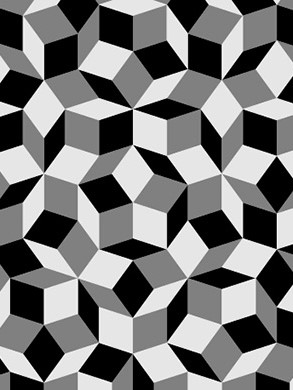
\includegraphics[width=0.6\linewidth]{images/penrose-bnw.jpg}

\vspace{2cm}

{\Huge Ryan Joo Rui An}
\nbvspace[1]
\end{center}

\thispagestyle{empty}
\pagebreak

\

\thispagestyle{empty}
\pagebreak

\begin{center}
\

\vspace{6cm}

{\huge\bfseries Undergraduate Mathematics}

\vspace{2cm}

{\huge Ryan Joo Rui An}
\end{center}
\thispagestyle{empty}
\pagebreak

\thispagestyle{empty}
\

\vfill

\begin{quote}
\textit{The mathematician does not study mathematics because it is useful; he studies it because he delights in it and he delights in it because it is beautiful.}

\begin{flushright}--- Henri Poincar\'{e} (1854--1912)\\
French mathematician and theoretical physicist\end{flushright}
\end{quote}

\vfill

Copyright \copyright \ 2024 by Ryan Joo Rui An.

Licensed under \href{https://creativecommons.org/licenses/by-nc-sa/4.0/}{CC BY-NC-SA 4.0}. You are free to copy and redistribute the material in any medium or format, as well as remix, transform, and build upon the material. You must give appropriate credit, provide a link to the license, and indicate if changes were made. You may do so in any reasonable manner, but not in any way that suggests the licensor endorses you or your use. You may not use the material for commercial purposes. If you remix, transform, or build upon the material, you must distribute your contributions under the same license as the original. You may not apply legal terms or technological measures that legally restrict others from doing anything the license permits.

This is (still!) an incomplete draft. Please send corrections and comments to \url{ryanjooruian18@gmail.com}, or pull-request at \url{https://github.com/Ryanjoo18/undergrad-math}.

Typeset using \LaTeX.

Last updated \today.
\pagebreak

\frontmatter
\section*{About the Author}
\textbf{Ryan Joo Rui An} is a high school student currently engaged in his A Level studies in Singapore. He has spent over 11 years honing his skills in various mathematics competitions. His journey began at an early age, where he developed a fascination with numbers while doing mental arithmetic. This early interest quickly blossomed into a deep commitment to mathematics, leading him to participate in numerous mathematics olympiads competitions.

The author's (not many) mathematics credentials include:
\begin{itemize}
\item 3 Silver awards in the \emph{Singapore Mathematics Olympiad} 2022 to 2024;
\item 6 Gold awards in the \emph{Singapore and Asian Schools Math Olympiad} 2019 to 2023, top in Singapore in 2022 and 2023, top in Malaysia in 2024;
\item Merit award in the \emph{Singapore International Mathematical and Computational Challenge} 2024;
\item 2 Prize awards, 2 High Distinction awards in the \emph{Australian Mathematics Competition} 2019 to 2023, best in school in 2023;
\item Honourable mention in the \emph{High School Mathematical Contest in Modeling} 2023;
\item 2nd place in the \emph{Hua Lo Geng Secondary School Mathematics Competition} 2019;
\item 1st place in the \emph{Chen Jingrun's Cup Secondary School Mathematics Competition} 2019.
\end{itemize}

Outside of mathematics, the author has a keen interest in playing chess and programming.

This book is a culmination of the author's years of experience, dedication, and love for mathematics while he studies mathematics at the undergraduate level.
\pagebreak

\section*{Preface}
\ifprelim
\cref{part:prelim} covers \textbf{preliminary topics}, which are crucial stepping stones for subsequent topics. This includes logic and methods of proofs in \cref{chap:logic-proofs}, and basic set theory in \cref{chap:set-theory}.
\else
\fi

\iflinalg
\cref{part:linear-algebra} covers \textbf{linear algebra}, which follows \cite{axler}. \cref{chap:vector-spaces} gives an introduction to vector spaces and subspaces. \cref{chap:finite-dim-vector-spaces} gives an overview of span, linear independence, bases and dimension. \cref{chap:linear-maps} goes through linear maps, kernel and image, matrices, invertibility and isomorphism, as well as products and quotients of vector spaces.
\else
\fi

\ifabsalg
\cref{part:abstract-algebra} covers \textbf{abstract algebra}, which follows \cite{dummit-foote,artin}. \cref{chap:group-theory} covers group theory.
\else
\fi

\ifranalysis
\cref{part:real-analysis} covers \textbf{real analysis}, which follows \cite{rudin,apostol,bartle-sherbert}. \cite{alcock} is also a good read to get some intuition into some abstract notions.
\else
\fi

\ifcanalysis
\cref{part:complex-analysis} covers \textbf{complex analysis}, which follows \cite{ahlfors,lang}.
\else
\fi

\iftop
\cref{part:topology} covers \textbf{topology}, which follows \cite{munkres}.
\else
\fi

%\item \textbf{calculus} which follows \cite{spivak,stewart}.

The chapters in this book are structured in the following typical manner. Each chapter begins with a \textbf{theoretical portion}, which starts off with a couple of definitions, followed by theorems, lemmas and propositions built upon the definitions. Each chapter is ended by some \textbf{exercises} accompanied by solutions to them.

The reader is not assumed to have any mathematical prerequisites, although some experience with proofs may be helpful.

\subsection*{Problem Solving}
Mathematics is about problem solving. In \cite{polya}, George P\'{o}lya outlined the following problem solving cycle.
\begin{enumerate}
\item \textbf{Understand the problem}

Ask yourself the following questions:
\begin{itemize}
\item Do you understand all the words used in stating the problem?
\item Is it possible to satisfy the condition? Is the condition sufficient to determine the unknown? Or is it insufficient? Or redundant? Or contradictory?
\item What are you asked to find or show? Can you restate the problem in your own words?
\item Draw a figure. Introduce suitable notation.
\item Is there enough information to enable you to find a solution?
\end{itemize}

\item \textbf{Devise a plan}

A partial list of heuristics -- good rules of thumb to solve problems -- is included:
\begin{multicols}{2}
\begin{itemize}
\item Guess and check
\item Look for a pattern
\item Make an orderly list
\item Draw a picture
\item Eliminate possibilities
\item Solve a simpler problem
\item Use symmetry
\item Use a model
\item Consider special cases
\item Work backwards
\item Use direct reasoning
\item Use a formula
\item Solve an equation
\item Be ingenious
\end{itemize}
\end{multicols}

\item \textbf{Execute the plan}

This step is usually easier than devising the plan. In general, all you need is care and patience, given that you have the necessary skills. Persist with the plan that you have chosen. If it continues not to work discard it and choose another. Don't be misled, this is how mathematics is done, even by professionals.

\begin{itemize}
\item Carrying out your plan of the solution, check each step. Can you see clearly that the step is correct? Can you prove that it is correct?
\end{itemize}

\item \textbf{Check and expand}

P\'{o}lya mentions that much can be gained by taking the time to reflect and look back at what you have done, what worked, and what didn't. Doing this will enable you to predict what strategy to use to solve future problems.

Look back reviewing and checking your results. Ask yourself the following questions:
\begin{itemize}
\item Can you check the result? Can you check the argument?
\item Can you derive the solution differently? Can you see it at a glance?
\item Can you use the result, or the method, for some other problem?
\end{itemize}
\end{enumerate}

Building on P\'{o}lya's problem solving strategy, Schoenfeld \cite{schoenfeld} came up with the following framework for problem solving, consisting of four components:
\begin{enumerate}
\item \textbf{Cognitive resources}: the body of facts and procedures at one's disposal.
\item \textbf{Heuristics}: `rules of thumb' for making progress in difficult situations.
\item \textbf{Control}: having to do with the efficiency with which individuals utilise the knowledge at their disposal. Sometimes, this is referred to as metacognition, which can be roughly translated as `thinking about one's own thinking'.
\begin{enumerate}
\item These are questions to ask oneself to monitor one's thinking.
\begin{itemize}
    \item What (exactly) am I doing? [Describe it precisely.] Be clear what I am doing NOW. Why am I doing it? [Tell how it fits into the solution.]
    \item Be clear what I am doing in the context of the BIG picture -- the solution. Be clear what I am going to do NEXT.
\end{itemize}

\item Stop and reassess your options when you
\begin{itemize}
    \item cannot answer the questions satisfactorily [probably you are on the wrong track]; OR
    \item are stuck in what you are doing [the track may not be right or it is right but it is at that moment too difficult for you].
\end{itemize}

\item Decide if you want to
\begin{itemize}
    \item carry on with the plan,
    \item abandon the plan, OR
    \item put on hold and try another plan.
\end{itemize}
\end{enumerate}

\item \textbf{Belief system}: one's perspectives regarding the nature of a discipline and how one goes about working on it.
\end{enumerate}

\subsection*{Reading Skills}
A mathematics book is not a storybook; it is imperative that you know how to read a mathematics book properly.
\begin{enumerate}[leftmargin=1.3cm]
\item[\textbf{Read 0}] Don't read the book, read the Wikipedia article about the subject. Learn about the big questions asked in the subject, and the basics of the theorems that answer them. Often the most important ideas are those that can be stated concisely, so you should be able to remember them once you are engaging the book.
\item[\textbf{Read 1}] Let your eyes jump from definition to lemma to theorem without reading the proofs in between unless something grabs your attention or bothers you. If the book has exercises, see if you can do the first one of each chapter or section as you go.
\item[\textbf{Read 2}] Read the book but this time read the proofs. But don't worry if you don't get all the details. If some logical jump doesn't make complete sense, feel free to ignore it at your discretion as long as you understand the overall flow of reasoning.
\item[\textbf{Read 3}] Read through the lens of a sceptic. Work through all of the proofs with a fine toothed comb, and ask yourself every question you think of. You should never have to ask yourself ``why'' you are proving what you are proving at this point, but you have a chance to get the details down.
\end{enumerate}

\subsection*{Study Skills}
The Faculty of Mathematics of the University of Cambridge has produced a leaflet called ``\href{https://www.maths.cam.ac.uk/undergrad/files/studyskills.pdf}{Study Skills in Mathematics}''. The Faculty also has \href{https://www.maths.cam.ac.uk/undergrad/files/Advice%20on%20Preparing%20for%20Exams%202022.pdf}{guidance notes} intended to help students prepare for exams.

Similarly, the Mathematical Institute of the University of Oxford has a \href{https://www.maths.ox.ac.uk/system/files/attachments/study_public_0.pdf}{study guide} and \href{https://www.maths.ox.ac.uk/system/files/attachments/Revision_advice_final_0.pdf}{thoughts on preparing for exams}.
\pagebreak

\tableofcontents
\pagebreak
%\printglossary[type=\acronymtype]

\mainmatter
%%%%%%%%%%%%%%% PRELIMINARY
\ifprelim
    \part{Preliminaries}\label{part:prelim}
    \chapter{Mathematical Reasoning and Logic}\label{chap:logic-proofs}
\section{Mathematical Terminology}
It is useful to be familiar with the following terminology.
\begin{itemize}
\item A \vocab{definition} is a precise and unambiguous description of the meaning of a mathematical term. It characterises the meaning of a word by giving all the properties and only those properties that must be true.
\item A \vocab{theorem} is a true mathematical statement that can be proven mathematically. In a mathematical paper, the term theorem is often reserved for the most important results.
\item A \vocab{lemma} is a minor result whose sole purpose is to help in proving a theorem. It is a stepping stone on the path to proving a theorem. Very occasionally lemmas can take on a life of their own.
\item A \vocab{corollary} is a result in which the (usually short) proof relies heavily on a given theorem.
\item A \vocab{proposition} is a proven and often interesting result, but generally less important than a theorem.
\item A \vocab{conjecture} is a statement that is unproved, but is believed to be true.
\item An \vocab{axiom} is a statement that is assumed to be true without proof. These are the basic building blocks from which all theorems are proven.
\item An \vocab{identity} is a mathematical expression giving the equality of two (often variable) quantities.
\item A \vocab{paradox} is a statement that can be shown, using a given set of axioms and definitions, to be both true and false. Paradoxes are often used to show the inconsistencies in a flawed theory.
\end{itemize}

A \vocab{proof} is a sequence of true statements, without logical gaps, that is a logical argument establishing some conclusion.

\section{Zeroth-order Logic}
A \vocab{proposition} is a sentence which has exactly one truth value, i.e. it is either true or false, but not both and not neither. A proposition is denoted by uppercase letters such as $P$ and $Q$. If the proposition $P$ depends on a variable $x$, it is sometimes helpful to denote it by $P(x)$. 

We can do some algebra on propositions, which include
\begin{enumerate}[label=(\roman*)]
\item \vocab{equivalence}, denoted by $P\iff Q$, which means $P$ and $Q$ are logically equivalent statements;

\item \vocab{conjunction}, denoted by $P\land Q$, which means ``$P$ and $Q$'';

\item \vocab{disjunction}, denoted by $P\lor Q$, which means ``$P$ or $Q$'';

\item \vocab{negation}, denoted by $\lnot P$, which means ``not $P$''.
\end{enumerate}

Here are some useful properties when handling logical statements. You can easily prove all of them using truth tables.
\begin{proposition}[Double negation law]
\[P\iff\lnot(\lnot P)\]
\end{proposition}

\begin{proposition}[Commutative property]
\[ P \land Q \iff Q \land P, \quad P \lor Q \iff Q \lor P \]
\end{proposition}

\begin{proposition}[Associative property for conjunction]
\[ (P\land Q)\land R \iff P\land (Q\land R) \]
\end{proposition}

\begin{proposition}[Associative property for disjunction]
\[ (P\lor Q)\lor R \iff P\lor (Q\lor R) \]
\end{proposition}

\begin{proposition}[Distributive property for conjunction across disjunction]
\[ P\land(Q\lor R) \iff (P\land Q)\lor(P\land Q) \]
\end{proposition}

\begin{proposition}[Distributive property for disjunction across conjunction]
\[ P\lor(Q\land R) \iff (P\lor Q)\land(P\lor R) \]
\end{proposition}

\begin{proposition}[De Morgan's laws]
\[ \lnot(P \lor Q) \iff (\lnot P \land \lnot Q) \]
\[ \lnot (P\land Q) \iff (\lnot P\lor \lnot Q) \]
\end{proposition}

\begin{exercise}
Negate the statement $1<x<2$.
\end{exercise}

\begin{solution}
\begin{align*}
\lnot(1<x<2)&\iff\lnot[(x>1)\land(x<2)]\\
&\iff\lnot(x>1)\lor\lnot(x<2)\\
&\iff(x\le1)\lor(x\ge2)
\end{align*}
where the last step follows from the trichotomy axiom of real numbers.
\end{solution}

\begin{exercise}
Negate the statement
\[n=2\quad\text{or}\quad n\text{ is odd.}\]
\end{exercise}

\begin{solution}
\begin{align*}
\lnot [(n = 2) \lor (n \text{ is odd})] &\iff \lnot(n = 2) \land \lnot(n \text{ is odd}) \\
&\iff (n \neq 2) \land (n \text{ is even})
\end{align*}
where we have used the fact that every integer is either even or odd, but not both.
\end{solution}
\pagebreak

\subsection{If, only if}
\vocab{Implication} is denoted by $P \implies Q$, which means ``$P$ implies $Q$'', i.e. if $P$ holds then $Q$ also holds. It is equivalent to saying ``If $P$ then $Q$''. The only case when $P \implies Q$ is false is when the hypothesis $P$ is true and the conclusion $Q$ is false.

$P \implies Q$ is known as a \vocab{conditional statement}. $P$ is known as the \vocab{hypothesis}, $Q$ is known as the \vocab{conclusion}.

Statements of this form are probably the most common, although they may sometimes appear quite differently. The following all mean the same thing:
\begin{enumerate}[label=(\roman*)]
\item if $P$ then $Q$;
\item $P$ implies $Q$;
\item $P$ only if $Q$;
\item $P$ is a sufficient condition for $Q$;
\item $Q$ is a necessary condition for $P$.
\end{enumerate}

The \vocab{converse} of $P \implies Q$ is given by $Q \implies P$; both are not logically equivalent.

The \vocab{inverse} of $P \implies Q$ is given by $\lnot P \implies \lnot Q$, i.e. the hypothesis and conclusion of the statement are both negated.

The \vocab{contrapositive} of $P \implies Q$ is given by $\lnot Q \implies \lnot P$; both are logically equivalent.

To prove $P \implies Q$, start by assuming that $P$ holds and try to deduce through some logical steps that $Q$ holds too. Alternatively, start by assuming that $Q$ does not hold and show that $P$ does not hold (that is, we prove the contrapositive).

\subsection{If and only if, iff}
\vocab{Bidirectional implication} is denoted by $P \iff Q$, which means both $P \implies Q$ and $Q \implies P$. We can read this as ``$P$ if and only if $Q$''. The letters ``iff'' are also commonly used to stand for ``if and only if''.

$P \iff Q$ is true exactly when $P$ and $Q$ have the same truth value.

$P \iff Q$ is known as a \vocab{biconditional statement}.

These statements are usually best thought of separately as ``if'' and ``only if'' statements.

To prove $P \iff Q$, prove the statement in both directions, i.e. prove both $P \implies Q$ and $Q \implies P$. Remember to make very clear, both to yourself and in your written proof, which direction you are doing.

\section{First-order Logic}
The \vocab{universal quantifier} is denoted by $\forall$, which means ``for all'' or ``for every''. An universal statement has the form $\forall x\in X, P(x)$.

The \vocab{existential quantifier} is denoted by $\exists$, which means ``there exists''. An existential statement has the form $\exists x\in X, P(x)$, where $X$ is known as the \vocab{domain}.

These are versions of De Morgan's laws for quantifiers:
\[ \lnot \forall x\in X,P(x) \iff \exists x\in X,\lnot P(x) \]
\[ \lnot \exists x\in X,P(x) \iff \forall x\in X,\lnot P(x) \]

\begin{exercise}
Negate the statement
\[ \text{for all real numbers } x, \text{ if } x>2, \text{ then } x^2>4 \]
\end{exercise}
\begin{solution}
In logical notation, this statement is $(\forall x \in \RR)[x>2 \implies x^2>4]$.
\begin{align*}
\lnot\{(\forall x \in \RR)[x>2 \implies x^2>4]\} 
&\iff (\exists x \in \RR) \lnot[x>2 \implies x^2>4] \\
&\iff (\exists x \in \RR) \lnot [(x\le2) \lor (x^2>4)] \\
&\iff (\exists x \in \RR) [(x>2) \land (x^2\le4)]
\end{align*}
\end{solution}

\begin{exercise}
Negate surjectivity.
\end{exercise}
\begin{solution}
If $f:X\to Y$ is not surjective, then it means that there exists $y \in Y$ not in the image of $X$, i.e. for all $x$ in $X$ we have $f(x)\neq y$.
\begin{align*}
\lnot \forall y \in Y, \exists x \in X, f(x)=y 
&\iff \exists y \in Y, \lnot (\exists x \in X, f(x)=y) \\
&\iff \exists y \in Y, \forall x \in X, \lnot (f(x)=y) \\
&\iff \exists y \in Y, \forall x \in X, f(x) \neq y
\end{align*}
\end{solution}

To prove a statement of the form $\forall x \in X \suchthat P(x)$, start the proof with ``Let $x \in X$.'' or ``Suppose $x \in X$ is given.'' to address the quantifier with an arbitrary $x$; provided no other assumptions about $x$ are made during the course of proving $P(x)$, this will prove the statement for all $x \in X$. 

To prove a statement of the form $\exists x \in X \suchthat P(x)$, there is not such a clear steer about how to continue: you may need to show the existence of an $x$ with the right properties; you may need to demonstrate logically that such an $x$ must exist because of some earlier assumption, or it may be that you can show constructively how to find one; or you may be able to prove by contradiction, supposing that there is no such $x$ and consequently arriving at some inconsistency.

\begin{remark}
Read from left to right, and as new elements or statements are introduced they are allowed to depend on previously introduced elements but cannot depend on things that are yet to be mentioned.
\end{remark}

\begin{remark}
To avoid confusion, it is a good idea to keep to the convention that the quantifiers come first, before any statement to which they relate.
\end{remark}
\pagebreak

\section{Proofs}
A \vocab{direct proof} of $P \implies Q$ is a series of valid arguments that start with the hypothesis $P$ and end with the conclusion $Q$. It may be that we can start from $P$ and work directly to $Q$, or it may be that we make use of $P$ along the way.

A \vocab{proof by contrapositive} of $P \implies Q$ is to prove instead $\lnot Q \implies \lnot P$.

A \vocab{disproof by counterexample} is to providing a counterexample in order to refute or disprove a conjecture. The counterexample must make the hypothesis a true statement, and the conclusion a false statement. In seeking counterexamples, it is a good idea to keep the cases you consider simple, rather than searching randomly. It is often helpful to consider ``extreme'' cases; for example, something is zero, a set is empty, or a function is constant.

A \vocab{proof by cases} is to first dividing the situation into cases which exhaust all the possibilities, and then show that the statement follows in all cases.

\subsection{Proof by contradiction}
A \vocab{proof by contradiction} of $P$ involves first supposing $P$ is false, i.e. $\lnot P$; to prove $P \implies Q$ by contradiction, suppose that $Q$ is false, i.e. $P\land\lnot Q$. Then show through some logical reasoning that this leads to a contradiction or inconsistency. We may arrive at something that contradicts the hypothesis $P$, or something that contradicts the initial supposition that $Q$ is not true, or we may arrive at something that we know to be universally false.

\begin{exercise}[Irrationality of $\sqrt{2}$]
Prove that $\sqrt{2}$ is irrational.
\end{exercise}
\begin{proof}
We prove by contradiction. Suppose otherwise, that $\sqrt{2}$ is rational. Then $\sqrt{2}=\dfrac{a}{b}$ for some $a,b\in\ZZ,b\neq 0$, $a,b$ coprime.

Squaring both sides gives
\[a^2=2b^2.\]
Since RHS is even, LHS must also be even. Hence it follows that $a$ is even. Let $a=2k$ where $k\in\ZZ$. Substituting $a = 2k$ into the above equation and simplifying it gives us
\[b^2=2k^2.\]
This means that $b^2$ is even, from which follows again that $b$ is even. 

This contradicts the assumption that $a,b$ coprime. Hence proven.
\end{proof}

\begin{exercise}[Euclid's theorem]
There are infinitely many prime numbers.
\end{exercise}

\begin{proof}
Suppose otherwise, that only finitely many prime numbers exist. List them as $p_1,\dots,p_n$. The number $N=p_1p_2\cdots p_n+1$ is divisible by a prime $p$, yet is coprime to $p_1,\dots,p_n$. Therefore, $p$ does not belong to our list of all prime numbers, a contradiction. Hence the initial assumption was false, proving that there are infinitely many primes.
\end{proof}

To \vocab{prove uniqueness}, we can either assume $\exists x,y \in S$ such that $P(x) \land P(y)$ is true and show $x=y$, or argue by assuming that $\exists x,y \in S$ are distinct such that $P(x) \land P(y)$, then derive a contradiction. $\exists!$ denotes ``there exists a unique''. To prove uniqueness and existence, we also need to show that $\exists x \in S \suchthat P(x)$ is true.

\subsection{Proof of existence}
To prove existential statements, we can adopt two approaches:
\begin{enumerate}
\item Constructive proof (direct proof): 

To prove statements of the form $\exists x\in X \suchthat P(x)$, find or construct \vocab{a specific example} for $x$. To prove statements of the form $\forall y\in Y,\:\exists x\in X\suchthat P(x,y)$, construct example for $x$ \vocab{in terms of $y$} (since $x$ is dependent on $y$).

In both cases, you have to justify that your example $x$
\begin{enumerate}
\item belongs to the domain $X$, and
\item satisfies the condition $P$.
\end{enumerate}

\item Non-constructive proof (indirect proof): 

Use when specific examples are not easy or not possible to find or construct.
Make arguments why such objects have to exist.
May need to use proof by contradiction.
Use definition, axioms or results that involve existential statements.
\end{enumerate}

\begin{exercise}
Prove that we can find $100$ consecutive positive integers which are all composite numbers.
\end{exercise}

\begin{proof}
We can prove this existential statement via constructive proof.

Our goal is to find integers $n,n+1,n+2,\dots,n+99$, all of which are composite.

Take $n=101!+2$. Then $n$ has a factor of $2$ and hence is composite. Similarly, $n+k=101!+(k+2)$ has a factor $k+2$ and hence is composite for $k=1,2,\dots,99$.

Hence the existential statement is proven.
\end{proof}

\begin{exercise}
Prove that for all rational numbers $p$ and $q$ with $p<q$, there is a rational number $x$ such that $p<x<q$.
\end{exercise}
\begin{proof}
We prove this by construction. Our goal is to find such a rational $x$ \vocab{in terms of $p$ and $q$}.

We take the average. Let $x=\dfrac{p+q}{2}$ which is a rational number.

Since $p<q$, 
\[ x=\frac{p+q}{2}<\frac{q+q}{2}=q \implies x<q \]
Similarly,
\[ x=\frac{p+q}{2}>\frac{p+p}{2}=p \implies p<x \]
Hence we have shown the existence of rational number $x$ such that $p<x<q$.

\begin{remark}
For this type of question, there are two parts to prove: firstly, $x$ satisfies the given statement; secondly, $x$ is within the domain (for this question we do not have to prove $x$ is rational since $\QQ$ is closed under addition).
\end{remark}
\end{proof}

\begin{exercise}
Prove that for all rational numbers $p$ and $q$ with $p<q$, there is an irrational number $r$ such that $p<r<q$.
\end{exercise}
\begin{proof}
We prove this by construction. Similarly, our goal is to find an irrational $r$ in terms of $p$ and $q$.

Note that we cannot simply take $r=\dfrac{p+q}{2}$; a simple counterexample is the case $p=-1,q=1$ where $r=0$ is clearly not irrational.

Since $p$ lies in between $p$ and $q$, let $r=p+c$ where $0<c<q-p$. Since $c<q-p$, we have $c=\dfrac{q-p}{k}$ for some $k>1$; to make $c$ irrational, we take $k$ to be irrational.

Take $r=p+\dfrac{q-p}{\sqrt{2}}$. We need to show $r$ is irrational and $p<r<q$.

\textbf{Part 1:} $p<r<q$

Since $q<p$, $r=p+\text{(positive number)}>p$. On the other hand, $\dfrac{q-p}{\sqrt{2}}<q-p$ so $r<p+(q-p)=q$.

\textbf{Part 2:} $r$ is irrational

We prove by contradiction. Suppose $r$ is rational. We have $\sqrt{2}=\dfrac{q-p}{r-p}$. Since $p,q,r$ are all rational (and $r-p\neq0$), RHS is rational. This implies that LHS is rational, i.e. $\sqrt{2}$ is rational, a contradiction.
\end{proof}

\subsubsection{Non-constructive proof}


\begin{exercise}{}{}
Prove that every integer greater than $1$ is divisible by a prime.
\end{exercise}

\begin{proof}
If $n$ is prime, then we are done as $n\mid n$.

If $n$ is not prime, then $n$ is composite. So $n$ has a divisor $d_1$ such that $1<d_1<n$. If $d_1$ is prime then we are done as $d_1\mid n$. If $d_1$ is not prime then $d_1$ is composite, has divisor $d_2$ such that $1<d_2<n$.

If $d_2$ is prime, then we are done as $d_2\mid d_1$ and $d_1\mid n$ imply $d_2\mid n$. If $d_2$ is not prime then $d_2$ is composite, has divisor $d_3$ such that $1<d_3<d_2$.

Continuing in this manner after $k$ times, we will get
\[ 1<d_k<d_{k-1}<\cdots<d_2<d_1<n \]
where $d_i\mid n$ for all $i$.

This process must stop after finite steps, as there can only be a finite number of $d_i$'s between $1$ and $n$. On the other hand, the process will stop only if there is a $d_i$ which is a prime. 

Hence we conclude that there must be a divisor $d_i$ of $n$ that is prime.
\end{proof}

\begin{remark}
This proof is also known as \vocab{proof by infinite descent}, a method which relies on the well-ordering principle of the positive integers.
\end{remark}

\begin{exercise}{}{}
Prove that the equation $x^2+y^2=3z^2$ has no solutions $(x,y,z)$ in integers where $z\neq0$.
\end{exercise}

\begin{proof}
Suppose we have a solution $(x,y,z)$. Without loss of generality, we may assume that $z>0$. By the least integer principle, we may also assume that our solution has $z$ minimal. Taking remainders modulo $3$, we see that
\[ x^2+y^2\equiv0\pmod3 \]
Recalling that squares may only be congruent to $0$ or $1$ modulo $3$, we conclude that
\[ x^2\equiv y^2\equiv 0 \implies x \equiv y \equiv 0 \pmod 3 \]
Writing $x=3a$ and $y=3b$ we obtain
\[ 9a^2+9b^2=3z^2 \implies 3(a^2+b^2)=z^2 \implies 3\mid z^2 \implies 3\mid z \]
Now let $z=3c$ and cancel $3$'s to obtain
\[ a^2+b^2=3c^2. \]
We have therefore constructed another solution $(a,b,c)=\brac{\frac{x}{3},\frac{y}{3},\frac{z}{3}}$ to the original equation. However $0<c<z$ contradicts the minimality of $z$.
\end{proof}

\subsection{Proof by mathematical induction}
Induction is an extremely powerful method of proof used throughout mathematics. It deals with infinite families of statements which come in the form of lists. The idea behind induction is in showing how each statement follows from the previous one on the list -- all that remains is to kick off this logical chain reaction from some starting point.

\begin{theorem}[Principle of Mathematical Induction]
Let $P(n)$ be a family of statements indexed by $\ZZ^+$. Suppose that 
\begin{enumerate}[label=(\roman*)]
\item (\textbf{base case}) $P(1)$ is true and
\item (\textbf{inductive step}) for all $k\in\ZZ^+$, $P(k)\implies P(k+1)$.
\end{enumerate}
Then $P(n)$ is true for all $n\in\ZZ^+$.
\end{theorem}

Using logic notation, this is written as
\[ \{P(1) \land (\forall n \in \ZZ^+) [P(k) \implies P(k+1)]\} \implies (\forall n \in \ZZ^+)P(n) \]

\begin{remark}
Induction is often visualised like toppling dominoes. The inductive step (ii) corresponds to placing each domino sufficiently close that it will be hit when the previous one falls over, and base case (i) corresponds to knocking over the first one.
\[ P(1) \implies P(2) \implies \cdots \implies P(k) \implies P(k+1) \implies \cdots \]
\end{remark}

To practise, we go through a classic proof using induction.

\begin{exercise}
Prove that for any $n\in\ZZ^+$,
\[\sum_{i=1}^n i=\frac{n(n+1)}{2}.\]
\end{exercise}

\begin{proof}
Let $\displaystyle P(n):\sum_{i=1}^n i=\frac{n(n+1)}{2}$.

Clearly $P(1)$ holds. Now suppose $P(k)$ holds for some $k\in\ZZ^+$, $k\ge1$; that is,
\[\sum_{i=1}^k i=\frac{k(k+1)}{2}.\]
Adding $k+1$ to both sides,
\begin{align*}
\sum_{i=1}^{k+1} i&=\frac{k(k+1)}{2}+(k+1)\\
&=\frac{(k+1)(k+2)}{2}\\
&=\frac{(k+1)[(k+1)+1]}{2}
\end{align*}
thus $P(k+1)$ is true.

Since $P(1)$ true and $P(k)\implies P(k+1)$ for all $k\in\ZZ^+$, $k\ge1$,\\
$P(n)$ is true for all $n\in\ZZ^+$.
\end{proof}

A corollary of induction is if the family of statements holds for $n \ge N$, rather than necessarily $n \ge 0$:

\begin{corollary}
Let $N$ be an integer and let $P(n)$ be a family of statements indexed by integers $n \ge N$. Suppose that 
\begin{enumerate}[label=(\roman*)]
\item (\textbf{base case}) $P(N)$ is true and
\item (\textbf{inductive step}) for all $k \ge N$, $P(k) \implies P(k+1)$. 
\end{enumerate}
Then $P(n)$ is true for all $n \ge N$.
\end{corollary}

\begin{proof}
This follows directly by applying the above theorem to the statement $Q(n) = P(n+N)$ for $n \in N$.
\end{proof}

\subsubsection{Strong induction}
Another variant on induction is when the inductive step relies on some earlier case(s) but not necessarily the immediately previous case. This is known as \vocab{strong induction}:

\begin{theorem}[Strong Form of Induction]
Let $P(n)$ be a family of statements indexed by the natural numbers. Suppose that
\begin{enumerate}[label=(\roman*)]
\item (\textbf{base case}) $P(1)$ is true and
\item (\textbf{inductive step}) for all $m \in \ZZ^+$, if for integers $k$ with $1 \le k \le m$, $P(k)$ is true then $P(m+1)$ is true.
\end{enumerate}
Then $P(n)$ is true for all $n \in \NN$.
\end{theorem}

Using logic notation, this is written as
\[ \{P(1) \land (\forall m \in \ZZ^+) [P(1) \land P(2) \land \cdots \land P(m) \implies P(m+1)]\} \implies (\forall n \in \ZZ^+)P(n) \]

\begin{proof}
We can this it to an instance of ``normal'' induction by defining a related family of statements $Q(n)$. 

Let $Q(n)$ be the statement ``$P(k)$ holds for $k=0,1,\dots,n$''. Then the conditions for the strong form are equivalent to 
\begin{enumerate}[label=(\roman*)]
\item $Q(0)$ holds and 
\item for any $n$, if $Q(n)$ is true then $Q(n+1)$ is also true.
\end{enumerate}
It follows by induction that $Q(n)$ holds for all $n$, and hence $P(n)$ holds for all $n$.
\end{proof}

The following example illustrates how the strong form of induction can be useful:

\begin{example}[Fundamental Theorem of Arithmetic]
Every natural number greater than 1 may be expressed as a product of one or more prime numbers.
\end{example}

\begin{proof}
Let $P(n)$ be the statement that $n$ may be expressed as a product of prime numbers. 

Clearly $P(2)$ holds, since $2$ is itself prime. 

Let $n \ge 2$ be a natural number and suppose that $P(m)$ holds for all $m<n$.

\begin{itemize}
\item If $n$ is prime then it is trivially the product of the single prime number $n$. 

\item If $n$ is not prime, then there must exist some $r, s > 1$ such that $n = rs$. By the inductive hypothesis, each of $r$ and $s$ can be written as a product of primes, and therefore $n = rs$ is also a product of primes.
\end{itemize}

Thus, whether $n$ is prime or not, we have have that $P(n)$ holds. By strong induction, $P(n)$ is true for all natural numbers. That is, every natural number greater than 1 may be expressed as a product of one or more primes.
\end{proof}

\subsubsection{Cauchy induction}
\begin{theorem}[Cauchy Induction]
Let $P(n)$ be a family of statements indexed by $\ZZ^+_{\ge2}$. Suppose that
\begin{enumerate}[label=(\roman*)]
\item (\textbf{base case}) $P(2)$ is true and
\item (\textbf{inductive step}) for all $k\in\ZZ^+$, $P(k)\implies P(2k)$ and $P(k)\implies (k-1)$.
\end{enumerate}
Then $P(n)$ is true for all $n\in\ZZ^+_{\ge2}$.
\end{theorem}

\begin{exercise}{}{}
Using Cauchy Induction, prove the AM--GM Inequality for $n$ variables, which states that for positive reals $a_1, a_2,\dots a_n$,
\[ \frac{a_1+a_2+\cdots+a_n}{n}\ge\sqrt[n]{a_1a_2\cdots a_n}. \]
\end{exercise}
\begin{proof}
Let $P(n)$ be $\frac{a_1+a_2+\cdots+a_n}{n}\ge\sqrt[n]{a_1a_2\cdots a_n}$.

Base case $P(2)$ is true because\[\frac{a_1+a_2}{2}\ge\sqrt{a_1a_2} \iff (a_1+a_2)^2\ge 4a_1a_2 \iff (a_1-a_2)^2\ge0\]

Next we show that $P(n)\implies P(2n)$, i.e. if AM--GM holds for $n$ variables, it also holds for $2n$ variables:

\[\frac{a_1+a_2+\cdots+a_{2n}}{2n}=\frac{\frac{a_1+a_2+\cdots+a_n}{n}+\frac{a_{n+1}+a_{n+2}+\cdots+a_{2n}}{n}}{2}\]\[\frac{\frac{a_1+a_2+\cdots+a_n}{n}+\frac{a_{n+1}+a_{n+2}+\cdots+a_{2n}}{n}}{2}\ge\frac{\sqrt[n]{a_1a_2\cdots a_n}+\sqrt[n]{a_{n+1}a_{n+2}\cdots a_{2n}}}{2}\]\[\frac{\sqrt[n]{a_1a_2\cdots a_n}+\sqrt[n]{a_{n+1}a_{n+2}\cdots a_{2n}}}{2}\ge\sqrt{\sqrt[n]{a_1a_2\cdots a_n}\sqrt[n]{a_{n+1}a_{n+2}\cdots a_{2n}}}\]\[\sqrt{\sqrt[n]{a_1a_2\cdots a_n}\sqrt[n]{a_{n+1}a_{n+2}\cdots a_{2n}}}=\sqrt[2n]{a_1a_2\cdots a_{2n}}\]
The first inequality follows from $n$-variable AM--GM, which is true by assumption, and the second inequality follows from 2-variable AM--GM, which is proven above.

Finally we show that $P(n)\implies P(n-1)$, i.e. if AM--GM holds for $n$ variables, it also holds for $n-1$ variables. By $n$-variable AM--GM, $\frac{a_1+a_2+\cdots+a_n}{n}\ge\sqrt[n]{a_1a_2\cdots a_n}$ Let $a_n=\frac{a_1+a_2+\cdots+a_{n-1}}{n-1}$ Then we have\[\frac{a_1+a_2+\cdots+a_{n-1}+\frac{a_1+a_2+\cdots+a_{n-1}}{n-1}}{n}=\frac{a_1+a_2+\cdots+a_{n-1}}{n-1}\]So,\[\frac{a_1+a_2+\cdots+a_{n-1}}{n-1}\ge\sqrt[n]{a_1a_2\cdots a_{n-1}\cdot \frac{a_1+a_2+\cdots+a_{n-1}}{n-1}}\]\[\Rightarrow\left(\frac{a_1+a_2+\cdots+a_{n-1}}{n-1}\right)^n\ge a_1a_2\cdots a_{n-1}\cdot \frac{a_1+a_2+\cdots+a_{n-1}}{n-1}\]\[\Rightarrow\left(\frac{a_1+a_2+\cdots+a_{n-1}}{n-1}\right)^{n-1}\ge a_1a_2\cdots a_{n-1}\]\[\Rightarrow \frac{a_1+a_2+\cdots+a_{n-1}}{n-1}\ge\sqrt[n-1]{a_1a_2\cdots a_{n-1}}\]
By Cauchy Induction, this proves the AM--GM inequality for $n$ variables.
\end{proof}

\subsubsection{Other variations}
Apart from proving $P(n)$ indexed by $\ZZ^+$, we can also use PMI to prove statements of the form
\begin{itemize}
\item $(\forall n\in\ZZ) P(n)$

\textbf{Base case:} $P(0)$

\textbf{Inductive step:} $(\forall k\in\ZZ_{\ge0}) P(k)\implies P(k+1)$ and $(\forall k\in\ZZ_{\le0}) P(k)\implies P(k-1)$
\[ \cdots \Longleftarrow P(-n) \Longleftarrow \cdots \Longleftarrow P(-1) \Longleftarrow P(0) \implies P(1) \implies \cdots \implies P(n) \implies \cdots \]

\item $(\forall n\in\QQ) P(n)$

\textbf{Base case:} $P(0)$

\textbf{Inductive step:} $P(x)\implies P(-x)$ and $P\brac{\frac{a}{b}}\implies P\brac{\frac{a+1}{b}}$ and $P\brac{\frac{a}{b}}\implies P\brac{\frac{a}{b+1}}$
\end{itemize}

\subsubsection{A more generalised version}
\begin{definition}
A binary relation $\preceq$ on $X$ that satisfies the following conditions is called a \vocab{well-ordering} on $X$:
\begin{enumerate}[label=(\roman*)]
\item for every $a,b\in X$, $a\preceq b$ or $b\preceq a$,
\item every non-empty subset $S$ of $X$ contains a least element wrt $\preceq$.
\end{enumerate}
\end{definition}

\begin{theorem}[Well-ordering principle]
Let $(X,\preceq)$ be a well-ordered set, with the least element $x_0$. Then $P(x)$ holds for all $x\in X$ if the following conditions hold:
\begin{enumerate}[label=(\roman*)]
\item (\textbf{base case}) $P(x_0)$ holds
\item (\textbf{inductive step}) $\forall x^\prime\prec x$, $P(x^\prime)\implies P(x)$
\end{enumerate}
\end{theorem}

\subsection{Pigeonhole principle}
\begin{theorem}[Pigeonhole principle]
If $kn+1$ objects ($k\ge1$ not necessarily finite) are distributed among $n$ boxes, one of the boxes will contain at least $k+1$ objects.
\end{theorem}

\begin{exercise}[IMO 1972]
Prove that every set of 10 two-digit integer numbers has two disjoint subsets with the same sum of elements.
\end{exercise}

\begin{solution}
Let $S$ be the set of $10$ numbers. It has $2^{10}-2=1022$ subsets that differ from both $S$ and the empty set. They are the ``pigeons''.

If $A\subset S$, the sum of elements of $A$ cannot exceed $91+92+\cdots+99=855$. The numbers between 1 and 855, which are all possible sums, are the ``holes''.

Because the number of ``pigeons'' exceeds the number of ``holes'', there will be two ``pigeons'' in the same ``hole''. Specifically, there will be two subsets with the same sum of elements. Deleting the common elements, we obtain two disjoint sets with the same sum of elements.
\end{solution}

\begin{exercise}[Putnam 2006]
Prove that for every set $X=\{x_1,x_2,\dots,x_n\}$ of $n$ real numbers, there exists a nonempty subset $S$ of $X$ and an integer $m$ such that
\[\absolute{m+\sum_{x\in S}s}\le\frac{1}{n+1}.\]
\end{exercise}

\begin{solution}
Recall that the fractional part of a real number $x$ is $x-\floor{x}$. Let us look at the fractional parts of the numbers $x_1,x_1+x_2,\dots,x_1+x_2+\cdots+x_n$. If any of them is either in the interval $\sqbrac{0,\frac{1}{n+1}}$ or $\sqbrac{\frac{n}{n+1},1}$, then we are done. If not, we consider these $n$ numbers as the ``pigeons'' and the $n-1$ intervals $\sqbrac{\frac{1}{n+1},\frac{2}{n+1}},\sqbrac{\frac{2}{n+1},\frac{3}{n+1}},\dots,\sqbrac{\frac{n-1}{n+1},\frac{n}{n+1}}$ as the ``holes''. By the pigeonhole principle, two of these sums, say $x_1+x_2+\cdots+x_k$ and $x_1+x_2+\cdots+x_{k+m}$, belong to the same interval. But then their difference $x_{k+1}+\cdots+x_{k+m}$ lies within a distance of $\frac{1}{n+1}$ of an integer, and we are done.
\end{solution}
\pagebreak

\section*{Exercises}
\begin{prbm}
Use the Unique Factorisation Theorem to prove that, if a positive integer $n$ is not a perfect square, then $\sqrt{n}$ is irrational.

[The Unique Factorisation Theorem states that every integer $n>1$ has a unique standard factored form, i.e. there is exactly one way to express $n=p_1^{k_1}p_2^{k_2}\cdots p_t^{k_t}$ where $p_1<p_2<\cdots<p_t$ are distinct primes and $k_1,k_2,\dots,k_t$ are some positive integers.]
\end{prbm}

\begin{proof}
Prove by contradiction.

Suppose $n$ is not a perfect square and $\sqrt{n}$ is rational.

Then $\sqrt{n}=\frac{a}{b}$ for some integers $a$ and $b$. Squaring both sides and clearing denominator gives 
\begin{equation*}\tag{$\ast$}
nb^2=a^2.
\end{equation*}

Consider the standard factored forms of $n$, $a$ and $b$:
\[ n=p_1^{k_1}p_2^{k_2}\cdots p_t^{k_t} \]
\[ a=q_1^{e_1}q_2^{e_2}\cdots q_u^{e_u} \implies a^2=q_1^{2e_1}q_2^{2e_2}\cdots q_u^{2e_u} \]
\[ b=r_1^{f_1}r_2^{f_2}\cdots r_v^{f_v} \implies b^2=r_1^{2f_1}r_2^{2f_2}\cdots r_v^{2f_v} \]
i.e. the powers of primes in the standard factored form of $a^2$ and $b^2$ are all even integers. 

This means the powers $k_i$ of primes $p_i$ in the standard factored form of $n$ are also even by Unique Factorisation Theorem (UFT):

Note that all $p_i$ appear in the standard factored form of $a^2$ with even power $2c_i$, because of $(\ast)$. By UFT, $p_i$ must also appear in the standard factored form of $nb^2$ with the same even power $2c_i$.

If $p_i\nmid b$, then $k_i=2c_i$ which is even. If $p_i\mid b$, then $p_i$ will appear in $b^2$ with even power $2d_i$. So $k_i+2d_i=2c_i$, and hence $k_i=2(c_i-d_i)$, which is again even.

Hence $n=p_1^{k_1}p_2^{k_2}\cdots p_t^{k_t}=\brac{p_1^{\frac{k_1}{2}}p_2^{\frac{k_2}{2}}\cdots p_t^{\frac{k_t}{2}}}^2$.

Since $\frac{k_i}{2}$ are all integers, $p_1^{\frac{k_1}{2}}p_2^{\frac{k_2}{2}}\cdots p_t^{\frac{k_t}{2}}$ is an integer and $n$ is a perfect square. This contradicts the given hypothesis that $n$ is not a perfect square.

So we conclude that when a positive integer $n$ is not a perfect square, then $\sqrt{n}$ is irrational.
\end{proof}

\begin{prbm}
Prove that for every pair of irrational numbers $p$ and $q$ such that $p<q$, there is an irrational $x$ such that $p<x<q$.
\end{prbm}

\begin{proof}
Consider the average of $p$ and $q$: $p<\dfrac{p+q}{2}<q$.

If $\dfrac{p+q}{2}$ is irrational, take $x=\dfrac{p+q}{2}$ and we are done.

If $\dfrac{p+q}{2}$ is rational, call it $r$, take the average of $p$ and $r$: $p<\dfrac{p+r}{2}<r<q$. Since $p$ is irrational and $r$ is rational, $\dfrac{p+r}{2}$ is irrational. In this case, we take $x=\dfrac{3p+q}{4}$.
\end{proof}

\begin{prbm}
Given $n$ real numbers $a_1,a_2,\dots,a_n$. Show that there exists an $a_i$ ($1\le i\le n$) such that $a_i$ is greater than or equal to the mean (average) value of the $n$ numbers.
\end{prbm}

\begin{proof}
Prove by contradiction.

Let $\bar{a}$ denote the mean value of the $n$ given numbers. Suppose $a_i<\bar{a}$ for all $a_i$. Then
\[ \bar{a}=\frac{a_1+a_2+\cdots+a_n}{n}<\frac{\bar{a}+\bar{a}+\cdots+\bar{a}}{n}=\frac{n\bar{a}}{n}=\bar{a}. \]
We derive $\bar{a}<\bar{a}$, which is a contradiction.

Hence there must be some $a_i$ such that $a_i>\bar{a}$.
\end{proof}

\begin{prbm}
Prove that the following statement is false: there is an irrational number $a$ such that for all irrational number $b$, $ab$ is rational.
\end{prbm}

\textbf{Thought process:} prove the negation of the statement: for every irrational number $a$, there is an irrational number $b$ such that $ab$ is irrational.

\textbf{Proving technique:} constructive proof (note that we can consider multiple cases and construct more than one $b$)

\begin{proof}
Given an irrational number $a$, let us consider $\dfrac{\sqrt{2}}{a}$.

\textbf{Case 1:} $\dfrac{\sqrt{2}}{a}$ is irrational.

Take $b=\dfrac{\sqrt{2}}{a}$. Then $ab=\sqrt{2}$ which is irrational.

\textbf{Case 2:} $\dfrac{\sqrt{2}}{a}$ is rational.

Then the reciprocal $\dfrac{a}{\sqrt{2}}$. Since $\sqrt{6}$ is irrational, the product $\brac{\dfrac{a}{\sqrt{2}}}\sqrt{6}=a\sqrt{3}$ is irrational. Take $b=\sqrt{3}$, which is irrational. Then $ab=a\sqrt{3}$ which is irrational.
\end{proof}

\begin{prbm}
Prove that there are infinitely many prime numbers that are congruent to $3$ modulo $4$.
\end{prbm}

\begin{proof}
Prove by contradiction.

Suppose there are only finitely many primes that are congruent to $3$ modulo $4$. Let $p_1,p_2,\dots,p_m$ be the list of all the primes that are congruent to $3$ modulo $4$.

We construct an integer $M$ by $M=(p_1p_2\cdots p_m)^2+2$.

We have the following observation:
\begin{enumerate}[label=(\roman*)]
\item  $M\equiv 3 \mod 4$.
\item Every $p_i$ divides $M-2$.
\item None of the $p_i$ divides $M$. [Otherwise, together with (ii), this will imply $p_i$ divides $2$, which is impossible.]
\item $M$ is not a prime number. [Otherwise, by (i), $M$ is a prime number congruent to $3$ modulo $4$. But $M\neq p_i$ for all $1\le i\le m$. This contradicts the assumption that $p_1,p_2,\dots,p_m$ are all the prime numbers congruent to $3$ modulo $4$.]
\end{enumerate}

From the above discussion, we know that $M$ is a composite number by (iv). So it has a prime factorization $M=q_1q_2\cdots q_k$.

Since $M$ is odd, all these prime factors $q_j$ must be odd, and hence $q_j$ must be congruent to either $1$ or $3$ modulo $4$.

By (iii), $q_j$ cannot be any of the $p_i$. So all $q_j$ must be congruent to $1$ modulo $4$. Then $M$, which is the product of $q_j$, must also be congruent to $1$ modulo $4$.

This contradicts (i) that $M$ is congruent to $3$ modulo $4$.

Hence we conclude that there must be infinitely many primes that are congruent to $3$ modulo $4$.
\end{proof}

\begin{prbm}
Prove that, for any positive integer $n$, there is a perfect square $m^2$ ($m$ is an integer) such that $n\le m^2\le 2n$.
\end{prbm}

\begin{proof}
Prove by contradiction.

Suppose otherwise, that $n>m^2$ and $(m+1)^2>2n$ so that there is no square between $n$ and $2n$, then
\[ (m+1)^2>2n>2m^2. \]
Since we are dealing with integers and the inequalities are strict, we get
\[ (m+1)^2\ge2m^2+2 \]
which simplifies to
\[ 0\ge m^2-2m+1=(m-1)^2 \]
The only value for which this is possible is $m=1$, but you can eliminate that easily enough.
\end{proof}

\begin{prbm}
Prove that for every positive integer $n\ge4$,
\[ n!>2^n. \]
\end{prbm}

\begin{proof}
Let $P(n):n!>2^n$

\textbf{Base case:} $P(4)$

LHS: $4!=4\times3\times2\times1=24$, RHS: $2^4=16<24$

So $P(4)$ is true.

\textbf{Inductive step:} $P(k) \implies P(k+1)$ for all $k\in\ZZ^+_{\ge4}$
\begin{align*}
k! &> 2^k \\
(k+1)k! &> 2^k(k+1) \\
&> 2^k2 \quad \text{since from $k\ge4$, $k+1\ge5>2$} \\
&= 2^{k+1}
\end{align*}
hence proven $P(k) \implies P(k+1)$ for integers $k\ge4$.

By PMI, we have proven $P(n)$ for all integers $n\ge4$.
\end{proof}

\begin{prbm}
Prove by mathematical induction, for $n\ge2$,
\[ \sqrt[n]{n}<2-\frac{1}{n}. \]
\end{prbm}

\begin{proof}
Let $P(n):\sqrt[n]{n}<2 - \dfrac{1}{n}$ for $n \ge 2$.

\textbf{Base case:} $P(2)$

When $n=2$, $\sqrt{2}=1.41\dots<2-\dfrac{1}{2}=1.5$ which is true. Hence $P(2)$ is true.

\textbf{Inductive step:} $P(k)\implies P(k+1)$ for all $k\in\ZZ^+_{\ge2}$

Assume $P(k)$ is true for $k \ge 2, k \in \ZZ^+$, i.e.
\[ \sqrt[k]{k}<2 - \dfrac{1}{k} \implies k<\brac{2-\frac{1}{k}}^k \]

We want to prove that $P(k+1)$ is true, i.e.
\[ k+1<\brac{2-\frac{1}{k+1}}^{k+1} \]

Since $k>2$, we have 
\begin{align*}
\brac{2-\frac{1}{k+1}}^{k+1}
&> \brac{2-\frac{1}{k}}^{k+1} \quad \because k>2 \\
&= \brac{2-\frac{1}{k}}^k\brac{2-\frac{1}{k}} \\
&> k\brac{2-\frac{1}{k}} \quad \text{[by inductive hypothesis]} \\
&= 2k-1=k+k-1 > k-1 \because k>2
\end{align*}
Hence $P(k+1)$ is true.

Since $P(2)$ is true and $P(k)\implies P(k+1)$, by mathematical induction $P(n)$ is true.
\end{proof}

\begin{prbm}
Prove that for all integers $n \ge 3$, 
\[ \brac{1+\frac{1}{n}}^n<n \]
\end{prbm}

\begin{proof}
\textbf{Base case:} $P(3)$

On the LHS, $\brac{1+\dfrac{1}{3}}^3=\dfrac{64}{27}=2\dfrac{10}{27}<3$. Hence $P(3)$ is true.

\textbf{Inductive step:} $P(k)\implies P(k+1)$ for all $k\in\ZZ^+_{\ge3}$

Our inductive hypothesis is
\[ \brac{1+\frac{1}{k}}^k<k \]
Multiplying both sides by $\brac{1+\dfrac{1}{k}}$ (to get a $k+1$ in the power),
\[ \brac{1+\frac{1}{k}}^k\brac{1+\frac{1}{k}}=\brac{1+\frac{1}{k}}^{k+1}<k\brac{1+\frac{1}{k}}=k+1  \]
Since $k<k+1 \iff \dfrac{1}{k}>\dfrac{1}{k+1}$, 
\[ \brac{1+\frac{1}{k}}^{k+1} > \brac{1+\frac{1}{k+1}}^{k+1} \]
The rest of the proof follows easily.
\end{proof}

A sequence of integers $F_i$, where integer $1\le i\le n$, is called the \vocab{Fibonacci sequence} if and only if it is defined recursively by $F_1=1$, $F_2=1$, $F_n=F_{n-1}+F_{n-2}$ for $n>2$.

\begin{prbm}
Let $a_i$ where integer $1\le i\le n$ be a sequence of integers defined recursively by initial conditions $a_1=1$, $a_2=1$, $a_3=3$ and the recurrence relation $a_n=a_{n-1}+a_{n-2}+a_{n-3}$ for $n>3$.

For all $n\in\ZZ^+$, prove that
\[ a_n\le2^{n-1}. \]
\end{prbm}

\begin{proof}
Let $P(n):a_n\le2^{n-1}$.

Given the recurrence relation, it could be possible to use $P(k),P(k+1),P(k+2)$ to prove $P(k+3)$ for all $k\in\ZZ^+$.

\textbf{Base case:} $P(1),P(2),P(3)$

$P(1):a_1=1\le2^{1-1}=1$ is true.

$P(2):a_2=1\le2^{2-1}=2$ is true.

$P(3):a_3=3\le2^{3-1}=4$ is true.

\textbf{Inductive step:} $P(k)\land P(k+1)\land P(k+2)\implies P(k+3)$ for all $k\in\ZZ^+$

By inductive hypothesis, for $k\in\ZZ^+$ we have $a_k\le2^k, a_{k+1}\le2^{k+1}, a_{k+2}\le2^{k+2}$.
\begin{align*}
a_{k+3} &= a_k+a_{k+1}+a_{k+2} \quad \text{[start from recurrence relation]} \\
&\le 2^k+2^{k+1}+2^{k+2} \quad \text{[use inductive hypothesis]} \\
&= 2^k(1+2+2^2) \\
&< 2^k(2^3) \quad \text{[approximation, since $1+2+2^2<2^3$]} \\
&= 2^{k+3}
\end{align*}
which is precisely $P(k+3):a_{k+3}\le2^{k+3}$.
\end{proof}

\begin{prbm}
For $m,n\in\NN$, prove that
\[ F_{n+m+1}=F_nF_m+F_{n+1}F_{m+1}. \]
\end{prbm}

\begin{proof}
For $n\in\NN$, take $P(n):F_{n+m+1}=F_nF_m+F_{n+1}F_{m+1}$ for all $m\in\NN$ in the cases $k=n$ and $k=n+1$.

So we are using induction to progress through $n$ and dealing with $m$ simultaneously at each stage. 

To verify $P(0)$, we note that
\[ F_{m+1}=F_0F_m+F_1F_{m+1} \]
and
\[ F_{m+2}=F_1F_m+F_2F_{m+1} \]
for all $m$, as $F_0=0$ and $F_1=F_2=1$.

For the inductive step we assume $P(n)$, i.e. that for all $m\in\NN$,
\begin{align*}
F_{n+m+1}&=F_nF_m+F_{n+1}F_{m+1},\\
F_{n+m+2}&=F_{n+1}F_m+F_{n+2}F_{m+1}.
\end{align*}

To prove $P(n+1)$ it remains to show that for all $m\in\NN$,
\[ F_{n+m+3}=F_{n+2}F_m+F_{n+3}F_{m+1}. \]
From our $P(n)$ assumptions and the definition of the Fibonacci numbers,
\begin{align*}
\text{LHS of (5)}&=F_{n+m+3}\\
&=F_{n+m+2}+F_{n+m+1}\\
&=F_n F_m+F_{n+1}F_{m+1}+F_{n+1}F_m+F_{n+2}F_{m+1}\\
&=(F_n+F_{n+1})Fm+(F_{n+1}+F_{n+2})F_{m+1}\\
&=F_{n+2}F_m+F_{n+3}F_{m+1}=\text{RHS of (5).}
\end{align*}
\end{proof}
    \chapter{Set Theory}\label{chap:set-theory}
\section{Basics}
A \vocab{set} $S$ can be loosely defined as a collection of objects. For a set $S$, we write $x \in S$ to mean that $x$ is an \vocab{element} of $S$, and $x \notin S$ if otherwise. A set can be defined in terms of some property $P(x)$ that the elements $x \in S$ satisfy, denoted by the following \vocab{set builder notation}:
\[ \{x \in S \mid P(x)\} \]

Some basic sets (of numbers) you should be familiar with:
\begin{itemize}
\item $\NN=\{0,1,2,3,\dots\}$ denotes the natural numbers (non-negative integers).
\item $\ZZ=\{\dots,-2,-1,0,1,2,\dots\}$ denotes the integers.
\item $\QQ=\{\frac{p}{q} \mid p,q\in\ZZ, q\neq0\}$ denotes the rational numbers.
\item $\RR$ denotes the real numbers, which can be expressed in terms of decimal expansion.
\item $\CC=\{x+yi \mid x,y\in\RR\}$ denotes the of complex numbers.
\end{itemize}

The \vocab{empty set} is the set with no elements, denoted by $\emptyset$.

$A$ is a \vocab{subset} of $B$ if every element of $A$ is in $B$, denoted by $A \subseteq B$:
\[A\subseteq B\iff \forall x, x\in A \implies x\in B.\]
We denote $A\subsetneq B$ to mean that $A\subseteq B$ and $A\neq B$.

\begin{proposition}[$\subseteq$ is transitive]
If $A \subseteq B$ and $B \subseteq C$, then $A \subseteq C$.
\end{proposition}

\begin{proof}
Let $x\in A$. 
Since $A \subseteq B$ and $x\in A$, $x\in B$. 
Since $B \subseteq C$ and $x\in B$, $x\in C$. 
Hence $A \subseteq C$.
\end{proof}

$A$ is a \vocab{proper subset} of $B$ if $A \subseteq B$ and $A \neq B$, denoted by $A \subset B$.

Using this definition, we have the relationship 
\[ \NN \subset \ZZ \subset \QQ \subset \RR \]

$A$ and $B$ are \vocab{equal} if and only if they contain the same elements, denoted by $A=B$. To prove that $A$ and $B$ are equal, we simply need to prove that $A \subseteq B$ and $A \subseteq B$.

\begin{proof}
We have 
\begin{align*}
A = B &\iff (\forall x)[x \in A \iff x \in B] \\
&\iff (\forall x)[(x \in A \implies x \in B) \land (x \in B \implies x \in A)] \\
&\iff \{(\forall x)[x \in A \implies x \in B]\} \land {(\forall x)[x \in B \implies x \in A)]} \\
&\iff (A \subseteq B) \land (B \subseteq A)
\end{align*}
\end{proof}

Some frequently occurring subsets of the real numbers are known as \vocab{intervals}, which can be visualised as sections of the real line:
\begin{itemize}
\item Open interval
\[ (a,b) = \{x\in\RR \mid a<x<b\} \]
\item Closed interval
\[ [a,b] = \{x\in\RR \mid a\le x<b\} \]
\item Half open interval
\[ (a,b] = \{x\in\RR \mid a<x\le b\} \]
\end{itemize}
More generally, we define an $k$-cell as
\[\{(x_1,\dots,x_n)\in\RR^k\mid a_i\le x_i\le b_i (1\le i\le k)\}.\]
For example, a $1$-cell is an interval, a $2$-cell is a rectangle, and a $3$-cell is a rectangular solid. In this regard, we can think of a $k$-cell as a higher-dimensional version of a rectangle or rectangular solid; it is the Cartesian product of $k$ closed intervals in $\RR$.

The \vocab{power set} $\mathcal{P}(A)$ of $A$ is the set of all subsets of $A$ (including the set itself and the empty set):
\[\mathcal{P}(A)=\{S\mid S\subseteq A\}.\]

An \vocab{ordered pair} is denoted by $(a,b)$, where the order of the elements matters. Two pairs $(a_1,b_1)$ and $(a_2,b_2)$ are equal if and only if $a_1=a_2$ and $b_1=b_2$.  Similarly, we have ordered triples $(a,b,c)$, quadruples $(a,b,c,d)$ and so on. If there are $n$ elements it is called an \vocab{$n$-tuple}.

The \vocab{Cartesian product} of sets $A$ and $B$, denoted by $A \times B$, is the set of all ordered pairs with the first element of the pair coming from $A$ and the second from $B$:
\[A\times B\coloneqq\{(a,b)\mid a\in A,b\in B\}.\]
More generally, we define $A_1 \times A_2 \times \cdots \times A_n$ to be the set of all ordered $n$-tuples $(a_1, a_2, \dots, a_n)$, where $a_i \in A_i$ for $1 \le i \le n$. If all the $A_i$ are the same, we write the product as $A^n$.

\begin{example}
$\RR^2$ is the Euclidean plane, $\RR^3$ is the Euclidean space, and $\RR^n$ is the $n$-dimensional Euclidean space.
\begin{align*}
\RR \times \RR = \RR^2 &= \{(x,y) \mid x,y \in \RR\} \\
\RR \times \RR \times \RR = \RR^3 &= \{(x,y,z) \mid x,y,z \in \RR\} \\
\RR^n &= \{(x_1,x_2,\dots,x_n) \mid x_1,x_2,\dots,x_n \in \RR\}
\end{align*}
\end{example}

We now disuss the algebra of sets. Given $A \subset S$ and $B \subset S$.

The \vocab{union} $A \cup B$ is the set consisting of elements that are in $A$ or $B$ (or both):
\[ A\cup B=\{x \in S \mid x\in A \lor x\in B\} \]

The \vocab{intersection} $A \cap B$ is the set consisting of elements that are in both $A$ and $B$:
\[ A\cap B=\{x \in S \mid x\in A \land x\in B\} \]

$A$ and $B$ are \vocab{disjoint} if both sets have no element in common:
\[ A\cap B = \emptyset \]

More generally, we can take unions and intersections of arbitrary numbers of sets, even infinitely many. If we have a family of subsets $\{A_i \mid i \in I\}$, where $I$ is an \vocab{indexing set}, we write
\[ \bigcup_{i\in I} A_i = \{x \mid \exists i\in I\,(x\in A_i)\} \]
and
\[ \bigcap_{i\in I} A_i = \{x \mid \forall i\in I\,(x\in A_i)\} \] 

The \vocab{complement} of $A$, denoted by $A^c$, is the set containing elements that are not in A:
\[ A^c = \{x \in S \mid x \notin A\} \]

The \vocab{set difference}, or complement of $B$ in $A$, denoted by $A\setminus B$, is the subset consisting of those elements that are in $A$ and not in $B$:
\[ A\setminus B = \{x \in A \mid x \notin B\} \]
Note that $A\setminus B = A \cap B^c$.

\begin{proposition}[Double Inclusion]
Let $A\subset S$ and $B\subset S$. Then 
\begin{equation}
A = B \iff A \subseteq B \text{ and } B \subseteq A
\end{equation}
\end{proposition}

\begin{proof} \

($\implies$) If $A = B$, then every element in $A$ is an element in $B$, so certainly $A \subseteq B$, and
similarly $B \subseteq A$. 

($\impliedby$) Suppose $A \subseteq B$, and $B \subseteq A$. Then for every element $x \in S$, if $x \in A$ then $A \subseteq B$ implies that $x \in B$, and if $x \notin A$ then $B \subseteq A$ means $x \notin B$. So $x \in A$ if and only if $x \in B$, and therefore $A = B$.
\end{proof}

\begin{proposition}[Distributive Laws]
Let $A\subset S$, $B\subset S$ and $C\subset S$. Then
\begin{equation}
(A\cup B)\cap C = (A\cap C)\cup(B\cap C)
\end{equation}
\begin{equation}
(A\cap B)\cap C = (A\cup C)\cap(B\cup C)
\end{equation}
\end{proposition}
\begin{proof}
For the first one, suppose $x$ is in the LHS, that is $x \in A\cup(B \cap C)$. This means that $x \in A$ or $x \in B \cap C$ (or both). Thus either $x \in A$ or $x$ is in both $B$ and $C$ (or $x$ is in all three sets). If $x \in A$ then $x \in A\cup B$ and $x \in A\cup C$, and therefore $x$ is in the RHS. If $x$ is in both $B$ and $C$ then similarly $x$ is in both $A\cup B$ and $A\cup C$. Thus every element of the LHS is in the RHS, which means we have shown $A \cup (B \cap C) \subseteq (A \cup B) \cap (A \cup C)$.

Conversely suppose that $x \in (A \cup B) \cap (A \cup C)$. Then $x$ is in both $A \cup B$ and $A\cup C$. Thus either $x \in A$ or, if $x \notin A$, then $x \in B$ and $x \in C$. Thus $x \in A\cup(B \cap C)$. Hence $(A \cup B) \cap (A \cup C) \subseteq A \cup (B \cap C)$.

By double inclusion, $(A \cup B) \cap (A \cup C) = A \cup (B \cap C)$.

The proof of the second one follows similarly and is left as an exercise.
\end{proof}

\begin{proposition}[De Morgan's Laws]
Let $A \subset S$ and $B \subset S$. Then
\begin{equation}
(A \cup B)^c = A^c \cap B^c
\end{equation}
\begin{equation}
(A \cap B)^c = A^c \cup B^c
\end{equation}
\end{proposition}
\begin{proof}
For the first one, suppose $x \in (A \cup B)^c$. Then $x$ is not in either $A$ or $B$. Thus $x \in A^c$ and $x \in B^c$, and therefore $x \in A^c \cap B^c$. 

Conversely, suppose $x \in A^c \cap B^c$. Then $x \notin A$ and $x \notin B$, so $x$ is in neither $A$ nor $B$, and therefore $x \in (A \cup B)^c$.

By double inclusion, the first result holds. The second result follows similarly and is left as an exercise.
\end{proof}

De Morgan’s laws extend naturally to any number of sets, so if $\{A_i \mid i \in I\}$ is a family of subsets of $S$, then
\[ \brac{\bigcap_{i\in I}A_i}^c = \bigcup_{i\in I}A_i^c \quad \text{and} \quad \brac{\bigcup_{i\in I}A_i}^c = \bigcap_{i\in I}A_i^c \]

\begin{exercise}
Prove the following:
\begin{enumerate}
\item $\brac{\bigcup_{i\in I}A_i}\cup B=\bigcup_{i\in I}(A_i\cup B)$
\item $\brac{\bigcap_{i\in I}A_i}\cup B=\bigcap_{i\in I}(A_i\cup B)$
\item $\brac{\bigcup_{i\in I}A_i}\cup\brac{\bigcup_{j\in J}B_j}=\bigcup_{(i,j)\in I\times J}(A_i\cup B_j)$
\item $\brac{\bigcap_{i\in I}A_i}\cup\brac{\bigcap_{j\in J}B_j}=\bigcap_{(i,j)\in I\times J}(A_i\cup B_j)$
\end{enumerate}
\end{exercise}

\begin{exercise}
Let $S\subset A\times B$. Express the set $A_S$ of all elements of $A$ which appear as the first entry in at least one of the elements in $S$.

($A_S$ here may be called the projection of $S$ onto $A$.)
\end{exercise}
\pagebreak

\section{Relations}
\begin{definition}[Relation]
$R$ is a \vocab{relation}\index{relation} between $A$ and $B$ if and only if $R\subseteq A\times B$.

$a \in A$ and $b \in B$ are \vocab{related} if $(a,b) \in R$, denoted $a R b$.
\end{definition}

\begin{remark}
A relation is a set of ordered pairs.
\end{remark}

Visually speaking, a relation is uniquely determined by a simple bipartite graph over $A$ and $B$. On the bipartite graph, this is usually represented by an edge between $a$ and $b$.

\begin{definition}[Binary relation]
A \vocab{binary relation}\index{binary relation} in $A$ is a relation between $A$ and itself, i.e. $R \subseteq A \times A$.
\end{definition}

$A$ and $B$ are the \vocab{domain}\index{domain} and \vocab{range}\index{range} of $R$ respectively, denoted by $\dom R$ and $\ran R$ respectively, if and only if $A \times B$ is the smallest Cartesian product of which $R$ is a subset.

\begin{example}
Given $R=\{(1,a),(1,b),(2,b),(3,b)\}$, then $\dom R=\{1,2,3\}$ and $\ran R=\{a,b\}$.
\end{example}

In many cases we do not actually use $R$ to write the relation because there is some other conventional notation:

\begin{example} \
\begin{itemize}
\item The ``less than or equal to'' relation $\le$ on the set of real numbers is $\{(x,y) \in \RR^2 \mid x \le y\}$. We write $x \le y$ if $(x,y)$ is in this set.
\item The ``divides'' relation $\mid$ on $\NN$ is $\{(m,n) \in \NN^2: m \text{ divides } n\}$. We write $m \mid n$ if $(m,n)$ is in this set.
\item For a set S, the ``subset'' relation $\subseteq$ on $\mathcal{P}(S)$ is $\{(A,B) \in \mathcal{P}(S)^2 \mid A \subseteq B\}$. We write $A \subseteq B$ if $(A,B)$ is in this set.
\end{itemize}
\end{example}

We now discuss some properties of relations. Let $A$ be a set, $R$ a relation on $A$, $x,y,z \in A$. We say that
\begin{itemize}
\item $R$ is \vocab{reflexive} if $xRx$ for all $x\in A$;
\item $R$ is \vocab{symmetric} if $xRy \implies yRx$;
\item $R$ is \vocab{anti-symmetric} if $xRy \text{ and } yRx \implies x=y$;
\item $R$ is \vocab{transitive} if $xRy \text{ and } yRz \implies xRz$.
\end{itemize}

\begin{example}[Less than or equal to]
The relation $\le$ on $R$ is reflexive, anti-symmetric, and transitive, but not symmetric. 
\end{example}

\begin{definition}
A \vocab{partial order}\index{partial order} on a non-empty set $A$ is a relation $\le$ on $A$ satisfying
\begin{enumerate}[label=(\roman*)]
\item reflexivity,
\item anti-symmetry,
\item transitivity.
\end{enumerate} 

A \vocab{total ordering}\index{total ordering} on $A$ is a partial ordering on $A$ such that if for every $x, y \in A$, either $xRy$ or $yRx$ (or both).

A \vocab{well ordering}\index{well ordering} on $A$ is a total ordering on $A$ such that every non-empty subset of $A$ has a minimal element, i.e. for each non-empty $B\subseteq A$ there exists some $s\in B$ such that $s\le b$ for all $b\in B$.
\end{definition}

\begin{example}
You should verify the following:
\begin{itemize}
\item Less than: the relation $<$ on $R$ is not reflexive, symmetric, or anti-symmetric, but it is transitive.
\item Not equal to: the relation $\neq$ on $R$ is not reflexive, anti-symmetric or transitive, but it is symmetric.
\end{itemize}
\end{example}

\begin{definition}
Let the non-empty set $A$ be partially ordered by $\le$.
\begin{itemize}
\item A subset $B\subseteq A$ is called a \vocab{chain} if for all $x,y\in B$, either $x\le y$ or $y\le x$.
\item An \vocab{upper bound} for a subset $B\subseteq A$ is an element $u\in A$ such that $b\le u$ for all $b\in B$.
\item A \vocab{maximal element} of $A$ is an element $m\in A$ such that $m\le x$ for any $x\in A$, then $m=x$.
\end{itemize}
\end{definition}

\begin{lemma}[Zorn's lemma]
If $A$ is a non-empty partially ordered set in which every chain has an upper bound, then $A$ has a maximal element.
\end{lemma}

It is a non-trivial result that Zorn's lemma is independent of the usual (Zermelo--Fraenkel) axioms of set theory in the sense that if the axioms of set theory are consistent, then so are these axioms together with Zorn's lemma; and if the axioms of set theory are consistent, then so are these axioms together with the negation of Zorn's lemma.

\begin{lemma}[Axiom of choice]
The Cartesian product of any non-empty collection of non-empty sets is non-empty. In other words, if $I$ is any non-empty (indexing) set and $A_i$ is a non-empty set for all $i\in I$, then there exists a choice function from $I$ to $\bigcup_{i\in I}A_i$.
\end{lemma}

\begin{lemma}[Well-ordering principle]
Every non-empty set $A$ has a well-ordering.
\end{lemma}

\begin{theorem}
Assuming the usual (Zermelo--Fraenkel) axioms of set theory, the following are equivalent:
\begin{enumerate}[label=(\roman*)]
\item Zorn's lemma
\item Axiom of choice
\item Well-ordering principle
\end{enumerate}
\end{theorem}

\begin{proof}
This follows from elementary set theory. We refer the reader to \textit{Real and Abstract Analysis} by Hewitt and Stromberg, Section 3.
\end{proof}

One important type of relation is an equivalence relation. An equivalence relation is a way of saying two objects are, in some particular sense, ``the same''.

\begin{definition}[Equivalence relation]
A binary relation $R$ on $A$ is an \vocab{equivalence relation}\index{equivalence relation} if it is reflexive, symmetric and transitive.
\end{definition}

\begin{notation}
We use the symbol $\sim$ to denote the equivalence relation $R$ in $A \times A$: whenever $(a,b)\in R$ we denote $a \sim b$.
\end{notation}

An equivalence relation provides a way of grouping together elements that can be viewed as being the same:

\begin{definition}[Equivalence class]
Given an equivalence relation $\sim$ on a set $A$, and given $x \in A$, the \vocab{equivalence class}\index{equivalence class} of $x$ is
\[[x]\coloneqq\{y\in A\mid y\sim x\}.\]
\end{definition}

Properties of equivalence classes:
\begin{itemize}
\item Every two equivalence classes are disjoint
\item The union of equivalence classes form the entire set
\end{itemize}

You can translate these properties into the point of view from the elements: Every element belongs to one and only one equivalence class.
\begin{itemize}
\item No element belongs to two distinct classes
\item All elements belong to an equivalence class
\end{itemize}

\begin{definition}[Quotient set]
The \vocab{quotient set}\index{quotient set} is the set of all equivalence classes, denoted by $A/\sim$.
\end{definition}

Grouping the elements of a set into equivalence classes provides a partition of the set, which we define as follows:

\begin{definition}[Partition]
A \vocab{partition}\index{partition of set} of a set $A$ is a collection of subsets $\{A_i\subseteq A\mid i\in I\}$, where $I$ is an indexing set, with the property that
\begin{enumerate}[label=(\roman*)]
\item $A_i \neq \emptyset$ for all $i \in I$ (all the subsets are non-empty)
\item $\bigcup_{i\in I} Ai = A$ (every member of $A$ lies in one of the subsets)
\item $A_i \cap A_j = \emptyset$ for every $i \neq j$ (the subsets are disjoint)
\end{enumerate}
The subsets are called the \vocab{parts} of the partition.
\end{definition}

\begin{example}[Modular arithmetic]
Let $n$ be a fixed positive integer. Define a relation on $\ZZ$ by
\[a\sim b\iff n\mid(b-a).\]
\begin{proposition}
$a\sim b$ is a equivalence relation.
\end{proposition}
\begin{proof} \
\begin{enumerate}[label=(\roman*)]
\item $a\sim a$, thus the relation is reflexive.
\item $a\sim b\implies b\sim a$ for any integers $a$ and $b$, thus the relation is symmetric.
\item If $a\sim b$ and $b\sim c$ then $n\mid(a-b)$ and $n\mid(b-c)$, so $n\mid(a-b)+(b-c)=(a-c)$, so $a\sim c$ and the relation is transitive.
\end{enumerate}
\end{proof}

\begin{notation}
We write $a\equiv b\pmod n$ if $a\sim b$.
\end{notation}

\begin{notation}
For any $k\in\ZZ$ we denote the equivalence class of $a$ by $\overline{a}$, called the \vocab{congruence class} (residue class) of $a$ mod $n$, consisting of the integers which differ from $a$ by an integral multiple of $n$; that is,
\[\overline{a}=\{a+kn\mid k\in\ZZ\}.\]
\end{notation}

There are precisely $n$ distinct equivalence classes mod $n$, namely
\[\overline{0},\overline{1},\dots,\overline{n-1}\]
determined by the possible remainders after division by $n$ and these residue classes partition the integers $\ZZ$. The set of equivalence classes under this equivalence relation is denoted by $\ZZ/n\ZZ$, and called the \vocab{integers modulo $n$}.

We can define addition and multiplication for the elements of $\ZZ/n\ZZ$ as follows: for any $\overline{a},\overline{b}\in\ZZ/n\ZZ$,
\begin{enumerate}
\item Addition: $\overline{a}+\overline{b}=\overline{a+b}$
\item Multiplication: $\overline{a}\cdot\overline{b}=\overline{a\cdot b}$
\end{enumerate}

This means that to compute the sum / product of two elements $\overline{a},\overline{b}\in\ZZ/n\ZZ$, take any \vocab{representative} integer $a\in\overline{a}$ and any representative integer $b\in\overline{b}$, and add / multiply integers $a$ and $b$ as usual in $\ZZ$, then take the equivalence class containing the result.

\begin{proposition}
Addition and mulltiplication on $\ZZ/n\ZZ$ are well-defined; that is, they do not depend on the choices of representatives for the classes involved. More precisely, if $a_1,a_2\in\ZZ$ and $b_1,b_2\in\ZZ$ with $\overline{a_1}=\overline{b_1}$ and $\overline{a_2}=\overline{b_2}$, then $\overline{a_1+a_2}=\overline{b_1+b_2}$ and $\overline{a_1a_2}=\overline{b_1b_2}$, i.e., If
\[a_1\equiv b_1\pmod n,\quad a_2\equiv b_2\pmod n\]
then
\[a_1+a_2\equiv b_1+b_2\pmod n,\quad a_1a_2\equiv b_1b_2\pmod n.\]
\end{proposition}

\begin{proof}
Suppose $a_1\equiv b_1\pmod n$, i.e., $n\mid(a_1-b_1)$. Then $a_1=b_1+sn$ for some integer $s$. Similarly, $a_2\equiv b_2\pmod n$ means $a_2=b_2+tn$ for some integer $t$.

Then $a_1+a_2=(b_1+b_2)+(s+t)n$ so that $a_1+a_2\equiv b_1+b_2\pmod n$, which shows that the sum of the residue classes is independent of the representatives chosen.

Similarly, $a_1a_2=(b_1+sn)(b_2+tn)=b_1b_2+(b_1t+b_2s+stn)n$ shows that $a_1a_2\equiv b_1b_2\pmod n$ and so the product of the residue classes is also independent of the representatives chosen.
\end{proof}

An important subset of $\ZZ/n\ZZ$ consists of the collection of residue classes which have a multiplicative inverse in $\ZZ/n\ZZ$:
\[(\ZZ/n\ZZ)^\times\coloneqq\{\overline{a}\in\ZZ/n\ZZ\mid\exists\overline{c}\in\ZZ/n\ZZ,\overline{a}\cdot\overline{c}=\overline{1}\}.\]

\begin{proposition}
$(\ZZ/n\ZZ)^\times$ is also the collection of residue classes whose representatives are relatively prime to $n$:
\[(\ZZ/n\ZZ)^\times=\{\overline{a}\in\ZZ/n\ZZ\mid(a,n)=1\}.\]
\end{proposition}
\end{example}
\pagebreak

\section{Functions}
\begin{definition}[Function]
A \vocab{function}\index{function} $f:X\to Y$ is a mapping of every element of $X$ to some element of $Y$.

$X$ and $Y$ are known as the \vocab{domain} and \vocab{codomain} of $f$ respectively.
\end{definition}

\begin{remark}
The definition requires that a unique element of the codomain is assigned for every element of the domain. For example, for a function $f:\RR \to \RR$, the assignment $f(x)=\frac{1}{x}$ is not sufficient as it fails at $x=0$. Similarly, $f(x)=y$ where $y^2=x$ fails because $f(x)$ is undefined for $x<0$, and for $x>0$ it does not return a unique value; in such cases, we say the the function is \vocab{ill-defined}. We are interested in the opposite; functions that are \vocab{well-defined}.
\end{remark}

\begin{definition}
Given a function $f:X \to Y$, the \vocab{image} (or range) of $f$ is
\[f(X)\coloneqq\{f(x)\mid x\in X\}\subseteq Y.\]
More generally, given $A \subseteq X$, the image of $A$ under $f$ is
\[f(A)\coloneqq\{f(x)\mid x\in A\}\subseteq Y.\]
Given $B \subseteq Y$, the \vocab{pre-image} of $B$ under $f$ is
\[f^{-1}(B)\coloneqq\{x\mid f(x)\in B\}\subseteq X.\]
\end{definition}

\begin{remark}
Beware the potentially confusing notation: for $x \in X$, $f(x)$ is a single element of $Y$, but for $A \subseteq X$, $f(A)$ is a set (a subset of $Y$). Note also that $f^{-1}(B)$ should be read as ``the pre-image of $B$'' and not as ``$f$-inverse of $B$''; the pre-image is defined even if no inverse function exists (in which case $f^{-1}$ on its own has no meaning; we discuss invertibility of a function below).
\end{remark}

\begin{exercise}
Prove the following statements:
\begin{enumerate}[label=(\alph*)]
\item $f(A\cup B)=f(A)\cup f(B)$
\item $f(A_1\cup\cdots\cup A_n)=f(A_1)\cup\cdots\cup f(A_n)$
\item $f(\bigcup_{\lambda\in A}A_\lambda)=\bigcup_{\lambda\in A}f(A_\lambda)$
\item $f(A\cap B)\subset f(A)\cap f(B)$
\item $f^{-1}(f(A))\supset A$
\item $f(f^{-1}(A))\subset A$
\item $f^{-1}(A\cup B)=f^{-1}(A)\cup f^{-1}(B)$
\item $f^{-1}(A\cap B)=f^{-1}(A)\cap f^{-1}(B)$
\item $f^{-1}(A_1\cup\cdots\cup A_n)=f^{-1}(A_1)\cup\cdots\cup f^{-1}(A_n)$
\item $f^{-1}(\bigcup_{\lambda\in A}A_\lambda)=\bigcup_{\lambda\in A}f^{-1}(A_\lambda)$
\end{enumerate}
\end{exercise}

If a function is defined on some larger domain than we care about, it may be helpful to restrict the domain:

\begin{definition}[Restriction]
Given a function $f:X \to Y$ and a subset $A \subseteq X$, the \vocab{restriction} of $f$ to $A$ is the map $f|_A:A \to Y$ defined by $f|_A(x) = f(x)$ for all $x \in A$.
\end{definition}

The restriction is almost the same function as the original $f$ -- just the domain has changed.

Another rather trivial but nevertheless important function is the identity map:

\begin{definition}[Identity map]
Given a set $X$, the \vocab{identity} $\id_X:X \to X$ is defined by $\id_X(x) = x$ for all $x \in X$.
\end{definition}

\begin{notation}
If the domain is unambiguous, the subscript may be removed.
\end{notation}

\begin{definition}[Injectivity]
$f:X\to Y$ is \vocab{injective}\index{injectivity (function)} if each element of $Y$ has at most one element of $X$ that maps to it.
\[\forall x_1,x_2\in X,\:f(x_1)=f(x_2) \implies x_1=x_2\]
\end{definition}

\begin{definition}[Surjectivity]
$f:X\to Y$ is \vocab{surjective}\index{surjectivity (function)} if every element of $Y$ is mapped to at least one element of $X$.
\[ \forall y\in Y,\:\exists x\in X \suchthat f(x)=y \]
\end{definition}

\begin{definition}[Bijectivity]
$f:X\to Y$ is \vocab{bijective}\index{bijectivity (function)} if it is both injective and surjective: each element of $Y$ is mapped to a unique element of $X$.
\end{definition}

\begin{notation}
Given two sets $X$ and $Y$ , we will write $X\sim Y$ to denote the existence of a bijection from $X$ to $Y$ . One easily checks that $\sim$ is transitive, i.e. if $X\sim Y$ and $Y\sim Z$, then $X\sim Z$.
\end{notation}

\begin{theorem}[Cantor--Schroder--Bernstein]
If $f:A\to B$ and $g:B\to A$ are both injections, then $A\sim B$.
\end{theorem}

\begin{proof}
%https://web.williams.edu/Mathematics/lg5/CanBer.pdf
\end{proof}
\pagebreak

\subsection{Composition and invertibility}
\begin{definition}[Composition]
Given two functions $f:X\to Y$ and $g:Y\to Z$, the \vocab{composition} $g\circ f:X\to Z$ is defined by
\[ (g \circ f)(x)=g(f(x))\quad(\forall x \in X)\]
\end{definition}

The composition of functions is not commutative. However, composition is associative, as the following results shows:

\begin{proposition}[Associativity]
Let $f:X\to Y$, $g:Y\to Z$, $h:Z\to W$. Then
\[f\circ (g\circ h)=(f\circ g)\circ h.\]
\end{proposition}

\begin{proof}
Let $x \in X$. Then, by the definition of composition, we have
\[ (f \circ (g \circ h))(x) = f((g \circ h)(x)) = f(g(h(x))) = (f \circ g)(h(x)) = ((f \circ g) \circ h)(x). \]
\end{proof}

\begin{proposition}[Composition preserves injectivity]
If $f:X \to Y$ is injective and $g:Y \to Z$ is injective, then $g \circ f:X \to Z$ is injective.
\end{proposition}

\begin{proof}
Let $f:X \to Y$ and $g:Y \to Z$ be arbitrary injective functions. We want prove that the function $g \circ f:X \to Z$ is also injective.

To do so, we will prove $\forall x,x^\prime \in X$ that 
\[ (g \circ f)(x) = (g \circ f)(x^\prime) \implies x=x^\prime \]

Suppose that $(g \circ f)(x) = (g \circ f)(x^\prime)$. Expanding out the definition of $g \circ f$, this means that $g(f(x)) = g(f(x^\prime))$.

Since $g$ is injective and $g(f(x)) = g(f(x^\prime))$, we know $f(x)=f(x^\prime)$.

Similarly, since $f$ is injective and $f(x) = f(x^\prime)$, we know that $x=x^\prime$, as required.
\end{proof}

\begin{proposition}
$f$ is injective if and only if for any set $Z$ and any functions $g_1,g_2:Z\to X$ we have $f\circ g_1=f\circ g_2 \implies g_1=g_2$.
\end{proposition}

\begin{proof}
($\implies$) If $f$ is injective, we ultimately wish to show that $g_1=g_2$, so in order to do this we consider all possible inputs $z \in Z$, hoping to show that $g_1(z)=g_2(z)$.

But this is quite simple because we are given that $f\circ g_1=f\circ g_2$ and that $f$ is injective, so
\[ f \circ g_1(z)=f \circ g_2(z) \implies g_1(z)=g_2(z) \]

($\impliedby$) We specifically pick $Z=\{1\}$, basically some random one-element set.

Then $\forall x,y \in X$, we define
\begin{align*}
& g_1:Z \to X, g_1(1)=x \\
& g_2:Z \to Y, g_2(1)=y \\
\end{align*}
Then
\[ f(x)=f(y) \implies f(g_1(1))=f(g_2(1)) \implies g_1(1)=g_2(1) \implies x=y \]
\end{proof}

\begin{proposition}[Composition preserves surjectivity]
If $f:X\to Y$ is surjective and $g:Y\to Z$ is surjective, then $g \circ f:X\to Z$ is surjective.
\end{proposition}
\begin{proof}
Let $f:X\to Y$ and $g:Y\to Z$ be arbitrary surjective functions. We want to prove that the function $g \circ f:X\to Z$ is subjective. 

To do so, we want to prove that for any $z \in Z$, there is some $x \in X$ such that $(g \circ f)(x) = z$. Equivalently, we want to prove that for any $z \in Z$, there is some $x \in X$ such that $g(f(x)) = z$.

Consider any $z \in Z$. Since $g:Y\to Z$ is surjective, there is some $y \in Y$ such that $g(y) = z$. Similarly, since $f:X\to Y$ is surjective, there is some $x \in X$ such that $f(x) = y$. This means that there is some $x \in X$ such that $g(f(x)) = g(y) = z$, as required.
\end{proof}

\begin{proposition}
$f$ is surjective if and only if for any set $Z$ and any functions $g_1,g_2:Y\to Z$ we have $g_1 \circ f=g_2 \circ f \implies g_1=g_2$.
\end{proposition}

\begin{proof} \

($\implies$) Suppose that $f$ is surjective. Again, we wish to show that $g_1=g_2$, so we need to consider every possible input $y$ in Y. Then, since $f$ is injective, we can always pick $x \in X$ such that $f(x)=y$.

Then
\[ g_1 \circ f=g_2 \circ f \implies g_1 \circ f(x)=g_2 \circ f(x) \implies g_1(y)=g_2(y) \]

On the other hand, if $f$ is not surjective, then there exists $y \in Y$ such that for all $x \in X$ we have $f(x)\neq y$. We then aim to construct set $Z$ and $g_1,g_2:Y\to Z$ such that
\begin{enumerate}[label=(\roman*)]
\item $g_1(y) \neq g_2(y)$
\item $\forall y^\prime \neq y, g_1(y^\prime)=g_2(y^\prime)$
\end{enumerate}

Because if this is satisfied, then $\forall x \in X$, since $f(x)\neq y$ we have from (ii) that $g_1(f(x))=g_2(f(x))$; thus $g_1 \circ f=g_2 \circ f$, and yet from (i) we have $g_1 \neq g_2$.

($\impliedby$) We construct $Z=Y\cup\{1,2\}$ for some random $1,2 \notin Y$.

Then we define
\begin{align*}
&g_1:Y\to Z,g_1(y)=1,g_1(y^\prime)=y^\prime
&g_2:Y\to Z,g_2(y)=2,g_2(y^\prime)=y^\prime
\end{align*}

Then when $y$ is not in the image of $f$, these two functions will satisfy $g_1 \circ f=g_2 \circ f$ but not $g_1=g_2$.

So conversely, if for any set $Z$ and any functions $g_i:Y \to Z$ we have $g_1 \circ f=g_2 \circ f \implies g_1=g_2$, such a value $y$ that is in the codomain but not in the range of $f$ cannot appear, and hence $f$ must be surjective.
\end{proof}

The following proposition addresses the extent to which composition of functions preserves injectivity and surjectivity:
\begin{proposition}
Let $f:X\to Y$ and $g:Y\to Z$ be functions.
\begin{enumerate}[label=(\roman*)]
\item If $f$ and $g$ are injective then so is $g \circ f$. Conversely, if $g \circ f$ is injective, then $f$ is injective, but $g$ need not be.
\item If $f$ and $g$ are surjective then so is $g \circ f$. Conversely, if $g \circ f$ is surjective, then $g$ is surjective, but $f$ need not be.
\end{enumerate}
\end{proposition}
\begin{proof}
For the first part of (i), suppose $(g \circ f)(x_1) = (g \circ f)(x_2)$ for some $x_1, x_2 \in X$. From the injectivity of $g$ we know that $g(f(x_1)) = g(f(x_2))$ implies $f(x_1) = f(x_2)$, and then from the injectivity of $f$ we know that this implies $x_1 = x_2$. So $g \circ f$ is injective.

For the second part of (i), suppose $f(x_1) = f(x_2)$ for some $x_1, x_2 \in X$. Then applying g gives $g(f(x_1)) = g(f(x_2))$, and by the injectivity of $g \circ f$ this means $x_1 = x_2$. So $f$ is injective. To see that $g$ need not be injective, a counterexample is $X = Z = \{0\}, Y = \RR$, with $f(0) = 0$ and $g(y) = 0$ for all $y \in \RR$.
\end{proof}

Recalling that $\id_X$ is the identity map on $X$, we can define invertibility:

\begin{definition}[Invertibility]
A function $f:X\to Y$ is \vocab{invertible}\index{invertibility (function)} if there exists $g:Y\to X$ such that $g\circ f=\id_X$ and $f\circ g=\id_Y$. $g$ is known as the \vocab{inverse} of $f$, denoted by $g=f^{-1}$.
\end{definition}

\begin{remark}
Note that directly from the definition, if $f$ is invertible then $f^{-1}$ is also invertible, and $(f^{-1})^{-1}=f$.
\end{remark}

\begin{proposition}[Uniqueness of inverse]
If $f:X \to Y$ is invertible then its inverse is unique.
\end{proposition}

\begin{proof}
Let $g_1$ and $g_2$ be two functions for which $g_i \circ f = \id_X$ and $f \circ g_i = \id_Y$. Using the fact that composition is associative, and the definition of the identity maps, we can write
\[ g_1 = g_1 \circ \id_Y = g_1 \circ (f \circ g_2) = (g_1 \circ f) \circ g_2 = \id_X \circ g_2 = g_2 \]
\end{proof}

The following result shows how to invert the composition of invertible functions:

\begin{proposition}
Let $f:X \to Y$ and $g:Y \to Z$ be functions. If $f$ and $g$ are invertible, then $g \circ f$ is invertible, and $(g \circ f)^{-1} = f^{-1} \circ g^{-1}$.
\end{proposition}
\begin{proof}
Making repeated use of the fact that function composition is associative, and the definition of the inverses $f^{-1}$ and $g^{-1}$, we note that
\begin{align*}
(f^{-1}\circ g^{-1}) \circ (g \circ f) 
&= ((f^{-1} \circ g^{-1}) \circ g) \circ f \\
&= (f^{-1} \circ (g^{-1} \circ g)) \circ f \\
&= (f^{-1} \circ \id_Y) \circ f \\
&= f^{-1} \circ f \\
&= \id_X
\end{align*}
and similarly,
\begin{align*}
(g \circ f) \circ (f^{-1} \circ g^{-1}) 
&= g \circ (f \circ (f^{-1} \circ g^{-1})) \\
&= g \circ ((f \circ f^{-1}) \circ g^{-1}) \\
&= g \circ (\id_Y \circ g^{-1}) \\
&= g \circ g^{-1} \\
&= \id_Z
\end{align*}
which shows that $f^{-1} \circ g^{-1}$ satisfies the properties required to be the inverse of $g \circ f$.
\end{proof}

The following result provides an important and useful criterion for invertibility:

\begin{theorem}
A function $f:X \to Y$ is invertible if and only if it is bijective.
\end{theorem}

\begin{proof} \

($\implies$) Suppose $f$ is invertible, so it has an inverse $f^{-1}: Y \to X$. To show $f$ is injective, suppose that for some $x_1, x_2 \in X$ we have $f(x_1) = f(x_2)$. Then applying $f^{-1}$ to both sides and noting that by definition $f^{-1} \circ f = \id_X$, we see that $x_1 = f^{-1}(f(x_1)) = f^{-1}(f(x_2)) = x_2$. So $f$ is injective. To show that $f$ is surjective, let $y \in Y$, and note that $f^{-1}(y) \in X$ has the property that $f(f^{-1}(y)) = y$. So $f$ is surjective. Therefore $f$ is bijective.

($\impliedby$) Suppose $f$ is bijective, we aim to show that there is a well-defined $g:Y \to X$ such that $g \circ f = \id_X$ and $f \circ g = \id_Y$. Since $f$ is surjective, we know that for any $y \in Y$, there is an $x \in X$ such that $f(x) = y$. Furthermore, since $f$ is injective, we know that this $x$ is unique. So for each $y \in Y$ there is a unique $x \in X$ such that $f(x) = y$. This recipe provides a well-defined function $g(y) = x$, for which we have $g(f(x)) = x$ for any $x \in X$ and $f(g(y)) = y$ for any $y \in Y$. So $g$ satisfies the property required to be an inverse of $f$ and therefore $f$ is invertible.
\end{proof}

It is also possible to define left-inverse and right-inverse functions as functions that partially satisfy the definition of the inverse:

\begin{definition}
A function $f:X \to Y$ is \vocab{left invertible} if there exists a function $g:Y \to X$ such that $g \circ f = \id_X$, and is \vocab{right invertible} if there exists a function $h: Y \to X$ such that $f \circ h = \id_Y$.
\end{definition}

As may be somewhat apparent from the previous proof, being left- and right-invertible is equivalent to being injective and surjective, respectively. We leave this as an exercise to show.
\pagebreak

\begin{definition}[Monotonicity]
$f:[a,b]\to\RR$ is called
\begin{enumerate}[label=(\arabic*)]
\item \vocab{increasing}, if any $a<x_1\le x_2<b$, there is $f(x_1)\le f(x_2)$;
\item \vocab{decreasing}, if any $a<x_1\le x_2<b$, there is $f(x_1)\ge f(x_2)$;
\end{enumerate}
$f$ is \vocab{monotonic}\index{monotonicity} if it is increasing or decreasing.
\end{definition}

Suppose $f(x)$ is continuous in $[a,b]$. To locate the roots of $f(x)=0$:
\begin{itemize}
\item If $f(a)$ and $f(b)$ have \vocab{opposite} signs, i.e. $f(a)f(b)<0$, then there is an odd number of real roots (counting repeated) in $[a,b]$.

Furthermore, if $f$ is either strictly increasing or decreasing in $[a,b]$, then $f(x)=0$ has \vocab{exactly one real root} in $[a,b]$.

\item If $f(a)$ and $f(b)$ have \vocab{same} signs, i.e. $f(a)f(b)>0$, then there is an even number of roots (counting repeated) in $[a,b]$.
\end{itemize}

\begin{definition}[Convexity]
A function $f$ is \vocab{convex} if for all $x_1,x_2\in D_f$ and $0\le t\le 1$, we have
\[ f(tx_1+(1-t)x_2)\le tf(x_1)+(1-t)f(x_2).\]
$f$ is \vocab{strictly convex} if the $\le$ sign above is replaced with a strict inequality $<$.

Similarly, $f$ is \vocab{concave} if for all $x_1,x_2\in D_f$ and $0\le t\le 1$, we have
\[ f(tx_1+(1-t)x_2)\ge tf(x_1)+(1-t)f(x_2). \]
$f$ is \vocab{strictly concave} if the $\ge$ sign above is replaced with a strict inequality $>$.
\end{definition}
\pagebreak

\section{Ordered Sets and Boundedness}
Let $S$ be a set.
\begin{definition}[Order]
An \vocab{order}\index{order} on $S$ is a binary relation, denoted by $<$, with the following properties:
\begin{enumerate}[label=(\roman*)]
\item Trichotomy: $\forall x,y \in S$, one and only one of the following statements is true:
\[x<y,\quad x=y,\quad y<x.\]
\item Transitivity: $\forall x,y,z \in S$, if $x<y$ and $y<z$, then $x<z$.
\end{enumerate}
We call $(S,<)$ an \vocab{ordered set}.
\end{definition}

\begin{notation}
$x \le y$ indicates that $x<y$ or $x=y$, without specifying which of these two is to hold. In other words, $x\le y$ is the negation of $x>y$.
\end{notation}

\begin{definition}[Boundedness]
Suppose $S$ is an ordered set, and $E\subset S$.
\begin{itemize}
\item If there exists $\beta\in S$ such that $x\le\beta$ for all $x\in E$, we say that $E$ is \vocab{bounded above}, and call $\beta$ an \vocab{upper bound} of $E$.
\item If there exists $\beta\in S$ such that $x\ge\beta$ for all $x\in E$, we say that $E$ is \vocab{bounded below}, and call $\beta$ a \vocab{lower bound} of $E$.
\end{itemize}
$E$ is \vocab{bounded} in $S$ if it is bounded above and below.
\end{definition}

\begin{definition}[Supremum]
Suppose $S$ is an ordered set, $E\subset S$, and $E$ is bounded above. We call $\alpha\in S$ the \vocab{supremum}\index{supremum} of $E$, denoted by $\alpha=\sup E$, if it satisfies the following properties:
\begin{enumerate}[label=(\roman*)]
\item $\alpha$ is an upper bound for $E$;
\item if $\beta<\alpha$ then $\beta$ is not an upper bound of $E$, i.e. $\exists x\in S\suchthat x>\beta$ (least upper bound).
\end{enumerate}
\end{definition}

\begin{definition}[Infimum]
We cal $\alpha\in S$ the \vocab{infimum}\index{infimum} of $E$, denoted by $\alpha=\inf E$, if it satisfies the following properties:
\begin{enumerate}[label=(\roman*)]
\item $\alpha$ is a lower bound for $E$;
\item if $\beta>\alpha$ then $\beta$ is not a lower bound of $E$, i.e. $\exists x\in S\suchthat x<\beta$ (greatest lower bound).
\end{enumerate}
\end{definition}

\begin{proposition}[Uniqueness of suprenum]
If $E$ has a supremum, then it is unique.
\end{proposition}

\begin{proof}
Assume that $M$ and $N$ are suprema of $E$.

Since $N$ is a supremum, it is an upper bound for $E$. Since $M$ is a supremum, then it is the least upper bound and thus $M \le N$. 

Similarly, since $M$ is a supremum, it is an upper bound for $E$; since $N$ is a supremum, it is a least upper bound and thus $N \le M$.

Since $N \le M$ and $M \le N$, thus $M=N$. Therefore, a supremum for a set is unique if it exists.
\end{proof}

\begin{definition}
An ordered set $S$ is said to have the \vocab{least-upper-bound property} (l.u.b.) if the following is true: if non-empty $E\subset S$ is bounded above, then $\sup E\in S$.

Similarly, $S$ has the greatest-lower-bound property if the following is true: if non-empty $E\subset S$ is bounded below, then $\inf E\in S$.
\end{definition}

We shall now show that there is a close relation between greatest lower bounds and least upper bounds, and that every ordered set with the least-upper-bound property also has the greatest-lower-bound property.

\begin{theorem}
Suppose $S$ is an ordered set. If $S$ has the least-upper-bound property, then $S$ has the greatest-lower-bound property.
\end{theorem}

\begin{proof}
Suppose $B\subset S$, $B\neq\emptyset$ is bounded below. We want to show that $\inf B\in S$. To do so, let $L\subset S$ be the set of all lower bounds of $B$; that is, $L=\{y\in S\mid y\le x\forall x\in B\}$. If we can show that $\inf B=\sup L$, then we are done.

Since $B$ is bounded below, $L\neq\emptyset$. Since every $x\in B$ is an upper bound of $L$, $L$ is bounded above. Then since $S$ has the least-upper-bound property, we have that $\sup L\in S$.

To show that $\sup L=\inf B$, we need to show that $\sup L$ is a lower bound of $B$, and $\sup L$ is the greatest of the lower bounds.

Suppose $\gamma<\sup L$, then $\gamma$ is not an upper bound of $L$. Since $B$ is the set of upper bounds of $L$, $\gamma\notin B$. Considering the contrapositive, if $\gamma\in B$, then $\gamma\ge\sup L$. Hence $\sup L$ is a lower bound of $B$, and thus $\sup L\in L$.

If $\sup L<\beta$ then $\beta\notin L$, since $\sup L$ is an upper bound of $L$. In other words, $\sup L$ is a lower bound of $B$, but $\beta$ is not if $\beta>\sup L$. This means that $\sup L=\inf B$.
\end{proof}

\begin{corollary}
If $S$ has the greatest-lower-bound property, then it has the least-upper-bound property.

Hence $S$ has the least-upper-bound property if and only if $S$ has the greatest-lower-bound property.
\end{corollary}

\begin{theorem}[Comparison Theorem]
Let $S, T \subset \RR$ be non-empty sets such that $s \le t$ for every $s \in S$ and $t \in T$. If $T$ has a supremum, then so does $S$, and $\sup S \le \sup T$.
\end{theorem}

\begin{proof}
Let $\tau = \sup T$. Since $\tau$ is a supremum for $T$, then $t \le \tau$ for all $t \in T$. Let $s \in S$ and choose any $t \in T$. Then, since $s \le t$ and $t \le \tau$ , then $s \le t$. Thus, $\tau$ is an upper bound for $S$. 

By the Completeness Axiom, $S$ has a supremum, say $\sigma = \sup S$. We will show that $\sigma \le \tau$. Notice that, by the above, $\tau$ is an upper bound for $S$. Since $\sigma$ is the least upper bound for $S$, then $\sigma \le \tau$. Therefore,
\[\sup S \le \sup T.\]
\end{proof}

Let's explore some useful properties of sup and inf.

\begin{proposition}
Let $S, T$ be non-empty subsets of $\RR$, with $S \subseteq T$ and with $T$ bounded above. Then $S$ is bounded above, and $\sup S \le \sup T$.
\end{proposition}
\begin{proof}
Since $T$ is bounded above, it has an upper bound, say $b$. Then $t \le b$ for all $t \in T$, so certainly $t \le b$ for all $t \in S$, so $b$ is an upper bound for $S$.

Now $S, T$ are non-empty and bounded above, so by completeness each has a supremum. Note that $\sup T$ is an upper bound for $T$ and hence also for $S$, so $\sup T \ge \sup S$ (since $\sup S$ is the least upper bound for $S$).
\end{proof}

\begin{proposition}
Let $T \subseteq \RR$ be non-empty and bounded below. Let $S = \{-t \mid t \in T\}$. Then $S$ is non-empty and bounded above. Furthermore, $\inf T$ exists, and $\inf T = -\sup S$.
\end{proposition}
\begin{proof}
Since $T$ is non-empty, so is $S$. Let $b$ be a lower bound for $T$, so $t \ge b$ for all $t \in T$. Then $-t \le -b$ for all $t \in T$, so $s \le -b$ for all $s \in S$, so $-b$ is an upper
bound for $S$.

Now $S$ is non-empty and bounded above, so by completeness it has a
supremum. Then $s \le \sup S$ for all $s \in S$, so $t \ge -\sup S$ for all $t \in T$, so $-\sup S$ is a lower bound for $T$.

Also, we saw before that if $b$ is a lower bound for $T$ then $-b$ is an upper bound for $S$. Then $-b \ge \sup S$ (since $\sup S$ is the least upper bound), so $b \le -\sup S$. So $-\sup S$ is the greatest lower bound.

So $\inf T$ exists and $\inf T = -\sup S$.
\end{proof}

\begin{proposition}[Approximation Property]
Let $S \subseteq \RR$ be non-empty and bounded above. For any $\epsilon > 0$, there is $s_\epsilon \in S$ such that $\sup S-\epsilon < s_\epsilon \le \sup S$.
\end{proposition}

\begin{proof}
Take $\epsilon > 0$.

Note that by definition of the supremum we have $s \le \sup S$ for all $s \in S$. Suppose, for a contradiction, that $\sup S-\epsilon \ge s$ for all $s \in S$.

Then $\sup S-\epsilon$ is an upper bound for $S$, but $\sup S-\epsilon < \sup S$, which is a contradiction.

Hence there is $s_\epsilon \in S$ with $\sup S-\epsilon<s_\epsilon$.
\end{proof}

If we are dealing with rational numbers, the sup/inf of a set may not exist. For example, a set of numbers in $\QQ$, defined by $\{[\pi\cdot10^n]/10^n\}$.
3,3.1,3.14,3.141,3.1415,3.14159,...
But this set does not have an infimum in $\QQ$.

By ZFC, we have the Completeness Axiom, which states that any non-empty set $A \subset \RR$ that is bounded above has a supremum; in other words, if $A$ is a non-empty set of real numbers that is bounded above, there exists a $M \in \RR$ such that $M = \sup A$.

\begin{exercise}
Consider the set
\[\crbrac{\frac{1}{n}\mid n\in\ZZ^{+}}.\]
\begin{enumerate}[label=(\alph*)]
\item Show that $\max S=1$.
\item Show that if $d$ is a lower bound for $S$, then $d \le 0$.
\item Use (b) to show that $0 = \inf S$.
\end{enumerate}
\end{exercise}

\begin{exercise}
Find, with proof, the supremum and/or infimum of $\{\frac{1}{n}\}$.
\end{exercise}

\begin{solution}
For the suprenum,
\[ \sup\crbrac{\frac{1}{n}} = \max\crbrac{\frac{1}{n}} = 1. \]
For the infinum, for all positive $a$ we can pick $n=[\frac{1}{a}]+1$, then $a>\frac{1}{n}$. Hence 
\[ \inf\crbrac{\frac{1}{n}}=0. \]
\end{solution}

\begin{exercise}
Find, with proof, the supremum and/or infimum of $\{\sin n\}$.
\end{exercise}

\begin{proof}
The answer is easy to guess: $\pm1$

For the supremum, we need to show that $1$ is the smallest we can pick, so for any $a=1-\epsilon<1$ we want to find an integer $n$ close enough to $2k\pi+\dfrac{\pi}{2}$ so that $\sin n > a$.

Whenever we want to show the approximations between rational and irrational numbers we should think of the \textbf{pigeonhole principle}.
\[ 2k\pi+\frac{\pi}{2}=6k+(2\pi-6)k+\frac{\pi}{2} \]
Consider the set of fractional parts $\{(2\pi-6)k\}$. Since this an infinite set, for any small number $\delta$ there is always two elements $\{(2\pi-6)a\}<\{(2\pi-6)b\}$ such that
\[ |\{(2\pi-6)b\}-\{(2\pi-6)a\}|<\epsilon \]

Then $\{(2\pi-6)(b-a)\}<\delta$

We then multiply by some number $m$ (basically adding one by one) so that
\[ 0 \le \{(2\pi-6)\cdot m(b-a)\}-\brac{2-\frac{\pi}{2}}<\delta \]

Picking $k=m(b-a)$ thus gives
\begin{align*}
2k\pi+\frac{\pi}{2} &= 6k+(2\pi-6)k+\frac{\pi}{2} \\
&= 6k+[(2\pi-6)k]+2+{(2\pi-6)k}-\brac{2-\frac{\pi}{2}}
\end{align*}

Thus $n=6k+[(2\pi-6)k]+2$ satisfies $\absolute{2k\pi+\dfrac{\pi}{2}-n}<\delta$

Now we're not exactly done here because we still need to talk about how well $\sin n$ approximates to 1.

We need one trigonometric fact: $\sin x<x$ for $x>0$. (This simply states that the area of a sector in the unit circle is larger than the triangle determined by its endpoints.)

\begin{align*}
\sin n&=\sin\brac{n-\brac{2k\pi+\frac{\pi}{2}}+\brac{2k\pi+\frac{\pi}{2}}} \\
&=\cos\brac{n-\brac{2k\pi+\frac{\pi}{2}}} \\
&=\cos\theta
\end{align*}

\[ 1 - \sin n = 2 \sin^2 \frac{\theta}{2} = 2 \sin^2 \absolute{\frac{\theta}{2}} \le \frac{\theta^2}{2}<\delta \]

Hence we simply pick $\delta=\epsilon$ to ensure that $1 - \sin n<\epsilon$, and we're done.
\end{proof}
\pagebreak

\section{Cardinality}
\begin{definition}
If there exists a bijective mapping of $A$ onto $B$, we say that $A$ and $B$ can be put in \vocab{1-1 correspondence}, or that $A$ and $B$ have the same \vocab{cardinal number}, or, briefly, that $A$ and $B$ are \vocab{equivalent}, denoted by $A\sim B$ (an equivalence relation). 
\end{definition}

\begin{notation}
For any positive integer $n$, let $J_n$ be the set whose elements are the integers $1,2,\dots,n$. Let $J$ be the set consisting of all positive integers. 
\end{notation}

\begin{definition}
For any set $A$, we say
\begin{itemize}
\item $A$ is \vocab{finite} if $A\sim J_n$ for some $n$ (the empty set is also considered to be finite)
\item $A$ is \vocab{infinite} if $A$ is not finite.
\item $A$ is \vocab{countable} if $A\sim J$.
\item $A$ is \vocab{uncountable} if $A$ is neither finite nor countable.
\item $A$ is \vocab{at most countable} if $A$ is finite or countable.
\end{itemize}
\end{definition}

For two finite sets $A$ and $B$, we evidently have $A\sim B$ if and only if $A$ and $B$ contain the same number of elements.

For infinite sets, however, the idea of ``having the same number of elements'' becomes quite vague, whereas the notion of bijectivity retains its clarity.

\begin{proposition}
$2J=\{2n\mid n\in J\}$ is countable.
\end{proposition}

\begin{proof}
We can find the function $f:J\to2J$ given by 
\[f(n)=2n\]
which is bijective. Thus there is a 1-1 correspondence between $J$ and $2J$.
\end{proof}

\begin{proposition}
$\ZZ$ is countable.
\end{proposition}

\begin{proof}
Consider the following arrangement of the sets $\ZZ$ and $J$:
\begin{align*}
\ZZ&:\quad0,1,-1,2,-2,3,-3,\dots\\
J&:\quad1,2,3,4,5,6,7,\dots
\end{align*}
We can even give an explicit formula for a bijective function $f:J\to\ZZ$:
\[f(n)=\begin{cases}
\dfrac{n}{2}&\text{if }n\text{ is even,}\\[1ex]
-\dfrac{n-1}{2}&\text{if }n\text{ is odd.}
\end{cases}\]
\end{proof}

\begin{proposition}
Every infinite subset of a countable set $A$ is countable.
\end{proposition}

\begin{proof}
Suppose $E\subset A$, and $E$ is infinite. Arrange the elements $x\in A$ in a sequence $\{x_n\}$ of distinct elements.

Construct a sequence $\{n_k\}$ as follows: Let $n_1$ be the smallest positive integer such that $x_{n_1}\in E$. Having chosen $n_1,\dots,n_{k-1}$ ($k=2,3,4,\dots$), let $n_k$ be the smallest integer greater than $n_{k-1}$ such that $x_{n_k}\in E$.

Putting $f(k)=x_{n_k}$ ($k=1,2,3,\dots$), we obtain a 1-1 correspondence between $E$ and $J$.
\end{proof}

This shows that countable sets represent the ``smallest'' infinity: No uncountable set can be a subset of a countable set.

\begin{proposition}
Let $\{E_n\mid n\in J\}$ be a sequence of countable sets, and put
\[S=\bigcup_{n=1}^\infty E_n.\]
Then $S$ is countable.
\end{proposition}

\begin{proof}
Let every set $E_n$ be arranged in a sequence $\{x_{n_k}\}$ ($k=1,2,3,\dots$), and consider the infinite array
\begin{align*}
&x_{11}\quad x_{12}\quad x_{13}\quad x_{14}\quad\cdots\\
&x_{21}\quad x_{22}\quad x_{23}\quad x_{24}\quad\cdots\\
&x_{31}\quad x_{32}\quad x_{33}\quad x_{34}\quad\cdots\\
&x_{41}\quad x_{42}\quad x_{43}\quad x_{44}\quad\cdots\\
&\vdots
\end{align*}
in which the elements of $E_n$ form the $n$-th row. The array contains all elements of $S$. These elements can be arranged in a sequence
\[x_{11},x_{21},x_{12},x_{31},x_{22},x_{13},x_{41},x_{32},x_{23},x_{14},\dots\]

\end{proof}

\begin{proposition}
Let $A$ and $B$ be finite sets. Then $|A \cup B| = |A| + |B| - |A \cap B|$.
\end{proposition}

\begin{proof}
The proof is left as an exercise.
\end{proof}

\begin{proposition}[Subsets of a finite set]
If a set $A$ is finite with $|A| = n$, then its power set has $|\mathcal{P}(A)| = 2^n$.
\end{proposition}

\begin{proof}
We use induction. For the initial step, note that if $|A| = 0$ then $A = \emptyset$ has no elements, so there is a single subset $\emptyset$, and therefore $|\mathcal{P}(A)| = 1 = 2^0$.

Now suppose that $n \ge 0$ and that $|P(S)| = 2^n$ for any set S with $|S| = n$. Let $A$ be any set with $|A| = n+1$. By definition, this means that there is an element $a$ and a set $A_0 = A\setminus\{a\}$ with $|A_0| = n$. Any subset of A must either contain the element a or not, so we can partition $\mathcal{P}(A) = P(A_0) \cup \{S \cup \{a\} \mid S \in P(A_0)\}$. These two sets are disjoint, and each of them has cardinality $|P(A_0)| = 2^n$ by the inductive hypothesis. Hence $|\mathcal{P}(A)| = 2^n + 2^n = 2^{n+1}$.

Thus, by induction, the result holds for all $n$.
\end{proof}

Another way to see this is through combinatorics: Consider the process of creating a subset. We can do this systematically by going through each of the $|A|$ elements in $A$ and making the yes/no decision whether to put it in the subset. Since there are $|A|$ such choices, that yields $2^{|A|}$ different combinations of elements and therefore $2^{|A|}$ different subsets.

% to include more stuff before introducing PIE

\begin{theorem}[Principle of Inclusion and Exclusion]
Let $S_i$ be finite sets. Then
\begin{equation}
\absolute{\bigcup_{i=1}^nS_i}=\sum_{i=1}|S_i|-\sum_{1\le i<j\le n}|S_i\cap S_j|+\sum_{1\le i<j<k\le n}|S_i\cap S_j\cap S_k|+\cdots+(-1)^{n+1}\absolute{\bigcap_{i=1}^nS_i}.
\end{equation}
\end{theorem}

\begin{proof}
By induction.
\end{proof}

The following is an alternative proof.

\begin{proof}
Let $U$ be a finite set (interpreted as the universal set), and $S\subseteq U$. Define the characteristic/indicator function of $S$ by
\[ \chi_S(x)=\begin{cases}
1&\text{if }x\in S,\\
0&\text{if }x\notin S.
\end{cases} \]
In other words,
\[ x\in S\iff\chi_S(x)=1 \]
and equivalently,
\[ x\notin S\iff\chi_S(x)=0. \]
Let $S_1,S_2\subseteq U$ be given. Then for any $x\in U$ it holds that
\[ \chi_{S_1\cap S_2}(x)=\chi_{S_1}(x)\cdot\chi_{S_2}(x) \]
where $\cdot$ denotes ordinary multiplication.

Similarly,
\[ \chi_{S_1\cup S_2}(x)=1-\brac{1-\chi_{S_1}(x)}\cdot\brac{1-\chi_{S_2}(x)}. \]
In general, for any $x\in U$ it holds that
\[ \chi_{S_1\cup\cdots\cup S_n}(x)=1-\brac{1-\chi_{S_1}(x)}\cdots\brac{1-\chi_{S_n}(x)} \]
for any $S_1,\dots,S_n\subset U$.

Since $x\in S$ if and only if $\chi_S(x)=1$, it follows that
\[ |S|=\sum_{x\in U}\chi_S(x). \]
To prove the PIE, we calculate
\begin{align*}
&|S_1\cup\cdots\cup S_n|\\
&=\sum_{x\in U}\chi_{S_1\cup\cdots\cup S_n}(x)\\
&=\sum_{x\in U}1-\brac{1-\chi_{S_1}(x)}\cdots\brac{1-\chi_{S_n}(x)}\\
&=\brac{\chi_{S_1}(x)+\cdots+\chi_{S_n}(x)}-\brac{\chi_{S_1}(x)\chi_{S_2}(x)+\cdots+\chi_{S_{n-1}}(x)\chi_{S_n}(x)}+\cdots+(-1)^{n+1}\chi_{S_1}(x)\cdots\chi_{S_n}(x)\\
&=\brac{\chi_{S_1}(x)+\cdots+\chi_{S_n}(x)}-\brac{\chi_{S_1\cap S_2}(x)+\cdots+\chi_{S_{n-1}\cap S_n}(x)}+\cdots+(-1)^{n+1}\chi_{S_1\cap\cdots\cap S_n}(x)\\
&=\sum_{i=1}^n|S_i|-\sum_{J\subseteq\{1,\dots,n\},|J|=2}\absolute{\bigcap_{j\in J}S_j}+\cdots+(-1)^{k+1}\sum_{J\subseteq\{1,\dots,n\},|J|=k}\absolute{\bigcap_{j\in J}S_j}+\cdots+(-1)^{n+1}\absolute{\bigcap_{i=1}^nS_i}.
\end{align*}
\end{proof}

%%%%%%%%%%%%%%%%%%%%%%%%

\begin{theorem}[Cantor]
For a set $A$, $|A|<|\mathcal{P}(A)|$.
\end{theorem}
\begin{proof}
Define the function $f:A \to \mathcal{P}(A)$ by $f(x) = \{x\}$. Then, $f$ is injective as $\{x\}=\{y\} \implies x=y$. Thus $|A| \le |\mathcal{P}(A)|$. To finish the proof now all we need to show is that $|A| \neq |\mathcal{P}(A)|$. We will do so through contradiction. Suppose that $|A| = |\mathcal{P}(A)|$. Then, there exists a surjection $g:A \to \mathcal{P}(A)$. We define the set $B$ as
\[ B \coloneq \{x \in A \mid x \notin g(x)\} \in \mathcal{P}(A) \]
Since $g$ is surjective, there exists a $b \in A$ such that $g(b) = B$. There are two cases:
\begin{enumerate}
\item $b \in B$. Then $b \notin g(b) = B \implies b \notin B$.
\item $b \notin B$. Then $b \notin g(b) = B \implies b \in B$.
\end{enumerate}
In either case we obtain a contradiction. Thus, $g$ is not surjective so $|A| \neq |\mathcal{P}(A)|$.
\end{proof}

\begin{corollary}
For all $n \in \NN \cup \{0\}$, $n<2^n$.
\end{corollary}
\begin{proof}
This can be easily proven through induction.
\end{proof}
\pagebreak

\section*{Exercises}
\begin{prbm}
Let $A$ be the set of all complex polynomials in $n$ variables. Given a subset $T \subset A$, define the \textit{zeros} of $T$ as the set
\[ Z(T) = \{P=(a_1,\dots,a_n) \mid f(P)=0 \text{ for all } f \in T\} \]
A subset $Y \in \CC^n$ is called an algebraic set if there exists a subset $T \subset A$ such that $Y=Z(T)$.

Prove that the union of two algebraic sets is an algebraic set.
\end{prbm}
\begin{proof}
We would like to consider $T=\{f_1, f_2, \dots\}$ expressed as indexed sets $T=\{f_i\}$. Then $Z(T)$ can also be expressed as $\{P \mid \forall i, f_i(P)=0\}$.

Suppose that we have two algebraic sets $X$ and $Y$. Let $X=Z(S)$, $Y=Z(T)$ where $S,T$ are subsets of $A$ (basically, they are certain sets of polynomials). Then
\[ X=\{P \mid \forall f \in S, f(P)=0\} \]
\[ Y=\{P \mid \forall g \in T, g(P)=0\} \]

We imagine that for $P\in X\cap Y$, we have $f(P)=0$ or $g(P)=0$. Hence we consider the set of polynomials
\[ U=\{f\cdot g \mid f\in S, g\in T\} \]

For any $P\in X\cup Y$ and for any $fg\in U$ where $f\in S$ and $f\in g$, either $f(P)=0$ or $g(P)=0$, hence $fg(P)=0$ and thus $P\in Z(U)$.

On the other hand if $P\in Z(U)$, suppose otherwise that $P$ is not in $X\cup Y$, then $P$ is neither in $X$ nor in $Y$. This means that there exists $f\in S,g\in T$ such that $f(P)\neq0$ and $g(P)\neq0$, hence $fg(P)\neq0$. This is a contradiction as $P\in Z(U)$ implies $fg(P)=0$. Hence we have $X\cup Y=Z(U)$ and thus $X\cup Y$ is an algebraic set.

Now the other direction is simpler and can actually be generalised: The intersection of arbitrarily many algebraic sets is algebraic. 

The basic result is that if $X=Z(S)$ and $Y=Z(T)$ then $X\cap Y=Z(S\cup T)$. 
\end{proof}
\pagebreak

\begin{prbm}[Modular Arithmetic]
Define the ring of integers modulo $n$:
\[ \ZZ/n\ZZ = \ZZ/\sim \text{ where } x \sim y \iff x-y \in n\ZZ. \]
The equivalence classes are called congruence classes modulo $n$.
\begin{enumerate}[label=(\alph*)]
\item Define the sum of two congruence classes modulo $n$, $[x], [y] \in \ZZ/n\ZZ$, by
\[ [x] + [y] = [x + y] \]
Show that the above definition is well-defined.
\item Define the product of two congruence classes modulo $n$ and show that such a definition is well-defined.
\end{enumerate} 
\end{prbm}

\begin{solution} \
\begin{enumerate}[label=(\alph*)]
\item We often define such concepts by considering the \textbf{representatives} of the equivalence classes.

For example, here we define $[x]+[y]=[x+y]$ for two elements $[x]$ and $[y]$ in $\ZZ/n\ZZ$. So what we know here are the classes $[x]$ and $[y]$. But what exactly are $x$ and $y$? They are just some element in the equivalence classes that was arbitrarily picked out. We then perform the sum $x+y$, and consequently, we used this to point towards the class $[x+y]$. 

However, $x$ and $y$ are arbitrarily picked. We want to show that, regardless of which representatives are chosen from  the equivalence classes $[x]$ and $[y]$, we will always obtain the same result.

In the definition itself, we have defined that, for the two representatives $x$ and $y$ we define $[x]+[y]=[x+y]$. So now, let's say that we take two other arbitrary representatives, $x^\prime\in [x]$ and $y^\prime\in [y]$. 
Then by definition, we have
\[ [x]+[y]=[x^\prime+y^\prime] \]

Thus, our goal is to show that $x^\prime+y^\prime]=[x+y]$. 
This expression means that the two sides of the equation are referring to the same equivalence class.
Therefore, the expression above is completely equivalent to the condition.
\[ x^\prime+y^\prime \sim x+y \]

We then check that this final expression is indeed true:
Since $x^\prime\in [x]$ and $y^\prime\in [y]$, we have 
\begin{align*}
&x^\prime\sim x \text{ and } y^\prime\sim y \\
&\implies x^\prime-x, y^\prime-y\in n\ZZ \\
&\implies (x^\prime+y^\prime)-(x+y)=(x^\prime-x)+(y^\prime-y)\in n\ZZ
\end{align*}

\item The product of two congruence classes is defined by
\[ [x][y]=[xy] \]

For any other representatives $x^\prime$, $y^\prime$ we have
\begin{align*}
&x^\prime y^\prime-xy \\
&=x^\prime y^\prime-xy^\prime+xy^\prime-xy \\
&=(x^\prime-x)y^\prime+x(y^\prime-y) \in n\ZZ
\end{align*}

Thus $[x^\prime y^\prime]=[xy]$ and the product is well-defined.
\end{enumerate}
\end{solution}
\pagebreak

\begin{prbm}
Let $A = \RR$ and for any $x, y \in A$, $x \sim y$ if and only if $x-y \in \ZZ$. For any two equivalence classes $[x], [y] \in A/\sim$, define
\[ [x] + [y] = [x + y] \text{ and } -[x] = [-x] \]
\begin{enumerate}[label=(\alph*)]
\item Show that the above definitions are well-defined.
\item Find a one-to-one correspondence $\phi:X \to Y$ between $X = A/\sim$ and $Y:|z| = 1$, i.e. the unit circle in $\CC$, such that for any $[x_1], [x_2] \in X$ we have
\[ \phi([x_1])\phi([x_2]) = \phi([x_1 + x_2]) \]
\item Show that for any $[x] \in X$,
\[ \phi(-[x]) = \phi([x])^{-1} \]
\end{enumerate}
\end{prbm}

\begin{solution} \ 
\begin{enumerate}[label=(\alph*)]
\item 
\[ (x^\prime+y^\prime)-(x+y)=(x^\prime-x)+(y^\prime-y)\in \ZZ \]
Thus $[x^\prime+y^\prime]=[x+y]$

\[ (-x^\prime)-(-x)=-(x^\prime-x)\in \ZZ \]
Thus $[-x^\prime]=[-x]$.

\item Complex numbers in the polar form: $z=re^{i\theta}$

Then the correspondence is given by $\phi([x])=e^{2\pi ix}$
\[ [x]=[y] \iff x-y\in \ZZ \iff e^{2\pi i(x-y)}=1 \iff e^{2\pi ix}=e^{2\pi iy} \]
Hence this is a bijection.

Before that, we also need to show that $\phi$ is well-defined, which is almost the same as the above.

If we choose another representative $x^\prime$ then
\[ \phi([x])=e^{2\pi ix^\prime} = e^{2\pi ix}\cdot e^{2\pi i(x^\prime-x)} = e^{2\pi ix} \]

\item You can either refer to the specific correspondence $\phi([x])=e^{2\pi ix}$ or use its properties.
\[ \phi(-[x])\phi([x]) = \phi([-x])\phi([x]) = \phi([-x+x]) = \phi([0]) = 1 \]
\end{enumerate}
\end{solution}
\pagebreak

\begin{prbm}[Complex Numbers]
Let $\RR[x]$ denote the set of real polynomials. Define
\[ \CC=\RR[x]/(x^2+1)\RR[x] \]
where
\[ f(x)\sim g(x) \iff x^2+1 \text{ divides } f(x)-g(x). \]
The complex number $a+bi$ is defined to be the equivalence class of $a+bx$.
\begin{enumerate}[label=(\alph*)]
\item Define the sum and product of two complex numbers and show that such definitions are well-defined.
\item Define the reciprocal of a complex number.
\end{enumerate}
\end{prbm}
\pagebreak
\else

\fi

%%%%%%%%%%%%%%% LINEAR ALGEBRA
\iflinalg
    \part{Linear Algebra}\label{part:linear-algebra}
    \chapter{Vector Spaces}\label{chap:vector-spaces}
This chapter introduces vector spaces and subspaces.

\section{Definition of Vector Space}
\begin{notation}
$\FF$ denotes $\RR$ or $\CC$.
\end{notation}

\begin{notation}
$\FF^n$ is the set of $n$-tuples whose elements belong to $\FF$:
\[\FF^n\coloneqq\{(x_1,\dots,x_n)\mid x_i\in\FF\}\]
For $(x_1,\dots,x_n)\in\FF^n$ and $i=1,\dots,n$, we say that $x_i$ is the $i$-th coordinate of $(x_1,\dots,x_n)$.
\end{notation}

\begin{definition}[Vector space]
$V$ is a \vocab{vector space}\index{vector space} over $\FF$ if the following properties hold:
\begin{enumerate}[label=(\roman*)]
\item Addition is commutative: $u+v=v+u$ for all $u,v\in V$
\item Addition is associative: $(u+v)+w=u+(v+w)$ for all $u,v,w\in V$

Multiplication is associative: $(ab)v=a(bv)$ for all $v\in V$, $a,b\in\FF$
\item Additive identity: there exists $\vb{0}\in V$ such that $v+\vb{0}=v$ for all $v\in V$
\item Additive inverse: for every $v\in V$, there exists $w\in V$ such that $v+w=\vb{0}$
\item Multiplicative identity: $1v=v$ for all $v\in V$
\item Distributive properties: $a(u+v)=au+av$ and $(a+b)v=av+bv$ for all $a,b,\in\FF$ and $u,v\in V$
\end{enumerate}
\end{definition}

\begin{notation}
For the rest of this text, $V$ denotes a vector space over $\FF$.
\end{notation}

\begin{example}
$\RR^n$ is a vector space over $\RR$, $\CC^n$ is a vector space over $\CC$.
\end{example}

Elements of a vector space are called \textbf{vectors} or \textbf{points}.

The scalar multiplication in a vector space depends on $\FF$. Thus when we
need to be precise, we will say that $V$ is a vector space over $\FF$ instead of saying simply that $V$ is a vector space. For example, $\RR^n$ is a vector space over $\RR$, and $\CC^n$ is a vector space over $\CC$. A vector space over $\RR$ is called a \textbf{real vector space}; a vector space over $\CC$ is called a \textbf{complex vector space}.

\begin{proposition}[Uniqueness of additive identity]
A vector space has a unique additive identity.
\end{proposition}

\begin{proof}
Suppose otherwise, then $\vb{0}$ and $\vb{0}^\prime$ are additive identities of $V$. Then
\[\vb{0}^\prime=\vb{0}^\prime+\vb{0}=\vb{0}+\vb{0}^\prime=\vb{0}\]
where the first equality holds because $\vb{0}$ is an additive identity, the second equality comes from commutativity, and the third equality holds because $\vb{0}^\prime$ is an additive identity. Thus $\vb{0}^\prime=\vb{0}$.
\end{proof}

\begin{proposition}[Uniqueness of additive inverse]
Every element in a vector space has a unique additive inverse.
\end{proposition}

\begin{proof}
Suppose otherwise, then for $v\in V$, $w$ and $w^\prime$ are additive inverses of $v$. Then
\[w=w+\vb{0}=w+(v+w^\prime)=(w+v)+w^\prime=\vb{0}+w^\prime=w^\prime.\]
Thus $w=w^\prime$.
\end{proof}

Because additive inverses are unique, the following notation now makes sense.

\begin{notation}
Let $v,w\in V$. Then $-v$ denotes the additive inverse of $v$; $w-v$ is defined to be $w+(-v)$.
\end{notation}

We now prove some seemingly trivial facts.

\begin{proposition}[The number 0 times a vector]
For every $v\in V$, $0v=\vb{0}$.
\end{proposition}

\begin{proof}
For $v\in V$, we have
\[0v=(0+0)v=0v+0v.\]
Adding the additive inverse of $0v$ to both sides of the equation gives $\vb{0}=0v$.
\end{proof}

\begin{proposition}[A number times the vector 0]
For every $a\in\FF$, $a\vb{0}=\vb{0}$.
\end{proposition}

\begin{proof}
For $a\in\FF$, we have
\[a\vb{0}=a(\vb{0}+\vb{0})=a\vb{0}+a\vb{0}.\]
Adding the additive inverse of $a\vb{0}$ to both sides of the equation gives $\vb{0}=a\vb{0}$.
\end{proof}

Now we show that if an element of $V$ is multiplied by the scalar $1$, then the result is the additive inverse of the element of $V$.

\begin{proposition}[The number $-1$ times a vector]
For every $v\in V$, $(-1)v=-v$.
\end{proposition}

\begin{proof}
For $v\in V$, we have
\[v+(-1)v=1v+(-1)v=(1+(-1))v=0v=\vb{0}.\]
Since $v+(-1)v=\vb{0}$, $(-1)v$ is the additive inverse of $v$.
\end{proof}

\begin{example}
$\FF^\infty$ is defined to be the set of all sequences of elements of $\FF$:
\[\FF^\infty\coloneqq\{(x_1,x_2,\dots)\mid x_i\in\FF\}\]
\begin{itemize}
\item Addition on $\FF^\infty$ is defined by
\[(x_1,x_2,\dots)+(y_1,y_2,\dots)=(x_1+y_1,x_2+y_2,\dots)\]
\item Scalar multiplication on $\FF^\infty$ is defined by
\[\lambda(x_1,x_2,\dots)=(\lambda x_1,\lambda x_2,\dots)\]
\end{itemize}

Verify that $\FF^\infty$ becomes a vector space over $\FF$. Also verify that the additive identity in $\FF^\infty$ is $\vb{0}=(0,0,\dots)$.
\end{example}

Our next example of a vector space involves a set of functions.

\begin{example}
If $S$ is a set, $\FF^S\coloneqq\{f\mid f:S\to\FF\}$.
\begin{itemize}
\item Addition on $\FF^S$ is defined by 
\[(f+g)(x)=f(x)+g(x)\quad(\forall x\in S)\]
for all $f,g\in\FF^S$.
\item Multiplication on $\FF^S$ is defined by
\[(\lambda f)(x)=\lambda f(x)\quad(\forall x\in S)\]
for all $\lambda\in\FF$, $f\in\FF^S$.
\end{itemize}

Verify that if $S$ is a non-empty set, then $\FF^S$ is a vector space over $\FF$.

Also verify that the additive identity of $\FF^S$ is the function $0:S\to\FF$ defined by
\[0(x)=0\quad(\forall x\in S)\]
and for $f\in\FF^S$, additive inverse of $f$ is the function $-f:S\to\FF$ defined by
\[(-f)(x)=-f(x)\quad(\forall x\in S)\]
\end{example}

\begin{remark}
$\FF^n$ and $\FF^\infty$ are special cases of the vector space $\FF^S$; think of $\FF^n$ as $\FF^{\{1,2,\dots,n\}}$, and $\FF^\infty$ as $\FF^{\{1,2,\dots\}}$.
\end{remark}

\begin{example}[Complexification]
Suppose $V$ is a real vector space. The \emph{complexifcation} of $V$, denoted by $V_\CC$, equals $V\times V$. An element of $V_\CC$ is an ordered pair $(u,v)$, where $u,v\in V$, which we write as $u+iv$.
\begin{itemize}
\item Addition on $V_\CC$ is defined by
\[(u_1+iv_1)+(u_2+iv_2)=(u_1+u_2)+i(v_1+v_2)\]
for all $u_1,v_2,u_2,v_2\in V$.
\item Complex scalar multiplication on $V_\CC$ is defined by
\[(a+bi)(u+iv)=(au-bv)+i(av+bu)\]
for all $a,b\in\RR$ and all $u,v\in V$.
\end{itemize}
You should verify that with the defnitions of addition and scalar multiplication as above, $V_\CC$ is a (complex) vector space.
\end{example}

\section{Subspaces}
\begin{definition}[Subspace]
$U\subseteq V$ is a \vocab{subspace}\index{subspace} of $V$ if $U$ is also a vector space (with the same addition and scalar multiplication as on $V$). We denote this as $U\le V$.
\end{definition}

The following result is useful in determining whether a given subset of $V$ is a subspace of $V$.

\begin{lemma}[Subspace test]\label{lemma:subspace-conditions}
Suppose $U\subseteq V$. $U\le V$ if and only if $U$ satisfies the following conditions:
\begin{enumerate}[label=(\roman*)]
\item Additive identity: $\vb{0}\in U$
\item Closed under addition: $u+w\in U$ for all $u,w\in U$
\item Closed under scalar multiplication: $\lambda u\in U$ for all $\lambda\in\FF$, $u\in U$
\end{enumerate}
\end{lemma}

\begin{proof} \

\fbox{$\implies$} If $U\le V$, then $U$ satisfies the three conditions above by the definition of vector space.

\fbox{$\impliedby$} Conversely, suppose $U$ satisfies the three conditions above. (i) ensures that the additive identity of $V$ is in $U$. (ii) ensures that addition makes sense on $U$. (iii) ensures that scalar multiplication makes sense on $U$.

If $u\in U$, then $-u=(-1)u\in U$ by (iii). Hence every element of $U$ has an additive inverse in $U$.

The other parts of the definition of a vector space, such as associativity and commutativity, are automatically satisfied for $U$ because they hold on the larger space $V$. Thus $U$ is a vector space and hence is a subspace of $V$.
\end{proof}

\begin{definition}[Sum of subsets]
Suppose $U_1,\dots,U_n\subset V$. The \vocab{sum}\index{sum of subsets} of $U_1,\dots,U_n$ is the set of all possible sums of elements of $U_1,\dots,U_n$:
\[U_1+\cdots+U_n\coloneqq\{u_1+\cdots+u_n\mid u_i\in U_i\}.\]
\end{definition}

\begin{example}
Suppose that $U=\{(x,0,0)\in\FF^3\mid x\in F\}$ and $W=\{(0,y,0)\in\FF^3\mid y\in\FF\}$. Then
\[U+W=\{(x,y,0)\mid x,y\in\FF\}.\]
\end{example}

\begin{example}
Suppose that $U=\{(x,x,y,y)\in\FF^4\mid x,y\in\FF\}$ and $W=\{(x,x,x,y)\in\FF^4\mid x,y\in\FF\}$. Then
\[U+W=\{(x,x,y,z)\in\FF^4\mid x,y,z\in\FF\}.\]
\end{example}

The next result states that the sum of subspaces is a subspace, and is in fact the smallest subspace containing all the summands.

\begin{proposition}
Suppose $U_1,\dots,U_n\le V$. Then $U_1+\cdots+U_n$ is the smallest subspace of $V$ containing $U_1,\dots,U_n$.
\end{proposition}

\begin{proof}
It is easy to see that $\vb{0}\in U_1+\cdots+U_n$ and that $U_1+\cdots+U_n$ is closed under addition and scalar multiplication, hence $U_1+\cdots+U_n\le V$.

Clearly $U_1,\dots,U_n$ are all contained in $U_1+\cdots+U_n$ (to see this, consider sums $u_1+\cdots+u_n$ where all except one of the $u$'s are $\vb{0}$). Conversely, every subspace of $V$ containing $U_1,\dots,U_n$ contains $U_1+\cdots+U_n$ (because subspaces must contain all finite sums of their elements). Thus $U_1+\cdots+U_n$ is the smallest subspace of $V$ containing $U_1,\dots,U_n$.
\end{proof}

\begin{definition}[Direct sum]
Suppose $U_1,\dots,U_n\le V$. The sum $U_1+\cdots+U_n$ is called a \vocab{direct sum}\index{direct sum} if each element of $U_1+\cdots+U_n$ can be written in only one way a sum of $u_1+\cdots+u_n$, $u_i\in U_i$. In this case, we denote the sum as
\[U_1\oplus\cdots\oplus U_n.\]
\end{definition}

\begin{example}
Suppose that $U=\{(x,y,0)\in\FF^3\mid x,y\in\FF\}$ and $W=\{(0,0,z)\in\FF^3\mid z\in\FF\}$. Then $\FF^3=U\oplus W$.
\end{example}

\begin{example}
Suppose $U_i$ is the subspace of $\FF^n$ of those vectors whose coordinates are all 0 except for the $i$-th coordinate; that is, $U_i=\{(0,\dots,0,x,0,\dots,0)\in\FF^n\mid x\in\FF\}$. Then $\FF^n=U_1\oplus\cdots\oplus U_n$.
\end{example}

\begin{lemma}[Condition for direct sum]\label{lemma:condition-direct-sum}
Suppose $V_1,\dots,V_n\le V$, let $W=V_1+\cdots+V_n$. Then the following are equivalent:
\begin{enumerate}[label=(\roman*)]
\item Any element in $W$ can be uniquely expressed as the sum of vectors in $V_1,\dots,V_n$.
\item If $v_i\in V_i$ satisfies $v_1+\cdots+v_n=\vb{0}$, then $v_1=\cdots=v_n=\vb{0}$.
\item For $k=2,\dots,n$, $(V_1+\cdots+V_{k-1})\cap V_k=\{\vb{0}\}$.
\end{enumerate}
\end{lemma}

\begin{proof} \

(i)$\iff$(ii) First suppose $W$ is a direct sum. Then by the definition of direct sum, the only way to write $\vb{0}$ as a sum $u_1+\cdots+u_n$ is by taking $u_i=\vb{0}$.

Now suppose that the only way to write $\vb{0}$ as a sum $v_1+\cdots+v_n$ by taking $v_1=\cdots=v_n=\vb{0}$. For $v\in V_1+\cdots+V_n$, suppose that there is more than one way to represent $v$:
\begin{align*}
v&=v_1+\cdots+v_n\\
v&=v_1^\prime+\cdots+v_n^\prime
\end{align*}
for some $v_i,v_i^\prime\in V_i$. Substracting the above two equations gives
\[\vb{0}=(v_1-v_1^\prime)+\cdots+(v_n-v_n^\prime).\]
Since $v_i-v_i^\prime\in V_i$, we have $v_i-v_i^\prime=\vb{0}$ so $v_i=v_i^\prime$. Hence there is only one unique way to represent $v_1+\cdots+v_n$, thus $W$ is a direct sum.

(ii)$\iff$(iii) First suppose if $v_i\in V_i$ satisfies $v_1+\cdots+v_n=\vb{0}$, then $v_1=\cdots=v_n=\vb{0}$. Let $v_k\in(V_1+\cdots+V_{k-1})\cap V_k$. Then $v_k=v_1+\cdots+v_{k-1}$ where $v_i\in V_i$ ($1\le i\le k-1$). Thus
\begin{align*}
v_1+\cdots+v_{k-1}-v_k&=\vb{0}\\
v_1+\cdots+v_{k-1}+(-v_k)+\vb{0}+\cdots+\vb{0}&=\vb{0}
\end{align*}
by taking $v_{k+1}=\cdots=v_n=\vb{0}$. Then $v_1=\cdots=v_k=\vb{0}$.

Now suppose that for $k=2,\dots,n$, $(V_1+\cdots+V_{k-1})\cap V_k=\{\vb{0}\}$.
\begin{align*}
v_1+\cdots+v_n&=\vb{0}\\
v_1+\cdots+v_{n-1}&=-v_n
\end{align*}
where $v_1+\cdots+v_{n-1}\in V_1+\cdots+V_{n-1}$, $-v_n\in V_n$. Thus
\[v_1+\cdots+v_{n-1}=-v_n\in(V_1+\cdots+V_{n-1})\cap V_n=\{\vb{0}\}\]
so $v_1+\cdots+v_{n-1}=\vb{0}$, $v_n=\vb{0}$. Induction on $n$ gives $v_1=\cdots=v_{n-1}=v_n=\vb{0}$.
\end{proof}

\begin{proposition}
Suppose $U,W\le V$. Then $U+W$ is a direct sum if and only if $U\cap W=\{\vb{0}\}$.
\end{proposition}

\begin{proof} \

\fbox{$\implies$} Suppose that $U+W$ is a direct sum. If $v\in U\cap W$, then $\vb{0}=v+(-v)$, where $v\in U$, $-v\in W$. By the unique representation of $\vb{0}$ as the sum of a vector in $U$ and a vector in $W$, we have $v=\vb{0}$. Thus $U\cap W=\{\vb{0}\}$.

\fbox{$\impliedby$} Suppose $U\cap W=\{\vb{0}\}$. Suppose $u\in U$, $w\in W$, and $0=u+w$. $u=-w\in W$, thus $u\in U\cap W$, so $u=w=\vb{0}$. By \cref{lemma:condition-direct-sum}, $U+W$ is a direct sum.
\end{proof}
\pagebreak

\subsection*{Exercises}
\begin{prbm}
Suppose $W$ is a vector space over $\FF$, $V_1$ and $V_2$ are subspaces of $W$. Show that $V_1\cap V_2$ is a vector space over $\FF$ if and only if $V_1\subset V_2$ or $V_2\subset V_1$.
\end{prbm}

\begin{solution}
The backward direction is trivial. We focus on proving the forward direction.

Supppse otherwise, then $V_1\setminus V_2\neq\emptyset$ and $V_2\setminus V_1\neq\emptyset$. Pick $v_1\in V_1\setminus V_2$ and $v_2\in V_2\setminus V_1$. Then
\begin{align*}
v_1,v_2\in V_1\cup V_2&\implies v_1+v_2\in V_1\cup V_2\\
&\implies v_2,v_1+v_2\in V_2\\
&\implies v_1=(v_1+v_2)-v_2\in V_2
\end{align*}
which is a contradiction.
\end{solution}

\begin{prbm}
Suppose $W$ is a vector space over $\FF$, $V_1,V_2,V_3$ are subspaces of $W$. Then $V_1\cup V_2\cup V_3$ is a vector space over $\FF$ if and only if one of the $V_i$ contains the other two.
\end{prbm}

\begin{solution}
We prove the forward direction. Suppose otherwise, then $v_1\in V_1\setminus(V_2+V_3)$, $v_2\in V_2\setminus(V_1+V_3)$, $v_3\in V_3\setminus(V_1+V_2)$. Consider
\[\{v_1+v_2+v_3,v_1+v_2+2v_3,v_1+2v_2+v_3,v_1+2v_2+2v_3\}\subset V_1\cup V_2\cup V_3\]
Then
\begin{align*}
&(v_1+v_2+2v_3)-(v_1+v_2+v_3)=v_3\notin V_1+V_2\\
&\implies v_1+v_2+v_3\notin V_1+V_2\quad\text{or}\quad v_1+v_2+2v_3\notin V_1+V_2\\
&\implies v_1+v_2+v_3\in V_3\quad\text{or}\quad v_1+v_2+2v_3\in V_3\\
&\implies v_1+v_2\in V_3
\end{align*}
Similarly,
\begin{align*}
&(v_1+2v_2+2v_3)-(v_1+2v_2+v_3)=v_3\notin V_1+V_2\\
&\implies v_1+2v_2+v_3\notin V_1+V_2\quad\text{or}\quad v_1+2v_2+2v_3\notin V_1+V_2\\
&\implies v_1+2v_2+v_3\in V_3\quad\text{or}\quad v_1+2v_2+2v_3\in V_3\\
&\implies v_1+2v_2\in V_3
\end{align*}
This implies $(v_1+2v_2)-(v_1+v_2)=v_2\in V_3$, a contradiction.
\end{solution}
    \chapter{Finite-Dimensional Vector Spaces}\label{chap:finite-dim-vector-spaces}
\section{Span and Linear Independence}
\begin{definition}[Linear combination]
A \vocab{linear combination} of vectors $\{v_1,\dots,v_n\}$ in $V$ is a vector of the form
\[a_1v_1+\cdots+a_nv_n\]
where $a_i\in\FF$.
\end{definition}

\begin{definition}[Span]
The \vocab{span} of $\{v_1,\dots,v_n\}$ is the set of all linear combinations of $v_1,\dots,v_n$:
\[\spn\{v_1,\dots,v_n\}=\{a_1v_1+\cdots+a_nv_n\mid a_i\in\FF\}.\]
The span of the empty list $(\:)$ is defined to be $\{\vb{0}\}$.

We say that $v_1,\dots,v_n$ \vocab{spans} $V$ if $\spn\{v_1,\dots,v_n\}=V$.
\end{definition}

\begin{proposition}
$\spn\{v_1,\dots,v_n\}$ in $V$ is the smallest subspace of $V$ containing $v_1,\dots,v_n$.
\end{proposition}

\begin{proof}
First we show that $\spn\{v_1,\dots,v_n\}$ is a subspace of $V$.
\begin{enumerate}[label=(\roman*)]
\item Additive identity $\vb{0}=0v_1+\cdots+0v_n\in\spn\{v_1,\dots,v_n\}$
\item $(a_1v_1+\cdots+a_nv_n)+(c_1v_1+\cdots+c_nv_n)=(a_1+c_1)v_1+\cdots+(a_n+c_n)v_n\in\spn\{v_1,\dots,v_n\}$, so $\spn\{v_1,\dots,v_n\}$ is closed under addition.
\item $\lambda(a_1v_1+a_nv_n)=(\lambda a_1)v_1+\cdots+(\lambda a_n)v_n\in\spn\{v_1,\dots,v_n\}$, so $\spn\{v_1,\dots,v_n\}$ is closed under scalar multiplication.
\end{enumerate}
Thus $\spn\{v_1,\dots,v_n\}$ is a subspace of $V$.

Each $v_i$ is a linear combination of $v_1,\dots,v_n$:
\[v_i=0v_1+\cdots+0v_{i-1}+1v_i+0v_{i+1}+\cdots+0v_n.\]
Thus $v_i\in\spn\{v_1,\dots,v_n\}$. Conversely, since subspaces are closed under scalar multiplication and addition, every subspace of $V$ containing each $v_i$ contains $\spn\{v_1,\dots,v_n\}$.

Hence $\spn\{v_1,\dots,v_n\}$ is the smallest subspace of $V$ containing $v_1,\dots,v_n$.
\end{proof}

\begin{definition}[Finite-dimensional vector space]
$V$ is \vocab{finite-dimensional} if there exists $v_1,\dots,v_n$ that spans $V$; otherwise, it is infinite-dimensional.
\end{definition}

\begin{example}
$\FF^3$ is finite-dimensional because $\FF^3=\spn\{(1,0,0),(0,1,0),(0,0,1)\}$; $\FF^\infty$ is infinite-dimensional.
\end{example}

Otherwise mentioned, all subsequent vector spaces are finite-dimensional. 

\begin{definition}[Polynomial]
A function $p:\FF\to\FF$ is a \vocab{polynomial} with coefficients in $\FF$ if there exist $a_i\in\FF$ such that
\[p(z)=a_0+a_1z+\cdots+a_nz^n\]
for all $z\in\FF$.

We denote the set of all polynomials with coefficients in $\FF$ by $\mathcal{P}(\FF)$.

A polynomial $p\in\mathcal{P}(\FF)$ is has degree $n$ if there exist scalars $a_0,a_1,\dots,a_n\in\FF$ with $a_n\neq0$ such that $p(z)=a_0+a_1z+\cdots+a_nz^n$ for all $z\in\FF$; if $p$ has degree $n$, we write $\deg p=n$.

For non-negative integer $n$, $\mathcal{P}^n(\FF)$ denotes the set of all polynomials with coefficients in $\FF$ and degree at most $n$.
\end{definition}

\begin{definition}[Linear independence]
$\{v_1,\dots,v_n\}$ is \vocab{linearly independent} in $V$ if the only choice of $a_1,\dots,a_n\in\FF$ that makes $a_1v_1+\cdots+a_nv_n=\vb{0}$ is $a_1=\cdots=a_n=0$; otherwise, it is \vocab{linearly dependent}.
\end{definition}

\cref{lemma:linear-dependence} will often be useful; it states that given a linearly dependent list of vectors, one of the vectors is in the span of the previous ones and furthermore we can throw out that vector without changing the span of the original list.

\begin{lemma}[Linear dependence lemma]\label{lemma:linear-dependence}
Suppose $\{v_1,\dots,v_n\}$ is linearly dependent in $V$. Then there exists $v_k$ such that the following hold:
\begin{enumerate}[label=(\roman*)]
\item $v_k\in\spn\{v_1,\dots,v_{k-1}\}$
\item $\spn\{v_1,\dots,v_{k-1},v_{k+1},\dots,v_n\}=\spn\{v_1,\dots,v_n\}$
\end{enumerate}
\end{lemma}

\begin{proof}
Since $\{v_1,\dots,v_n\}$ is linearly dependent, there exists $a_1,\dots,a_n\in\FF$, not all $0$, such that
\[a_1v_1+\cdots+a_nv_n=0.\]
Let $k=\max\{1,\dots,n\}$ such that $a_k\neq0$. Then
\[v_k=-\frac{a_1}{a_k}v_1-\cdots-\frac{a_{k-1}}{a_k}v_{k-1},\]
proving (i).

To prove (ii), suppose $u\in\spn\{v_1,\dots,v_n\}$. Then there exists $c_1,\dots,c_n\in\FF$ such that
\[u=c_1v_1+\cdots+c_nv_n.\]

\end{proof}

\cref{prop:length-linind-span} says that no linearly independent list in $V$ is longer than a spanning list in $V$.

\begin{proposition}\label{prop:length-linind-span}
The length of every linearly independent list of vectors is less than or equal to the length of every spanning list of vectors.
\end{proposition}

\begin{proof}
Suppose $\{u_1,\dots,u_m\}$ linearly independent in $V$, $\{w_1,\dots,w_n\}$ spans $V$. We want to show $m\le n$. We do so through the following steps:
\begin{itemize}
\item[Step 1] 
\end{itemize}
\end{proof}

\section{Bases}
\begin{definition}[Basis]
$\{v_1\dots,v_n\}$ is a \vocab{basis} of $V$ if it is linearly independent and spans $V$.
\end{definition}

\begin{example}
Let $\vb{e}_i=(0,\dots,0,1,0,\dots,0)$ where the $i$-th coordinate is $1$. $\{\vb{e}_1,\dots,\vb{e}_n\}$ is a basis of $\FF^n$, called the \vocab{standard basis} of $\FF^n$.
\end{example}

\begin{example}
$\{1,z,\dots,z^n\}$ is a basis of $\mathcal{P}^n(\FF)$.
\end{example}

\begin{lemma}[Criterion for basis]\label{lemma:basis-criterion}
The following are equivalent:
\begin{enumerate}[label=(\roman*)]
\item $\{v_1,\dots,v_n\}$ is a basis of $V$.
\item Every $v\in V$ is uniquely expressed as a linear combination of $v_1,\dots,v_n$.
\item $v_i\neq0$, $V=Fv_1\oplus\cdots\oplus Fv_n$.
\end{enumerate}
\end{lemma}

\begin{proof}

\end{proof}

\begin{proposition}
Every spanning list in a vector space can be reduced to a basis of the vector space.
\end{proposition}

\begin{proposition}
Every finite-dimensional vector space has a basis.
\end{proposition}

\begin{proof}
By definition, a finite-dimensional vector space has a spanning list. The previous result tells us that each spanning list can be reduced to a basis.
\end{proof}

\begin{proposition}
Every linearly independent list of vectors in a finite-dimensional vector space can be extended to a basis of the vector space.
\end{proposition}

\begin{proposition}
Suppose $U$ is a subspace of $V$. Then there exists a subspace $W$ of $V$ such that $V=U\oplus W$.
\end{proposition}

\begin{proof}

\end{proof}

\section{Dimension}
\begin{definition}[Dimension]
The \vocab{dimension} of $V$ is the length of any basis of $V$, denoted by $\dim V$.
\end{definition}

\begin{proposition}
Suppose $U$ is a subspace of $V$, then $\dim U\le\dim V$.
\end{proposition}

\begin{proposition}
Every linearly independent list of vectors in $V$ with length $\dim V$ is a basis of $V$.
\end{proposition}

\begin{proposition}
Every spanning list of vectors in $V$ with length $\dim V$ is a basis of $V$.
\end{proposition}

\begin{lemma}[Dimension of a sum]
Suppose $U_1$ and $U_2$ are subspaces of $V$, then
\[\dim(U_1+U_2)=\dim U_1+\dim U_2-\dim(U_1\cap U_2).\]
\end{lemma}
    \chapter{Linear Maps}\label{chap:linear-maps}
This is one of the most important chapters in linear algebra (which justifies its length).

\section{Vector Space of Linear Maps}
\begin{definition}[Linear map]
A \vocab{linear map}\index{linear map} from $V$ to $W$ is a function $T:V\to W$ with the following properties:
\begin{enumerate}[label=(\roman*)]
\item Additivity: $T(v+w)=Tv+Tw$ for all $v,w\in V$
\item Homogeneity: $T(\lambda v)=\lambda T(v)$ for all $\lambda\in\FF$, $v\in V$
\end{enumerate}
\end{definition}

\begin{notation}
The set of all linear maps from $V$ to $W$ is denoted $\mathcal{L}(V,W)$; the set of linear transformations on $V$ is denoted $\mathcal{L}(V)$.
\end{notation}

\begin{lemma}[Linear map lemma]
Suppose $\{v_1,\dots,v_n\}$ is a basis of $V$ and $w_1,\dots,w_n\in W$. Then there exists a unique linear map $T:V\to W$ such that
\[Tv_i=w_i\quad(i=1,\dots,n)\]
\end{lemma}

\begin{proof}
First we show the existence of a linear map $T$ with the desired property. Define $T:V\to W$ by
\[T(c_1v_1+\cdots+c_nv_n)=c_1w_1+\cdots+c_nw_n,\]
for some $c_i\in\FF$. Since $\{v_1,\dots,v_n\}$ is a basis of $V$, by \cref{lemma:basis-criterion}, each $v\in V$ can be uniquely expressed as a linear combination of $v_1,\dots,v_n$, thus the equation above does indeed define a function $T:V\to W$. For $i=1,\dots,n$, take $c_i=1$ and the other $c$'s equal to $0$ to show that $Tv_i=w_i$.

We now show that $T:V\to W$ is a linear map:
\begin{enumerate}[label=(\roman*)]
\item If $u,v\in V$ with $u=a_1v_1+\cdots+a_nv_n$ and $c_1v_1+\cdots+c_nv_n$, then
\begin{align*}
T(u+v)&=T\brac{(a_1+c_1)v_1+\cdots+(a_n+c_n)v_n}\\
&=(a_1+c_1)w_1+\cdots+(a_n+c_n)w_n\\
&=(a_1w_1+\cdots+a_nw_n)+(c_1w_1+\cdots+c_nw_n)\\
&=Tu+Tv
\end{align*}
so $T$ satisfies additivity.

\item If $\lambda\in\FF$ and $v=c_1v_1+\cdots+c_nv_n$, then
\begin{align*}
T(\lambda v)&=T(\lambda c_1v_1+\cdots+\lambda c_nv_n)\\
&=\lambda c_1w_1+\cdots+\lambda c_nw_n\\
&=\lambda(c_1w_1+\cdots+c_nw_n)\\
&=\lambda Tv
\end{align*}
so $T$ satisfies homogeneity.
\end{enumerate}

To prove uniqueness, now suppose that $T\in\mathcal{L}(V,W)$ and $Tv_i=w_i$ for $i=1,\dots,n$. Let $c_i\in\FF$. The homogeneity of $T$ implies that $T(c_iv_i)=c_iw_i$. The additivity of $T$ now implies that 
\[T(c_1v_1+\cdots+c_nv_n)=c_1w_1+\cdots+c_nw_n.\]
Thus T is uniquely determined on $\spn\{v_1,\dots,v_n\}$. Since $\{v_1,\dots,v_n\}$ is a basis of $V$, this implies that $T$ is uniquely determined on $V$.
\end{proof}

\subsection{Algebraic Operations on $\mathcal{L}(V,W)$}
\begin{proposition}
$\mathcal{L}(V,W)$ is a vector space, with the operations addition and scalar multiplication defined as follows: suppose $S,T\in\mathcal{L}(V,W)$, $\lambda\in\FF$,
\begin{enumerate}[label=(\roman*)]
\item $(S+T)(v)=Sv+Tv$
\item $(\lambda T)(v)=\lambda(Tv)$
\end{enumerate}
for all $v\in V$.
\end{proposition}

\begin{proof}
Exercise.
\end{proof}

\begin{definition}[Product of linear maps]
$T\in\mathcal{L}(U,V)$, $S\in\mathcal{L}(V,W)$, then the \vocab{product} $ST\in\mathcal{L}(U,W)$ is defined by
\[(ST)(u)=S(Tu)\quad(\forall u\in U)\]
\end{definition}

\begin{remark}
In other words, $ST$ is just the usual composition $S\circ T$ of two functions.
\end{remark}

\begin{remark}
$ST$ is defined only when $T$ maps into the domain of $S$.
\end{remark}

\begin{proposition}[Algebraic properties of products of linear maps] \
\begin{enumerate}[label=(\roman*)]
\item Associativity: $(T_1T_2)T_3=T_1(T_2T_3)$ for all linear maps $T_1,T_2,T_3$ such that the products make sense (meaning that $T_3$ maps into the domain of $T_2$, $T_2$ maps into the domain of $T_1$)
\item Iidentity: $TI=IT=T$ for all $T\in\mathcal{L}(V,W)$ (the first $I$ is the identity map on $V$, and the second $I$ is the identity map on $W$)
\item Distributive: $(S_1+S_2)T=S_1T+S_2T$ and $S(T_1+T_2)=ST_1+ST_2$ for all $T,T_1,T_2\in\mathcal{L}(U,V)$ and $S,S_1,S_2\in\mathcal{L}(V,W)$
\end{enumerate}
\end{proposition}

\begin{proof}
Exercise.
\end{proof}

\begin{proposition}\label{prop:linear-map-0-0}
$T\in\mathcal{L}(V,W)$. Then $T(0)=0$.
\end{proposition}

\begin{proof}
By additivity, we have
\[T(0)=T(0+0)=T(0)+T(0).\]
Add the additive inverse of $T(0)$ to each side of the equation above to conclude that $T(0)=0$.
\end{proof}

\section{Kernel and Image}
\begin{definition}[Kernel]
For $T\in\mathcal{L}(V,W)$, the \vocab{kernel}\index{kernel} of $T$ is the subset of $V$ consisting of those vectors that $T$ maps to $0$:
\[\ker T\coloneqq\{v\in V\mid Tv=0\}.\]
\end{definition}

\begin{proposition}
$T\in\mathcal{L}(V,W)$, $\ker T$ is a subspace of $V$.
\end{proposition}

\begin{proof}
By \cref{lemma:subspace-conditions}, we check the conditions of a subspace:
\begin{enumerate}[label=(\roman*)]
\item $T(0)=0$ by \cref{prop:linear-map-0-0}, so $0\in\ker T$.
\item For all $v,w\in\ker T$, 
\[T(v+w)=Tv+Tw=0\implies v+w\in\ker T\]
so $\ker T$ is closed under addition.
\item For all $v\in\ker T$, $\lambda\in\FF$,
\[T(\lambda v)=\lambda Tv=0\implies\lambda v\in\ker T\]
so $\ker T$ is closed under scalar multiplication.
\end{enumerate}
\end{proof}

\begin{definition}[Injectivity]
$T:V\to W$ is \vocab{injective}\index{injectivity (linear map)} if
\[Tu=Tv\implies u=v.\]
\end{definition}

\begin{proposition}
$T\in\mathcal{L}(V,W)$, $T$ is injective if and only if $\ker T=0$.
\end{proposition}

\begin{proof}
First suppose $T$ is injective. Suppose $v\in\ker T$. Then
\[T(v)=0=T(0)\implies v=0\]
by the injectivity of $T$. Hence $\ker T=0$ as desired.

Now suppose $\ker T=0$. Suppose $u,v\in V$ and $Tu=Tv$. Then
\[0=Tu-Tv=T(u-v)\]
by additivity of linear map. Thus $u-v\in\ker T=0$ so $u-v=0$, which implies that $u=v$. Hence $T$ is injective, as desired.
\end{proof}

\begin{definition}[Image]
For $T:V\to W$, the \vocab{image}\index{image} of $T$ is the subset of $W$ consisting of those vectors that are of the form $Tv$ for some $v\in V$:
\[\im T\coloneqq\{Tv\mid v\in V\}.\]
\end{definition}

\begin{proposition}
$T\in\mathcal{L}(V,W)$, $\im T$ is a subspace of $W$.
\end{proposition}

\begin{proof} \
\begin{enumerate}[label=(\roman*)]
\item $T(0)=0$ implies that $0\in\im T$.
\item If $w_1,w_2\in\im T$, then there exist $v_1,v_2\in V$ such that $Tv_1=w_1$ and $Tv_2=w_2$. Thus
\[T(v_1+v_2)=Tv_1+Tv_2=w_1+w_2.\]
Hence $w_1+w_2\in im T$, so $\im T$ is closed under addition.
\item If $w\in\im T$ and $\lambda\in\FF$, then there exists $v\in V$ such that $Tv=w$. Thus
\[T(\lambda v)=\lambda Tv=\lambda w.\]
Hence $\lambda w\in\im T$, so $\im T$ is closed under scalar multiplication.
\end{enumerate}
\end{proof}

\begin{definition}[Surjectivity]
$T:V\to W$ is \vocab{surjective}\index{surjectivity (linear map)} if $\im T=W$.
\end{definition}

\subsection{Fundamental Theorem of Linear Maps}
\begin{theorem}[Fundamental Theorem of Linear Maps]
$T\in\mathcal{L}(V,W)$, then $\im T$ is finite-dimensional and
\begin{equation}
\dim V=\dim\ker T+\dim\im T.
\end{equation}
\end{theorem}

\begin{proof}
Let $\{u_1,\dots,u_m\}$ be basis of $\ker T$, then $\dim\ker T=m$. The linearly independent list $u_1,\dots,u_m$ can be extended to a basis
\[\{u_1,\dots,u_m,v_1,\dots,v_n\}\]
of $V$, thus $\dim V=m+n$. To complete the proof, we need to show that $\im T$ is finite-dimensional and $\dim\im T=n$. We do so by proving that $Tv_1,\dots,Tv_n$ is a basis of $\im T$.

Let $v\in V$. Since $\{u_1,\dots,u_m,v_1,\dots,v_n\}$ spans $V$, we can write
\[v=a_1u_1+\cdots+a_mu_m+b_1v_1+\cdots+b_nv_n,\]
where $a_i,b_i\in\FF$. Applying $T$ to both sides of the equation, we get
\[Tv=b_1Tv_1+\cdots+b_nTv_n,\]
where the terms of the form $Tu_k$ disappeared because each $u_k$ is in $\ker T$. The last equation implies that $\{Tv_1,\dots,Tv_n\}$ spans $\im T$. In particular, $\im T$ is finite-dimensional.

To show $Tv_1,\dots,Tv_n$ is linearly independent, suppose $c_1,\dots,c_n\in\FF$ and
\[c_1Tv_1+\cdots+c_nTv_n=0.\]
Then
\[T(c_1v_1+\cdots+c_nv_n)=0.\]
and so $c_1v_1+\cdots+c_nv_n\in\ker T$. Since $u_1,\dots,u_m$ spans $\ker T$, we can write
\[c_1v_1+\cdots+c_nv_n=d_1u_1+\cdots+d_mu_m\]
where $d_i\in\FF$. This implies that all the c's (and d's) are $0$ (because $u_1,\dots,u_m,v_1,\dots,v_n$ is linearly independent). Thus $Tv_1,\dots,Tv_n$ is linearly independent and hence is a basis of $\im T$, as desired.
\end{proof}

Now we can show that no linear map from a fnite-dimensional vector space to a ``smaller'' vector space can be injective, where ``smaller'' is measured by dimension.

\begin{proposition}
Suppose $V$ and $W$ are fnite-dimensional vector spaces such that $\dim V>\dim W$. Then no linear map from $V$ to $W$ is injective.
\end{proposition}

\begin{proof}
Let $T\in\mathcal{L}(V,W)$. Then
\begin{align*}
\dim\ker T
&=\dim V-\dim\im T\\
&\ge\dim V-\dim W\\
&>0
\end{align*}
where the frst line above comes from the fundamental theorem of linear maps and the second line follows from 2.37. The inequality above states that $\dim\ker T>0$. This means that $\ker T$ contains vectors other than $0$. Thus $T$ is not injective.
\end{proof}

The next result shows that no linear map from a finite-dimensional vector space to a ``bigger'' vector space can be surjective, where ``bigger'' is measured by dimension.

\begin{proposition}
Suppose $V$ and $W$ are finite-dimensional vector spaces such that $\dim V<\dim W$. Then no linear map from $V$ to $W$ is surjective.
\end{proposition}

\begin{proof}

\end{proof}

\section{Matrices}
\begin{definition}[Matrix]
A $m\times n$ \vocab{matrix}\index{matrix} $A$ is a rectangular array with $m$ rows and $n$ columns:
\[A=\begin{pmatrix}
a_{11} & \cdots & a_{1n}\\
\vdots & & \vdots\\
a_{m1} & \cdots & a_{mn}
\end{pmatrix}\]
where $a_{ij}\in\FF$. We also denote $A=(a_{ij})$.
\end{definition}

\begin{notation}
$M_{m\times n}(\FF)$ denotes the set of all $m\times n$ matrices with entries in $\FF$.
\end{notation}

\begin{definition}[Matrix of a linear map]
$T\in\mathcal{L}(V,W)$, $\{v_1,\dots,v_n\}$ is a basis of $V$, $\{w_1,\dots,w_m\}$ is a basis of $W$. The \vocab{matrix} of $T$\index{matrix of linear map} with respect to these bases is the $m\times n$ matrix $\mathcal{M}(T)$ whose entries $a_{ij}$ are defined by
\[Tv_j=a_{1j}w_1+\cdots+a_{mj}w_m.\]
\end{definition}

That is,
\begin{align*}
Tv_1&=a_{11}w_1+a_{21}w_2+\cdots+a_{m1}w_m\\
Tv_2&=a_{12}w_1+a_{22}w_2+\cdots+a_{m2}w_m\\
&\vdots\\
Tv_n&=a_{1n}w_1+a_{2n}w_2+\cdots+a_{mn}w_m
\end{align*}

Thus we can write
\[T\begin{pmatrix}
v_1&v_2&\cdots&v_n
\end{pmatrix}=
\begin{pmatrix}
w_1&w_2&\cdots&w_m
\end{pmatrix}
\begin{pmatrix}
a_{11}&a_{12}&\cdots&a_{1n}\\
a_{21}&a_{22}&\cdots&a_{2n}\\
\vdots&\vdots&\ddots&\vdots\\
a_{m1}&a_{m2}&\cdots&a_{mn}
\end{pmatrix}
\]

\begin{definition}[Matrix addition]
The sum of two matrices of the same size is the matrix obtained by adding corresponding entries in the matrices:
\[\begin{pmatrix}
a_{11}&\cdots&a_{1n}\\
\vdots&&\vdots\\
a_{m1}&\cdots&a_{mn}
\end{pmatrix}+
\begin{pmatrix}
c_{11}&\cdots&c_{1n}\\
\vdots&&\vdots\\
c_{m1}&\cdots&c_{mn}
\end{pmatrix}=
\begin{pmatrix}
a_{11}+c_{11}&\cdots&a_{1n}+c_{1n}\\
\vdots&&\vdots\\
a_{m1}+c_{m1}&\cdots&a_{mn}+c_{mn}
\end{pmatrix}.\]
\end{definition}

\begin{proposition}
Suppose $S,T\in\mathcal{L}(V,W)$. Then $\mathcal{M}(S+T)=\mathcal{M}(S)+\mathcal{M}(T)$.
\end{proposition}

\begin{definition}[Scalar multiplication of matrix]
The product of a scalar and a matrix is the matrix obtained by multiplying each entry in the matrix by the scalar:
\[\lambda\begin{pmatrix}
a_{11}&\cdots&a_{1n}\\
\vdots&&\vdots\\
a_{m1}&\cdots&a_{mn}
\end{pmatrix}=
\begin{pmatrix}
\lambda a_{11}&\cdots&\lambda a_{1n}\\
\vdots&&\vdots\\
\lambda a_{m1}&\cdots&\lambda a_{mn}
\end{pmatrix}.\]
\end{definition}

\begin{proposition}
Suppose $\lambda\in\FF$ and $T\in\mathcal{L}(V,W)$. Then $\mathcal{M}(\lambda T)=\lambda \mathcal{M}(T)$.
\end{proposition}

\begin{proposition}
With addition and scalar multiplication
defned as above, $M_{m\times n}(\FF)$ is a vector space of dimension $mn$.
\end{proposition}

\begin{definition}[Matrix multiplication]
Given $A=(a_{ij})_{m\times n}$, $B=(b_{ij})_{n\times p}$. Then
\[AB=\brac{\sum_{k=1}^{n}a_{ik}b_{kj}}_{m\times p}\]
\end{definition}

\begin{notation}
$A(i,\cdot)$ denotes the row vector corresponding to the $i$-th row of $A$; $A(\cdot,j)$ denotes the column vector corresponding to the $j$-th column of $A$.
\end{notation}

Using the notation above, matrix multiplication can be succintly written as
\[(AB)(i,j)=A(i,\cdot)B(\cdot,j).\]

\begin{proposition}
If $T\in\mathcal{L}(U,V)$ and $S\in\mathcal{L}(V,W)$, then $\mathcal{M}(ST)=\mathcal{M}(S)\mathcal{M}(T)$.
\end{proposition}

\begin{definition}[Column rank, row rank]
Given $A\in M_{m\times n}(\FF)$, column vectors are
\[\{A(\cdot,1),\dots,A(\cdot,n)\}\]
and row vectors are
\[\{A(1,\cdot),\dots,A(m,\cdot)\}.\]
Then we define the \vocab{column rank} $c$ by
\[c=\dim\spn\{A(\cdot,k)\mid1\le k\le n\}\]
and \vocab{row rank} $r$ by
\[r=\dim\spn\{A(k,\cdot)\mid1\le k\le m\}.\]
\end{definition}

\begin{definition}[Transpose]
Suppose $A\in M_{m\times n}(\FF)$, then the \vocab{transpose} $A^T\in M_{n\times m}(\FF)$ is given by
\[A^T(i,j)=A(j,i).\]
\end{definition}

\begin{proposition}[Column-rank factorisation]
Suppose $A\in M_{m\times n}(\FF)$, column rank $c\ge1$. Then $A=CR$ where $C\in M_{m\times c}(\FF)$, $R\in M_{c\times n}(\FF)$.
\end{proposition}

\begin{proposition}[Column rank equals row rank]
Suppose $A\in M_{m\times n}(\FF)$. Then the column rank of $A$ equals to row rank of $A$.
\end{proposition}

Since column rank equals row rank, we can dispense with the terms ``column rank'' and ``row rank'', and just use the simpler
term ``rank''.

\begin{definition}[Rank]
The \vocab{rank}\index{rank} of a matrix $A\in M_{m\times n}(\FF)$ is the column rank of $A$.
\end{definition}

\section{Invertibility and Isomorphism}
\begin{definition}[Invertibility]
$T\in\mathcal{L}(V,W)$ is \vocab{invertible} if there exists $S\in\mathcal{L}(W,V)$ such that $ST=I_V$, $TS=I_W$, where $I_V$ and $I_W$ are the \vocab{identity maps} on $V$ and $W$ respectively; $S$ is known as the \vocab{inverse} of $T$.
\end{definition}

\begin{proposition}[Uniqueness of inverse]
An invertible linear map has a unique inverse.
\end{proposition}

\begin{proof}
Suppose $T\in\mathcal{L}(V,W)$ is invertible. $S_1$ and $S_2$ are inverses of $T$. Then
\[S_1=S_1I=S_1(TS_2)=(S_1T)S_2=IS_2=S_2.\]
Thus $S_1=S_2$.
\end{proof}

Now that we know that the inverse is unique, we can give it a notation.

\begin{notation}
If $T$ is invertible, then its inverse is denoted by $T^{-1}$.
\end{notation}

\begin{proposition}
$T\in\mathcal{L}(V,W)$ is invertible if and only if it is injective and surjective.
\end{proposition}

\begin{proof} \

\fbox{$\implies$} Suppose $T\in\mathcal{L}(V,W)$, where $Tu=Tv$, is invertible. Then there exists an inverse $T^{-1}$ such that
\[u=T^{-1}Tu=T^{-1}Tv=v.\]
To show $T$ is surjective, we have that for any $w\in W$, $w=T(T^{-1}w)$.

\fbox{$\impliedby$} Define $S\in\mathcal{L}(W,V)$ such that for each $w\in W$, $S(W)$ is the unique element such that $T(S(w))w$ (we can do this due to injectivity and surjectivity). Then we have that $T(ST)v=(TS)Tv=Tv$ and thus $STv=v$ so $ST=I$. It is easy to show that $S$ is a linear map.
\end{proof}

\begin{proposition}
Suppose that $V$ and $W$ are finite-dimensional vector spaces, $\dim V=\dim W$, and $T\in\mathcal{L}(V,W)$. Then
\[T\text{ is invertible}\iff T\text{ is injective}\iff T\text{ is surjective}.\]
\end{proposition}

\begin{corollary}
Suppose $V$ and $W$ are finite-dimensional vector spaces of the same dimension, $S\in\mathcal{L}(W,V)$, $T=\mathcal{L}(V,W)$. Then $ST=I$ if and only if $TS=I$.
\end{corollary}

\begin{definition}[Isomorphism]
An \vocab{isomorphism}\index{isomorphism (linear map)} is an invertible linear map. Two vector spaces $V$ and $W$ are \vocab{isomorphic} if there exists an isomorphism from one vector space onto the other one, denoted by $V\cong W$.
\end{definition}

\begin{remark}
Think of an isomorphism $T:V\to W$ as relabeling $v\in V$ as $Tv\in W$. This viewpoint explains why two isomorphic vector spaces have the same vector space properties. Isomorphism essentially means that two vector spaces are essentially the same.
\end{remark}

The following result shows that we need to look at only at the dimension to determine whether two vector spaces are isomorphic.

\begin{lemma}
Two finite-dimensional vector spaces $V$ and $W$ are isomorphic if and only if they have the same dimension:
\[V\cong W\iff\dim V=\dim W.\]
\end{lemma}

\begin{proposition}
Suppose $\{v_1,\dots,v_n\}$ is a basis of $V$, $\{w_1,\dots,w_m\}$ is a basis of $W$. Then $M$ is an isomorphism between $\mathcal{L}(V,W)$ and $\FF^{m,n}$.
\end{proposition}

\begin{corollary}\label{cor:dimension-product}
Suppose $V$ and $W$ are finite-dimensional. Then $\mathcal{L}(V,W)$ is finite-dimensional and
\[\dim\mathcal{L}(V,W)=(\dim V)(\dim W).\]
\end{corollary}

Previously we defned the matrix of a linear map. Now we defne the matrix of a vector.

\begin{definition}[Matrix of a vector]
Suppose $v\in V$, $\{v_1,\dots,v_n\}$ is a basis of $V$. The matrix of $v$\index{matrix of vector} with respect to this basis is the $n\times1$ matrix
\[\mathcal{M}(v)=\begin{pmatrix}
b_1\\\vdots\\b_n
\end{pmatrix}\]
where $b_1,\dots,b_n$ are scalars such that
\[v=b_1v_1+\cdots+b_nv_n.\]
\end{definition}

\begin{remark}
The matrix $\mathcal{M}(v)$ of a vector $v\in V$ depends on the basis $\{v_1,\dots,v_n\}$ and $v$. We can think of elements of $V$ as relabelled to $n\times1$ matrices, i.e., $V\to\FF^{n,1}$.
\end{remark}

\begin{lemma}
$T\in\mathcal{L}(V,W)$, $\{v_1,\dots,v_n\}$ is basis of $V$, $\{w_1,\dots,w_m\}$ is basis of $W$. Then $\mathcal{M}(T)_{\cdot,k}=\mathcal{M}(Tv_k)$ for $k=1,\dots,n$.
\end{lemma}

The following result shows that linear maps act like matrix multiplication.

\begin{proposition}
$T\in\mathcal{L}(V,W)$, $v\in V$. $\{v_1,\dots,v_n\}$ is basis of $V$, $\{w_1,\dots,w_m\}$ is basis of $W$. Then
\[\mathcal{M}(Tv)=\mathcal{M}(T)\mathcal{M}(v).\]
\end{proposition}

\begin{proof}
Applying the previous result,
\begin{align*}
\mathcal{M}(Tv)&=b_1\mathcal{M}(Tv_1)+\cdots+b_n\mathcal{M}(Tv_n)\\
&=b_1\mathcal{M}(T)_{\cdot,1}+\cdots+b_n\mathcal{M}(T)_{\cdot,n}\\
&=\mathcal{M}(T)\mathcal{M}(v).
\end{align*}
\end{proof}

\begin{proposition}
Suppose $V$ and $W$ are finite-dimensional, $T\in\mathcal{L}(V,W)$. Then
\[\dim\ker T=\rank \mathcal{M}(T).\]
\end{proposition}

\begin{definition}[Identity matrix]
For positive integer $n$, the $n\times n$ matrix
\[\begin{pmatrix}
1&&0\\
&\ddots&\\
0&&1
\end{pmatrix}\]
is called the \vocab{identity matrix}, denoted by $I_n$.
\end{definition}

\begin{definition}[Invertibility]
A square matrix $A$ is called invertible if there is a square matrix $B$ of the same size such that $AB=BA=I$; we call $B$ the inverse of $A$ and denote it by $A^{-1}$.
\end{definition}

\section{Products and Quotients of Vector Spaces}
\begin{definition}[Product]
Suppose $V_1,\dots,V_n$ are vector spaces over $\FF$. The \vocab{product}\index{product of vector spaces} $V_1\times\cdots\times V_n$ is defined by
\[V_1\times\cdots\times V_n=\{(v_1,\dots,v_n)\mid v_i\in V_i\}.\]
\end{definition}

\begin{proposition}
$V_1\times\cdots\times V_n$ is a vector space over $\FF$, with addition and scalar multiplication defined by
\begin{align*}
(u_1,\dots,u_n)+(v_1,\dots,v_n)&=(u_1+v_1,\dots,u_n+v_n)\\
\lambda(v_1,\dots,v_n)&=(\lambda v_1,\dots,\lambda v_n)
\end{align*}
\end{proposition}

The following result shows that the dimension of a product is the sum of dimensions.

\begin{proposition}
Suppose $V_1,\dots,V_n$ are finite-dimensional vector spaces. Then $V_1\times\cdots\times V_n$ is finite-dimensional and
\[\dim(V_1\times\cdots\times V_n)=\dim V_1+\cdots+\dim V_n.\]
\end{proposition}

Products are also related to direct sums, by the following result.

\begin{lemma}
Suppose that $V_1,\dots,V_n$ are subspaces of $V$. Define a linear map $\Gamma:V_1\times\cdots\times V_n\to V_1+\cdots+V_n$ by
\[\Gamma(v_1,\dots,v_n)=v_1+\cdots+v_n.\]
Then $V_1+\cdots+V_n$ is a direct sum if and only if $\Gamma$ is injective.
\end{lemma}

The next result says that a sum is a direct sum if and only if dimensions add up.

\begin{proposition}
Suppose $V$ is finite-dimensional and $V_1,\dots,V_n$ are subspaces of $V$. Then $V_1+\cdots+V_n$ is a direct sum if and only if
\[\dim(V_1+\cdots+V_n)=\dim V_1+\cdots+\dim V_n.\]
\end{proposition}

\begin{definition}[Coset]
Suppose $v\in V$, $U\subset V$. Then $v+U$ is called a \vocab{coset}\index{coset} of $U$, defined by
\[v+U\coloneqq\{v+u\mid u\in U\}.\]
\end{definition}

\begin{definition}[Quotient space]
Suppose $U\le V$. Then the \vocab{quotient space}\index{quotient space} $V/U$ is the set of all cosets of $U$:
\[V/U\coloneqq\{v+U\mid v\in V\}.\]
\end{definition}

\begin{example}
If $U=\{(x,2x)\in\RR^2\mid x\in\RR\}$, then $\RR^2/U$ is the set of all lines in $\RR^2$ that have gradient of $2$.
\end{example}

It is obvious that two translates of a subspace are equal or disjoint. We shall now prove this.

\begin{proposition}
Suppose $U\le V$, and $v,w\in V$. Then
\end{proposition}

\begin{proposition}
Suppose $U\le V$. Then $V/U$ is a vector space, with addition and scalar multiplication defined by
\begin{align*}
(v+U)+(w+U)&=(v+w)+U\\
\lambda(v+U)&=(\lambda v)+U
\end{align*}
for all $v,w\in V$, $\lambda\in\FF$.
\end{proposition}

\begin{definition}[Quotient map]
Suppose $U\le V$. The \vocab{quotient map}\index{quotient map} $\pi:V\to V/U$ is the linear map defined by
\[\pi(v)=v+U\]
for all $v\in V$.
\end{definition}

\begin{proposition}[Dimension of quotient space]
Suppose $V$ is finite-dimensional, $U\le V$. Then
\[\dim V/U=\dim V-\dim U.\]
\end{proposition}

\begin{definition}
Suppose $T\in\mathcal{L}(V,W)$. Define $\tilde{T}:V/\ker T\to W$ by
\[\tilde{T}(v+\ker T)=Tv.\]
\end{definition}

\section{Duality}
\subsection{Dual Space and Dual Map}
Linear maps into the scalar field $\FF$ play a special role in linear algebra, and thus they get a special name.

\begin{definition}[Linear funtional]
A \vocab{linear functional}\index{linear functional} on $V$ is a linear map from $V$ to $\FF$; that is, a linear functional is an element of $\mathcal{L}(V,\FF)$.
\end{definition}

The vector space $\mathcal{L}(V,\FF)$ also gets a special name and special notation.

\begin{definition}[Dual space]
The \vocab{dual space} of $V$, denoted by $V^*$, is the vector space of all linear functionals on $V$; that is, $V^*=\mathcal{L}(V,\FF)$.
\end{definition}

\begin{lemma}
Suppose $V$ is finite-dimensional. Then $V^*$ is also finite-dimensional, and
\[\dim V^*=\dim V.\]
\end{lemma}

\begin{proof}
By , we have
\[\dim V^*=\dim\mathcal{L}(V,\FF)=(\dim V)(\dim\FF)=\dim V\]
as desired.
\end{proof}

\begin{definition}[Dual basis]
If $\{v_1,\dots,v_n\}$ is a basis of $V$, then the \vocab{dual basis}\index{dual basis} of $\{v_1,\dots,v_n\}$ is the list $\{\phi_1,\dots,\phi_n\}$ of elements of $V^*$, where each $\phi_i$ is the linear functional on $V$ such that
\[\phi_i(v_j)=\begin{cases}
1&\text{if }i=j,\\
0&\text{if }i\neq j.
\end{cases}\]
\end{definition}

The following result states that dual basis gives coefficients for linear combination.

\begin{proposition}
Suppose $\{v_1,\dots,v_n\}$ is a basis of $V$, and $\{\phi_1,\dots,\phi_n\}$ is the dual basis. Then for each $v\in V$,
\[v=\phi_1(v)v_1+\cdots+\phi_n(v)v_n.\]
\end{proposition}

The following result states that the dual basis is a basis of the dual space.

\begin{proposition}
Suppose $V$ is finite-dimensional. Then the dual basis of a basis of $V$ is a basis of $V^*$.
\end{proposition}

\begin{definition}[Dual map]
Suppose $T\in\mathcal{L}(V,W)$. The \vocab{dual map}\index{dual map} of $T$ is the linear map $T^*\in\mathcal{L}(V,W)$ defined for each $\phi\in W^*$ by
\[T^*(\phi)=\phi\circ T.\]
\end{definition}

\begin{proposition}[Algebraic properties of dual map]
Suppose $T\in\mathcal{L}(V,W)$. Then
\begin{enumerate}[label=(\arabic*)]
\item $(S+T)^*=S^*+T^*$ for all $S\in\mathcal{L}(V,W)$
\item $(\lambda T)^*=\lambda T^*$ for all $\lambda\in\FF$
\item $(ST)^*=T^* S^*$ for all $S\in\mathcal{L}(V,W)$
\end{enumerate}
\end{proposition}

\subsection{Kernel and Image of Dual of Linear Map}
Our goal in this subsection is to describe $\ker T^*$ and $\im T^*$ in terms of $\im T$ and $\ker T$. To do this, we will need the next definition.

\begin{definition}[Annihilator]
For $U\subseteq V$, the \vocab{annihilator}\index{annihilator} of $U$ is defined by
\[\Ann(U)\coloneqq\{\phi\in V^*\mid\phi(u)=0,\forall u\in U\}.\]
\end{definition}

From the definition, you can probably see that the name is rather fitting.

\begin{proposition}
$\Ann(U)$ is a subspace of $V$.
\end{proposition}

\begin{proposition}[Dimension of annihilator]
Suppose $V$ is finite-dimensional, $U\le V$. Then
\[\dim\Ann(U)=\dim V-\dim U.\]
\end{proposition}

The following are conditions for the annihilator to equal $\{\vb{0}\}$ or the whole space.

\begin{proposition}
Suppose $V$ is finite-dimensional, $U\le V$. Then
\begin{enumerate}[label=(\roman*)]
\item $\Ann(U)=\{\vb{0}\}\iff U=V$;
\item $\Ann(U)=V^*\iff U=\{\vb{0}\}$.
\end{enumerate}
\end{proposition}

The following result concerns $\ker T^*$. Note that the proof of (1) does not use the hypothesis that $V$ and $W$ are finite-dimensional.

\begin{proposition}
Suppose $V$ and $W$ are finite-dimensional, $T\in\mathcal{L}(V,W)$. Then
\begin{enumerate}[label=(\roman*)]
\item $\ker T^*=\Ann(\im T)$;
\item $\dim\ker T^*=\dim\ker T+\dim W-\dim V$.
\end{enumerate}
\end{proposition}

The next result can be useful because sometimes it is easier to verify that $T^*$ is injective than to show directly that $T$ is surjective.

\begin{proposition}
Suppose $V$ and $W$ are finite-dimensional, $T\in\mathcal{L}(V,W)$. Then
\[T\text{ is surjective}\iff T^*\text{ is injective.}\]
\end{proposition}

The following result concerns $\im T^*$.

\begin{proposition}
Suppose $V$ and $W$ finite-dimensional, $T\in\mathcal{L}(V,W)$. Then
\begin{enumerate}[label=(\roman*)]
\item $\dim\im T^*=\dim\im T$;
\item $\dim T^*=\Ann(\ker T)$.
\end{enumerate}
\end{proposition}

\begin{proposition}
Suppose $V$ and $W$ are finite-dimensional, $T\in\mathcal{L}(V,W)$. Then
\[T\text{ is injective}\iff T^*\text{ is surjective.}\]
\end{proposition}

\subsection{Matrix of Dual of Linear Map}
\begin{proposition}
Suppose $V$ and $W$ are finite-dimensional, $T\in\mathcal{L}(V,W)$. Then
\[\mathcal{M}(T^*)=\brac{\mathcal{M}(T)}^t.\]
\end{proposition}


\pagebreak

\section*{Problems}
3A
\begin{prbm}
Suppose $b,c\in\RR$. Define $T:\RR^3\to\RR^2$ by
\[T(x,y,z)=(2x-4y+3z+b,6x+cxyz).\]
Show that $T$ is linear if and only if $b=c=0$.
\end{prbm}

\begin{solution}

\end{solution}

3D
\begin{prbm}
Suppose $T\in\mathcal{L}(V,W)$ is invertible. Show that $T^{-1}$ is invertible and
\[\brac{T^{-1}}^{-1}=T.\]
\end{prbm}

\begin{solution}
$T^{-1}$ is invertible because there exists $T$ such that $TT^{-1}=T^{-1}T=I$. So
\[T^{-1}T=TT^{-1}=I\]
thus $\brac{T^{-1}}^{-1}=T$.
\end{solution}

\begin{prbm}
Suppose $T\in\mathcal{L}(U,V)$ and $S\in\mathcal{L}(V,W)$ are both invertible linear maps. Prove that $ST\in\mathcal{L}(U,W)$ is invertible and that $(ST)^{-1}=T^{-1}S^{-1}$.
\end{prbm}

\begin{solution}
\[(ST)(T^{-1}S^{-1})=S(TT^{-1})S^{-1}=I=T^{-1}S^{-1}ST.\]
\end{solution}

\begin{prbm}
Suppose $V$ is finite-dimensional and $T\in\mathcal{L}(V,W)$. Prove that the following are equivalent:
\begin{enumerate}[label=(\roman*)]
\item $T$ is invertible;
\item $\{Tv_1,\dots,Tv_n\}$ is a basis of $V$ for every basis $\{v_1,\dots,v_n\}$ of $V$;
\item $\{Tv_1,\dots,Tv_n\}$ is a basis of $V$ for some basis $\{v_1,\dots,v_n\}$ of $V$.
\end{enumerate}
\end{prbm}

\begin{solution} \

(i)$\implies$(ii) It only suffices to prove linear independence. We can show this
\[a_1Tv_1+\cdots+a_nTv_n=0\iff a_1v_1+\cdots+a_nv_n=0\]
since $T$ is injective and thus the only solution is all $a_i$ are identically zero.

(ii)$\implies$(iii) Trivial.

(iii)$\implies$(i) By the linear map lemma, there exists $S\in\mathcal{L}(V)$ such that $S(Tv_i)=v_i$ for all $i$. Such $S$ is the inverse of $T$ (one can verify) and thus $T$ is invertible.
\end{solution}

3E
\begin{prbm}
Suppose $U\le V$, $V/U$ is finite-dimensional. Prove that $V$ is isomorphic to $U\times(V/U)$.
\end{prbm}

\begin{solution}
\[\dim V=\dim U+(\dim V-\dim U)=\dim U+\dim(V/U).\]
\end{solution}
    \chapter{Polynomials}
\section{Zeros of Polynomials}
Recall that a function $p:\FF\to\FF$ is called a polynomial of degree $n$ if there exists $a_0,\dots,a_n$ with $a_n\neq0$ such that
\[p(z)=a_0+a_1z+\cdots+a_nz^n\]
for all $z\in\FF$.

The solutions to the equation $p(z)=0$ play a crucial role in the study of a polynomial $p\in\FF[z]$. Thus these solutions have a special name.

\begin{definition}[Zero of a polynomial]
$\lambda\in\FF$ is called a \vocab{zero}\index{zero of polynomial} (or \emph{root}) of a polynomial $p\in\FF[z]$ if
\[p(\lambda)=0.\]
\end{definition}

The next result is the key tool that we will use to show that the degree of a polynomial is unique.

\begin{lemma}[Factor Theorem]
Suppose $n\in\ZZ^+$, $p\in\FF_n[z]$. Suppose $\lambda\in\FF$, then $p(\lambda)=0$ if and only if there exists $q\in\FF_{n-1}[z]$ such that
\[p(z)=(z-\lambda)q(z)\]
for every $z\in\FF$.
\end{lemma}

Now we can prove that the degree of a polynomials determines how many zeros it has.

\begin{proposition}
Suppose $n\in\ZZ^+$, $p\in\FF_n[z]$. Then $p$ has at most $n$ zeros in $\FF$.
\end{proposition}

\section{Division Algorithm for Polynomials}
\begin{proposition}[Division Algorithm]
Suppose $p,s\in\FF[z]$, $s\neq0$. Then there exists unique polynomials $q,r\in\FF[z]$, where $\deg r<\deg s$, such that
\[p=sq+r.\]
\end{proposition}

\section{Factorisation of Polynomials over $\CC$}
\begin{theorem}[Fundamental Theorem of Algebra, first version]
Every non-constant polynomial with complex coefficients has a zero in $\CC$.
\end{theorem}

\begin{theorem}[Fundamental Theorem of Algebra, second version]
If $p\in\CC[z]$ is a non-constant polynomial, then $p$ has a unique factorisation (except for the order of the factors) of the form
\[p(z)=c(z-\lambda_1)\cdots(z-\lambda_n),\]
where $c,\lambda_1,\dots,\lambda_n\in\CC$.
\end{theorem}

\section{Factorisation of Polynomials over $\RR$}
A polynomial with real coefficients may have no real zeros. For example, the polynomial $x^2+1$ has no real zeros.

To obtain a factorisation theorem over $\RR$, we will use our factorisation theorem over $\CC$. We begin with the next result.

\begin{proposition}
Suppose $p\in\CC[z]$ is a polynomial with real coefficients. If $\lambda\in\CC$ is a zero of $p$, then so is the conjugate $\overline{\lambda}$.
\end{proposition}

We want a factorisation theorem for polynomials with real coefficients. We begin with the following result.

\begin{lemma}[Factorisation of quadratic polynomial]
Suppose $b,c\in\RR$. Then there is a polynomial factorisation of the form
\[x^2+bx+c=(x-\lambda_1)(x-\lambda_2)\]
with $\lambda_1,\lambda_2\in\RR$ if and only if $b^2\ge 4c$.
\end{lemma}

\begin{theorem}[Factorisation of polynomial over $\RR$]
Suppose $p\in\RR[x]$ is a non-constant polynomial. Then $p$ has a unique factorisation (except for the order of the factors) of the form
\[p(x)=c(x-\lambda_1)\cdots(x-\lambda_n)(x^2+b_1x+c_1)\cdots(x^2+b_Nx+c_N),\]
where $c,\lambda_1,\dots,\lambda_n,b_1,\dots,b_N,c_1,\dots,c_N\in\RR$, with ${b_k}^2<4c_k$ for each $k$.
\end{theorem}


    \chapter{Eigenvalues and Eigenvectors}
\section{Invariant Subspaces}
\subsection{Eigenvalues}
\begin{definition}[Operator]
A linear map from a vector space to itself is called an \vocab{operator}\index{operator}.
\end{definition}

\begin{definition}[Invariant subspace]
Suppose $T\in\mathcal{L}(v)$. $U\le V$ is called \vocab{invariant}\index{invariant subspace} under $T$ if $Tu\in U$ for all $u\in U$.
\end{definition}

\begin{definition}[Eigenvalue]
Suppose $T\in\mathcal{L}(V)$. $\lambda\in\FF$ is called an \vocab{eigenvalue}\index{eigenvalue} of $T$ if there exists $v\in V$, $v\neq\vb{0}$ such that $Tv=\lambda v$.
\end{definition}

\begin{lemma}[Equivalent conditions to be an eigenvalue]
Suppose $V$ is finite-dimensional, $T\in\mathcal{L}(V)$, $\lambda\in\FF$. Then the following are equivalent:
\begin{enumerate}[label=(\arabic*)]
\item $\lambda$ is an eigenvalue of $T$.
\item $T-\lambda I$ is not injective.
\item $T-\lambda I$ is not surjective.
\item $T-\lambda I$ is not invertible.
\end{enumerate}
\end{lemma}

\begin{definition}[Eigenvector]
Suppose $T\in\mathcal{L}(V)$, $\lambda\in\FF$ is an eigenvalue of $T$. A vector $v\in V$, $v\neq\vb{0}$ is called an \vocab{eigenvector}\index{eigenvector} of $T$ corresponding to $\lambda$ if $Tv=\lambda v$.
\end{definition}

\begin{proposition}[Linearly independent eigenvectors]
Suppose $T\in\mathcal{L}(V)$. Then every list of eigenvectors of $T$ corresponding to distinct eigenvalues of $T$ is linearly independent.
\end{proposition}

\begin{proposition}
Suppose $V$ is finite-dimensional. Then each operator on $V$ has at most $\dim V$ distinct eigenvalues.
\end{proposition}

\subsection{Polynomials Applied to Operators}
\begin{notation}
Suppose $T\in\mathcal{L}(V)$, $n\in\ZZ^+$. $T^n\in\mathcal{L}(V)$ is defined by $T^n=\underbrace{T\cdots T}_\text{$m$ times}$. $T^0$ is defined to be the identity operator $I$ on $V$. If $T$ is invertible with inverse $T^{-1}$, then $T^{-n}\in\mathcal{L}(V)$ is defined by $T^{-n}=\brac{T^{-1}}^n$.
\end{notation}



\section{The Minimal Polynomial}
\section{Upper-Triangular Matrices}
\section{Diagonalisable Operators}
\section{Commuting Operators}
\else

\fi

%%%%%%%%%%%%%%% ABSTRACT ALGEBRA
\ifabsalg
    \part{Abstract Algebra}\label{part:abstract-algebra}
    % https://courses.maths.ox.ac.uk/pluginfile.php/93650/mod_resource/content/1/Richard_Earl_lectures.pdf
\chapter{Group Theory}\label{chap:group-theory}
\section{Modular Arithmetic}
Let $n$ be a fixed positive integer. Define a relation on $\ZZ$ by
\[a\sim b\iff n\mid(b-a).\]
\begin{proposition}
$a\sim b$ is a equivalence relation.
\end{proposition}
\begin{proof} \
\begin{enumerate}[label=(\arabic*)]
\item $a\sim a$, thus the relation is reflexive.
\item $a\sim b\implies b\sim a$ for any integers $a$ and $b$, thus the relation is symmetric.
\item If $a\sim b$ and $b\sim c$ then $n\mid(a-b)$ and $n\mid(b-c)$, so $n\mid(a-b)+(b-c)=(a-c)$, so $a\sim c$ and the relation is transitive.
\end{enumerate}
\end{proof}

We write $a\equiv b\pmod n$ (read: $a$ is \vocab{congruent} to $b$ mod $n$) if $a\sim b$.

For any $k\in\ZZ$ we denote the equivalence class of $a$ by $\overline{a}$, called the \vocab{congruence class} (residue class) of $a$ mod $n$, consisting of the integers which differ from $a$ by an integral multiple of $n$; that is,
\[\overline{a}=\{a+kn\mid k\in\ZZ\}.\]
There are precisely $n$ distinct equivalence classes mod $n$, namely
\[\overline{0},\overline{1},\dots,\overline{n-1}\]
determined by the possible remainders after division by $n$ and these residue classes partition the integers $\ZZ$. The set of equivalence classes under this equivalence relation is denoted by $\ZZ/n\ZZ$, and called the \vocab{integers modulo $n$}.

We can define addition and multiplication for the elements of $\ZZ/n\ZZ$, defining \vocab{modular arithmetic} as follows: for $\overline{a},\overline{b}\in\ZZ/n\ZZ$,
\begin{enumerate}
\item (addition) $\overline{a}+\overline{b}=\overline{a+b}$
\item (multiplication) $\overline{a}\cdot\overline{b}=\overline{a\cdot b}$
\end{enumerate}
This means that to compute the sum (product) of two elements $\overline{a},\overline{b}\in\ZZ/n\ZZ$, take any \vocab{representative} integer $a\in\overline{a}$ and any representative integer $b\in\overline{b}$, and add (multiply) integers $a$ and $b$ as usual in $\ZZ$, then take the equivalence class containing the result.

\begin{theorem}
Addition and mulltiplication on $\ZZ/n\ZZ$ are well-defined; that is, they do not depend on the choices of representatives for the classes involved. More precisely, if $a_1,a_2\in\ZZ$ and $b_1,b_2\in\ZZ$ with $\overline{a_1}=\overline{b_1}$ and $\overline{a_2}=\overline{b_2}$, then $\overline{a_1+a_2}=\overline{b_1+b_2}$ and $\overline{a_1a_2}=\overline{b_1b_2}$, i.e., If
\[a_1\equiv b_1\pmod n,\quad a_2\equiv b_2\pmod n\]
then
\[a_1+a_2\equiv b_1+b_2\pmod n,\quad a_1a_2\equiv b_1b_2\pmod n.\]
\end{theorem}

\begin{proof}
Suppose $a_1\equiv b_1\pmod n$, i.e., $n\mid(a_1-b_1)$. Then $a_1=b_1+sn$ for some integer $s$. Similarly, $a_2\equiv b_2\pmod n$ means $a_2=b_2+tn$ for some integer $t$.

Then $a_1+a_2=(b_1+b_2)+(s+t)n$ so that $a_1+a_2\equiv b_1+b_2\pmod n$, which shows that the sum of the residue classes is independent of the representatives chosen.

Similarly, $a_1a_2=(b_1+sn)(b_2+tn)=b_1b_2+(b_1t+b_2s+stn)n$ shows that $a_1a_2\equiv b_1b_2\pmod n$ and so the product of the residue classes is also independent of the representatives chosen, completing the proof.
\end{proof}

An important subset of $\ZZ/n\ZZ$ consists of the collection of residue classes which have a multiplicative inverse in $\ZZ/n\ZZ$:
\[(\ZZ/n\ZZ)^\times\coloneqq\{\overline{a}\in\ZZ/n\ZZ\mid\exists\overline{c}\in\ZZ/n\ZZ,\overline{a}\cdot\overline{c}=\overline{1}\}.\]

\begin{proposition}
$(\ZZ/n\ZZ)^\times$ is also the collection of residue classes whose representatives are relatively prime to $n$:
\[(\ZZ/n\ZZ)^\times=\{\overline{a}\in\ZZ/n\ZZ\mid(a,n)=1\}.\]
\end{proposition}

\section{Group Axioms}
\begin{definition}
A \vocab{binary operation} $\ast$ on a set $G$ is a function $\ast:G\times G\to G$. For any $a,b\in G$, we write $a \ast b$ for the image of $(a,b)$ under $\ast$.

A binary operation $\ast$ on $G$ is \vocab{associative} if, for any $a,b,c\in G$, $(a \ast b) \ast c = a \ast (b \ast c)$.

A binary operation $\ast$ on $G$ is \vocab{commutative} if, for any $a, b \in G$, $a \ast b = b \ast a$.
\end{definition}

\begin{example}
The following are examples of binary operations.
\begin{itemize}
\item $+$ (usual addition) is a commutative binary operation on $\ZZ$ (or on $\QQ$, $\RR$, or $\CC$ respectively).
\item $\times$ (usual multiplication) is a commutative binary operation on $\ZZ$ (or on $\QQ$, $\RR$, or $\CC$ respectively).
\item $-$ (usual subtraction) is a non-commutative binary operation on $\ZZ$.
\item $-$ is not a binary operation on $\ZZ^+$ (nor $\QQ^+$, $\RR^+$) because for $a,b\in\ZZ^+$, with $a<b$, $a-b\notin\ZZ^+$; that is, $-$ does not map $\ZZ^+\times\ZZ^+\to\ZZ^+$.
\item Taking the vector cross-product of two vectors in $\RR^3$ is a binary operation which is not associative and not commutative.
\end{itemize}
\end{example}

Suppose that $\ast$ is a binary operation on $G$ and $H\subseteq G$. If the restriction of $\ast$ to $H$ is a binary operation on $H$, i.e. for all $a,b\in H$, $a\ast b\in H$, then $H$ is said to be \vocab{closed} under $\ast$.

\begin{remark}
Observe that if $\ast$ is an associative (respectively, commutative) binary operation on $G$ and $\ast$ is restricted to some $H\subseteq G$ is a binary operation on $H$, then $\ast$ is automatically associative (respectively, commutative) on $H$ as well.
\end{remark}

\begin{definition}[Group]
A \vocab{group} is a pair $(G,\ast)$, where $G$ is a set and $\ast$ is a binary operation on $G$ satisfying the following group axioms:
\begin{enumerate}[label=(\roman*)]
\item \textbf{(associativity)} for all $a,b,c \in G$, $a \ast (b \ast c)=(a \ast b) \ast c$.
\item \textbf{(identity)} there exists an identity element $e \in G$ such that for all $a\in G$, $a \ast e = e \ast a = a$.
\item \textbf{(invertibility)} for all $a \in G$, there exists a unique inverse $a^{-1} \in G$ such that $a \ast a^{-1} = a^{-1} \ast a = e$.
\end{enumerate}

$G$ is \vocab{abelian} if the operation is commutative; it is \vocab{non-abelian} if otherwise.
\end{definition}

\begin{remark}
The \textbf{closure} axiom (for all $a,b,c \in G$, $a\ast b\in G$) is implicitly implied, as a binary operation has to be closed under the set.
\end{remark}

\begin{notation}
A group $(G,\ast)$ is usually simply denoted by $G$.
\end{notation}

\begin{notation}
We abbreviate $a \ast b$ to just $ab$. Also, since the operation $\ast$ is associative, we can omit unnecessary parentheses: $(ab)c = a(bc) = abc$.
\end{notation}

\begin{notation}
For any $a\in G$ and $n\in\ZZ^+$ we abbreviate $a^n=\underbrace{a\cdots a}_{n\text{ times}}$.
\end{notation}

\begin{example} \
\begin{itemize}
\item $\ZZ$, $\QQ$, $\RR$, $\CC$ are groups under $+$ with $e=0$ and $a^{-1}=-a$ for all $a$.
\item $\QQ\setminus\{0\}$, $\RR\setminus\{0\}$, $\CC\setminus\{0\}$, $\QQ^+$, $\RR^+$ are groups under $\times$ with $e=1$ and $a^{-1}=\frac{1}{a}$ for all $a$. Note however that $\ZZ\setminus\{0\}$ is not a group under $\times$ because the element 2 (for instance) does not have an inverse in $\ZZ\setminus\{0\}$.
\item For $n\in\ZZ^+$, $\ZZ/n\ZZ$ is an abelian group under $+$.
\item For $n\in\ZZ^+$, $(\ZZ/n\ZZ)^\times$ is an abelian group under multiplication.
\end{itemize}
\end{example}

\begin{definition}[Product group]
Let $(G,\ast_G)$ and $(H,\ast_H)$ be groups. Then the operation $\ast$ defined on $G\times H$ by
\[ (g_1,h_1)\ast(g_2,h_2)=(g_1\ast_G g_2,h_1\ast_H h_2) \]
is a group operation. $(G \times H, \ast)$ is called the \vocab{product group} or the product of $G$ and $H$.
\end{definition}
    
\begin{proof}
As $\ast_G$ and $\ast_H$ are both associative binary operations then it follows easily from the definition to see that $\ast$ is also an associative binary operation on $G \times H$. We also note
\[ e_{G\times H}=(e_G,e_H) \quad \text{and} \quad (g,h)^{-1}=(g^{-1},h^{-1}) \]
as for any $g \in G$, $h \in H$,
\[ (e_G,e_H)\ast(g,h)=(g,h)=(g,h)\ast(e_G,e_H); \]
\[ (g^{-1},h^{-1})\ast(g,h)=(e_G,e_H)=(g,h)\ast(g^{-1},h^{-1}). \]
\end{proof}

\begin{proposition}
Let $G$ be a group. Then
\begin{enumerate}[label=(\arabic*)]
\item the identity of $G$ is unique,
\item for each $a\in G$, $a^{-1}$ is unique,
\item $(a^{-1})^{-1}=a$ for all $a\in G$,
\item $(ab)^{-1}=b^{-1}a^{-1}$,
\item for any $a_1,\dots,a_n\in G$, $a_1\cdots a_n$ is independent of how we arrange the parantheses (generalised associative law).
\end{enumerate}
\end{proposition}

\begin{proof} \
\begin{enumerate}[label=(\arabic*)]
\item Let $e_0$ and $e_1$ both be identites, so $e_0e_1=e_0=e_1$.
\item Let $c$ and $c$ both be inverses to $a$ and $e\in G$ the identity. Then $ab = e = ca$. Thus $c = ce = c(ab) =
(ca)b = eb = b$.
\item Clear.
\item Let $c=(ab)^{-1}$ so that $(ab)c=e$, which gives $bc=a^{-1}$ and thus $c=b^{-1}a^{-1}$ by multiplying on the left.
\item The result is trivial for $n=1,2,3$. For all $k<n$ assume that any $a_1\cdots a_k$ is independent of parantheses. Then
\[(a_1\cdots a_n)=(a_1\cdots a_k)(a_{k+1}\cdots a_n).\]
Then by assumption both are independent of parentheses since $k,n-k<n$ so by induction we are done.
\end{enumerate}
\end{proof}

\begin{proposition}[Cancellation law]
Let $a,b\in G$. Then the equations $ax=b$ and $ya=b$ have unique solutions for $x,y\in G$. In particular, we can cancel on the left and right.
\end{proposition}
\begin{proof}
That $x=a^{-1}b$ is unique follows from the uniqueness of $a^{-1}$ and the same for $y=ba^{-1}$.
\end{proof}

\begin{definition}[Order]
For a group $G$ and $x\in G$, the order of $x$ is the smallest positive integer $n$ such that $x^n=1$, and denote this integer by $|x|$; in this case $x$ is said to be of order $n$.

If no positive power of $x$ is the identity, the order of $x$ is defined to be infinity, and $x$ is said to be of infinite order.
\end{definition}

\begin{example} \
\begin{itemize}
\item An element of a group has order 1 if and only if it is the identity.
\item In the additive groups $\ZZ$, $\QQ$, $\RR$, $\CC$, every non-zero (i.e. non-identity) element has infinite order.
\item In the multiplicative groups $\RR\setminus\{0\}$ or $\QQ\setminus\{0\}$, the element $-1$ has order 2 and all other non-identity elements have infinite order.
\item In $\ZZ/9\ZZ$, the element $\overline{6}$ has order 3. (Recall that in an additive group, the powers of an element are integer multiples of the element.)
\item In $(\ZZ/7\ZZ)^\times$, the powers of the element $\overline{2}$ are $\overline{2},\overline{4},\overline{8}=\overline{1}$, the identity in this group, so 2 has order 3. Similarly, the element $\overline{3}$ has order 6, since $3^6$ is the smallest positive power of 3 that is congruent to 1 mod 7.
\end{itemize}
\end{example}

\begin{definition}[Group table]
Let $G=\{g_1,\dots,g_n\}$ be a finite group with $g_1=1$. The \vocab{group table} (multiplication table) of $G$ is the $n\times n$ matrix whose $(i,j)$-entry is the group element $g_ig_j$.
\end{definition}

For a finite group the multiplication table contains, in some sense, all the information about the group.

\section{Examples of Groups}
An important family of groups is the dihedral groups.

\begin{definition}[Dihedral group]
For $n\in\ZZ^+$, $n\ge3$, let $D_{2n}$ be the set of symmetries of a regular $n$-gon.
\end{definition}

\begin{remark}
Here ``D'' stands for ``dihedral'', meaning two-sided.
\end{remark}

Let $r$ be a rotation clockwise about the origin by $2\pi/n$ radians, let $s$ be a reflection about the line of symmetry through the first labelled vertex and the origin.

\begin{proposition} \
\begin{enumerate}[label=(\arabic*)]
\item $|r|=n$
\item $|s|=2$
\item $s\neq r^i$ for all $i$
\item $sr^i\neq sr^j$ for all $i\neq j$. Thus
\[D_{2n}=\{1,r,\dots,r^{n-1},s,sr,\dots,sr^{n-1}\}\]
and we see that $|D_{2n}|=2n$.
\item $rs=sr^{-1}$
\item $r^is=sr^{-i}$
\end{enumerate}
\end{proposition}

\begin{proof} \
\begin{enumerate}[label=(\arabic*)]
\item This is clear.
\item So is this.
\item And this.
\item Just cancel on the left and use the fact that $|r|=n$. We assume that $i\not\equiv j\pmod n$.
\item Omitted.
\item By (5), this is true for $i=1$. Assume it holds for $k<n$. Then $r^{k+1}s=r(r^ks)=rsr^{-k}$. Then $rs=sr^{-1}$ so $rsr^{-k}=sr^{-1}r^{-k}=sr^{-k-1}$ so we are done.
\end{enumerate}
\end{proof}

A presentation for the dihedral group with $2n$ elements is
\[D_{2n}=\{r,s\mid r^n=s^2=1,rs=sr^{-1}\}.\]

%%%%%%%%%%%%%%%%%%%%%%%%%

permutation group, subgroup, order of group, homomorphism and isomorphism

An important (if rather elementary) family of groups is the cyclic groups.

\begin{definition}[Cyclic group]
A group $G$ is called \vocab{cyclic} if there exists $g\in G$ such that
\[ G=\{g^k\mid k\in\ZZ\}. \]
Such a $g$ is called a \vocab{generator}.
\end{definition}

As $g^ig^j=g^{i+j}=g^jg^i$ then cyclic groups are abelian.

\begin{example}
$\ZZ$ is cyclic and has generators $1$ and $-1$.
\end{example}

\begin{example}
Let $n\ge1$. The $n$-th cyclic group $C_n$ is the group with elements
\[ e, g, g_2, \dots, g^{n-1} \]
which satisfy $g^n=e$. So given two elements in $C_n$ we define
\[ g_ig_j=\begin{cases}
g^{i+j} & \text{if } 0\le i+j<n, \\
g^{i+j-n} & \text{if } n\le i+j\le 2n-2.
\end{cases} \]
\end{example}
\pagebreak

\begin{definition}[Subgroup]
Let $G$ be a group. We say that a subset $H \subseteq G$ is a \vocab{subgroup} of $G$ if the group operation $\ast$ restricts to make a group of $H$. That is $H$ is a subgroup of $G$ if:
\begin{enumerate}[label=(\roman*)]
\item $e \in H$;
\item whenever $g_1,g_2\in H$ then $g_1g_2 \in H$.
\item whenever $g \in H$ then $g^{-1} \in H$.
\end{enumerate}
\end{definition}

\begin{remark}
Note that there is no need to require that associativity holds for products of elements in $H$ as this follows from the associativity of products in $G$.
\end{remark}

\begin{example}
The set of even integers is a subgroup of $\ZZ$; the set of odd integers is not a subgroup of $\ZZ$ because it does not even form a group, since it does not satisfy the closure axiom.
\end{example}

\begin{definition}[Isomorphism]
An \vocab{isomorphism} $\phi: G \to H$ between two groups $(G,\ast_G)$ and $(H,\ast_H)$ is a bijection such that for any $g_1,g_2 \in G$ we have
\[ \phi(g_1 \ast_G g_2) = \phi(g_1) \ast_H \phi(g_2). \]
Two groups are said to be \vocab{isomorphic} if there is an isomorphism between them, denoted by $G \cong H$.
\end{definition}

\begin{example}[$\ZZ\cong10\ZZ$]
Consider the two groups
\[ \ZZ = (\{\dots, -2, -1, 0, 1, 2, \dots\}, +) \] and
\[ 10\ZZ = (\{\dots, -20, -10, 0, 10, 20, \dots\}, +). \]
These groups are ``different'', but only superficially so --- you might even say they only differ in the names of the elements.

Formally, the map
\[ \phi: \ZZ \to 10\ZZ \text{ by } x \mapsto 10x \]
is a bijection of the underlying sets which respects the group operation. In symbols,
\[ \phi(x+y) = \phi(x) + \phi(y). \]
In other words, $\phi$ is a way of re-assigning names of the elements without changing the structure of the group.
\end{example}
\pagebreak

\section{Permutation Groups}

\section{More on Subgroups \& Cyclic Groups}


\section{Lagrange's Theorem}
\begin{definition}[Coset]
Let $H$ be a subgroup of $G$.

Then the \vocab{left cosets} of $H$ (or left $H$-cosets) are the sets
\[ gH=\{gh\mid h\in H\}. \]
The \vocab{right cosets} of $H$ (or right $H$-cosets) are the sets
\[ Hg=\{hg\mid h\in H\}. \]
\end{definition}

Two (left) cosets $aH$ and $bH$ are either disjoint or equal. 

Since multiplication is injective, the cosets of $H$ are the same size as $H$, and thus $H$ partitions $G$ into equal-sized parts.

\begin{notation}
We write $G/H$ for the set of (left) cosets of $H$ in $G$. The cardinality of $G/H$ is called the \vocab{index} of $H$ in $G$.
\end{notation}

An important result relating the order of a group with the orders of its subgroups is Lagrange's theorem.

\begin{theorem}[Lagrange's theorem]
If $G$ is a finite group and $H$ is a subgroup of $G$, then $|H|$ divides $|G|$.
\end{theorem}

Groups of small order (up to order 8). Quaternions. Fermat--Euler theorem
from the group-theoretic point of view.

\begin{theorem}[Fermat's Little Theorem]
For every finite group $G$, for all $a \in G$, $a^{|G|}=e$.
\end{theorem}

\begin{proof}
Consider the subgroup $H$ generated by $a$: $H = \{a^i \mid i \in \ZZ\}$. Since $G$ is finite, the infinite sequence $a^0=e, a^1, a^2, a^3, \dots$ must repeat, say $a^i = a^j, i < j$. Let $k=j-i$. Multiplying both sides by $a^{-i} = (a^{-1})^i$, we get $a^{j-i} = a^k = e$. Suppose $k$ is the least positive integer for which this holds. Then $H = \{a_0, a_1, a_2, \dots, a^{k-1}\}$, and thus $|H| = k$. By Lagrange’s Theorem, $k$ divides $|G|$, so $a^{|G|} = (a^k)^\frac{|G|}{k} = e$.
\end{proof}

    \chapter{Ring Theory}\label{chap:ring-theory}
\section{Introduction to Rings}
\begin{definition}[Ring]
A \vocab{ring} is a set $R$ together with two binary operations, addition and multiplication, denoted $+$ and $\times$, satisfying the following axioms:
\begin{enumerate}[label=(\roman*)]
\item $(R,+)$ is an abelian group;
\item $\times$ is associative: $a\times(b\times c)=(a\times b)\times c$ for all $a,b,c\in R$;
\item Distributive laws: $a\times(b+c)=(a\times b)+(a\times c)$ and $(a+b)\times c=(a\times c)+(b\times c)$ for all $a,b,c\in R$.
\end{enumerate}

$R$ is \vocab{commutative} if multiplication is commutative.

$R$ is said to have an \vocab{identity} if there exists $1\in R$ with $1\times a=a\times1=a$ for all $a\in R$.
\end{definition}

\begin{notation}
We simply write $ab$ rather than $a\times b$ for $a,b\in R$.
\end{notation}

\begin{notation}
The additive identity of $R$ is denoted by $0$; the additive inverse of $a\in R$ is denoted by $-a$.
\end{notation}

\begin{definition}
A ring $R$ with identity $1$, where $1\neq0$, is called a \vocab{division ring} if every $a\in R$, $a\neq0$ has a multiplicative inverse, i.e. there exists $b\in R$ such that $ab=ba=1$.

A commutative division ring is called a \vocab{field}.
\end{definition}

\begin{example}
$\ZZ$ under usual addition and multiplication is a commutative ring with identity $1$.

$\QQ$, $\RR$, $\CC$ are field.

$\ZZ/n\ZZ$ is a commutative ring with identity $\bar{1}$ under addition and multiplication of residue classes.
\end{example}

\begin{proposition}
Let $R$ be a ring. Then
\begin{enumerate}[label=(\arabic*)]
\item $0a=a0=0$ for all $a\in R$.
\item $(-a)b=a(-b)=-(ab)$ for all $a,b\in R$.
\item $(-a)(-b)=ab$ for all $a,b\in R$.
\item if $R$ has identity $1$, then the identity is unique and $-a=(-1)a$.
\end{enumerate}
\end{proposition}

\begin{definition}
Let $R$ be a ring. A non-zero element $a\in R$ is called a \vocab{zero divisor} if there exists $b\in R$, $b\neq0$ such that either $ab=0$ or $ba=0$.

Assume $R$ has an identity $1\neq0$. $u\in R$ is called a \vocab{unit} in $R$ if there exists $v\in R$ such that $uv=vu=1$. The set of units in $R$ is denoted by $R^\times$.
\end{definition}

\begin{proposition}
The units in a ring $R$ form a group under multiplication.
\end{proposition}

We thus call $R^\times$ the \vocab{group of units} of $R$.

\begin{definition}
A commutative ring with identity $1\neq0$ is called an \vocab{integral domain} if it has no zero divisors.
\end{definition}

The absence of zero divisors in integral domains give these rings a cancellation property:

\begin{proposition}
Let $R$ be a ring. $a,b,c\in R$, $a$ is not a zero divisor. If $ab=ac$, then either $a=0$ or $b=c$. In particular, for any $a,b,c$ in an integral domain and $ab=ac$, then either $a=0$ or $b=c$.
\end{proposition}

\begin{corollary}
Any finite integral domain is a field.
\end{corollary}

\begin{definition}[Subring]
$S\subset R$ is a \vocab{subring} of ring $R$ if $S$ is a subgroup of $R$ that is closed under multiplication.
\end{definition}

\begin{example}[Quadratic integer rings]

\end{example}

\begin{example}[Polynomial rings]

\end{example}

\begin{example}[Matrix rings]

\end{example}

\begin{example}[Group rings]

\end{example}

A ring homomorphism is a map from one ring to another that respects the additive and multiplicative structures:

\begin{definition}[Ring homomorphism]
Let $R$ and $S$ be rings. A \vocab{ring homomorphism} is a map $\phi:R\to S$ satisfying
\begin{enumerate}[label=(\roman*)]
\item $\phi(a+b)=\phi(a)+\phi(b)$ for all $a,b\in R$;
\item $\phi(ab)=\phi(a)\phi(b)$ for all $a,b\in R$.
\end{enumerate}
\end{definition}

\begin{definition}
The \vocab{kernel} of the ring homomorphism $\phi$, denoted by $\ker\phi$ is the set of elements of $R$ that map to $0$ in $S$:
\[\ker\phi\coloneqq\{a\in R\mid\phi(a)=0\}\]
\end{definition}

\begin{definition}[Isomorphism]
A bijective ring homomorphism is called an \vocab{isomorphism}, denoted by $R\cong S$.
\end{definition}

%Ideals, quotient rings, isomorphism theorems. Prime and maximal ideals. Field of fractions of an integral domain. Factorization in rings; units, primes and irreducibles. Unique factorization in principal ideal domains, and in polynomial rings. Gauss’ Lemma and Eisenstein’s irreducibility criterion. Rings $\ZZ[\alpha]$ of algebraic integers as subsets of $\CC$ and quotients of $\ZZ[x]$. Examples of Euclidean domains and uniqueness and non-uniqueness of factorization. Factorization in the ring of Gaussian integers; representation of integers as sums of two squares. Ideals in polynomial rings. Hilbert basis theorem
    \input{tex/abstract-algebra/modules-vec-spaces.tex}
    \chapter{Field Theory}\label{chap:field-theory}
\section{Introduction to Fields}
Recall that:
\begin{definition}[Field]
A \vocab{field} $F$ is a commutative ring with identity $1_F$ in which every non-zero element has an inverse.
\end{definition}

%subfield

One of the first invariants associated with any field $F$ is its characteristic:

\begin{definition}[Characteristic]
The \vocab{characteristic} of a field $F$, denoted $\ch(F)$, is the smallest positive integer $p$ such that $p\cdot 1_F=0$ if such a $p$ exists and is defined to be $0$ otherwise.
\end{definition}

\begin{proposition}
$\ch(F)$ is either $0$ or a prime $p$. If $\ch(F)=p$ then for any $\alpha\in F$,
\[p\cdot\alpha=\underbrace{\alpha+\cdots+\alpha}_\text{$p$ times}=0.\]
\end{proposition}

\begin{definition}[Prime subfield]
The \vocab{prime subfield} of a field $F$ is the subfield of $F$ generated by the multiplicative identity $1_F$ of $F$. It is (isomorphic to) either $\QQ$ (if $\ch(F)=0$) or $\FF_p$ (if $\ch(F)=p$).
\end{definition}

\begin{notation}
We shall usually denote the identity $1_F$ of a field $F$ simply by $1$.
\end{notation}

\begin{definition}[Extension field]
If $K$ is a field containing the subfield $F$, then $K$ is said to be an \vocab{extension field} (or simply an \emph{extension}) of $F$, denoted by $K/F$.
\end{definition}

In particular, every field $F$ is an extension of its prime subfield. The field $F$ is sometimes called the \vocab{base field} of the extension.

\chapter{Galois Theory}
\section{Basic Definitions}
Let $K$ be a field.
\begin{definition}
An isomorphism $\sigma:K\to K$ is called an \vocab{automorphism} of $K$. The collection of automorphisms of $K$ is denoted $\Aut(K)$. If $\alpha\in K$ we write $\sigma\alpha$ for $\sigma(\alpha)$.

An automorphism $\sigma\in\Aut(K)$ is said to \vocab{fix} $\alpha\in K$ if $\sigma\alpha=\alpha$. If $F\subset K$ then an automorphism $\sigma$ is said to fix $F$ if it fixes all the elements of $F$, i.e. $\sigma a=a$ for all $a\in F$.
\end{definition}
\else

\fi

%%%%%%%%%%%%%%% REAL ANALYSIS
\ifranalysis
    \part{Real Analysis}\label{part:real-analysis}
    \chapter{Real and Complex Number Systems}\label{chap:number-systems}

This chapter discusses the construction and properties of the real field $\RR$, the complex field $\CC$, and Euclidean space $\RR^n$.

\begin{comment}
\section{Natural Numbers}
In Peano's development, it is assumed that there is a set $\NN$ (the natural numbers) of undefined objects with a distinguished element $1$ such that
\begin{enumerate}[label=(\roman*)]
\item $1$ is a natural number; that is $1\in\NN$;
\item every $n\in\NN$ has a successor $S(n)\in\NN$;
\item for every $n$, $S(n)\neq1$ (there is no number with 1 as successor)
\item if $S(n)=S(m)$, then $n=m$;
\item if $A$ is a set of natural numbers such that $1\in A$ and $n\in A\implies S(n)\in A$, then $A$ contains all natural numbers.
\end{enumerate}
These are known as \vocab{Peano's axioms}.

\begin{theorem}[Archimedean property of $\NN$]
$\NN$ is not bounded above.
\end{theorem}

\begin{proof}
Suppose, for a contradiction, that $\NN$ is bounded above. Then $\NN$ is non-empty and bounded above, so by completeness (of $\RR$) $\NN$ has a supremum.

By the Approximation property with $\epsilon=\frac{1}{2}$, there is a natural number $n\in\NN$ such that $\sup\NN-\frac{1}{2}<n\le\sup\NN$.

Now $n+1\in\NN$ and $n+1>\sup\NN$. This is a contradiction.
\end{proof}
\pagebreak

\section{Integers}
\begin{definition}
For $(a,b),(c,d)\in\NN\times\NN$, we define a relation
\[(a,b)\sim(c,d)\iff a+d=b+c.\]
\end{definition}

\begin{proposition}
$\sim$ is an equivalence relation on $\NN\times\NN$.
\end{proposition}

\begin{proof}
Suppose $(a,b),(c,d),(e,f)\in\NN\times\NN$.
\begin{enumerate}[label=(\roman*)]
\item $\sim$ is reflexive: $(a,b)\sim(a,b)$ because $a+b=b+a$ in $\NN$, by commutativity in $\NN$.
\item $\sim$ is symmetric: If $(a,b)\sim(c,d)$, then $(c,d)\sim(a,b)$ because if $a+d=b+c$, then $c+b=d+a$ in $\NN$.
\item $\sim$ is transitive: 
\end{enumerate}
\end{proof}

%https://www.math.wustl.edu/~freiwald/310integers.pdf
\pagebreak

\section{Rational Numbers}
\begin{notation}
$\ZZ^\prime=\ZZ\setminus\{0\}$.
\end{notation}

\begin{definition}
Let $\sim$ be the binary relation defined on $\ZZ\times\ZZ^\prime$ by
\[ (a,b)\sim(c,d) \iff ad=bc. \]
\end{definition}

\begin{proposition}
$\sim$ is an equivalence on $\ZZ\times\ZZ^\prime$.
\end{proposition}

\begin{proof}
We just check that $\sim$ is transitive. So suppose that $(a,b)\sim(c,d)$ and $(c,d)\sim(e,f)$. Then
\begin{equation*}\tag{1}
ad=bc
\end{equation*}
\begin{equation*}\tag{2}
cf=de
\end{equation*}
Multiplying (1) by $f$ and (2) by $b$, we obtain
\begin{equation*}\tag{3}
adf=bcf
\end{equation*}
\begin{equation*}\tag{4}
bcf=bde
\end{equation*}
Hence $adf=bde$. Since $d\neq0$, the Cancellation Law implies that $af=bc$. Hence $(a,b)\sim(e,f)$.
\end{proof}

\begin{definition}
The set of \vocab{rational numbers} is defined by
\[\QQ\coloneqq\ZZ\times\ZZ^\prime/\sim\]
i.e. $\QQ$ is the set of $\sim$ equivalence classes.
\end{definition}

\begin{notation}
For each $(a,b)\in\ZZ\times\ZZ^\prime$, the corresponding equivalence class is denoted by $[(a,b)]$.
\end{notation}

We define addition $+_\QQ$ and multiplication $\cdot_\QQ$ on $\QQ$ as follows:
\[[(a,b)]+_\QQ[(c,d)]=[(ad+bc,bd)].\]
\[[(a,b)]\cdot_\QQ[(c,d)]=[(ac,bd)].\]

\begin{proposition}
$+_\QQ$ and $\cdot_\QQ$ are well-defined.
\end{proposition}

\begin{lemma}
$\QQ$ is a field, with addition and multiplication as defined above.
\end{lemma}

\begin{proof}
We check the field axioms.
\begin{enumerate}[label=(\roman*)]
\item commutativity of addition
\item associativity of addition
\item Let $0_\QQ=[(0,1)]$. We now show that $0_\QQ$ is an additive identity.

Let $q=[(a,b)]$. Then
\begin{align*}
q+_\QQ 0_\QQ&=[(a,b)]+_\QQ[(0,1)]\\
&=[(a\cdot1+0\cdot b,b\cdot1)]\\
&=[(a,b)]\\
&=q.
\end{align*}
Since for any $q\in\QQ$, $q+_\QQ0_\QQ=q$, thus $0_\QQ$ is an additive identity. Hence an additive identity exists.

\item Consider $r=[(-a,b)]$. Then
\begin{align*}
q+_\QQ r&=[(a,b)]+_\QQ[(-a,b)]\\
&=[(ab+(-a)b,b^2)]\\
&=[(0,b^2)]
\end{align*}
Since $0\cdot1=0\cdot b^2$, we have $(0,b^2)=(0,1)$. Hence 
\begin{align*}
q+_\QQ r&=[(0,b^2)]\\
&=[(0,1)]\\
&=0_\QQ
\end{align*}
Since for any $q\in\QQ$, there exists a unique $r\in\QQ$ such that $q+_\QQ r=0_\QQ$, hence the additive inverse exists.

\item commutativity of multiplication

We want to show that for all $q,r\in\QQ$, $q\cdot_\QQ r=r\cdot_\QQ q$.

\item associativity of multiplication

We want to show that for all $q,r\in\QQ$, $(q\cdot_\QQ r)\cdot_\QQ s=q\cdot_\QQ(r\cdot_\QQ s)$.

\item distributivity

We want to show that for all $q,r,s\in\QQ$, $q\cdot_\QQ(r+_\QQ s)=(q\cdot_\QQ r)+_\QQ(q\cdot_\QQ s)$.

\item Let $1_\QQ=[(1,1)]$. We now show that $1_\QQ$ is a multiplicative identity.

Let $q=[(a,b)]$. Then
\begin{align*}
q\cdot_\QQ1_\QQ
&=[(a,b)]\cdot_\QQ[(1,1)]\\
&=[(a\cdot1,b\cdot1)]\\
&=[(a,b)]\\\
&=1_\QQ
\end{align*}

Since for all $q\in\QQ$, $q\cdot_\QQ1_\QQ=q$, $1_\QQ$ is a multiplicative identity. Hence a multiplicative identity exists.

\item Suppose that $q=[(a,b)]\neq[(0,1)]$. Then $a\neq0$ and so $(b,a)\in\ZZ\times\ZZ^\prime$. Let $r=[(b,a)]$. Then
\begin{align*}
q\cdot_\QQ r
&=[(a,b)]\cdot_\QQ[(b,a)]\\
&=[(ab,ba)]\\
&=[(1,1)]\\
&=1_\QQ.
\end{align*}
\end{enumerate}
Since for every $0_\QQ\neq q\in\QQ$, there exists a unique $r\in\QQ$ such that $q\cdot_\QQ r=1_\QQ$, thus $r$ is a multiplicative inverse. Hence a multiplicative inverse exists.
\end{proof}

Since $\QQ$ is a field, we have the following results:
\begin{enumerate}[label=(\arabic*)]
\item The additive identity in $\QQ$ is unique.
\item The additive inverse of an element of $\QQ$ is unique.
\item The multiplicative identity of $\QQ$ is unique.
\item The multiplicative inverse of a nonzero element of $\QQ$ is unique.
\end{enumerate}

\begin{notation}
Since the additive inverse is unique, we denote the additive inverse of $q\in\QQ$ by $-q$; we define the binary operation $-_\QQ$ on $\QQ$ by
\[q-_\QQ r=q+_\QQ(-r).\]
\end{notation}

\begin{notation}
Since the multiplicative inverse is unique, we denote the additive inverse of $q\in\QQ$ by $q^{-1}$.
\end{notation}

Finally we want to define an order relation on $\QQ$.
\begin{definition}[Order on $\QQ$]
Suppose that $r,s\in\QQ$ and that $r=[(a,b)]$ and $s=[(c,d)]$, where $b,d>0$. Then
\[r\le_\QQ s\iff ad<bc.\]
\end{definition}

\begin{proposition}
$<_\QQ$ is well-defined.
\end{proposition}

\begin{definition}
If $q\in\QQ$, then
\begin{itemize}
\item $q$ is \vocab{positive} if and only if $0_\QQ<_\QQ q$,
\item $q$ is \vocab{negative} if and only if $q<_\QQ0_\QQ$.
\end{itemize}
\end{definition}

\begin{definition}
If $q\in\QQ$, then the \vocab{absolute value} of $q$ is
\[|q|=\begin{cases}
-q&\text{if $q$ is negative,}\\
q&\text{if otherwise.}
\end{cases}\]
\end{definition}
\pagebreak
\end{comment}

\section{Real Numbers}
$\QQ$ has some problems, the first of which being \emph{algebraic incompleteness}: there exists equations with coefficients in $\QQ$ but do not have solutions in $\QQ$ (in fact $\RR$ has this problem too, but $\CC$ is algebraically complete, by the Fundamental Theorem of Algebra).

\begin{lemma*}
$x^2-2=0$ has no solution in $\QQ$.
\end{lemma*}

\begin{proof}
Suppose, for a contradiction, that $x^2-2=0$ has a solution $x=\frac{p}{q}$, $q\neq0$. We also assume $\frac{p}{q}$ is in lowest terms; that is, $p,q$ are coprime. Squaring both sides gives $\frac{p^2}{q^2}=2$, or $p^2=2q^2$. Observe that $p^2$ is even, so $p$ is even; let $p=2m$ for some integer $m$. Then this implies $4m^2=2q^2$, or $2m^2=q^2$. Similarly, $q^2$ is even so $q$ is even.

Since $p$ and $q$ share a common factor of $2$, we have reached a contradiction.
\end{proof}

The second problem is \emph{analytic incompleteness}: there exists a sequence of rational numbers that approach a point that is not in $\QQ$; for example, the sequence
\[1,1.4,1.41,1.414,1.4142,\dots\]
tends to the the irrational number $\sqrt{2}$.

Continuing from the above lemma,
\begin{lemma*}
Let
\begin{align*}
A&=\{p\in\QQ\mid p>0,p^2<2\},\\
B&=\{p\in\QQ\mid p>0,p^2>2\}.
\end{align*}
Then $A$ contains no largest number, and $B$ contains no smallest number.
\end{lemma*}

\begin{proof}
Prove by construction. We associate with each rational $p>0$ the number
\[q=p-\frac{p^2-2}{p+2}=\frac{2p+2}{p+2}\]
and so
\[q^2-2=\frac{2(p^2-2)}{(p+2)^2}.\]

For any $p\in A$, $q>p$ and $q\in A$ since $q^2<2$, so $A$ has no largest number.

For any $p\in B$, $q<p$ and $q\in B$ since $q^2>2$, so $B$ has no smallest number.
\end{proof}

A direct consequence of this is that $\QQ$ does not have the least-upper-bound property, for $A\subset\QQ$ is bounded above but $A$ has no least upper bound in $\QQ$ [$B$ is the set of all upper bounds of $A$, and $B$ does not have a smallest element].

\subsection{Real Field}
\begin{definition}[Ordered field]
A field $F$ is an \vocab{ordered field} if there eists an order $<$ on $F$ such that for all $x,y,z\in F$,
\begin{enumerate}[label=(\roman*)]
\item if $y<z$ then $x+y<x+z$;
\item if $x>0$ and $y>0$ then $xy>0$.
\end{enumerate}
\end{definition}

\begin{proposition}[Basic properties]
The following statements are true in every ordered field.
\begin{enumerate}[label=(\arabic*)]
\item If $x>0$ then $-x<0$, and vice versa.
\item If $x>0$ and $y<z$ then $xy<xz$.
\item If $x<0$ and $y<z$ then $xy>xz$.
\item If $x\neq0$ then $x^2>0$. In particular, $1>0$.
\item If $0<x<y$ then $0<\frac{1}{y}<\frac{1}{x}$.
\end{enumerate}
\end{proposition}

\begin{theorem}[Existence of real field]
There exists an ordered field $\RR$ that
\begin{enumerate}[label=(\roman*)]
\item contains $\QQ$ as a subfield, and
\item has the least-upper-bound property (also known as the completeness axiom).
\end{enumerate}
\end{theorem}

\begin{proof}
We prove by contruction, as follows. 
\end{proof}

One method to construct $\RR$ from $\QQ$ is Dedekind cuts.

\begin{definition*}[Dedekind cut]
A \vocab{Dedekind cut} $\alpha\subset\QQ$ satisfies the following properties:
\begin{enumerate}[label=(\roman*)]
\item $\alpha\neq\emptyset$, $\alpha\neq\QQ$;
\item if $p\in\alpha$, $q\in\QQ$ and $q<p$, then $q\in\alpha$;
\item if $p\in\alpha$, then $p<r$ for some $r\in\alpha$.
\end{enumerate}
\end{definition*}

Note that (iii) simply says that $\alpha$ has no largest member; (ii) implies two facts which will be used freely:
\begin{itemize}
\item If $p\in\alpha$ and $q\notin\alpha$ then $p<q$.
\item If $r\notin\alpha$ and $r<s$ then $s\notin\alpha$.
\end{itemize}

\begin{example}
Let $r\in\QQ$ and define
\[ \alpha_r\coloneqq\{p\in\QQ\mid p<r\}. \]
We now check that this is indeed a Dedekind cut.
\begin{enumerate}[label=(\roman*)]
\item $p=1+r\notin\alpha_r$ thus $\alpha_r\neq\QQ$. $p=r-1\in\alpha_r$ thus $\alpha_r\neq\emptyset$.

\item Suppose that $q\in\alpha_r$ and $q^\prime<q$. Then $q^\prime<q<r$ which implies that $q^\prime<r$ thus $q^\prime\in\alpha_r$.

\item Suppose that $q\in\alpha_r$. Consider $\dfrac{q+r}{2}\in\QQ$ and $q<\dfrac{q+r}{2}<r$. Thus $\dfrac{q+r}{2}\in\alpha_r$.
\end{enumerate}
\end{example}

This example shows that every rational $r$ corresponds to a Dedekind cut $\alpha_r$.

\begin{example}
$\sqrt[3]{2}$ is not rational, but it is real. $\sqrt[3]{2}$ corresponds to the cut
\[ \alpha=\{p\in\QQ\mid p^3<2\}. \]
\begin{enumerate}[label=(\roman*)]
\item Trivial.
\item If $q<p$, by the monotonicity of the cubic function, this implies that $q^3<p^3<2$ thus $q\in\alpha$.
\item If $p\in\alpha$, consider $\brac{p+\frac{1}{n}}^3<2$.
\end{enumerate}
\end{example}

\begin{definition*}
The set of real numbers, denoted by $\RR$, is the set of all Dedekind cuts:
\[\RR\coloneqq\{\alpha\mid\alpha\text{ is a Dedekind cut}\}.\]
\end{definition*}

\begin{proposition*}
$\RR$ has an order, where $\alpha<\beta$ is defined to mean that $\alpha\subset\beta$.
\end{proposition*}

\begin{proof}
Let us check if this is a valid order (check for transitivity and trichotomy).
\begin{enumerate}[label=(\roman*)]
\item For $\alpha,\beta,\gamma\in\RR$, if $\alpha<\beta$ and $\beta<\gamma$ it is clear that $\alpha<\gamma$. (A proper subset of a proper subset is a proper subset.)

\item It is clear that at most one of the three relations
\[ \alpha<\beta, \quad \alpha=\beta, \quad \beta<\alpha \]
can hold for any pair $\alpha,\beta$. 

To show that at least one holds, assume that the first two fail. Then $\alpha$ is not a subset of $\beta$. Hence there exists some $p\in\alpha$ with $p\in\beta$.

If $q\in\beta$, it follows that $q<p$ (since $p\notin\beta$), hence $q\in\alpha$, by (ii). Thus $\beta\subset\alpha$. Since $\beta\neq\alpha$, we conclude that $\beta<\alpha$.
\end{enumerate}
Thus $\RR$ is an ordered set.
\end{proof}

\begin{proposition*}
The ordered set $\RR$ has the least-upper-bound property.
\end{proposition*}

\begin{proof}
Let $A\neq\emptyset$, $A\subset\RR$. Assume that $\beta\in\RR$ is an upper bound of $A$.

Define $\beta$ to be the union of all $\alpha\in A$; in other words, $p\in\gamma$ if and only if $p\in\alpha$ for some $\alpha\in A$. We shall prove that $\gamma\in\RR$ by checking the definition of Dedekind cuts:
\begin{enumerate}[label=(\roman*)]
\item Since $A$ is not empty, there exists an $\alpha_0\in A$. This $\alpha_0$ is not empty. Since $\alpha_0\subset\gamma$, $\gamma$ is not empty.

Next, $\gamma\subset\beta$ (since $\alpha\subset\beta$ for every $\alpha\in A$), and therefore $\gamma\neq\QQ$.

\item Pick $p\in\gamma$. Then $p\in\alpha_1$ for some $\alpha_1\in A$. If $q<p$, then $q\in\alpha_1$, hence $q\in\gamma$.

\item If $r\in\alpha_1$ is so chosen that $r>p$, we see that $r\in\gamma$ (since $\alpha_1\subset\gamma$).
\end{enumerate}

Next we prove that $\gamma=\sup A$.
\begin{enumerate}[label=(\roman*)]
\item It is clear that $\alpha\le\gamma$ for every $\alpha\in A$.
\item Suppose $\delta<\gamma$. Then there is an $s\in\gamma$ and that $s\notin\delta$. Since $s\in\gamma$, $s\in\alpha$ for some $\alpha\in A$. Hence $\delta<\alpha$, and $\delta$ is not an upper bound of $A$.
\end{enumerate}
\end{proof}

\begin{definition*}[Addition]
Given $\alpha,\beta\in\RR$, addition is defined as
\[\alpha+\beta\coloneqq\{r\in\QQ\mid r=a+b,a\in\alpha,b\in\beta\}.\]
\end{definition*}

\begin{proposition*}[Addition on $\RR$ is closed]
For all $\alpha,\beta\in\RR$, $\alpha+\beta\in\RR$.
\end{proposition*}

\begin{proof}
We check that $\alpha+\beta$ is a Dedekind cut:
\begin{enumerate}[label=(\roman*)]
\item $\alpha\neq\emptyset$ and $\beta\neq\emptyset$ implies there exists $a\in\alpha$ and $b\in\beta$. Hence $r=a+b\in\alpha+\beta$ so $\alpha+\beta\neq\emptyset$.

Since $\alpha\neq\QQ$ and $\beta\neq\QQ$, there is $c\neq\alpha$ and $d\neq\beta$. $r^\prime=c+d>a+b$ for any $a\in\alpha,b\in\beta$, so $r^\prime\notin\alpha+\beta$. Hence $\alpha+\beta\neq\QQ$.

\item Suppose that $r\in\alpha+\beta$ and $r^\prime<r$. We want to show that $r^\prime\in\alpha+\beta$.

$r=a+b$ for some $a\in\alpha,b\in\beta$. $r^\prime-a<b$. Since $\beta\in\RR$, $r^\prime-a\in\beta$ so $r^\prime-a=b_1$ for some $b_1\in\beta$. Hence $r^\prime=a+b_1\in\alpha+\beta$.

\item Suppose $r\in\alpha+\beta$, so $r=a+b$ for some $a\in\alpha,b\in\beta$. There exists $a^\prime\in\alpha,b^\prime\in\beta$ with $a<a^\prime$ and $b<b^\prime$. Then $r=a+b<a^\prime+b^\prime\in\alpha+\beta$. We define $r^\prime=a^\prime+b^\prime\in\alpha+\beta$ with $r<r^\prime$.
\end{enumerate}
\end{proof}

\begin{proposition*} \
\begin{enumerate}[label=(\arabic*)]
\item Addition on $\RR$ is commutative:
$\forall\alpha,\beta\in\RR$, $\alpha+\beta=\beta+\alpha$.
\item Addition on $\RR$ is associative:
$\forall\alpha,\beta,\gamma\in\RR$, $\alpha+(\beta+\gamma)=(\alpha+\beta)+\gamma$.
\item Define $0^*\coloneqq\{p\in\QQ\mid p<0\}$. Then $\alpha+0^*=\alpha$.
\item Fix $\alpha\in\RR$, define $\beta=\{p\in\QQ\mid\exists r>0\suchthat-p-r\notin\alpha\}$. Then $\alpha+\beta=0^*$
\end{enumerate}
\end{proposition*}

\begin{proof} \
\begin{enumerate}[label=(\arabic*)]
\item We need to show that $\alpha+\beta\subseteq\beta+\alpha$ and $\beta+\alpha\subseteq\alpha+\beta$.

Let $r\in\alpha+\beta$. Then $r=a+b$ for $a\in\alpha$ and $b\in\beta$. Thus $r=b+a$ since $+$ is commutative on $\QQ$. Hence $r\in\beta+\alpha$. Therefore $\alpha+\beta\subseteq\beta+\alpha$.

Similarly, $\beta+\alpha\subseteq\alpha+\beta$.

Therefore $\alpha+\beta=\beta+\alpha$.

\item Let $r\in\alpha+(\beta+\gamma)$. Then $r=a+(b+c)$ where $a\in\alpha,b\in\beta,c\in\gamma$. Thus $r=(a+b)+c$ by associativity of $+$ on $\QQ$. Therefore $r\in(\alpha+\beta)+\gamma$, hence $\alpha+(\beta+\gamma)\subseteq(\alpha+\beta)+\gamma$.

Similarly, $(\alpha+\beta)+\gamma\subseteq\alpha+(\beta+\gamma)$.

\item Let $r\in\alpha+0^*$. Then $r=a+p$ for some $a\in\alpha,p\in0^*$. Thus $r=a+p<a+0=a$ by ordering on $\QQ$ and identity on $\QQ$. Hence $\alpha+0^*\subseteq\alpha$.

Let $r\in\alpha$. Then there exists $r^\prime>p$ where $r^\prime\in\alpha$. Thus $r-r^\prime<0$, so $r-r^\prime\in0^*$. We see that
\[ r=\underbrace{r^\prime}_{\in\alpha}+\underbrace{(r-r^\prime)}_{\in0^*}. \]
Hence $\alpha\subseteq\alpha+0^*$.

\item We first need to show that $\beta$ is a Dedekind cut.
\begin{enumerate}[label=(\roman*)]
\item If $s\notin\alpha$ and $p=-s-1$, then $-p-1\notin\alpha$, hence $p\in B$, so $\beta\neq\emptyset$. If $q\in\alpha$, then $-q\notin\beta$ so $\beta\neq\QQ$.
\item Pick $p\in\beta$ and pick $r>0$ such that $-p-r\notin\alpha$. If $q<p$, then $-q-r>-p-r$, hence $-q-r\notin\alpha$. Thus $q\in\beta$.
\item Put $t=p+\frac{r}{2}$. Then $t>p$, and $-t-\frac{r}{2}=-p-r\notin\alpha$, so $t\in\beta$.
\end{enumerate}
Hence $\beta\in\RR$.

If $r\in\alpha$ and $s\in\beta$, then $-s\notin\alpha$, hence $r<-s$ so $r+s<0$. Thus $\alpha+\beta\subset0^*$.

To prove the opposite inclusion, pick $v\in0^*$, put $w=-\frac{v}{2}$. Then $w>0$, and there exists $n\in\NN$ such that $nw\in\alpha$ but $(n+1)w\notin\alpha$, by the Archimedean property on $\QQ$. Put $p=-(n+2)w$. Then $p\in\beta$, since $-p-w\notin\alpha$, and
\[v=nw+p\in\alpha+\beta.\]
Thus $0*\subset\alpha+\beta$. We conclude that $\alpha+\beta=0^*$.

This $\beta$ will of course be denoted by $-\alpha$.
\end{enumerate}
\end{proof}

We say that a Dedekind cut $\alpha$ is \emph{positive} if $0\in\alpha$ and negative if $0\notin\alpha$. If $\alpha$ is neither positive nor negative, then $\alpha=0^*$.

Multiplication is a little more bothersome than addition in the present context, since products of negative rationals are positive. For this reason we confine ourselves first to $\RR^+$, the set of all $\alpha\in\RR$ with $\alpha>0*$.

For all $\alpha,\beta\in\RR^+$, we define multiplication as
\[\alpha\cdot\beta\coloneqq\{p\in\QQ\mid p\le ab,a\in\alpha,b\in\beta,a,b>0\}.\]

We define $1^*\coloneqq\{q\in\QQ\mid q<1\}$.



\begin{proposition*}[Multiplication on $\RR$ is closed]
For all $\alpha,\beta\in\RR$, $\alpha\cdot\beta\in\RR$.
\end{proposition*}

\begin{proof} \
\begin{enumerate}[label=(\roman*)]
\item $\alpha\neq\emptyset$ means there exists $a\in\alpha,a>0$. Similarly, $\beta\neq\emptyset$ means there exists $b\in\beta,b>0$. Then $a\cdot b\in\QQ$ and $ab\le ab$, so $ab\in\alpha\cdot\beta\neq\emptyset$.

$\alpha\neq\QQ$ means there exists $a^\prime\notin\alpha,a^\prime>a$ for all $a\in\alpha$. $\beta\neq\QQ$ means there exists $b^\prime\in\beta,b^\prime>b$ for all $b\in\beta$. Then $a^\prime b^\prime>ab$ for all $a\in\alpha,b\in\beta$, so $a^\prime b^\prime\notin\alpha\cdot\beta$, thus $\alpha\cdot\beta\neq\QQ$.

\item $p<\alpha\cdot\beta$ means $p\le a\cdot b$ for some $a\in\alpha,b\in\beta,a,b>0$.

For $q<p$, $q<p\le a\cdot b$ so $q\in\alpha\cdot\beta$.

\item $p\in\alpha\cdot\beta$ means $p\le a\cdot b$ for some $a\in\alpha,b\in\beta,a,b>0$. Pick $a^\prime\in\alpha$ and $b^\prime\in\beta$ with $a^\prime>a$ and $b^\prime>b$. Form $a^\prime b^\prime>ab\ge p$, $a^\prime b^\prime\le a^\prime b^\prime$ means $a^\prime b^\prime\in\alpha\cdot\beta$.
\end{enumerate}
Hence $\alpha\cdot\beta$ is a Dedekind cut.
\end{proof}


We complete the definition of multiplication by setting $\alpha0^*=0^*=0^*\alpha$, and by setting
\[\alpha\cdot\beta=\begin{cases}
(-\alpha)(-\beta)&a<0^*,\beta<0^*,\\
-[(-\alpha)\beta]&a<0^*,\beta>0^*,\\
-[\alpha\cdot(-\beta)]&\alpha>0^*,\beta<0^*.
\end{cases}\]
\pagebreak

We now discuss properties of $\RR$.

\begin{theorem}[$\RR$ is archimedian]\label{thrm:r-archimedian}
For any $x\in\RR^+$ and $y\in\RR$, there exists $n\in\NN$ such that $nx>y$.
\end{theorem}

\begin{proof}
Suppose, for a contradiction, that $nx\le y$ for all $n\in\NN$. Then $y$ is an upper bound of $A=\{nx\mid n\in\NN\}$. Since $\RR$ has the least-upper-bound property and $A\subset R$ is bounded above, $M=\sup A\in\RR$.

Consider $M-x$. Since $M-x<M=\sup A$, $M-x$ is not an upper bound of $A$. Then there exists $n_0\in\NN$ such that $M-x\le n_0x$, or $M\le(n_0+1)x$, which is a contradiction.
\end{proof}

\begin{theorem}[$\QQ$ is dense in $\RR$]
For any $x,y\in\RR$ with $x<y$, there exists $p\in\QQ$ such that $x<p<y$.
\end{theorem}

\begin{proof}
Prove by construction.

Since $x<y$, we have $y-x>0$. By the archimedian property, there exists $n\in\NN$ such that
\[n(y-x)>1.\]
Apply the archimedian property again to obtain $m_1,m_2\in\NN$ such that $m_1>nx$ and $m_2>-nx$. Then
\[-m_2<nx<m_1.\]
Hence there exists $m\in\NN$ (with $-m_2\le m\le m_1$) such that
\[m-1\le nx<m.\]
If we combine there inequalities, we obtain
\[nx<m\le1+nx<ny.\]
Since $n>0$, it follows that
\[x<\frac{m}{n}<y.\]
Take $p=\frac{m}{n}$, and we are done.
\end{proof}

\begin{theorem}[$\RR$ is closed under taking roots]
For every $x\in\RR^+$ and every $n\in\NN$, there exists a unique $x\in\RR^+$ so that $y^n=x$.
\end{theorem}

\begin{proof}
That there is at most one such $y$ is clear, since $0<y_1<y_2$ implies $y_1^n<y_2^n$. Let
\[E=\{t\in\RR^+\mid t^n<x\}.\]
We first show that $E$ has a supremum:
\begin{enumerate}[label=(\roman*)]
\item If $t=\frac{x}{1-x}$ then $0\le t<1$. Hence $t^n\le t<x$. Thus $t\in E$, and $E\neq\emptyset$.
\item If $t>1+x$ then $t^n\ge t>x$, so that $t\notin E$. Thus $1+x$ is an upper bound of $E$.
\end{enumerate}
Hence $E$ has a supremum; let $y=\sup E$.

To prove that $y^n=x$ we will show that each of the inequalities $y^n<x$ and $y^n>x$ leads to a contradiction. The identity $b^n-a^n=(b-a)\brac{n^{n-1}+b^{n-2}a+\cdots+a^{n-1}}$ yields the inequality
\[b^n-a^n<(b-a)nb^{n-1}\]
when $0<a<b$.

Assume $y^n<x$. Choose $h$ so that $0<h<1$ and
\[h<\frac{x-y^n}{n(y+1)^{n-1}}.\]
Put $a=y$, $b=y+h$. Then
\[(y+h)^n-y^n<hn(y+h)^{n-1}<hn(y+1)^{n-1}<x-y^n.\]
Thus $(y+h)^n<x$, and $y+h\in E$. Since $y+h>y$, this contradicts the fact that $y$ is an upper bound of $E$.

Now assume $y^n>x$. Put
\[k=\frac{y^n-x}{ny^{n-1}}.\]
Then $0<k<y$. If $t\ge y-k$, we conclude that
\[y^n-t^n\le y^n-(y-k)^n<kny^{n-1}=y^n-x.\]
Thus $t^n>x$, and $t\notin E$. It follows that $y-k$ is an upper bound of $E$. But $y-k<y$, which contradicts the fact that $y$ is the \emph{least} upper bound of $E$.

Hence $y^n=x$, and the proof is complete.
\end{proof}

\begin{notation}
This number $y$ is written $\sqrt[n]{x}$ or $x^\frac{1}{n}$.
\end{notation}

\begin{corollary}
If $a,b\in\RR^+$ and $n\in\NN$, then
\[(ab)^\frac{1}{n}=a^\frac{1}{n}b^\frac{1}{n}.\]
\end{corollary}

\begin{proof}
Put $\alpha=a^\frac{1}{n}$, $\beta=b^\frac{1}{n}$. Then
\[ab=\alpha^n\beta^n=(\alpha\beta)^n\]
since multiplication is commutative. The uniqueness assertion of the above result shows that
\[(ab)^\frac{1}{n}=\alpha\beta=a^\frac{1}{n}b^\frac{1}{n}.\]
\end{proof}

\begin{proposition}
Real numbers can be represented by decimal expansions.
\end{proposition}

\begin{proof}
Let $x\in\RR^+$. Let $n_0$ be the largest integer such that $n_0\le x$. (Note that the existence of $n_0$ depends on the archimedian property of $\RR$.) Having chosen $n_0,n_1,\dots,n_{k-1}$, let $n_k$ be the largest integer such that
\[n_0+\frac{n_1}{10}+\cdots+\frac{n_k}{10^k}\le x.\]
Let
\[E=\crbrac{n_0+\frac{n_1}{10}+\cdots+\frac{n_k}{10^k}\:\bigg|\:k=0,1,2,\dots}.\]
Then $x=\sup E$. The decimal expansion of $x$ is
\[n_0.n_1n_2n_3\cdots.\]
Conversely, for any infinite decimal, $E$ is bounded above, and $n_0.n_1n_2n_3\cdots$ is the decimal expansion of $\sup E$.
\end{proof}

\subsection{Extended real number system}
\begin{definition}[Extended real number system]
We add two symbols $+\infty$ and $-\infty$ to $\RR$, and call the union $\RR\cup\{\pm\infty\}$ the \vocab{extended real number system}. We preserve the original order in $\RR$, and define
\[-\infty<x<+\infty\]
for every $x\in\RR$.
\end{definition}

\begin{proposition}
Any non-empty subset $E$ of the extended real number system has a supremum and infimum.
\end{proposition}

\begin{proof}
If $E$ is bounded above in $\RR$, then we are done. If $E$ is not bounded above in $\RR$, then $\sup E=+\infty$ in the extended real number system.

Exactly the same remarks apply to lower bounds.
\end{proof}

The extended real number system does not form a field, but it is customary to make the following conventions:
\begin{enumerate}[label=(\arabic*)]
\item If $x$ is real then
\[ x+\infty=+\infty, \quad x-\infty=-\infty, \quad \frac{x}{+\infty}=\frac{x}{-\infty}=0. \]
\item If $x>0$ then $x\cdot(+\infty)=+\infty$, $x\cdot(-\infty)=-\infty$.
\item If $x<0$ then $x\cdot(+\infty)=-\infty$, $x\cdot(-\infty)=+\infty$.
\end{enumerate}
When it is desired to make the distinction between real numbers on the one hand and the symbols $+\infty$ and $-\infty$ on the other quite explicit, the former are called \textbf{finite}.

\section{Complex Field}
Consider the Cartesian product
\[\RR^2\coloneqq\RR\times\RR=\{(x_1,x_2)\mid x_1,x_2\in\RR\}.\]
We can define addition and scalar multiplication on $\RR^2$:
\begin{align*}
(x_1,x_2)+(y_1,y_2)&=(x_1+y_1,x_2+y_2),\\
c(x_1,x_2)&=(cx_1,cx_2).
\end{align*}
for all $(x_1,x_2),(y_1,y_2)\in\RR^2$, $c\in\RR$.

\begin{proposition}
$\RR^2$, with addition and scalar multiplication defined as above, is a vector space over $\RR$.
\end{proposition}

For $(x_1,x_2),(y_1,y_2)\in\RR^2$, the \textbf{inner product} is defined as 
\[\langle(x_1,x_2),(y_1,y_2)\rangle\coloneqq x_1y_1+x_2y_2.\]
The inner product induces a \textbf{norm}, defined as follows:
\[|(x_1,x_2)|\coloneqq\langle(x_1,x_2),(x_1,x_2)\rangle^\frac{1}{2}=\brac{{x_1}^2+{x_2}^2}^\frac{1}{2}. \]
\begin{notation}
From now on, we use $\vb{x}$ to denote $(x_1,x_2)$.
\end{notation}

\begin{proposition} \
\begin{enumerate}[label=(\arabic*)]
\item $|\vb{x}|\ge0$, where equality holds if and only if $\vb{x}=\vb{0}$.
\item $|c\vb{x}|=|c||\vb{x}|$
\item $|\vb{x}+\vb{y}|\le|\vb{x}|+|\vb{y}|$
\item $|\langle\vb{x},\vb{y}\rangle|\le|\vb{x}||\vb{y}|$
\end{enumerate}
\end{proposition}

Let $x=(a,b)$, $y=(c,d)$. Over $\RR^2$, we can define multiplication $\cdot$ as
\[(a,b)\cdot(c,d)=(ac-bd,ad+bc)\]
for all $(a,b),(c,d)\in\RR^2$. If we identity $\RR^2$ with
\[\CC\coloneqq\{x+yi\mid x,y\in\RR\}\]
via $(x,y)\mapsto x+yi$, where $i^2=-1$, then all structures defined above are induced to $\CC$.

\begin{proposition}
$(\CC,+,\cdot)$ is a field, with $(0,0)$ and $(1,0)$ in the role of $0$ and $1$.
\end{proposition}

\begin{proof}
Simply check the field axioms.
\end{proof}

We call $\CC$ the \vocab{complex field}. A element in $\CC$ is called a \textbf{complex number}. Usually, a complex number is denoted by $z=x+yi$ where $x,y\in\RR$. Here $x$ is called the \textbf{real part} of $z$, denoted by $x=\Re(z)$; $y$ is called the \textbf{imaginary part} of $z$, denoted by $y=\Im(z)$. The norm of $z$ is denoted by $|z|$. For $z=x+yi$, the \textbf{conjugate} of $z$ is $\bar{z}=x-yi$.

\begin{proposition}
For $z,w\in\CC$,
\begin{enumerate}[label=(\arabic*)]
\item $\overline{z+w}=\bar{z}+\bar{w}$
\item $\overline{zw}=\bar{z}\bar{w}$
\item $z+\bar{z}=2\Re(z)$, $z-\bar{z}=2i\Im(z)$
\item $z\bar{z}\in\RR$ and $z\bar{z}>0$ (except when $z=0$)
\end{enumerate}
\end{proposition}

\begin{proposition}
For $z,w\in\CC$,
\begin{enumerate}[label=(\arabic*)]
\item $z>0$ unless $z=0$, $|0|=0$
\item $|\bar{z}|=|z|$
\item $|zw|=|z||w|$
\item $|\Re(z)|\le|z|$
\item $|z+w|\le|z|+|w|$
\end{enumerate}
\end{proposition}

\begin{theorem}[Schwarz inequality]
If $a_1,\dots,a_n,b_1,\dots,b_n\in\CC$, then
\begin{equation}
\absolute{\sum_{i=1}^{n}a_ib_i}^2\le\sum_{i=1}^{n}|a_i|^2\sum_{i=1}^{n}|b_i|^2.
\end{equation}
\end{theorem}

\begin{proof}
Let $A=\sum|a_i|^2$, $B=\sum|b_i|^2$, $C=\sum a_i\bar{b_i}$. If $B=0$, then $b_1=\cdots=b_n=0$, and the conclusion is trivial. Assume therefore that $B>0$. Then we have
\begin{align*}
\sum|Ba_i-Cb_i|^2
&=\sum(Ba_i-Cb_i)(B\bar{a_i}-\overline{Cb_i})\\
&=B^2\sum|a_i|^2-B\bar{C}\sum a_i\bar{b_j}-BC\sum\bar{a_i}b_i+|C|^2\sum|b_i|^2\\
&=B^2A-B|C|^2\\
&=B(AB-|C|^2).
\end{align*}
Since each term in the first sum is non-negative, we see that
\[B(AB-|C|^2)\ge0.\]
Since $B>0$, it follows that $AB-|C|^2\ge0$. This is the desired inequality.
\end{proof}

(when does equality hold?)

\section{Euclidean Spaces}
For $n\in\ZZ^+$, 
\[\RR^n=\{(x_1,\dots,x_n)\mid x_i\in\RR\}\]
where $\vb{x}=(x_1,\dots,x_n)$, $x_i$'s are called the coordinates of $\vb{x}$. The elements of $\RR^n$ are called points, or vectors. Addition and scalar multiplication on $\RR^n$ defined as follows: for $\vb{x},\vb{y}\in\RR^n$, $\alpha\in\RR$,
\begin{align*}
\vb{x}+\vb{y}&=(x_1+y_1,\dots,x_n+y_n)\\
\alpha\vb{x}&=(\alpha x_1,\dots,\alpha x_n)
\end{align*}
These two operations satisfy the commutative, associatives, and distributive laws (the proof is trivial, in view of the analagous laws for the real numbers) and make $\RR^n$ into a vector space over the real field. The zero element of $\RR^n$ (sometimes called the origin or the null vector) is the point $\vb{0}$, all of whose coordinates are $0$.

We define the \textbf{inner product} (or scalar product) of $\vb{x}$ and $\vb{y}$ by
\[\vb{x}\cdot\vb{y}\coloneqq\sum_{i=1}^nx_iy_i.\]
The \textbf{norm} is a real-valued function $\norm{\cdot}:\RR^n\to\RR$; given $\vb{x}=(x_1,\dots,x_n)$, the norm of $\vb{x}$ is defined as
\[\norm{\vb{x}}\coloneqq\brac{\vb{x}\cdot\vb{x}}^\frac{1}{2}=\brac{\sum_{i=1}^n{x_i}^2}^\frac{1}{2}.\]
The structure now defined (the vector space $\RR^n$ with the above inner product and norm) is called the \vocab{Euclidean $n$-space}.

\begin{proposition}
Suppose $\vb{x},\vb{y},\vb{z}\in\RR^n$, $\alpha\in\RR$. Then
\begin{enumerate}[label=(\arabic*)]
\item $\norm{\vb{x}}\ge0$
\item $\norm{\vb{x}}=0$ if and only if $\vb{x}=\vb{0}$
\item $\norm{\alpha\vb{x}}=|\alpha|\norm{\vb{x}}$
\item $\norm{\vb{x}\cdot\vb{y}}\le\norm{\vb{x}}\norm{\vb{y}}$
\item $\norm{\vb{x}+\vb{y}}\le\norm{\vb{x}}+\norm{\vb{y}}$
\item $\norm{\vb{x}-\vb{z}}\le\norm{\vb{x}-\vb{y}}+\norm{\vb{y}-\vb{z}}$
\end{enumerate}
\end{proposition}

\begin{proof} \
\begin{enumerate}[label=(\arabic*)]
\item 
\item 
\item 
\item This is an immediate consequence of the Cauchy--Schwarz inequality.
\item By (4) we have
\begin{align*}
\norm{\vb{x}+\vb{y}}&=(\vb{x}+\vb{y})\cdot(\vb{x}+\vb{y})\\
&=\vb{x}\cdot\vb{x}+2\vb{x}\cdot\vb{y}+\vb{y}\cdot\vb{y}\\
&\le\norm{\vb{x}}^2+2\norm{\vb{x}}\norm{\vb{y}}+\norm{\vb{y}}^2\\
&=\brac{\norm{\vb{x}}+\norm{\vb{y}}}^2.
\end{align*}
\item This follows directly from (5) by replacing $\vb{x}$ by $\vb{x}-\vb{y}$ and $\vb{y}$ by $\vb{y}-\vb{z}$.
\end{enumerate}
\end{proof}

\begin{comment}
\begin{definition}
The \vocab{distance between sets} $E\subset\RR^n$ and $F\subset\RR^n$ is defined as
\[ d(E,F)\coloneqq\inf_{x\in E,y\in F}\norm{x-y}. \]
\end{definition}

Obviously $d(E,F)>0$ implies that $E$ and $F$ are disjoint, but $E$ and $F$ may still be disjoint even if $d(E,F)=0$. For example, the closed intervals $E=(-1,0)$ and $F=(0,1)$.

\begin{exercise}
Suppose that $E$ and $F$ are sets in $\RR^n$ where $E$ and $F$ is finite. Prove that $E$ and $F$ are disjoint if and only if $d(E,F)>0$.
\end{exercise}
\end{comment}
\pagebreak

\section*{Exercises}
\begin{prbm}
If $r\neq0$ is rational and $x$ is irrational, prove that $r+x$ and $rx$ are irrational.
\end{prbm}

\begin{solution}
We prove by contradiction. Suppose $r+x$ is rational, then $r+x=\dfrac{m}{n},m,n\in\ZZ$, and $m,n$ have no common factors. Then $m=n(r+x)$. Let $r=\frac{p}{q},p,q\in\ZZ$, the former equation implies that $m=n\brac{\frac{p}{q}+x}$, i.e., $qm=n(p+qx)$, giving
\[x=\frac{mq-np}{nq},\]
which says that $x$ can be written as the quotient of two integers, so $x$ is rational, a contradiction.

The proof for the case $rx$ is similar.
\end{solution}

\begin{prbm}
Prove that there is no rational number whose square is $12$.
\end{prbm}

\begin{solution}
If $r\in\QQ$, $r^2=12$, then $\brac{\frac{r}{2}}^2=3$, so this is equivalent to showing there is no rational number whose square is $3$. The proof is analagous to that of proving $\sqrt{2}$ is irrational.
\end{solution}

\begin{prbm}
Let $E$ be a nonempty subset of an ordered set; suppose $\alpha$ is a lower bound of $E$ and $\beta$ is an upper bound of $E$. Prove that $\alpha\le\beta$.
\end{prbm}

\begin{solution}
Let $x\in E$. By definition of lower and upper bounds, $\alpha\le x\le\beta$.
\end{solution}

\begin{prbm}
Let $A$ be a nonempty set of real numbers which is bounded below. Let $-A$ be the set of all numbers $-x$, where $x\in A$. Prove that
\[\inf A=-\sup(-A).\]
\end{prbm}

\begin{solution}
Let $\alpha=\inf A$. If $x\in(-A)$ then $-x\in A$, so $\alpha\le-x$, and so $-\alpha\le x$. This implies that $-\alpha$ is an upper bound for $-A$.

If $\beta<-\alpha$ then $-\beta>\alpha$, and there exists $x\in A$ such that $x<-\beta$. Then $-x\in(-A)$, and $-x>\beta$. This shows that $-\alpha=\sup(-A)$, and we are done.
\end{solution}

\begin{prbm}
Proe that no order can be defined in the complex field that turns it into an ordered field.
\end{prbm}

\begin{prbm}[Lexicographic order]
Suppose $z=a+bi$, $w=c+di$. Define an order on $\CC$ as follows:
\[z<w\iff\begin{cases}
a<c,\text{ or}\\
a=c,b<d.
\end{cases}\]
Prove that this turns the set of all complex numbers into an ordered set. Does this ordered set have the least uupper bound property?
\end{prbm}

\begin{prbm}
Suppose $z=a+bi$, $w+u+iv$, and
\[a=\brac{\frac{|w|+u}{2}}^\frac{1}{2},\quad b=\brac{\frac{|w|-u}{2}}^\frac{1}{2}.\]
Prove that $z^2=w$ if $v\ge0$ and that $\bar{z}^2=w$ if $v\le0$. Conclude that every complex number (with one exception!) has two complex square roots.
\end{prbm}

\begin{prbm}
If $z$ is a complex number, prove that there exists $r\ge0$ and a complex number $w$ with $|w|=1$ such that $z=rw$. Are $w$ and $r$ always uniquely determined by $z$?
\end{prbm}

\begin{prbm}[Triangle inequality]
If $z_1,\dots,z_n\in\CC$, prove that
\[|z_1+\cdots+z_n|\le|z_1|+\cdots+|z_n|.\]
\end{prbm}

\begin{prbm}
If $x,y\in\CC$, prove that
\[\absolute{|x|-|y|}\le|x-y|.\]
\end{prbm}
    \chapter{Basic Topology}\label{chap:basic-topology}
This chapter discusses basic notions of point set topology. Refer to \cref{part:topology} for further discussion of topology.

\section{Metric Space}
\begin{definition}[Metric space]
A set $X$ with an associated \textbf{metric} $d:X\times X\to\RR$ is called a \vocab{metric space}\index{metric space}, if the following properties are satisfied for all $p,q\in X$:
\begin{enumerate}[label=(\roman*)]
\item Positive definitiveness: $d(p,q)\ge0$, where equality holds if and only if $x=y$;
\item Symmetry: $d(p,q)=d(q,p)$;
\item Triangle inequality: $d(p,q)\le d(p,r)+d(r,q)$ for any $r\in X$.
\end{enumerate}
\end{definition}

For the rest of the chapter, $X$ is taken to be a metric space, unless specified otherwise.

\begin{example}\label{exmp:r-metrics}
Each of the following functions define metrics on $\RR^n$.
\begin{align*}
d_1(x,y)&=\sum_{i=1}^{n}|x_i-y_i|;\\
d_2(x,y)&=\sqrt{\sum_{i=1}^{n}(x_i-y_i)}\\
d_\infty(x,y)&=\max_{i\in\{1,2,\dots,n\}}|x_i-y_i|.
\end{align*}
These are called the $\ell^1$-, $\ell^2$- (or Euclidean) and $\ell^\infty$-distances respectively.
\end{example}

The proof that each of $d_1$, $d_2$, $d_\infty$ is a metric is mostly very routine, with the exception of proving that $d_2$, the Euclidean distance, satisfies the triangle inequality. To establish this, recall that the Euclidean norm $\norm{x}_2$ of a vector $x=(x_1,\dots,x_n)\in\RR^n$ is
\[\norm{x}_2\coloneqq\brac{\sum_{i=1}^n{x_i}^2}^\frac{1}{2}=\langle x,x\rangle^\frac{1}{2},\]
where the inner product is given by
\[\langle x,y\rangle\coloneqq\sum_{i=1}^{n}x_i y_i.\]
Then $d_2(x,y)=\norm{x-y}_2$, and so the triangle inequality is the statement that
\[\norm{w-y}_2\le\norm{w-x}_2+\norm{x-y}_2.\]
This follows immediately by taking $u=w-x$ and $v=x-y$ in the following lemma.

\begin{lemma}
If $u,v\in\RR^n$ then $\norm{u+v}_2\le\norm{u}_2+\norm{v}_2$.
\end{lemma}

\begin{proof}
Since $\norm{u}_2\ge0$ for all $u\in\RR^n$, squaring both sides of the desired inequality gives
\[{\norm{u+v}_2}^2\le{\norm{u}_2}^2+2\norm{u}_2\norm{v}_2+{\norm{v}_2}^2.\]
But since
\[{\norm{u+v}_2}^2=\langle u+v,u+v\rangle={\norm{u}_2}^2+2\langle u,v\rangle+\norm{v}_2^2,\]
this inequality is immediate from the Cauchy--Schwarz inequality, that is to say the inequality
\[|\langle u,v\rangle|\le\norm{u}_2\norm{v}_2.\]
\end{proof}

The following are some interesting examples of metrics.

\begin{example}[Discrete metric]
The \textbf{discrete metric} on an arbitrary set $X$ is defined as follows:
\[d(x,y)=\begin{cases}
1&\text{if }x\neq y,\\
0&\text{if }x=y.
\end{cases}\]
\end{example}

\begin{example}[2-adic metric]
On $\ZZ$, define $d(x,y)$ to be $2^{-m}$, where $2^m$ is the largest power of two dividing $x-y$. The triangle inequality holds in the following stronger form, known as the ultrametric property:
\[d(x,z)\le\max\{d(x,y),d(y,z)\}.\]
Indeed, this is just a rephrasing of the statement that if $2^m$ divides both $x-y$ and $y-z$, then $2^m$ divides $x-z$.

This metric is very unlike the usual distance. For example, $d(999,1000) = 1$, whilst $d(0,1000)=\frac{1}{8}$.

The role of $2$ can be replaced by any other prime $p$, and the metric may also be
extended in a natural way to the rationals $\QQ$.
\end{example}

\begin{example}[Path metric]
Let $G$ be a graph, that is to say a finite set of vertices $V$ joined by edges. Suppose that $G$ is connected, that is to say that there is a path joining any pair of distinct vertices. Define a distance $d$ as follows: $d(v,v)=0$, and $d(v,w)$ is the length of the shortest path from $v$ to $w$. Then $d$ is a metric on $V$, as can be easily checked.
\end{example}

\begin{example}[Word metric]
Let $G$ be a group, and suppose that it is generated by elements $a$, $b$ and their inverses. Define a distance on $G$ as follows: $d(v,w)$ is the minimal $k$ such that $v=wg_1\cdots g_k$, where $g_i\in\{a,b,a^{-1},b^{-1}\}$ for all $i$.
\end{example}

\begin{example}[Hamming distance]
Let $X=\{0,1\}^n$ (the boolean cube), the set of all strings of $n$ zeroes and ones. Define $d(x,y)$ to be the number of coordinates
in which $x$ and $y$ differ.
\end{example}

\begin{example}[Projective space]
Consider the set $P(\RR^n)$ of one-dimensional subspaces of $\RR^n$, that is to say lines through the origin. One way to define a distance on this set is to take, for lines $L_1,L_2$, the distance between $L_1$ and $L_2$ to be
\[d(L_1,L_2)=\sqrt{1-\frac{|\langle v,w\rangle|^2}{\norm{v}^2\norm{w}^2}},\]
where $v$ and $w$ are any non-zero vectors in $L_1$ and $L_2$ respectively.

When $n=2$, the distance between two lines is $\sin\theta$ where $\theta$ is the angle between those lines.
\end{example}

\subsection{Norms}
\begin{definition}[Norms]
Let $V$ be any vector space (over the reals). A function $\norm{\cdot}:V\to[0,\infty)$ is called a \vocab{norm}\index{norm} if it satisfies the following properties:
\begin{enumerate}[label=(\roman*)]
\item $\norm{x}=0$ if and only if $x=0$;
\item $\norm{\lambda x}=|\lambda|\norm{x}$ for all $\lambda\in\RR$, $x\in V$;
\item $\norm{x+y}\le\norm{x}+\norm{y}$ for all $x,y\in V$.
\end{enumerate}
\end{definition}

Given a norm, it is very easy to check that $d(x,y)\coloneqq\norm{x-y}$ defines a metric on $V$. Indeed, we have already seen that when $V=\RR^n$, $\norm{\cdot}_2$ is a norm (and so the name ``Euclidean norm'' is appropriate) and we defined $d_2(x,y)=\norm{x-y}_2$. The other metrics on $\RR^n$ also come from norms: $d_1$ comes from the $\ell^1$-norm
\[\norm{x}_1\coloneqq\sum_{i=1}^n|x_i|,\]
whilst $d_\infty$ comes from the $\ell^\infty$-norm
\[\norm{x}_\infty\coloneqq\max_{i=1,\dots,n}|x_i|.\]
More generally, the family of $\ell^p$-norms are given by
\[\norm{x}_p\coloneqq\brac{\sum_{i=1}^n|x_i|^p}^\frac{1}{p}.\]

The principle of turning norms into metrics is important enough that we state it as a lemma in its own right.

\begin{lemma}
Let $V$ be a vector space over $\RR$, let $\norm{\cdot}$ be a norm on $V$. Define $d:V\times V\to[0,\infty)$ by $d(x,y)\coloneqq\norm{x-y}$. Then $(V,d)$ is a metric space.
\end{lemma}

\begin{proof}
Simply verify the three axioms for a metric space, which directly correspond to the three axioms for a norm.
\end{proof}

\begin{remark}
The converse is very far from true. For instance, the discrete metric does not arise from a norm. All metrics arising from a norm have the \emph{translation invariance property} $d(x+z,y+z)=d(x,y)$, as well as the \emph{scalar invariance} $d(\lambda x,\lambda y)=|\lambda|d(x,y)$, neither of which are properties of arbitrary metrics.

Conversely one can show that a metric with these two additional properties does come from a norm, an exercise we leave to the reader. [Hint: the norm must arise as $\norm{v}=d(v,0)$.]
\end{remark}

We call a vector space endowed with a norm $\norm{\cdot}$ a \vocab{normed space}. Whenever we talk about normed spaces it is understood that we are also thinking of them as metric spaces, with the metric being defined by $d(v,w)=\norm{v-w}$.

Note that we do not assume that the underlying vector space $V$ is finite dimensional. Here are some examples which are not finite-dimensional (whilst we do not prove that they are not finite-dimensional here, it is not hard to do so and we suggest this as an exercise).

\begin{example}[$\ell^p$ spaces]
Let
\begin{align*}
\ell_1&=\crbrac{(x_n)_{n=1}^\infty\:\bigg|\:\sum_{n\ge1}|x_n|<\infty},\\
\ell_2&=\crbrac{(x_n)_{n=1}^\infty\:\bigg|\:\sum_{n\ge1}x_n^2<\infty},\\
\ell_\infty=&\crbrac{(x_n)_{n=1}^\infty\:\bigg|\:\sup_{n\in\NN}|x_n|<\infty}.
\end{align*}
The sets $\ell_1$, $\ell_2$, $\ell_\infty$ are all real vector spaces, and moreover
\begin{align*}
\norm{(x_n)}_1&=\sum_{n\ge1}|x_n|,\\
\norm{(x_n)}_2&=\brac{\sum_{n\ge1}x_n^2}^\frac{1}{2},\\
\norm{(x_n)}_\infty&=\sup_{n\in\NN}|x_n|
\end{align*}
define norms on $\ell_1$, $\ell_2$ and $\ell_\infty$ respectively.

Note that $\ell_2$ is in fact an inner product space where
\[\langle(x_n),(y_n)\rangle=\sum_{n\ge1}x_ny_n,\]
(the fact that the right-hand side converges if $(x_n)$ and $(y_n)$ are in $\ell_2$ follows from the Cauchy--Schwarz inequality). The space $\ell^2$ is known as \vocab{Hilbert space}.
\end{example}

\subsection{New metric spaces from old one}
A metric space $(X,d)$ naturally induces a metric on any of its subsets.

\begin{definition}[Subspace]
Suppose $(X,d)$ is a metric space, $Y\subseteq X$. Then the restriction of $d$ to $Y\times Y$ gives $Y$ a metric so that $(Y,d_{Y\times Y})$ is a metric space. We call $Y$ equipped with this metric a \vocab{subspace}.
\end{definition}

\begin{example}
Subspaces of $\RR$ include $[0,1]$, $\QQ$, $\ZZ$.
\end{example}

\begin{definition}[Product space]
If $(X,d_X)$ and $(Y,d_Y)$ are metric spaces, then it is natural to try to make $X\times Y$ into a metric space. One method is as follows: if $x_1,x_2\in X$ and $y_1,y_2\in Y$ then we set
\[d_{X\times Y}\brac{(x_1,y_1),(x_2,y_2)}=\sqrt{d_X(x_1,x_2)^2+d_Y(y_1,y_2)^2.}\]
\end{definition}

The use of the square mean on the right, rather than the max or the sum, is appealing since then the product $\RR\times\RR$ becomes the space $\RR^2$ with the Euclidean metric. However, either of those alternative definitions results in a metric which is equivalent.

\begin{proposition}
With notation as above, $d_{X\times Y}$ gives a metric on $X\times Y$.
\end{proposition}

\begin{proof}
Reflexivity and symmetry are obvious. Less clear is the triangle inequality. We need to prove that
\begin{equation*}\tag{1}
\begin{split}
&\sqrt{d_X(x_1,x_3)^2+d_Y(y_1,y_3)^2}+\sqrt{d_X(x_3,x_2)^2+d_Y(y_3,y_2)^2}\\
&\ge\sqrt{d_X(x_1,x_2)^2+d_Y(y_1,y_2)^2}
\end{split}
\end{equation*}
Write $a_1=d_X(x_2,x_3)$, $a_2=d_X(x_1,x_3)$, $a_3=d_X(x_1,x_2)$ and similarly $b_1=d_Y(y_2,y_3)$, $b_2=d_Y(y_1,y_3)$ and $b_3=d_Y(y_1,y_2)$. Thus we want to show
\begin{equation*}\tag{2}
\sqrt{{a_2}^2+{b_2}^2}+\sqrt{{a_1}^2+{b_1}^2}\ge\sqrt{{a_3}^2+{b_3}^2}.
\end{equation*}
To prove this, note that from the triangle inequality we have $a_1+a_2\ge a_3$, $b_1+b_2\ge b_3$. Squaring and adding gives
\[{a_1}^2+{b_1}^2+{a_2}^2+{b_2}^2+2(a_1a_2+b_1b_2)\ge {a_3}^2+{b_3}^2.\]
By Cauchy--Schwarz,
\[a_1a_2+b_1b_2\le\sqrt{{a_1}^2+{b_1}^2}\sqrt{{a_2}^2+{b_2}^2}.\]
Substituting this into the previous line gives precisely the square of (2), and (1) follows.
\end{proof}

\subsection{Balls and boundedness}
\begin{definition}[Balls]\index{balls}
The \vocab{open ball}\index{balls!open ball} centred at $x\in X$ with radius $r>0$ is defined to be the set
\[B_r(x)\coloneqq\{y\in X\mid d(x,y)<r\}.\]
Similarly the \vocab{closed ball}\index{balls!closed ball} centred at $x$ with radius $r$ is
\[\overline{B}_r(x)\coloneqq\{y\in X\mid d(x,y)\le r\}.\]
The \vocab{punctured ball}\index{balls!punctured ball} is the open ball excluding its centre:
\[B_r(x)\setminus\{x\}=\{y\in X\mid 0<d(x,y)<r\}.\]
\end{definition}

\begin{example}
Considering $\RR^3$ with the Euclidean metric, $B_1(0)$ really is what we understand geometrically as a ball (minus its boundary, the unit sphere), whilst $\overline{B}_1(0)$ contains the unit sphere and everything inside it.
\end{example}

\begin{remark}
We caution that this intuitive picture of the closed ball being the open ball ``together with its boundary'' is totally misleading in general. For instance, in the discrete metric on a set $X$, the open ball $B_1(a)$ contains only the point $a$, whereas the closed ball $\overline{B}_1(a)$ is the whole of $X$.
\end{remark}

\begin{definition}[Bounded]
$E\subseteq X$ is said to be \vocab{bounded}\index{boundedness} if $E$ is contained in some open ball; that is, there exists $M\in\RR$ and $q\in X$ such that $d(p,q)<M$ for all $p\in E$.
\end{definition}

\begin{proposition}
Let $E\subseteq X$. Then the following are equivalent:
\begin{enumerate}[label=(\arabic*)]
\item $E$ is bounded;
\item $E$ is contained in some closed ball;
\item The set $\{d(x,y)\mid x,y\in E\}$ is a bounded subset of $\RR$.
\end{enumerate}
\end{proposition}

\begin{proof} \

(1)$\implies$(2) This is obvious.

(2)$\implies$(3) This follows immediately from the triangle inequality.

(3)$\implies$(1) Suppose $E$ satisfies (iii), then there exists $r\in\RR$ such that $d(x,y)\le r$ for all $x,y\in E$. If $E=\emptyset$, then $E$ is certainly bounded. Otherwise, let $p\in E$ be an arbitrary point. Then $E\subseteq B_{r+1}(p)$.
\end{proof}

\subsection{Open and closed sets}
\begin{definition}[Neighbourhood]
$N\subseteq X$ is called a \vocab{neighbourhood}\index{neighbourhood} of $p\in X$ if $B_\delta(p)\subseteq N$ for some $\delta>0$.
\end{definition}

\begin{definition}[Open set]
$E\subseteq X$ is \vocab{open}\index{open set} (in $X$) if it is a neighbourhood of each of its elements; that is, for all $x\in E$, $B_\delta(x)\subseteq E$ for some $\delta>0$.
\end{definition}

\begin{proposition}
Any open ball is open.
\end{proposition}

\begin{proof}
Let $B_r(x)$ be an open ball. Then for any point $y\in B_r(x)$, there is $d(y,x)<r$. Take $\delta=r-d(y,x)$, which is positive.

Consider the ball $B_\delta(y)$. We shall show it lives in $B_r(x)$. For this, take any point $z\in B_\delta(y)$. By the triangle inequality, we have
\begin{align*}
d(z,x)&\le d(z,y)+d(y,x)\\
&<\delta+d(y,x)\\
&=r.
\end{align*}
and so $z\in B_r(x)$. Since for all $y\in B_r(x)$ there exists $\delta>0$ such that $B_\delta(y)\subseteq B_r(x)$, we have that $B_r(x)$ is open.
\end{proof}

\begin{proposition}\label{prop:open-set-properties}
\begin{enumerate}[label=(\arabic*)]
\item Both $\emptyset$ and $X$ are open.
\item For any indexing set $I$ and collection of open sets $\{E_i\mid i\in I\}$, $\bigcup_{i\in I}E_i$ is open.
\item For any \emph{finite} indexing set $I$ and collection of open sets $\{E_i\mid i\in I\}$, $\bigcap_{i\in I}E_i$ is open.
\end{enumerate}
\end{proposition}

\begin{proof} \
\begin{enumerate}[label=(\arabic*)]
\item Obvious by definition.
\item If $ x\in\bigcup_{i\in I}E_i$ then there is some $i\in I$ with $x\in E_i$. Since $E_i$ is open, there exists $\delta>0$ such that $B_\delta(x)\subseteq E_i$ and hence $ B_\delta(x)\in\bigcup_{i\in I}E_i$.
\item Suppose that $I$ is finite and that $ x\in\bigcap_{i\in I}E_i$. For each $i\in I$, we have $x\in E_i$ and so there exists $\delta_i$ such that $B_{\delta_i}(x)\subseteq E_i$. Set $\delta=\min_{i\in I}\delta_i$, then $\delta>0$ (here it is, of course, crucial that $I$ be finite), and $B_\delta(x)\subseteq B_{\delta_i}(x)\subseteq E_i$ for all $i$. Therefore $ B_\delta(x)\subseteq\bigcap_{i\in I}E_i$.
\end{enumerate}
\end{proof}

\begin{remark}
(1) is in fact a special case of (2) and (3), taking $I$ to be the empty set.
\end{remark}

\begin{remark}
It is extremely important to note that, whilst the indexing set $I$ in (2) can be arbitrary, the indexing set in (3) must be finite. In general, an arbitrary intersection of open sets is not open; for instance, the intervals $E_i=\brac{-\frac{1}{i},\frac{1}{i}}$ are all open in $\RR$, but their intersection $\bigcap_{i=1}^\infty E_i=\{0\}$, which is not an open set.
\end{remark}

\begin{proposition}\label{prop:open-subspace-cap}
Suppose $Y$ is a subspace of $X$. $E\subseteq Y$ is open relative to $Y$ if and only if $E=Y\cap G$ for some open subset $G$ of $X$.
\end{proposition}

\begin{proof} \

\fbox{$\implies$} Suppose $E$ is open relative to $Y$. Then for each $p\in E$ there exists $r_p>0$ such that the conditions $d(p,q)<r_p$, $q\in Y$ imply $q\in E$.

For each $p\in E$, let the open ball
\[V_p=\{q\in X\mid d(p,q)<r_p\},\]
and define
\[G=\bigcup_{p\in E}V_p.\]
Since $G$ is an intersection of open balls and open balls are open sets, by \cref{prop:open-set-properties}, $G$ is an open subset of $X$. Since $p\in V_p$ for all $p\in E$, it is clear that $E\subseteq G\cap Y$.

To show the opposite containment, by our choice of $V_p$, we have $V_p\cap Y\subseteq E$ for every $p\in E$, so that $G\cap Y\subseteq E$. Hence $E=G\cap Y$.

\fbox{$\impliedby$} Conversely, if $G$ is open in $X$ and $E=G\cap Y$, every $p\in E$ has a neighbourhood $V_p\cap Y\subseteq E$. Hence $E$ is open relative to $Y$.
\end{proof}

The complement of an open set is a closed set.

\begin{definition}[Closed set]
$E\subseteq X$ is \vocab{closed}\index{closed set} if its complement $E^c=X\setminus E$ is open.
\end{definition}

%\begin{example}
%The closed interval $[a,b]$, $a\le b$ is closed in $\RR$.
%\end{example}

\begin{proposition}
Any closed ball is closed.
\end{proposition}

\begin{proof}
To prove that $\overline{B}_r(x)=\{y\in X\mid d(x,y)\le r\}$ is closed, we need to show that its complement $\overline{B}_r(x)^c=\{y\in X\mid d(x,y)>r\}$ is open. To do so, we need to show that for all $z\in\overline{B}_r(x)^c$, there exists $\delta>0$ such that $B_\delta(z)\subset\overline{B}_r(x)^c$.

Take $\delta>0$ such that $r+\delta<d(x,z)$; that is, $\delta<d(x,z)-r$.

Pick $y\in B_\delta(z)$. Then $d(y,z)<\delta$. But $r+d(y,z)<d(x,z)$ so $r<d(x,z)-d(y,z)\le d(x,y)$ by triangle inequality. Hence we have $r<d(x,y)$, thus $y\in\overline{B}_r(x)^c$ and so $B_\delta(z)\subset\overline{B}_r(x)^c$. Therefore $\overline{B}_r(x)^c$ is open, so $\overline{B}_r(x)$ is closed.
\end{proof}

\begin{proposition}\label{prop:closed-set-properties}
\begin{enumerate}[label=(\arabic*)]
\item Both $\emptyset$ and $X$ are closed.
\item For any indexing set $I$ and collection of closed sets $\{F_i\mid i\in I\}$, $\bigcap_{i\in I}F_i$ is closed.
\item For any \emph{finite} indexing set $I$ and collection of closed sets $\{F_i\mid i\in I\}$, $\bigcup_{i\in I}F_i$ is closed.
\end{enumerate}
\end{proposition}

\begin{proof}
From \cref{prop:open-set-properties}, simply take complements and apply de Morgan's laws.
\end{proof}

\begin{remark}
As above, the indexing set in (3) must be finite; for instane, the closed intervals $F_i=\sqbrac{-1+\frac{1}{n},1-\frac{1}{n}}$ are all closed in $\RR$, but their union $\bigcup_{i=1}^\infty F_i=(-1,1)$ is open, not closed.
\end{remark}

\subsection{Interiors, closures, limit points}
\begin{definition}
The \vocab{interior}\index{interior} of $E\subseteq X$, denoted by $E^\circ$, is defined to be the union of all open subsets of $X$ contained in $E$.

The \vocab{closure}\index{closure} of $E$, denoted by $\overline{E}$, is defined to be the intersection of all closed subsets of $X$ containing $E$.

The set $\overline{E}\setminus E^\circ$ is known as the \vocab{boundary}\index{boundary} of $E$, denoted by $\partial E$. $p$ is a \vocab{boundary point}\index{boundary point} of $E$ if $p\in\partial E$.

A set $E\subseteq X$ is said to be \vocab{dense}\index{dense} if $\overline{E}=X$.
\end{definition}

Since an arbitrary union of open sets is open, $E^\circ$ is itself an open set, and it is clearly the unique largest open subset of $X$ contained in $E$. If $E$ is itself open then evidently $E=E^\circ$.

Since an arbitrary intersection of closed sets is closed, $\overline{E}$ is the unique smallest closed subset of $X$ containing $E$. If $E$ is itself closed then evidently $E=\overline{E}$.

If $x\in E^\circ$ we say that $x$ is an \vocab{interior point} of $E$. One can also phrase this in terms of neighbourhoods: the interior of $E$ is the set of all points in $E$ for which $E$ is a neighbourhood.

\begin{example}
Consider the closed interval $[a,b]$ in $\RR$; its interior is just the open interval $(a,b)$.

The rationals $\QQ$ are a dense subset of $\RR$.
\end{example}

Let us give a couple of simple characterisations of the closure of a set.

\begin{proposition}
Suppose $E\subseteq X$. $p\in\overline{E}$ if and only if every open ball $B_\delta(p)$ contains a point of $E$.
\end{proposition}

\begin{proof} \

\fbox{$\implies$} Suppose that $p\in\overline{E}$. Suppose, for a contradiction, that there exists some open ball $B_\delta(p)$ that does not meet $E$, then $B_\delta(p)^c$ is a closed set containing $E$. Therefore $B_\delta(p)^c$ contains $\overline{E}$, and hence it contains $p$, which is obviously nonsense.

\fbox{$\impliedby$} Suppose that every ball $B_\delta(p)$ meets $E$. Suppose, for a contradiction, that $p\notin\overline{E}$. Then since $\overline{E}^c$ is open, there is a ball $B_\delta(p)$ contained in $\overline{E}^c$, and hence in $E^c$, contrary to assumption.
\end{proof}

\begin{remark}
A particular consequence of this is that $E\subseteq X$ is dense if and only if it meets every open set in $X$.
\end{remark}

We now introduce the notion of limit points.

\begin{definition}[Limit point]
$p\in E$ is a \vocab{limit point}\index{limit point} (or \emph{accumulation point}) of $E$ if every neighbourhood of $p$ contains some $q\neq p$ such that $q\in E$.

The \vocab{induced set}\index{induced set} of $E$, denoted by $E^\prime$, is the set of all limit points of $E$ in $X$.
\end{definition}

\begin{example}
Consider the metric space $\RR$, $a$ and $b$ are limit points $(a,b]$. The limit point set of $(a,b]$ is $[a,b]$, which is also the closure $(a,b]$.

Consider the metric space $\RR^2$. The limit point set of any open ball $B_r(x)$ is the closed ball $\bar{B}_r(x)$, which is also the closure of $B_r(x)$.

Consider $\QQ\subset\RR$. $\QQ^\prime=\bar{\QQ}=\RR$.
\end{example}

Note that we do not necessarily have $E\subseteq E^\prime$, that is to say it is quite possible for a point $p\in E$ not to be a limit point of $E$. This occurs if there exists some ball $B_\delta(p)$ such that $B_\delta(p)\cap E=\{p\}$; in this case we say that $p$ is an \vocab{isolated point} of $E$.

\begin{proposition}
If $p$ is a limit point of $E$, then every ball of $p$ contains infinitely many points of $E$.
\end{proposition}

\begin{proof}
Prove by contradiction. Suppose there exists $B_r(p)$ which contains only a finite number of points of $E$: $q_1,\dots,q_n$, where $q_i\neq p$ for $i=1,\dots,n$. Define
\[r=\min\{d(p,q_1),\dots,d(p,q_n)\}.\]
The minimum of a finite set of positive numbers is clearly positive, so that $r>0$.

$B_r(p)$ contains no point $q\in E,q\neq p$ so that $p$ is not a limit point of $E$, a contradiction.
\end{proof}

\begin{corollary}
A finite point set has no limit points.
\end{corollary}

\begin{proposition}
Suppose $E\subseteq X$. $E^\prime$ is a closed subset of $X$.
\end{proposition}

\begin{proof}
To prove that $E^\prime$ is closed, we need to show that the complement $(E^\prime)^c$ is open.

Suppose $p\in (E^\prime)^c$. Then exists a ball $B_\epsilon(p)$ whose intersection with $E$ is either empty or $\{p\}$. We claim that $B_\frac{\epsilon}{2}(p)\subseteq (E^\prime)^c$. Let $q\in B_\frac{\epsilon}{2}(p)$. If $q=p$, then clearly $q\in (E^\prime)^c$. If $q\neq p$, there is some ball about $q$ which is contained in $B_\epsilon(p)$, but does not contain $p$: the ball $B_\delta(q)$ where $\delta=\min\brac{\frac{\epsilon}{2},d(p,q)}$ has this property. This ball meets $E$ in the empty set, and so $q\in (E^\prime)^c$ in this case too.
\end{proof}

\begin{proposition}
Suppose $E\subseteq X$. Then $\overline{E}=E\cup E^\prime$.
\end{proposition}

\begin{proof}
We first show the containment $E\cup E^\prime\subseteq\overline{E}$. Obviously $E\subseteq\overline{E}$, so we need only show that $E^\prime\subseteq\overline{E}$. Suppose $p\in\overline{E}^c$. Since $\overline{E}^c$ is open, there is some ball $B_\epsilon(p)$ which lies in $\overline{E}^c$, and hence also in $E^c$, and therefore a cannot be a limit point of $E$. This concludes the proof of this direction.

Now we look at the opposite containment $\overline{E}\subseteq E\cup E^\prime$. If $p\in\overline{E}$, we saw in Lemma 5.1.5 that there is a sequence  $(x_n)$ of elements of $E$ with $x_n\to p$. If $x_n=p$ for some $n$ then we are done, since this implies that $p\in E$. Suppose, then, that $x_n\neq p$ for all $n$. Let $\epsilon>0$ be given, for sufficiently large $n$, all the $x_n$ are elements of $B_\epsilon(p)\setminus\{p\}$, and they all lie in $E$. It follows that $p$ is a limit point of $E$, and so we are done in this case also.
\end{proof}

\begin{proposition}
Suppose $E\subsetneq\RR$, $E\neq\emptyset$ be bounded above. Let $y=\sup E$. Then $y\in\overline{E}$. Hence $y\in E$ if $E$ is closed.
\end{proposition}

\begin{proof}
If $y\in E$ then $y\in\overline{E}$. Assume $y\notin E$. For every $h>0$ there exists then a point $x\in E$ such that $y-h<x<y$, for otherwise $y-h$ would be an upper bound of $E$. Thus $y$ is a limit point of $E$. Hence $y\in\overline{E}$.
\end{proof}
\pagebreak

%%%%%%%%%%%%%%%%%%%%%%%%%%%%%%

\begin{comment}
\item A point $x$ is an \vocab{exterior point} of $A$ if it is an interior point of $A^c$.
\item $E$ is compact if it is a bounded closed set.

\begin{proposition}
The set of exterior points, $(A^c)^\circ$ is the same as $(\bar{A})^c$.
\end{proposition}

\begin{proof}
\begin{align*}
x \in (A^c)^\circ 
&\iff \exists \epsilon>0 \text{ such that } B(x,\epsilon) \subset A^c \\
&\iff B(x,\epsilon) \cap A = \emptyset \\
&\iff x \notin A \text{ and } B_0(x,\epsilon) \cap A=\emptyset \\
&\iff x \notin A \cup A^\prime = \bar A \\
&\iff x \in (\bar A^c)
\end{align*}
\end{proof}

\begin{proposition}
\begin{enumerate}[label=(\arabic*)]
\item $A^\prime$ is closed.
\item $\bar{A}$ is closed, i.e. $\bar{\bar{A}}=\bar{A}$
\end{enumerate}
\end{proposition}

\begin{proof} \
\begin{enumerate}[label=(\arabic*)]
\item In order to show that $A^\prime$ is closed, we need to show that if $x$ is a limit point of $A^\prime$, then $x\in A^\prime$, i.e. $x$ is a limit point of $A$.

So we need to show that limit points of $A^\prime$ are always limit points of $A$: 
Let $x$ be a limit point of $A^\prime$, then for all $\epsilon>0$, $B_0(x,\epsilon/2)$ intersects with $A^\prime$ and we may pick $y \in B_0(x,\epsilon/2)\cap A^\prime$

Now here's the tricky part
Since $y \in A^\prime$, y is a limit point of $A$, hence $B_0(y,|y-x|)$ intersects with $A$ and thus we may pick $z \in B_0(y,|y-x|)\cap A$.

We show that $z \in B_0(x,\epsilon)$:
\[ |z-x|\le|z-y|+|y-x|<2|y-x|<\epsilon, \]
hence $z \in B(x,\epsilon)$.
\[ |z-y|<|x-y|, \]
hence $z \neq x$

$\therefore\:z \in B_0(x,\epsilon)$

\item 
\end{enumerate}
\end{proof}


%%%%%%%%%%%%%%%%%%%%%%%%

\begin{theorem}[Cantor's Intersection Theorem]
Given a decreasing sequence of compact sets $A_1\supset A_2 \supset \cdots$, there exists a point $x\in\RR^n$ such that $x$ belongs to all $A_i$. In other words, $\bigcap_{i=1}^\infty A_i\neq\emptyset$. Moreover, if for all $i\in\NN$ we have $\diam A_{i+1}\le c\cdot\diam A_k$ for some constant $c<1$, then such a point must be unique, i.e. $\bigcap_{i=1}^\infty A_k=\{x\}$ for some $x\in\RR^n$.
\end{theorem}

\begin{theorem}[Heine--Borel Theorem]
A set $A\subset\RR^n$ is compact if and only if every open covering has a finite subcover, i.e. for any family of open sets $\mathcal{U}=\{U_i\}_{i\in I}$ satisfying $A\subset\bigcup_{i\in I}U_i$, there exists $\{U_1,\dots,U_n\}\subset\mathcal{U}$ such that $A\subset\bigcup_{i=1}^n U_i$.
\end{theorem}

\begin{theorem}[Bolzano--Weierstrass Theorem]
Infinite bounded sets in $\RR^n$ must contain limit points.
\end{theorem}

We will follow a very specific sequence of steps to prove these three theorems:
\begin{enumerate}[label=(\alph*)]
\item Cantor Intersection for $n=1$
\item Bolzano--Weierstrass for $n=1$
\item Bolzano--Weierstrass for general $n$
\item Cantor Intersection for general $n$
\item Heine--Borel for general $n$
\end{enumerate}

\begin{proof} \
\begin{enumerate}[label=(\alph*)]
\item Suppose that there is a decreasing sequence of compact sets $A_1, A_2, \dots$ in the real numbers

Since $A_k$ are bounded, we may let $a_k=\inf A_k$
Also since $A_k$ are closed, $a_k \in A_k$

Note that since $A_k$ is a decreasing sequence of sets we have $a_1\le a_2\le\dots$

Also, whenever we have $n>k$, we have $a_n \in A_n$, but $A_n \subset A_k$ and thus $a_n \in A_k$.

Let $b_1=\sup A_1$, then $a_k \in A_1$ and thus $a_k\le b_1$ for all $k$.

This tells us that the sequence $\{a_k\}$ is bounded above, and thus we may let $a=\sup a_k$.

Our goal is to show that the number $a$ appears in all $A_k$, thus showing that the entire intersection $\bigcap A_k$ contains $a$ and thus must be non-empty.

Now we split this in two cases, which asks whether a is simply made from isolated points, or if it is actually some nontrivial point obtained from the boundaries of $A_k$

\textbf{Case 1:} $a_k=a$ for some $k$
In this case we see that $a_k\le a_n\le a$ for all $n>k$ and thus $a_n=a$ in this case, therefore a is an element in $A_n$ for all $n$

In this case you can imagine that there is a possibility where a is an isolated minimum point of $A_n$ which stays there forever in the decreasing sequence of sets

\textbf{Case 2:} $a_k<a$ for all $k$; in this case we see that $a$ is the limit point of the increasing sequence $\{a_k\}$

Exercise 1: Show that $a$ is a limit point of each $A_k$.

Note that $a_n$ is in $A_k$ for each $n>k$, and since $a=\sup\{a_k\}$ where $a_k$ is increasing, we can actually show that a is a limit point of $\{a_n \mid n \le k\}$:
For every $\epsilon>0$, we pick $n_0$ such that $0 < a-a_{n_0} < \epsilon$
Pick $n\prime > \max\{k,n_0\}$, then $a_{n^\prime} \ge a_{n_0}$ and so
\[ 0<a-a_n\prime \le a_{n_0} < \epsilon \]
This shows that there exists $a_n^\prime$ in $B_0(a,\epsilon) \cap \{a_n \mid n>k\}$ for all $\epsilon$, and so $a$ is a limit point of $\{a_n \mid n>k\}$.

Now since $\{a_n|n \ge k\}$ is a subset of $A_k$ we also see that a is a limit point of $A_k$
Finally, since $A_k$ is closed, we conclude that $a$ is in $A_k$ for all $k$, and we are done

Wait hold on, I forgot about the second part

Now we consider a decreasing sequence of compact sets $A_1, A_2, \dots$ such that $\diam A_{k+1} \le c \diam A_k$ for $c<1$.

Suppose otherwise that there exists $x, y$ in $\bigcap A_k$

You can imagine that this will form a fixed distance between two points, and thus there is a constant positive lower bound for the diameters:
\[ \diam A_k \ge |x-y| > 0 \forall k \]

But this cannot be true because $\diam A_{k+1} \le c \diam A_k$ and so the diameter is controlled by a decreasing geometric sequence:
\[ \diam A_{k+1} \le c^k \diam A_1 \]

So we can simply pick a natural number $k$ such that
\[ k > \log_c \frac{|x-y|}{\diam A_1} \]

\item We consider an infinite bounded set $A$ in the real numbers. Since $A$ is bounded, we can pick a closed interval $[a_1,b_1]$ containing $A$.

We then perform a series of binary cuts: Consider the two halves of $[a_1,b_1]$. We know that at least one of these two must contain infinitely many elements in $A$, otherwise $A$ cannot be infinite. We pick this half of the interval and denote it by $[a_2,b_2]$. We continue this to pick a decreasing sequence of closed intervals $[a_n,b_n]$.

Now $\diam [a_{n+1},b_{n+1}] = \frac{1}{2} \diam [a_n,b_n]$, so by the Cantor Intersection Theorem, there exists a unique real number $c$ in the intersection $\bigcap[a_n,b_n]$.

We show that this $c$ is in fact a limit point of $A$.

For any $\epsilon>0$, we need to show that $B_0(c,\epsilon) \cap A \neq \emptyset$, i.e. we need to find an element $x \neq c$ in $A$ that is less than $\epsilon$ apart from $c$.

We then realize that we can simply exploit the decreasing sequence $[a_n,b_n]$
Since $\diam [a_n,b_n]$ is controlled by a decreasing sequence:
\[ \diam [a_{n+1},b_{n+1}] \le 1/2^n \diam [a_1,b_1] \]
We take a sufficiently large n so that $b_n-a_n<\epsilon$
Since $c$ is in $[a_n,b_n]$, for all $x$ in $[a_n,b_n]$ we have $|x-c|\le b_n-a_n<\epsilon$ and therefore $[a_n,b_n]$ is within $B(c,\epsilon)$.

Here's the funny part: $[a_n,b_n]$ contains infinitely many elements of $A$, so it must contain at least one element in A that is not $c$.

Therefore this element $x \neq c$ is in $B_0(c,\epsilon)$.

\item Now we have an infinte bounded set $A$ in $\RR^n$

The idea here is to consecutively come up with better and better sequences of points in $A$. We denote $x_i$ to be the $i$-th coordinate in $\RR^n$.

Our first wish is to pick some elements in $A$ so that they sort of converge at $x_1$.

Because such considerations of 'restricting to a single coordinate' is important here, we define the projection map to the $i$-th coordinate by
\[ f_i(x_1,\dots,x_n)=x_i \]

So, we look at $f_i(A)$ and try to apply BW for the case where $n=1$.

However, the problem is that $f_i(A)$ need not be infinite. For example, the set $\{(0,0),(0,1),(0,2),\dots\}$ projected onto the first coordinate is simply $\{0\}$.

This forces us to consider two cases

Exercise 2: Show that $f_i(A)$ is bounded
This is simple
1. $f_1(A)$ is infinite, then we can apply BW(n=1) to find a real number $c_1$ which is a limit point in $f_1(A)$

Here we can construct a sequence of points 
\[ \{x^{(1),1},x^{(1),2},...\} \]
so that their first coordinates satisfy
\[ |x^{(1),n}_1-c_1| < 1/n \]
for all natural number n
(I know this notation is cumbersome but the problem is that we need multiple sequences for this proof)

2. $f_1(A)$ is finite, then by the Pigeonhole Principle there exists a real number $c_1$ such that its preimage $f_1^{-1}(c_1)$ in $A$ is infinite

In this case we can randomly pick a sequence $\{x^{(1),1},x^{(1),2},\dots\}$ in $A$ so that their first coordinate is equal to $c_1$

I forgot to mention something that is implied, but we actually do have the need to vocabasize that the sequence $\{x^{(1),1},x^{(1),2},\dots\}$ can be chosen to contain mutually distinct entries

Now that we have a sequence that behaves nice on the first coordinate, we may then move on to the second coordinate

Let $A_1=\{x^{(1),1},x^{(1),2},\dots\}$
We again consider $f_2(A_1)$ in two cases, infinite or finite

In any case, we are able to find a subsequence $\{x^{(2),1},x^{(2),2},\dots\}$, where
$x^{(2),k}=x^{(1),n_k}$ for some strictly increasing sequence of natural numbers $n_k$

So that, for the limit point/point with infinite preimage $c_2$, this sequence satisfies
\[ |f_2(x^{(2),n})-c_2| < \frac{1}{n} \]
Note that the property we have for the second case (we in fact have $f_2(x^{(2),n})=c_2$) is just a better version of this.

Now, take note that picking this subsequence does no harm whatsoever towards the first coordinate (if anything it would turn out to be better) since
\[ |f_1(x^{(2),k})-c_1| = |f_1(x^{(1),n_k}-c_1| < \frac{1}{n_k} \le \frac{1}{k} \]
($n_1<\dots<n_k$ is a strictly increasing sequence of natural numbers so $n_k \ge k$)

This continues on until we obtain a sequence of points $\{x^{(n),1},x^{(n),2},\dots\}$ in $A$ so that
\[ |f_i(x^{(n),k}-c_i|<\frac{1}{k} \quad \forall i,k \]

As we can see, the point $c=(c_1,\dots,c_n)$ is in fact a limit point of $A$ as we can always choose a big enough $k$ so that $x^{(n),k}$ is in $B(c,\epsilon) \cap A$.

Since $\{x^{(n),k}\}$ was always chosen to be a sequence of distinct entries, there is no danger for this sequence to always be c, and so c must be a limit point of $A$.

\item We may now return to the general case of Cantor.

Suppose that there is a sequence of decreasing compact sets $A_1,A_2,\dots$ in $\RR^n$. 
Note that every point is contained in $A_1$, so boundedness will never be an issue here.

Since $A_k$ are all nonempty, we can simply pick any element $a_k$ from $A_k$.

For the uncannily specific case that there are only finitely many $\{a_k\}$ chosen, we simply note that, again by Pigeonhole Principle, one of the $a_k$ appears infinitely often; thus for each $A_n$ we simply pick $n_k>n$ so that $A_{n_k}$ contains $a_k$, then $a_k$ is in $A_{n_k}$ which is a subset of $A_n$.

Otherwise, we can then note that $\{a_k\}$ is an infinite bounded set of points, so there must exist a limit point a of $\{a_k\}$.

We can now see that $a$ is always an element of $A_k$:
Using the same technique as Exercise 1, we see that a is a limit point of $\{a_n \mid n>k\}$ and so is a limit point of $A_k$, therefore a is in $A_k$ as $A_k$ is closed.

This proves the first part of the statement
The second part is completely identical to the second part of the $n=1$ case so we don't need to waste our time there either

\item We now consider a compact set A with some open covering $\mathcal{U}$.

This theorem is proved by contradiction: 
Suppose otherwise that set $A$ cannot be covered by any finite collection of open sets in $\mathcal{U}$

Since $A$ is compact, we may enclose it in a closed cube $Q_1$ (whose edges are parallel to the axes)

Now, for each step, we partition $Q$ into $2^n$ cubes by cutting it in half from each direction.

Then, starting from $Q_1$, there must exist one of these smaller cubes, denoted by $Q_2$, such that $A \cap Q_2$ cannot be covered by a finite collection of open sets in $\mathcal{U}$. 
Otherwise, if each $A \cap Q$ has a finite cover, then we simply collect all of these open sets together to form a finite cover of $A$, which violates our assumption.

We continue on to partition $Q_n$ and pick $Q_{n+1}$ so that $A_{n+1}$ has no finite cover (denote $A_n = A \cap Q_n$).

Note that $A$ and $Q_n$ are both compact, so $A_n$ is compact
Also we see that there is a decreasing sequence $A_1,A_2,\dots$
(we can't exactly obtain a relation between $\diam A_n$ and $\diam A_{n+1}$ here)

By Cantor Intersection Theorem we can always find a point $x$ in $A$ located in the intersection $\bigcap A_k$.

Now, since $\mathcal{U}$ is an open covering of $A$, there exists an open set $U$ in $\mathcal{U}$ such that $x\in U$.

The final key step is to exploit the sequence of decreasing cubes $Q_n$. So even though there isn't a clear cut way to control the sizes of $\diam A_n$, we do in fact have the property that $\diam Q_{n+1} = \frac{1}{2^n} \diam Q_1$.

Therefore, by picking a sufficiently large $n$, we can obtain $Q_n$ that is contained in $U$.

But this is a contradiction. 
This is because we've specifically chosen the sequence $A_n$ to be sets that do not possess any finite cover $\{U_1,...,U_n\}$ in $\mathcal{U}$. But here $A_n$ simply would have a one-element cover $\{U\}$.

This completes our proof.
\end{enumerate}
\end{proof}
%https://www.maths.usyd.edu.au/u/bobh/UoS/MATH3901/00met21.pdf
\end{comment}

\section{Compactness}
The following is a useful analogy to visualise the concept of compactness:
\begin{mdframed}
Compactness is like a well-contained space where nothing ``escapes'' or goes off to infinity.

An open cover is a collection of open sets that completely cover the compact set (think of a bunch of overlapping circles covering a shape).

The key feature of compact sets is that from any open cover, you can always select a finite number of sets from the cover that still manage to cover the entire space.
\end{mdframed}

\begin{definition}
Let $\mathcal{U}=\{U_i\mid i\in I\}$ be a collection of open subsets of $X$. We say that $\mathcal{U}$ is an \vocab{open cover}\index{open cover} of a set $K$ if
\[K\subseteq\bigcup_{i\in I}U_i.\]
If $I^\prime\subseteq I$ and $K\subseteq\bigcup_{i\in I^\prime}U_i$, we say that $\{U_i\mid i\in I^\prime\}$ is a \textbf{subcover} of $\mathcal{U}$. If moreover, $I^\prime$ is finite, then it is called a \textbf{finite subcover}.
\end{definition}

\begin{definition}[Compactness]
$K\subseteq X$ is said to be \vocab{compact}\index{compactness} if every open cover of $K$ contains a finite subcover.
\end{definition}

That is, if $\mathcal{U}=\{U_i\mid i\in I\}$ is an open cover of $K$, then there are finitely many indices $i_1,\dots,i_n$ such that
\[K\subseteq \bigcup_{k=1}^{n}U_{i_k}.\]

\begin{exercise}
Every finite set is compact.
\end{exercise}

\begin{solution}
Let $E$ be finite. Let $\mathcal{U}=\{U_i\mid i\in I\}$ be an open cover of $E$, then we have that $E\subseteq\bigcup_{i\in I}$.

For each point $x\in E$, take $i_x$ such that $x\in U_{i_x}$. Let $\mathcal{V}=\{U_{i_x}\mid x\in E\}$. By construction, since $x\in\mathcal{V}$ for all $x\in E$, $E\subseteq\mathcal{V}$ so $\mathcal{V}$ is an open cover of $E$. Since there are finitely many $x$, $\mathcal{V}$ is thus a finite subcover of $E$, and hence $E$ is compact.
\end{solution}

\begin{proposition}
Suppose $Y$ is a subspace of $X$, and $K\subseteq Y$. Then $K$ is compact relative to $X$ if and only if $K$ is compact relative to $Y$.
\end{proposition}

\begin{proof} \

\fbox{$\implies$} Suppose $K$ is compact relative to $X$. Let $\mathcal{U}$ be an open cover of $K$; that is, $\mathcal{U}=\{U_i\mid i\in I\}$ is a collection of sets open relative to $Y$, such that $K\subseteq\bigcup_{i\in I}U_i$. 
By \cref{prop:open-subspace-cap}, for all $i\in I$, there exist $V_i$ open relative to $X$ such that $U_i=Y\cap V_i$. Since $K$ is compact relative to $X$, we have
\begin{equation*}\tag{1}
K\subseteq\bigcup_{k=1}^{n}V_{i_k}
\end{equation*}
for some choice of finitely many indices $i_1,\dots,i_n$. Since $K\subseteq Y$, (1) implies that
\begin{equation*}\tag{2}
K\subseteq\bigcup_{k=1}^{n}U_{i_k}.
\end{equation*}
This proves that $K$ is compact relative to $Y$.

\fbox{$\impliedby$} Suppose $K$ is compact relative to $Y$, let $\mathcal{V}=\{V_i\mid i\in I\}$ be a collection of open subsets of $X$ which covers $K$, and put $U_i=Y\cap V_i$. Then (2) will hold for some choice of $i_1,\dots,i_n$; and since $U_i\subseteq V_i$, (2) implies (1).
\end{proof}

\begin{proposition}
Compact subsets of metric spaces are closed.
\end{proposition}

\begin{proof}
Let $K\subseteq X$ be compact. To prove that $K$ is closed, we need to show that $K^c$ is open.

Suppose $p\in X$, $p\neq K$. If $q\in K$, let $V_q$ and $W_q$ be neighbourhoods of $p$ and $q$ respectively, of radius less than $\frac{1}{2}d(p,q)$. Since $K$ is compact, there exists finite many points $q_1,\dots,q_n\in K$ such that
\[K\subseteq\bigcup_{k=1}^{n}W_{q_k}=W.\]
If $V=\bigcap_{k=1}^{n}V_{q_k}$, then $V$ is a neighbourhood of $p$ which does not intersect $W$. Hence $V\subseteq K^c$, so $p$ is an interior point of $K^c$. The theorem follows.
\end{proof}

\begin{proposition}
Closed subsets of compact sets are compact.
\end{proposition}

\begin{proof}
Suppose $F\subseteq K\subseteq X$, $F$ is closed (relative to $X$), and $K$ is compact.

Let $\mathcal{V}=\{V_i\mid i\in I\}$ be an open cover of $F$. If $F^c$ is adjoined to $\mathcal{V}$, we obtain an open cover $\Omega$ of $K$. Since $K$ is compact, there is a finite subcollection $\Phi$ of $\Omega$ which covers $K$, and hence $F$. If $F^c$ is a member of $\Phi$, we may remove it from $\Phi$ and still retain an open cover of $F$. We have thus shown that a finite subcollection of $\mathcal{V}$ covers $F$.
\end{proof}

\begin{corollary}
If $F$ is closed and $K$ is compact, then $F\cap K$ is compact.
\end{corollary}

\begin{proposition}
If $E$ is an infinite subset of a compact set $K$, then $E$ has a limit point in $K$.
\end{proposition}

\begin{proposition}
If $(I_n)$ is a sequence of intervals in $\RR$ such that $I_i\supset I_{i+1}$, then $\bigcap_{i=1}^{\infty}I_n\neq\emptyset$.
\end{proposition}

\begin{proposition}
If $(I_n)$ is a sequence of $k$-cells such that $I_n\supset I_{n+1}$, then $\bigcap_{n=1}^{\infty}\neq\emptyset$.
\end{proposition}

\begin{proof}
Let $I_n$ consist of all points $\vb{x}=(x_1,\dots,x_k)$ such that
\end{proof}

\begin{proposition}
Every $k$-cell is compact.
\end{proposition}

\begin{theorem}[Cantor's Intersection Theorem]
Given a decreasing sequence of compact sets $A_1\supset A_2 \supset \cdots$, there exists a point $x\in\RR^n$ such that $x$ belongs to all $A_i$. In other words, $\bigcap_{i=1}^\infty A_i\neq\emptyset$. Moreover, if for all $i\in\NN$ we have $\diam A_{i+1}\le c\cdot\diam A_k$ for some constant $c<1$, then such a point must be unique, i.e. $\bigcap_{i=1}^\infty A_k=\{x\}$ for some $x\in\RR^n$.
\end{theorem}

\begin{proposition}
If $E\subseteq\RR^n$ has one of the following three properties, then it has the other two:
\begin{enumerate}[label=(\arabic*)]
\item $E$ is closed and bounded.
\item $E$ is compact.
\item Every infinite subset of $E$ has a limit point in $E$.
\end{enumerate}
\end{proposition}

\begin{theorem}[Heine--Borel Theorem]
$E\subseteq\RR^n$ is compact if and only if $E$ is closed and bounded.
\end{theorem}

\begin{proof}

\end{proof}

\begin{theorem}[Bolzano--Weierstrass Theorem]
Every bounded infinite subset of $\RR^n$ has a limit point in $\RR^n$.
\end{theorem}

\begin{proof}

\end{proof}

\begin{comment}
sequential compactness
A set $K$ is compact if and only if every sequence of points in $K$ has a subsequence that converges to a point in $K$.

Any continuous function defined on a compact set is bounded.

extreme value theorem
\end{comment}
\pagebreak

\section{Perfect Sets}
\begin{definition}[Perfect set]
$E$ is \vocab{perfect}\index{perfect set} if $E$ is closed and if every point of $E$ is a limit point of $E$.
\end{definition}

\begin{proposition}
Let $P$ be a non-empty perfect set in $\RR^n$. Then $P$ is uncountable.
\end{proposition}

\begin{corollary}
Every interval $[a,b]$ is uncountable. In particular, $\RR$ is uncountable.
\end{corollary}

The set which we are now going to construct shows that there exist perfect sets in $\RR$ which contain no segment.

Let
\[E_0=[0,1].\]
Remove the segment $\brac{\frac{1}{3},\frac{2}{3}}$ to give
\[E_1=\sqbrac{0,\frac{1}{3}}\cup\sqbrac{\frac{2}{3},1}.\]
Remove the middle thirds of these intervals to give
\[E_2=\sqbrac{0,\frac{1}{9}}\cup\sqbrac{\frac{2}{9},\frac{3}{9}}\cup\sqbrac{\frac{6}{9},\frac{7}{9}}\cup\sqbrac{\frac{8}{9},1}.\]
Repeating this process, we obtain a monotonically decreasing sequence of compact sets $(E_n)$, where $E_1\supset E_2\supset\cdots$ and $E_n$ is the union of $2^n$ intervals, each of length $3^{-n}$.

The \vocab{Cantor set} is defined as
\[P\coloneqq\bigcap_{n=1}^{\infty}E_n.\]

\begin{proposition}
$P$ is compact.
\end{proposition}

\begin{proposition}
$P$ is not empty.
\end{proposition}

\begin{proof}
This follows from Theorem 2.36.
\end{proof}

\begin{proposition}
$P$ contains no segment.
\end{proposition}

\begin{proof}
No segment of the form
\[\brac{\frac{3k+1}{3^m},\frac{3k+2}{3^m}},\]
where $k,m\in\ZZ^+$, has a point in common with $P$. Since every segment $(\alpha,\beta)$ contains a segment of the above form, if
\[3^{-m}<\frac{\beta-\alpha}{6},\]
$P$ contains no segment.
\end{proof}

\begin{proposition}
$P$ is perfect.
\end{proposition}

\begin{proof}
To show that $P$ is perfect, it is enough to show that $P$ contains no isolated point. Let $x\in P$, and let $S$ be any segment containing $x$. Let $I_n$ be that interval of $E_n$ which contains $x$. Choose $n$ large enough, so that $I_n\subseteq S$. Let $x_n$ be an endpoint of $I_n$, such that $x_n\neq x$.

It follows from the construction of $P$ that $x_n\in P$. Hence $x$ is a limit point of $P$, and $P$ is perfect.
\end{proof}
\pagebreak

\section{Connectedness}
\begin{definition}[Connectedness]
$A$ and $B$ are said to be \vocab{separated} if $A\cap\overline{B}=\emptyset$ and $\bar{A}\cap B=\emptyset$; that is, no point of $A$ lies in the closure of $B$ and no point of $B$ lies in the closure of $A$.

$E\subseteq X$ is said to be \vocab{connected}\index{connectedness} if $E$ is not a union of two non-empty separated sets. 
\end{definition}

\begin{remark}
Separated sets are of course disjoint, but disjoint sets need not be separated. For example, the interval $[0,1]$ and the segment $(1,2)$ are not separated, since $1$ is a limit point of $(1,2)$. However, the segments $(0,1)$ and $(1,2)$ are separated.
\end{remark}

The connected subsets of the line have a particularly simple structure: 

\begin{proposition}
$E\subset\RR^1$ is connected if and only if it has the following property: if $x,y\in E$ and $x<z<y$, then $z\in E$.
\end{proposition}

\begin{proof} \

\fbox{$\impliedby$} If there exists $x,y\in E$ and some $z\in(x,y)$ such that $z\notin E$, then $E=A_z\cup B_z$ where
\[ A_z=E\cap(-\infty,z), \quad B_z=E\cap(z,\infty). \]
Since $x\in A_z$ and $y\in B_z$, $A$ and $B$ are non-empty. Since $A_z\subset(-\infty,z)$ and $B_z\subset(z,\infty)$, they are separated. Hence $E$ is not connected.

\fbox{$\implies$} Suppose $E$ is not connecetd. Then there are non-empty separated sets $A$ and $B$ such that $A\cup B=E$. Pick $x\in A$, $y\in B$, and WLOG assume that $x<y$. Define
\[z\coloneqq\sup(A\cap[x,y].)\]
By 
\end{proof}

\begin{definition}
We say that a metric space is \vocab{disconnected} if we can write it as the disjoint union of two nonempty open sets. We say that a space is \vocab{connected} if it is not disconnected.
\end{definition}

If $X$ is written as a disjoint union of two nonempty open sets $U$ and $V$ then we say that these sets \vocab{disconnect} $X$.

\begin{example}
If $X=[0,1]\cup[2,3]\subset\RR$ then we have seen that both $[0,1]$ and $[2,3]$ are open in $X$. Since $X$ is their disjoint union, $X$ is disconnected.
\end{example}

The following lemma gives some equivalent ways to formulate the concept of connected space.

\begin{lemma}
The following are equivalent:
\begin{enumerate}[label=(\arabic*)]
\item $X$ is connected.
\item If $f:X\to\{0,1\}$ is a continuous function then $f$ is constant.
\item The only subsets of $X$ which are both open and closed are $X$ and $\emptyset$.
\end{enumerate}
(Here the set $\{0,1\}$ is viewed as a metric space via its embedding in $\RR$, or equivalently with the discrete metric.)
\end{lemma}

\begin{proof}

\end{proof}

Frequently one has a metric space $X$ and a subset $E$ of it whose connectedness or otherwise one wishes to ascertain. To this end, it is useful to record the following lemma.

\begin{lemma}
Let $E\subseteq X$, considered as a metric space with the metric induced from $X$. Then $E$ is connected if and only if the following is true: if $U,V$ are open subsets of $X$, and $U\cap V\cap E=\emptyset$, then $E\subseteq U\cup V$ implies either $E\subseteq U$ or $E\subseteq V$.
\end{lemma}

\begin{proof}

\end{proof}

We now turn to some basic properties of the notion of connectedness. These broadly conform with one's intuition about how connected sets should behave.

\begin{lemma}[Sunflower lemma]
Let $\{E_i\mid i\in I\}$ be a collection of connected subsets of $X$ such that $\bigcap_{i\in I}E_i\neq\emptyset$. Then $\bigcup_{i\in I}E_i$ is connected.
\end{lemma}

\begin{proof}

\end{proof}


    \chapter{Numerical Sequences and Series}\label{chap:num-seq-series}
\section{Convergent Sequences}
\begin{definition}[Convergence]
Suppose that $(x_n)_{n=1}^\infty$ is a sequence of elements of a metric space $(X,d)$. Let $x\in X$. Then we say that $x_n\to x$, or that $\displaystyle\lim_{n\to\infty}x_n=x$, if
\[\forall\epsilon>0,\exists N\in\NN,\forall n\ge N,d(x_n,x)<\epsilon.\]
We call $x$ the \vocab{limit} of $(x_n)$.
\end{definition}

If $(x_n)$ does not converge, it is said to \vocab{diverge}.

\begin{exercise}
Show that $\dfrac{1}{n}\to 0$ as $n\to\infty$.
\end{exercise}

\begin{solution}
$\forall\epsilon>0$, pick $N=\frac{1}{\epsilon}+1$. Then $\forall n>N$,
\[ \frac{1}{n}<\frac{1}{N}=\frac{1}{\frac{1}{\epsilon}+1}<\frac{1}{\frac{1}{\epsilon}}=\epsilon. \]
\end{solution}

\begin{exercise}
Let $(x_n)$ be a sequence in metric space $X$, and let $x\in X$. Define what it means for $(x_n)$ to not converge to $x$.
\end{exercise}

\begin{solution}
Basically negate the definition for convergence:
\[\exists\epsilon>0\suchthat\forall N\in\NN,\exists n\ge N\suchthat d(x_n,x)\ge\epsilon.\]
\end{solution}

We now outline some important properties of convergent sequences in metric spaces.

\begin{proposition}
Let $(x_n)$ be a sequence in metric space $X$.
\begin{enumerate}[label=(\arabic*)]
\item $(x_n)$ converges to $x\in X$ if and only every neighbourhood of $x$ contains $x_n$ for all but finitely many $n$.
\item (uniqueness of the limit) If $x\in X$, $x^\prime\in X$, and if $(x_n)$ converges to $x$ and to $x^\prime$, then $x^\prime=x$.
\item (boundedness of convergent sequences) If $(x_n)$ converges, then $(x_n)$ is bounded.
\item For $E\subset X$, $x$ is a limit point of $E$, if and only if there exists a sequence $(x_n)$ in $E\setminus\{x\}$ such that $x_n\to x$.
\end{enumerate}
\end{proposition}

\begin{proof} \
\begin{enumerate}[label=(\arabic*)]
\item ($\implies$) Suppose $x_n\to x$. We want to prove that any neighbourhood $U$ of $x$ eventually contains all $x_n$.

Since $U$ is a neighbourhood of $x$, pick a ball $B_\epsilon(x)\subset U$. Corresponding to this $\epsilon$, there exists $N\in\NN$ such that $n\ge N$ implies $d(x_n,x)<\epsilon$. Thus $n\ge N$ implies $x_n\in U$.

($\impliedby$) Suppose every neighbourhood of $x$ contains all but finitely many of the $x_n$. Fix $\epsilon>0$, pick a ball $B_\epsilon(x)$. Since $B_\epsilon(x)$ is a neighbourhood of $x$, it will also eventually contain all $x_n$. By assumption, there eists $N\in\NN$ such that $x_n\in B_\epsilon(x)$ if $n\ge N$. Thus $d(x_n,x)<\epsilon$ if $n\ge N$, hence $x_n\to x$.

\item Let $\epsilon>0$ be given. There exists $N,N^\prime\in\NN$ such that
\[n\ge N\implies d(x_n,x)<\frac{\epsilon}{2}\]
and
\[n\ge N^\prime\implies d(x_n,x^\prime)<\frac{\epsilon}{2}.\]
Take $N_1\coloneqq\max\{N,N^\prime\}$. Hence if $n\ge N_1$ we have $d(x_n,x)<\frac{\epsilon}{2}$ and $d(x_n,x^\prime)<\frac{\epsilon}{2}$ at the same time. By triangle inequality,
\[ d(x,x^\prime)\le d(x,x_n)+d(x_n,x^\prime)<\frac{\epsilon}{2}+\frac{\epsilon}{2}=\epsilon.\]
Since $\epsilon$ was arbitrary (i.e. holds for all $\epsilon>0$), we must have $d(x,x^\prime)=0$ and thus $x=x^\prime$.

\item Suppose $x_n\to x$. Then there exists $N\in\NN$ such that $n>N$ implies $d(x_n,x)<1$. Take
\[r\coloneqq\max\{1,d(x_1,x),\dots,d(x_N,x)\}.\]
Then $d(x_n,x)\le r$ for $n=1,2,\dots,N$, so $(x_n)$ is in $B_r(x)$.

\item ($\implies$) If $x$ is a limit point, then for all $\epsilon>0$, $B_\epsilon\setminus\{x\}(x)$ contains points in $E$. We then construct such a sequence $(x_n)$ in $E\setminus\{x\}$: pick any $x_n\in E$ so that $x_n$ is contained in $B_\frac{1}{n}\setminus\{x\}(x)$. Then it is easy to show that $(x_n)$ is a sequence in $E\setminus\{x\}$ which converges to $x$.

($\impliedby$) Suppose that there exists a sequence $(x_n)$ in $E\setminus\{x\}$ such that $x_n\to x$. We wish to show that $B_\epsilon\setminus\{x\}(x)$ contains points in $E$ for all $\epsilon>0$.

Since $(x_n)$ converges to $x$, for all $\epsilon>0$ the sequence is eventually contained in $B_\epsilon(x)$. However because we have the precondition that $(x_n)$ has to be in $E\setminus\{x\}$, the sequence is in fact eventually contained in $B_\epsilon\setminus\{x\}(x)$.
\end{enumerate}
\end{proof}

\begin{lemma}
If $(a_n)$ and $(b_n)$ are two convergent sequences, and $a_n \le b_n$, then $\displaystyle\lim_{n\to\infty}a_n\le\lim_{n\to\infty}b_n$.
\end{lemma}

\begin{remark}
Even if you have $a_n<b_n$, you cannot say that $\displaystyle\lim_{n\to\infty}a_n<\lim_{n\to\infty}b_n$. For example, $-\frac{1}{n}<\frac{1}{n}$ but their limits are both $0$.
\end{remark}

\begin{proof}
Let $\displaystyle A=\lim_{n\to\infty}a_n$, $\displaystyle B=\lim_{n\to\infty}b_n$. Suppose otherwise that $A>B$, take $\epsilon=A-B>0$.

Since $\frac{\epsilon}{2}>0$, then there exists $N_1$ such that for $n>N_1$ we have $|a_n-A|<\frac{\epsilon}{2}$; and there exists $N_2$ such that for $n>N_2$ we have $|b_n-B|<\frac{\epsilon}{2}$.

Let $N=\max\{N_1,N_2\}$, then for any $n>N$, the two inequalities above will hold simultaneously. But then we would have
\[a_n>A-\frac{\epsilon}{2},\quad b_n<B+\frac{\epsilon}{2}\]
and thus
\[a_n-b_n>A-B-\epsilon=0\]
so $a_n>b_n$, a contradiction.
\end{proof}

\begin{theorem}[Sandwich Theorem]
Let $a_n\le c_n\le b_n$ where $(a_n),(b_n)$ are converging sequences such that $\displaystyle\lim_{n\to\infty}a_n=\lim_{n\to\infty}b_n=L$, then $(c_n)$ is also a converging sequence and $\displaystyle\lim_{n\to\infty}c_n=L$.
\end{theorem}

\begin{proof}

\end{proof}

\begin{lemma}[Arithmetic properties]
Suppose $(a_n)$ and $(b_n)$ are convergent seqeunces of real numbers, $k\in\RR$. Then
\begin{enumerate}[label=(\arabic*)]
\item Scalar multiplication: $\displaystyle\lim_{n\to\infty} ka_n=k\lim_{n\to\infty}a_n$
\item Addition: $\displaystyle\lim_{n\to\infty}(a_n+b_n)=\lim_{n\to\infty}a_n+\lim_{n\to\infty}b_n$
\item Multiplication: $\displaystyle\lim_{n\to\infty}(a_n b_n)=\lim_{n\to\infty}a_n\cdot\lim_{n\to\infty}b_n$
\item Division: $\displaystyle\lim_{n\to\infty}\frac{a_n}{b_n}=\frac{\lim_{n\to\infty} a_n}{\lim_{n\to\infty} b_n}$ ($b_n\neq0$, $\displaystyle\lim_{n\to\infty}b_n\neq0$)
\end{enumerate}
\end{lemma}

\begin{proof} \
\begin{enumerate}[label=(\arabic*)]
\item The proof is left as an exercise. You will need to consider three cases, when $k$ is positive, negative or $0$.

\item Let $\displaystyle A=\lim_{n\to\infty}a_n$, $\displaystyle B=\lim_{n\to\infty}b_n$.

$\forall\epsilon>0$, $\exists N_1\in\NN$, $\forall n>N_1$
\[ |a_n-A|<\frac{\epsilon}{2}. \]
$\forall\epsilon>0$, $\exists N_2\in\NN$, $\forall n>N_2$, 
\[ |b_n-B|<\frac{\epsilon}{2}. \]

Let $N=\max\{N_1,N_2\}$, then for all $n>N$, by the triangle inequality we have
\[ \absolute{(a_n+b_n)-(A+B)}\le|a_n-A|+|b_n-B|<\epsilon. \]

\item Let $\displaystyle A=\lim_{n\to\infty}a_n$, $\displaystyle B=\lim_{n\to\infty}b_n$.

Consider the limit $\displaystyle\lim_{n\to\infty}(a_nb_n-AB)$. We want to prove that this equals to $0$. We write
\[ \lim_{n\to\infty}(a_nb_n-AB)=\lim_{n\to\infty}(a_nb_n-Ab_n+Ab_n-AB) \]
The idea is to show that this is equal to
\[ \lim_{n\to\infty}(a_nb_n-Ab_n)+\lim_{n\to\infty}(Ab_n-AB) \]
(Note that we cannot write this yet because we have not shown that these two sequences are convergent)

So let's examine these two sequences. The second one is easier since we have proved addition:
\[ \lim_{n\to\infty} b_n=B \implies \lim_{n\to\infty}(b_n-B)=0 \]
Thus $\displaystyle\lim_{n\to\infty}(Ab_n-AB)=A\lim_{n\to\infty}(b_n-B)=0$.

As for the first one, we want to show that $\displaystyle\lim_{n\to\infty}(a_n-A)b_n=0$. Since $b_n$ is convergent, $b_n$ is bounded. Let $M>0$ be a bound of $b_n$: $\forall n\in\NN$,
\[|b_n|\le M.\]

Since $\displaystyle\lim_{n\to\infty} a_n=a$, $\forall\epsilon>0\exists N\in\NN\suchthat\forall n>N$,
\[|a_n-a|<\frac{\epsilon}{M}.\]

Combining the two above, we then conclude that $\forall\epsilon>0\exists N\in\NN\suchthat\forall n>N$,
\[ |a_nb_n-Ab_n|=|(a_n-A)b_n|<\frac{\epsilon}{M}\cdot M=\epsilon. \]
Thus $\displaystyle\lim_{n\to\infty}(a_nb_n-Ab_n)=0$.

Since $\displaystyle\lim_{n\to\infty}(Ab_n-AB)=0$ and $\displaystyle\lim_{n\to\infty}(a_nb_n-Ab_n)=0$, we can conclude that $\displaystyle\lim_{n\to\infty}(a_nb_n-AB)=0$.

\item Since we have proven multiplication, it suffices to show that $\displaystyle\lim_{n\to\infty}\frac{1}{b_n}=\frac{1}{\lim_{n\to\infty} b_n}$.

Let $\displaystyle b=\lim_{n\to\infty} b_n$. Consider the limit
\[ \lim_{n\to\infty}\brac{\frac{1}{b_n}-\frac{1}{b}}=\lim_{n\to\infty}\brac{\frac{b-b_n}{b_nb}}. \]

Again, the important term here is $b-b_n$, but there is an extra term of $\frac{1}{b_nb}$, so we'll need to control this.

Since we need this to be bounded, we actually cannot have $b_n$ to be close to $0$. The good thing here is that $b\neq0$, so we can restrict $b_n$ to be close enough to $b$ so that it stays away from $0$.

Pick $N_1$ such that for all $n>N_1$,
\[|b_n-b|<\frac{|b|}{2}.\]

Then
\begin{align*}
|b_nb-b^2|&<\frac{b^2}{2}\\
\frac{b^2}{2}<b_nb<\frac{3b^2}{2}
\end{align*}

This show that if $n>N_1$, $b_nb$ would always be positive, and $\frac{1}{b_nb}<\frac{2}{b^2}$.

Let $M=\frac{2}{b^2}$, then we may refer back to the original statement
\[ \absolute{\frac{b-b_n}{b_nb}}<M|b-b_n| \]
We pick $N_2$ such that for all $n>N_2$, $|b_n-b|<\frac{\epsilon}{M}$.

Let $N=\max\{N_1,N_2\}$, then for all $n>N$,
\[ \absolute{\frac{b-b_n}{b_nb}}<M\cdot\frac{\epsilon}{M}=\epsilon. \]
\end{enumerate}
\end{proof}

\begin{exercise}
Let $(x_n)$ be a sequence of real numbers and let $\alpha\ge2$ be a constant. Define the sequence $(y_n)$ as follows:
\[y_n=x_n+\alpha x_{n+1}\quad(n=1,2,\dots)\]
Show that if $(y_n)$ is convergent, then $(x_n)$ is also convergent.
\end{exercise}

\begin{exercise} \
\begin{enumerate}[label=(\arabic*)]
\item $\displaystyle\lim_{n\to\infty}\frac{1}{n_p}=0$ ($p>0$).
\item $\displaystyle\lim_{n\to\infty}\sqrt[n]{p}=1$ ($p>0$).
\item $\displaystyle\lim_{n\to\infty}\sqrt[n]{n}=1$.
\item $\displaystyle\lim_{n\to\infty}\frac{n^\alpha}{(1+p)^n}=0$ ($p>0$, $\alpha\in\RR$).
\item $\displaystyle\lim_{n\to\infty}x^n=0$ ($|x|<1$).
\end{enumerate}
\end{exercise}

\section{Subsequences}
\begin{definition}[Subsequence]
Given a sequence $(x_n)$, consider a sequence $(n_k)$ of positive integers such that $n_1<n_2<\cdots$. Then $(x_{n_i})$ is called a \vocab{subsequence} of $(x_n)$. If $(x_{n_i})$ converges, its limit is called a \vocab{subsequential limit} of $(x_n)$.
\end{definition}

\begin{proposition}
$(x_n)$ converges to $x$ if and only if every subsequence of $(x_n)$ converges to $x$.
\end{proposition}

\begin{proof}
Suppose $(x_n)$ converges to $x$. Then $\forall\epsilon>0$, $\exists N\in\NN$, $\forall n>N$, $d(x_n,x)<\epsilon$. Every subsequence of $(x_n)$ can be written in the form $(x_{n_i})$ where $n_1<n_2<\cdots$ is a strictly increasing sequence of positive integers. Pick $M$ such that $n_M>N$, then $\forall i>M$, $d(x_{n_i},x)<\epsilon$. Hence every subsequence of $(x_n)$ converges to $x$.

Intuitively, if every neighbourhood of $x$ eventually contains all $x_n$, then since $(x_{n_i})$ is a subset of $(x_n)$ they should all be contained in the neighbourhood eventually as well.
\end{proof}

\begin{proposition}
Subsequential limits of a sequence are precisely the limit points of the sequence (viewed as a set)
\end{proposition}

\begin{proof}
This is just part (d) of the previous section.

Again, to make this work, we need to assume that nothing funny is going on at subsequential limits
If the limits appear due to eventually constant subsequences, then they need not be limit points of the original sequence when viewed as a set

3.6, 3.7 are precisely the statements we've prepared for last week
\end{proof}

\begin{proposition}
If $(x_n)$ is a sequence in a compact set (bounded closed set), then there exists a convergent subsequence of $(x_n)$ (which converges to some number in the set).
\end{proposition}

\begin{proof}
This is Bolzano--Weierstrass together with part (b)

Essentially, compact sets satisfies the property akin to the statement in Heine-Borel:
Given a topological space $(X,\tau)$, a compact set $K$ in $X$ is a set satisfying that, given any open covering $\{U_i\}$ of $X$, there exists a finite open cover $\{U_1,\dots,U_n\}$ of $X$

This is difficult to process at this stage
Since we're currently only working with Euclidean spaces it would be more beneficial if you consider the Heine-Borel Theorem as a property first
It would be a lot easier to accept the definition after you're more accustomed to applying the theorem
\end{proof}

\begin{proposition}
The subsequential limits of a sequence $(x_n)$ in metric space $X$ form a closed subset of $X$.
\end{proposition}

\begin{proof}
Let $E$ be the set of all subsequential limits of $(x_n)$, and let $q$ be a limit point of $E$. We want to show that $q\in E$.

Choose $n_1$ so that $x_{n_1}\neq q$. (If no such $n_1$ exists, then $E$ has only one point, and there is nothing to prove.) Put $\delta=d(q,x_{n_1})$. Suppose $n_1,\dots,n_{i-1}$ are chosen. Since $q$ is a limit point of $E$, there is an $x\in E$ with $d(x,q)<2^{-1}\delta$. Since $x\in E$, there is an $n_i>n_{i-1}$ such that $d(x,x_{n_i})<2^{-i}\delta$. Thus
\[d(q,x_{n_i})<2^{1-i}\delta\]
for $i=1,2,3,\dots$. This says that $(x_{n_i})$ converges to $q$. Hence $q\in E$.
\end{proof}

\section{Cauchy Sequences}
This is a very helpful way to determine whether a sequence is convergent or divergent, as it does not require the limit to be known. In the future you will see many instances where the convergence of all sorts of limits are compared with similar counterparts; generally we describe such properties as \vocab{Cauchy criteria}.

\begin{definition}[Cauchy sequence]
A sequence $(x_n)$ in a metric space $X$ is said to be a \vocab{Cauchy sequence} if 
\[\forall\epsilon>0,\exists N\in\NN,\forall n,m\ge N,d(x_n,x_m)<\epsilon.\]
\end{definition}

\begin{remark}
This simply means that the distances between any two terms is sufficiently small after a certain point.
\end{remark}

It is easy to prove that a converging sequence is Cauchy using the triangle inequality. The idea is that, if all the points are becoming arbitrarily close to a given point $x$, then they are also becoming close to each other. The converse is not always true, however.

\begin{proposition}
A sequence $(x_n)$ in $\RR^n$ is convergent if and only if it is Cauchy.
\end{proposition}

\begin{proof} \

($\implies$) Suppose that $(x_n)$ converges to $x$, then there exists $N\in\NN$ such that $\forall n>N$, $|x_n-x|<\dfrac{\epsilon}{2}$. Then for $n,m>N$, by triangle inequality,
\[|x_n-x_m|\le|x_n-x|+|x_m-x|<\frac{\epsilon}{2}+\frac{\epsilon}{2}=\epsilon.\]
Hence $(x_n)$ is a Cauchy sequence.

($\impliedby$) First, we show that $(x_n)$ must be bounded. 
Pick $N\in\NN$ such that $\forall n,m>N$ we have $|x_n-x_m|<1$. 
Centered at $x_n$, we show that $(x_n)$ is bounded; to do this we pick
\[r=\max\{1,|x_n-x_1|,\dots,|x_n-x_N|\}.\]
Then the sequence ${x_n}$ is in $B_r(x_n)$ and thus is bounded.

Since $(x_n)$ is bounded, by the corollary of Bolzano--Weierstrass we know that $(x_n)$ contains a subsequence $(x_{n_i})$ that converges to $x$.

Then $\forall\epsilon>0$, pick $N_1\in\NN$ such that for all $n,m>N$, $|x_n-x_m|<\dfrac{\epsilon}{2}$.

Simultaneously, since $\{x_{n_i}\}$ converges to $x$, pick $M$ such that for $i>M$, $|x_{n_i}-x|<\dfrac{\epsilon}{2}$.

Now, since $n_1<n_2<\cdots$ is a sequence of strictly increasing natural numbers, we can pick $i>M$ such that $n_i>N$. Then $\forall n>N$, by setting $m=n_i$ we obtain
\[ |x_n-x_{n_i}| < \frac{\epsilon}{2}, \quad |x_{n_i}-x| < \frac{\epsilon}{2} \]
and hence
\[|x_n-x|\le|x_n-x_{n_i}|+|x_{n_i}-x|<\epsilon\]
by triangle inequality. Hence $(x_n)$ is convergent.
\end{proof}

\begin{definition}
Let nonempty $E\subseteq X$. Let $S$ be the set of all real numbers of the form $d(x,y)$, with $x,y\in E$. Then the \vocab{diameter} of $E$ is 
\[ \diam E\coloneqq\sup S. \]

\end{definition}

\begin{definition}
A sequence $(x_n)$ of real number is said to be
\begin{enumerate}[label=(\roman*)]
\item \vocab{monotonically increasing} if $x_n\le x_{n+1}$ ($n=1,2,\dots$);
\item \vocab{monotonically decreasing} if $x_n\ge x_{n+1}$ ($n=1,2,\dots$).
\end{enumerate}
The class of monotonic sequences consists of the increasing and decreasing sequences.
\end{definition}

\begin{lemma}
Suppose $(x_n)$ is monotonic. Then $(x_n)$ converges if and only if it is bounded.
\end{lemma}

\begin{proof}
Suppose $x_n\le x_{n+1}$ (the proof is analogous in the other case). Let $E$ be the range of $(x_n)$. Suppose $(x_n)$ is bounded, then let $x=\sup E$. Then
\[x_n\le x\quad(n=1,2,\dots)\]
...
\end{proof}

\section{Upper and Lower Limits}
\begin{definition}
Let $(x_n)$ be a real sequence with the following property: $\forall M\in\RR\exists N\in\NN\suchthat n\ge N\implies x_n\ge M$. We then write $x_n\to\infty$.

Similarly, if $\forall M\in\RR\exists N\in\NN\suchthat n\ge N\implies x_n\le M$, we write $x_n\to\infty$.
\end{definition}

\begin{definition}[Upper and lower limits]\label{defn:upper-lower-limit}
Let $(x_n)$ be a real sequence. Let $E$ be the set of real numbers $x$ (in the extended real number system) such that $x_{n_k}\to x$ for some subsequence $(x_{n_k})$. This set $E$ contains all subsequential limits, plus possibly the numbers $+\infty$ and $-\infty$.

Put $x^*=\sup E$, $x_*=\inf E$. The numbers $x^*$ and $x_*$ are called the \vocab{upper limit} and \vocab{lower limit} of $(x_n)$, denoted by
\[\limsup_{n\to\infty}x_n=x^*,\quad\liminf_{n\to\infty}x_n=x_*.\]
\end{definition}

\begin{proposition}
Let $(x_n)$ be a real sequence. Let $E$ and $x^*$ have the same meaning as in \cref{defn:upper-lower-limit}. Then $x^*$ has the following two properties:
\begin{enumerate}[label=(\arabic*)]
\item $x^*\in E$.
\item If $x>x^*$, there exists $N\in\NN$ such that $n\ge N$ implies $x_n<x$.
\end{enumerate}
Moreover, $x^*$ is the only number with the properties (1) and (2).
\end{proposition}

\begin{example} \
\begin{itemize}
\item Let $(x_n)$ be a sequence containing all rationals. Then every real number is a subsequential limit, and $\limsup_{n\to\infty}x_n=+\infty$, $\liminf_{n\to\infty}=-\infty$.
\item For a real-valued seqeunce $(x_n)$, $\lim_{n\to\infty}x_n=x$ if and only if $\limsup_{n\to\infty}x_n=\liminf_{n\to\infty}x_n=x$.
\end{itemize}
\end{example}

\begin{lemma}
If $a_n\le b_n$ for $n\ge N$ where $N$ is fixed, then
\begin{align*}
\liminf_{n\to\infty}a_n&\le\liminf_{n\to\infty}b_n,\\
\limsup_{n\to\infty}a_n&\le\limsup_{n\to\infty}b_n.
\end{align*}
\end{lemma}

\begin{lemma}[Arithmetic properties] \
\begin{enumerate}[label=(\arabic*)]
\item If $k>0$, $\limsup_{n\to\infty}ka_n=k\limsup_{n\to\infty}a_n$.

If $k<0$, $\limsup_{n\to\infty}ka_n=k\liminf_{n\to\infty}a_n$.

\item $\limsup(a_n+b_n)\le\limsup a_n+\limsup b_n$

Moreover, $\limsup(a_n+b_n)$ may be bounded from below as follows:
\[ \limsup(a_n+b_n)\ge\limsup a_n+\liminf b_n \]

Your homework for today is to write down the analogous properties for liminf, and to prove (i) and (ii)
\end{enumerate}
\end{lemma}

Now you should try to prove (i) for liminf as well; as for (ii), try to explain why properties (i),(ii) for limsup and property (i) for liminf would imply property (ii) for $\liminf$

\section{Series}
\begin{definition}[Series]
Given a sequence $(a_n)$ in metric space $X$, we associate a sequence $(S_n)$, where
\[S_n=\sum_{k=1}^n a_k\]
which we call a \vocab{series}. $S_n$ is the \vocab{$n$-th partial sum} of the series.

We say that the (infinite) series \vocab{converges} if the sequence of partial sums $(S_n)$ converges. We then define the \vocab{sum} of a convergent infinite series to be the limit of the convergent sequence $(S_n)$; that is, given $S\in X$, $\sum_{n=1}^\infty a_n=S$ if
\[\forall\epsilon>0,\exists N\in\NN,\forall n>N,\absolute{\sum_{k=1}^n a_k-S}<\epsilon.\]

If $(S_n)$ diverges, the series is said to \vocab{diverge}.
\end{definition}

3.22
\begin{proposition}[Cauchy criterion]
$\sum_{n=1}^\infty a_n$ converges if and only if $\forall\epsilon>0$, $\exists N\in\NN$ such that $\forall m\ge n>N$,
\[\absolute{\sum_{k=m}^n a_k}<\epsilon.\]
\end{proposition}

\begin{corollary}
If $\sum_{n=1}^\infty a_n$ converges, then $\lim_{n\to\infty}a_n=0$.
\end{corollary}

\begin{remark}
The converse is not true; we have the very well known counterexample of the harmonic series $\sum_{n=1}^\infty\frac{1}{n}$.
\end{remark}

Now we talk about various methods to determine whether an infinite series converges or diverges.

\begin{lemma}[Comparison test]
We consider two sequences $(a_n)$ and $(b_n)$.
\begin{enumerate}[label=(\arabic*)]
\item Suppose $|a_n|\le b_n$ for all $n$ (or for all sufficiently large $n$), if $\sum_{n=1}^\infty b_n$ converges, then $\sum_{n=1}^\infty a_n$ converges.
\item Suppose $a_n\ge b_n\ge0$ for all $n$ (or for all sufficiently large $n$), if $\sum_{n=1}^\infty b_n$ diverges, then $\sum_{n=1}^\infty a_n$ diverges.
\end{enumerate}
\end{lemma}
Refer to 3.25 for the proof

\begin{lemma}[Root test]
Given $\sum a_n$, put $\displaystyle\alpha=\limsup_{n\to\infty}\sqrt[n]{|a_n|}$. Then
\begin{enumerate}[label=(\roman*)]
\item if $\alpha<1$, $\sum a_n$ converges;
\item if $\alpha>1$, $\sum a_n$ diverges;
\item if $\alpha=1$, the rest gives no information.
\end{enumerate}
\end{lemma}

\begin{lemma}[Ratio test]
The series $\sum a_n$
\begin{enumerate}[label=(\roman*)]
\item converges if $\displaystyle\limsup_{n\to\infty}\absolute{\frac{a_{n+1}}{a_n}}<1$;
\item diverges if $\displaystyle\absolute{\frac{a_{n+1}}{a_n}}\ge1$ for all $n\ge n_0$, where $n_0$ is some fixed integer.
\end{enumerate}
\end{lemma}

The series $\sum a_n$ is said to \vocab{converge absolutely} if the series $\sum|a_n|$ converges.

\begin{lemma}
If $\sum a_n$ converges absolutely, then $\sum a_n$ converges.
\end{lemma}

\begin{definition}
\[e\coloneqq\sum_{n=0}^\infty\frac{1}{n!}\]
\end{definition}

\begin{lemma}
\[\lim_{n\to\infty}\brac{1+\frac{1}{n}}^n=e.\]
\end{lemma}

\begin{proof}
Let
\[s_n=\sum_{k=0}^n\frac{1}{k!},\quad t_n=\brac{1+\frac{1}{n}}^n.\]
Expanding $t_n$ using the binomial theorem, and comparing $s_n$ and $t_n$ term by term, we have $t_n\le s_n$, so
\[\limsup_{n\to\infty}t_n\le e.\]

\end{proof}

\begin{proposition}
$e$ is irrational.
\end{proposition}

\begin{proof}
Suppose $e$ is rational. Then $e=\frac{p}{q}$, where 
\end{proof}
    \chapter{Continuity}\label{chap:real-analysis_continuity}
\section{Limit of Functions}
Assume $(X,d_X)$ is metric space and $E\subset X$ is a subset of $X$. Then the metric $d_X$ induces a metric on $E$. We now consider another metric space $(Y,d_Y)$. A map $f:E\to Y$ is also called a function over $E$ with values in $Y$. In particular, if $Y=\RR$, then $f$ is called a real-valued function; and if $Y=\CC$, $f$ is called a complex-valued function.

\begin{definition}[Limit of function]\label{defn:limit-function}
Consider a limit point $p\in E$ and a point $q\in Y$. We say the \vocab{limit} of the funcion $f(x)$ at $p$ is $q$, denoted by $\lim_{x\to p}f(x)=q$, if
\[\forall\epsilon>0, \exists\delta>0\suchthat\forall x\in E, 0<d_X(x,p)<\delta, d_Y\brac{f(x),q}<\epsilon.\]
\end{definition}

We can recast this definition in terms of limits of sequences:
\begin{proposition}
Let $X,Y,E,f,p$ be as in Definition \ref{defn:limit-function}. Then $\displaystyle\lim_{x\to p}f(x)=q$ if and only if
\[\lim_{n\to\infty}f(p_n)=q\]
for every sequence $\{p_n\}$ in $E$ such that $p_n \neq p$ and $\displaystyle\lim_{n\to\infty}p_n=p$.
\end{proposition}

\begin{proof} \

($\implies$) Suppose $\displaystyle\lim_{x\to p}f(x)=q$. Choose $\{p_n\}$ in $E$ satisfying $p_n \neq p$ and $\displaystyle\lim_{n\to\infty}p_n=p$.

Let $\epsilon>0$ be given. Then there exists $\delta>0$ such that $d_Y\brac{f(x),q}<\epsilon$ if $x\in E$ and $0<d_X(x,p)<\delta$.

Also, there exists $N\in\NN$ such that $n>N$ implies $0<d_X(p_n,p)<\delta$. Thus for $n>N$, we have $d_Y\brac{f(p_n),q}<\epsilon$, which shows that $\displaystyle\lim_{n\to\infty}f(p_n)=q$.

($\impliedby$) 
\end{proof}

By the same proofs as for sequences, limits are unique, and in $\RR$ they add/multiply/divide as expected.

\begin{definition}
$f$ is \vocab{continuous} at $p$ if
\[ \lim_{x\to p}f(x) = f(p). \]
In the case where $p$ is not a limit point of the domain $E$, we say $f$ is continuous at $p$. If $f$ is continuous at all points of $E$, then we say $f$ is continuous on $E$.
\end{definition}

The sequential definition of continuity follows almost directly from the sequential definition of limits: 
$f$ is continuous at $p$ if for every sequence $x_n$ converging to $p$, the sequence $f(x_n)$ converges to $f(p)$.



\section{Continuous Functions}
Consider metric spaces $(X,d_X)$ and $(Y,d_Y)$, $U\subset X$.

\begin{definition}[Continuity]
Let $(X,d_X)$ and $(Y,d_Y)$ be metric spaces, and $U\subseteq X$. We say that $f:U\to Y$ is \vocab{continuous} at $x_0\in U$, if 
\[\forall\epsilon>0\exists\delta>0\suchthat\forall x\in X,d_X(x,x_0)<\delta\implies d_Y\brac{f(x),f(x_0)}.\]
We say $f$ is continuous in $U$ if it is continuous at every $x_0\in X$.
\end{definition}

As for functions on the reals, one may also phrase the definition of continuity
in terms of limits.

\begin{lemma}
Let $f:X\to Y$ be a function between metric spaces. Then $f$ is continuous at $a$ if and only if the following is true: for any sequence $(x_n)_{n=1}^\infty$ with $\lim_{n\to\infty}x_n=a$, we have $\lim_{n\to\infty}f(x_n)=f(a)$.
\end{lemma}

\begin{proof} \
($\implies$)

($\impliedby$)
\end{proof}

\begin{definition}[Uniform continuity]
Let $(X,d_X)$ and $(Y,d_Y)$ be metric spaces, and $U\subseteq X$. We say that $f:U\to Y$ is \vocab{uniformly continuous} if
\[\forall\epsilon>0\exists\delta>0\suchthat\forall x,y\in U,d_X(x,y)<\delta\implies d_Y\brac{f(x),f(y)}<\epsilon.\]
\end{definition}

\subsection{Continuity of linear functions in normed spaces}
A great deal of power comes from considering the set of all functions on a space satisfying some property, such as continuity, as a metric space in its own right. In this section we consider some important examples of such spaces.

We begin with the space of bounded real-valued functions on a set $X$. At this stage we assume nothing about $X$.

\begin{definition}[Space of bounded real-valued functions]
If $X$ is any set, we define $B(X)$ to be the space of functions $f:X\to\RR$ for which $f(X)=\{f(x)\mid x\in X\}$ is bounded. If $f\in B(X)$, define $\norm{f}_\infty=\sup_{x\in X}|f(x)|$.
\end{definition}

\begin{lemma}
For any set $X$, $B(X)$ is a vector space, and $\norm{\cdot}_\infty$ is a norm.
\end{lemma}

\begin{proof}

\end{proof}

Now we turn to the space of continuous real-valued functions, $C(X)$. To make sense of what this means we now need $X$ to be a metric space.

\begin{definition}
Let $X$ be a metric space. We write $C(X)$ for the space of all continuous functions $f:X\to\RR$.
\end{definition}



\section{Continuity and Compactness}
Assume $(X,d_X)$ and $(Y,d_Y)$ are metric spaces.

\begin{theorem}
Assume $f:X\to Y$ is a continuous map. Then for any compact subset $K\subset X$, the image set $f(K)$ is a compact subset of $Y$.
\end{theorem}

\begin{proof}
We prove it by definition. Assume $\{V_i\mid i\in I\}$ is an open cover of $f(K)$. By the continuity of $f$ and 
\end{proof}

\section{Continuity and Connectedness}
\begin{proposition}
If $f$ is a continous mapping of a metric space $X$ into a metric space $Y$, and if $E$ is a connected subset of $X$, then $f(E)$ is connected.
\end{proposition}

\begin{proof}

\end{proof}

\begin{theorem}[Intermediate value theorem]
Let $f:[a,b]\to\RR$ be continuous. If $f(a)<f(b)$ and $f(a)<c<f(b)$, then $\exists x\in(a,b)\suchthat f(x)=c$.
\end{theorem}

\begin{proof}

\end{proof}

\section{Discontinuities}
Let $f:X\to Y$. If $f$ is not continuous at $x\in X$, we say that $f$ is discontinuous at $x$, or that $f$ has a discontinuity at $x$.

If $f$ is defined on an interval or a segment, it is customary to divide discontinuities into two types. Before giving this classification, we have to define the \vocab{right-hand} and the \vocab{left-hand limits} of $f$ at $x$, denoted by $f(x+)$ and $f(x-)$ respectively.

\begin{definition}[Right-hand and left-hand limits]
Let $f:(a,b)\to\RR$. Consider any point $x$ such that $a\le x<b$. 
\end{definition}

\begin{definition}[Discontinuities]
Let $f:[a,b]\to\RR$. If $f$ is discontinuous at $x$, and if $f(x+)$ and $f(x-)$ exist, then $f$ is said to have a \vocab{discontinuity of the first kind}, or a \vocab{simple discontinuity}, at $x$. Otherwise the discontinuity is said to be of the \vocab{second kind}.
\end{definition}

There are two ways in which a function can have a simple discontinuity: either  

\section{Monotonic Functions}
\begin{proposition}
Let $f:[a,b]\to\RR$ be monotonically increasing. Then $f(x+)$ and $f(x-)$ exist for all $x\in(a,b)$; more precisely,
\[\sup_{t\in(a,x)}f(t)=f(x-)\le f(x)\le f(x+)=\inf_{t\in(x,b)}f(t).\]
Furthermore, if $a<x<y<b$, then
\[f(x+)\le f(y-).\]
\end{proposition}

Analogous results evidently hold for monotically decreasing functions.

\section{Infinite Limits and Limits at Infinity}
\begin{definition}
For $c\in\RR$, the set $\{x\in\RR\mid x>c\}$ is called a neighbourhood of $+\infty$ and is written $(c,+\infty)$. Similarly, the set $(-\infty,c)$ is a neighbourhood of $-\infty$.
\end{definition}

\begin{definition}
Let $f:E\subset\RR\to\RR$. We say that $\displaystyle\lim_{t\to x}f(t)=A$ where $A$ and $x$ are in the extended real number system, if for every neighbourhood of $U$ of $A$ there is a neighbourhood $V$ of $x$ such that $V\cap E$ is not empty, and such that $f(t)\in U$ for all $t\in V\cap E$, $t\neq x$.
\end{definition}
    \chapter{Differentiation}
\section{The Derivative of A Real Function}
\begin{definition}
Suppose $f:[a,b]\to\RR$. For any $x\in[a,b]$, we form the quotient
\[\phi(t)=\frac{f(t)-f(x)}{t-x}\quad(a<t<b,t\neq x)\]
and define
\[f^\prime(x)=\lim_{t\to x}\phi(t),\]
provided this limit exists. $f^\prime$ is called the \vocab{derivative} of $f$.

If $f^\prime$ is defined at a point $x$, we say that $f$ is \vocab{differentiable} at $x$; If $f^\prime$ is defined at every point of a set $E\subseteq[a,b]$, we say that $f$ is differentiable on $E$.
\end{definition}

\begin{lemma}\label{lemma:diff-cont}
If $f:[a,b]\to\RR$ is differentiable at $x\in[a,b]$, then $f$ is continuous at $x$.
\end{lemma}

\begin{proof}
\[\lim_{t\to x}[f(t)-f(x)]=\lim_{t\to x}\sqbrac{\frac{f(t)-f(x)}{t-x}\cdot(t-x)}=\lim_{t\to x}\frac{f(t)-f(x)}{t-x}\cdot\lim_{t\to x}(t-x)=f^\prime(x)\cdot0=0.\]
Since $\displaystyle\lim_{t\to x}f(t)=f(x)$, $f$ is continuous at $x$.
\end{proof}

\begin{remark}
The converse of this theorem is not true. It is easy to construct continuous functions which fail to be differentiable at isolated points.
\end{remark}

\begin{notation}
We use $C_1[a,b]$ to denote the set of differentiable functions over $[a,b]$ whose derivative is continuous. More generally, we use $C_k[a,b]$ to denote the set of functions whose $k$-th ordered derivative is continuous. In particular, $C_0[a,b]$ is the set of continuous functions over $[a,b]$.
\end{notation}

Later on when we talk about properties of differentiation such as the intermediate value theorems, we usually have the following requirement on the function:
\begin{quote}
$f$ is a continuous function on $[a,b]$ which is differentiable in $(a,b)$.
\end{quote}

\begin{lemma}[Differentiation rules]
Suppose $f,g:[a,b]\to\RR$ are differentiable at $x\in[a,b]$. Then $f\pm g$, $fg$ and $f/g$ (when $g(x)\neq0$) are differentiable at $x$. Moreover,
\begin{enumerate}[label=(\arabic*)]
\item $(f\pm g)^\prime(x)=f^\prime(x)\pm g^\prime(x)$;
\item $(fg)^\prime(x)=f^\prime(x)g(x)+f(x)g^\prime(x)$;
\item $\displaystyle\brac{\frac{f}{g}}^\prime(x)=\frac{f^\prime(x)g(x)-f(x)g^\prime(x)}{g(x)^2}$
\end{enumerate}
\end{lemma}

\begin{proof}
We take (2) as an example.

We calculate
\begin{align*}
\frac{f(x)g(x)-f(x_0)g(x_0)}{x-x_0}&=\frac{\brac{f(x)-f(x_0)}g(x)+f(x_0)\brac{g(x)-g(x_0)}}{x-x_0}\\
&=\frac{f(x)-f(x_0)}{x-x_0}\cdot g(x)+f(x_0)\cdot\frac{g(x)-g(x_0)}{x-x_0}\\
&\to f^\prime(x_0)g(x_0)+f(x_0)g^\prime(x_0)\text{ as }x\to x_0
\end{align*}
where we use $f$ and $g$ are differentiable at $x_0$ and \cref{lemma:diff-cont}.
\end{proof}

\begin{theorem}[Chain rule]
Let $f:[a,b]\to\RR$ be a real-valued function that is differentiable at $x_0\in[a,b]$. Let $g$ be a real-valued function defined on an interval that contains $f([a,b])$, and $g$ is differentiable at $f(x_0)$. Then the composition
\[ h(x)\coloneqq g\circ f(x)\coloneqq g\brac{f(x)}:[a,b]\to\RR \]
is differentiable at $x_0$ and the derivative at $x_0$ can be calculated as
\[ h^\prime(x_0)=g^\prime\brac{f(x_0)}f^\prime(x_0). \]
\end{theorem}

\begin{proof}
We know that
\[ f^\prime(x)=\lim_{t\to x}\frac{f(t)-f(x)}{t-x}, \]
so under the assumption that $t$ stays within the domain of $f$, $\frac{f(t)-f(x)}{t-x}$ should be a good approximation to $f^\prime(x)$.

To actually quantify this, let $u(t)=\frac{f(t)-f(x)}{t-x}-f^\prime(x)$.

Then the differentiability of $f$ tells us that $\lim_{t\to x}u(t)=0$.

Similarly, let $v(s)=\frac{g(s)-g(y)}{s-y}-g^\prime(y)$, then $\lim_{s\to y}v(s)=0$, as long as $s$ stays in the domain of $g$

What's nice here is that we can let $s=f(t)$, then by our assumption s always stays in the domain of g, so nothing fishy will happen

Ah I forgot a small detail here
Additionally we also need to define u(x)=0 and v(y)=0

Now let $h(t)=g(f(t))$, then $h$ is defined on $[a,b]$, and we deduce that
\[ h(t)-h(x)=(t-x)[f^\prime(x)+u(t)][g^\prime(y)+v(s)] \]

We then check that
\[ \lim_{t\to x}\frac{h(t)-h(x)}{t-x} = \lim_{t\to x}[f^\prime(x)+u(t)][g^\prime(y)+v(s)] = f^\prime(x)g^\prime(f(x)) \]
and we are done.
\end{proof}

%%%%%%%%%%%%%%%%%%%





\begin{example}
One of the best (worst?) family of pathological examples in calculus are functions of the form
\[ f(x)=x^p\sin\frac{1}{x}. \]
\begin{itemize}
\item For $p=1$, the function is continuous and differentiable everywhere other than $x=0$.
\item For $p=2$, the function is differentiable everywhere, but the derivative is discontinuous.
\end{itemize}

Other more advanced pathological results (just for fun):
\begin{itemize}
\item The graph for $y=\sin\dfrac{1}{x}$ on $(0,1]$, together with the interval $[-1,1]$ on the $y$-axis, is a connected closed set that is not path-connected.
\item For $0<p<1$, we obtain functions that are continuous and bounded, but the graphs are of infinite length (ps. I think that this is also true for $p=1$).
\end{itemize}
Regarding continuous but not differentiable functions, a more pathological example is the Weierstrass function, which is continuous everywhere over $\RR$ but differentiable nowhere.
\end{example}

\section{Mean Value Theorems}
\begin{definition}
Let $f$ be a real valued function defined over a metric space $X$. We say $f$ has a \vocab{local maximum} at $x_0\in X$ if $\exists\delta>0\suchthat\forall x\in B_\delta(x_0)$,
\[ f(x_0)\ge f(x). \]
Similarly, we say $f$ has \vocab{local minimum} at $x_0\in X$ if $\exists\delta>0\suchthat\forall x\in B_\delta(x_0)$,
\[ f(x_0)\le f(x). \]
\end{definition}

\begin{definition}
For a function $f:(a,b)\to\RR$, a point $x_0\in[a,b]$ is called a \vocab{critical point} if $f$ is not differentiable at $x_0$ or $f^\prime(x_0)=0$.
\end{definition}

\begin{theorem}
Assume $f$ is defined over $[a,b]$. If $f$ has a local maximum or local minimum at some $x_0\in(a,b)$, then $x_0$ is a critical point of $f$.
\end{theorem}

\begin{proof}
If $f$ is not differentiable at $x_0$, we are done. Assume now $f$ is differentiable at $x_0$ and $x_0$ is a local maximum.

Then $\exists\delta>0\suchthat\forall x\in B_\delta(x_0)$,
\[ f(x_0)\le f(x). \]
It follows
\[ \frac{f(x)-f(x_0)}{x-x_0}\begin{cases}
\ge0 & x_0-\delta<x<x+\delta\\
\le0 & x_0<x<x_0+\delta
\end{cases} \]
Further since $f^\prime(x_0)$ exists, there is
\[ f^\prime(x_0-)\ge0, \quad f^\prime(x_0+)\le0, \]
but $f^\prime(x_0-)=f^\prime(x_0+)=f^\prime(x_0)$. Hence $f^\prime(x_0)=0.$
\end{proof}

%We say that $x$ is a \vocab{stationary point} of $f$ if $f^\prime(x)=0$.

\begin{theorem}[Fermat's Theorem (Interior Extremum Theorem)]
If the differential exists, then by comparing the left and right limits it is easy to see that the differential for a local maximum/maximum can only be $0$.

To summarize in four words: Local extrema are stationary
\end{theorem}

There are three mean value theorems, from specific to general:
\begin{enumerate}
\item Rolle's Theorem
\item (Lagrange's) Mean Value Theorem
\item Generalised (Cauchy's) Mean Value Theorem
\end{enumerate}

\begin{theorem}[Rolle's Theorem]
If $f$ is continuous on $[a,b]$, differentiable in $(a,b)$ and $f(a)=f(b)$, then there exists $c\in(a,b)$ such that 
\[ f^\prime(c)=0. \]
\end{theorem}

\begin{proof}
Let $h(x)$ be a function defined on $[a,b]$ where $h(a)=h(b)$.

The idea is to show that $h$ has a local maximum/minimum, then by Fermat's Theorem this will then be the stationary point that we're trying to find.

First note that $h$ is continuous on $[a,b]$, so $h$ must have a maximum $M$ and a minimum $m$.

If $M$ and $m$ were both equal to $h(a)=h(b)$, then $h$ is just a constant function and so $h^\prime(x)=0$ everywhere.

Otherwise, $h$ has a maximum/minimum that is not $h(a)=h(b)$, so this extremal point lies in $(a,b)$.

In particular, this extremal point is also a local extremum.
Since $h$ is differentiable on $(a,b)$, by Fermat's theorem this extremum point is stationary, thus Rolle's Theorem is proven.
\end{proof}

\begin{theorem}[Mean Value Theorem]
If $f$ is continuous on $[a,b]$ and differentiable in $(a,b)$, then there exists $c\in(a,b)$ such that
\[ f^\prime(c)=\frac{f(b)-f(a)}{b-a}. \]
\end{theorem}

Exercise 2: Show that the Mean Value Theorem results directly from Rolle's Theorem (the other direction is trivial)
:
This isn't a very significant exercise because we're going to prove something more general

\begin{theorem}[Generalised Mean Value Theorem]
If $f$ and $g$ are continuous on $[a,b]$ and differentiable in $(a,b)$, then there exists $c\in(a,b)$ such that
\[ \frac{f^\prime(c)}{g^\prime(c)}=\frac{f(b)-f(a)}{g(b)-g(a)}. \]
\end{theorem}


Now we return to the proof of the generalized MVT

We set the function $h(t)=[f(b)-f(a)]g(t)-[g(b)-g(a)]f(t)$, then $h$ is continuous on $[a,b]$ and differentiable on $(a,b)$

Moreover, $h(a)=f(b)g(a)-f(a)g(b)=h(b)$, thus by Rolle's Theorem, there exists $c\in(a,b)$ such that $h^\prime(c)=0$, i.e. $[g(b)-g(a)]f^\prime(c)=[f(b)-f(a)]g^\prime(c)$

Corollary: If $f$ and $g$ are continuous on $[a,b]$ and differentiable in $(a,b)$, and $g^\prime(x)\neq0$ for all $x\in(a,b)$, then there exists \[ c\in(a,b) \suchthat f^\prime(c)/g^\prime(c)=[f(b)-f(a)]/[g(b)-g(a)] \]

This form of the generalized MVT will be used to prove the most beloved rule of high school students

exercises for the Mean Value Theorem

\begin{exercise}
Let $f$ and $g$ be continuous on $[a,b]$ and differentiable on $(a,b)$. If $f^\prime(x)=g^\prime(x)$, then $f(x)=g(x)+C$.
\end{exercise}

\begin{exercise}
Given that $f(x)=x^\alpha$ where $0<\alpha<1$. Prove that $f$ is uniformly continuous on $[0,+\infty)$.
\end{exercise}

\begin{exercise}[Olympiad level]
Let $f$ be a function continuous on $[0,1]$ and differentiable on $(0,1)$ where $f(0)=f(1)=0$. Prove that there exists $c\in(0,1)$ such that
\[ f(x)+f^\prime(x)=0. \]
\end{exercise}

\section{Darboux's Theorem}
Darboux's Theorem implies some sort of a 'intermediate value' property of derivatives that is similar to continuous functions

This is Theorem 5.12 in the book

Now first and foremost, the requirement for this statement is that f must be differentiable on [a,b], not just in (a,b)
Otherwise f'(a) and f'(b) may not make sense
:
One common theme in many of these problems is to construct auxiliary functions
Suppose that $f^\prime(a)<\lambda<f^\prime(b)$, then we construct the auxiliary function $g(x)=f(x)-\lambda x$
:
Then we only need to find a point $x\in(a,b)$ such that g'(x)=0
:
This means that we only need to find a local maximum/minimum, which by Fermat's Theorem has to be a stationary point as well
:
Now we look at the values of g near a and b
:
Exercise 1: Using the fact that $g^\prime(a)<0$ and $g^\prime(b)>0$, show that a and b are local maxima of $g$

Here we regard g as simply a function on $[a,b]$, so we only need to show that a,b are maximum and corresponding semi-open neighbourhoods $[a,a+\epsilon)$ and $(b-\epsilon,b]$
:
Let m=g'(a)<0 be the slope of the tangent at a
:
Then lim(h→0+)[g(a+h)-g(a)]/h=m<0
:
This means that there should exist $\delta>0$ such that for $0<h<\delta$, [g(a+h)-g(a)]/h<m/2<0
:
Now we can rewrite the above as
g(a+h)<g(a)+mh/2
:
Since m<0 and h>0, we obtain
$g(a+h)<g(a)$ for $0<h<\delta$
:
Thus this proves that x=a is a local maximum of g
A similar proof applies for x=b
:
Now since g is differentiable on [a,b], in particular it has to be continuous on [a,b]
:
Since [a,b] is compact, g([a,b]) is compact in R and thus g has both maximum and minimum values in [a,b]
:
Here we'll just focus on the minimum value
:
As we've shown, x=a is a 'strict' local maxima, in the sense that for any point $x\in(a,a+\epsilon)$, we actually have the strict inequality $g(x)<g(a)$
:
This means that x=a cannot be a local minimum
:
Similarly, x=b cannot be a local minimum, and therefore g achieves its minimum strictly inside (a,b)
:
Only then we can say that this local minimum is stationary
(This will not work otherwise; note that a and b are both local maxima but are not stationary points of g)
:
An interesting implication of Darboux's Theorem is that if f is differentiable on [a,b], then f' cannot have simple discontinuities (removable or jump discontinuities), simply because these discontinuities do not allow this 'intermediate value' property
:
However, we should recall certain pathological examples like f(x)=x² sin 1/x (f(0)=0)
Here f'(0)=lim(h→0)[x² sin 1/x-0]/x=0, but f'(x)=2x sin 1/x - cos 1/x, so f' is discontinuous at x=0

\section{L'Hopital's Rule}
\begin{theorem}[L'Hopital's Rule]
Assume $f,g$ are differentiable over $(a,b)$ with $g(x)\neq0$. If either
\begin{enumerate}[label=(\arabic*)]
\item $\lim_{x\to a}f(x)=0$ and $\lim_{x\to a}g(x)=0$; or
\item $\lim_{x\to a}|g(x)|=+\infty$,
\end{enumerate}
and
\[\lim_{x\to a}\frac{f^\prime(x)}{g^\prime(x)}=A\in[-\infty,+\infty]\]
assuming $g^\prime(x)\neq0$ over $(a,b)$, then
\[\lim_{x\to a}\frac{f(x)}{g(x)}=A.\]
\end{theorem}

\begin{proof}
Now the entire proof is quite tedious because there's actually eight main cases to think of
1. $\frac{0}{0}$ or $\frac{\infty}{\infty}$
2. a is normal or $a=-\infty$
3. A is normal or $A=\pm\infty$

We'll only prove the most basic one here:
0/0, a and A are normal
This is the case which will be required for Taylor series

First we define f(a)=g(a)=0, so that $f$ and $g$ are continuous at $x=a$

Now let $x\in(a,b)$, then $f$ and $g$ are continuous on $[a,x]$ and differentiable in $(a,x)$
:
Thus by Cauchy's Mean Value Theorem, there exists $\xi\in(a,x)$ such that
\[ \frac{f^\prime(\xi)}{g^\prime(\xi)}=\frac{f(x)-f(a)}{g(x)-g(a)}=\frac{f(x)}{g(x)} \]

For each $x$, we pick $\xi$ which satisfies the above, so that $\xi$ may be seen as a function of $x$ satisfying $a<\xi(x)<x$

Then by squeezing we have $\lim_{x\to a^+}\xi(x)=a$.

Since $\frac{f^\prime}{g^\prime}$ is continuous near $a$, the theorem regarding the limit of composite functions give
\[ \lim_{x\to a^+}\frac{f(x)}{g(x)} = \lim_{x\to a^+}\frac{f'(\xi)}{g'(\xi)} = \lim_{x\to a^+}\brac{\frac{f^\prime}{g^\prime}}(\xi(x)) = A \]

Now the same reasoning can be used for $b$ where we will use lim(x→b-) to replace all the $\lim_{x\to a^+}$, and $\xi$ will be a function which maps to $(x,b)$.
\end{proof}

\begin{example} \
\begin{itemize}
\item $\lim_{x\to0}\frac{1-\cos x}{x^2}=\frac{1}{2}$.
\item $\lim_{x\to+\infty}\frac{x^2}{e^{3x}}=0.$
\end{itemize}
\end{example}

\section{Taylor Expansion}
Consider a function $f:[a,b]\to\RR$. We first look at the mean value theorem from the viewpoint of approximations for $f(x)$ near a point $x=a$. We can regard the constant function
\[ f_0(x)=f(a) \]
as the \vocab{zero order approximation} of $f(x)$. Then we ask if we can understand the remainder
\[ R_1(x)\coloneqq f(x)-f(a), \quad x\in[a,b] \]
for this approximation. For this, if we assume $f\in C_0[a,b]$ and $f^\prime$ exists over $(a,b)$, then the mean value theorem tells us that there exists some $a<\xi_x<x$ (here $\xi_x$ vocabasises that $\xi$ depends on $x$) so that we can write $R_1$ as
\[ R_1(x)=f^\prime(\xi_x)(x-a). \]
This is saying that the derivative of $f$ can control the remainder $R_1(x)$ as an order 1 monomial.



%%%%%%%%%%%%%%%%

The main expression is as follows:
\begin{equation}
f(x)=f(a)+\frac{f^\prime(a)}{1!}(x-a)+\frac{f^{\prime\prime}(a)}{2!}(x-a)^2+\frac{f^{\prime\prime\prime}(a)}{3!}(x-a)^3+\cdots
\end{equation}

So for example we have the following (we've used the ones for $e^x$ and $\ln x$ for generating functions):
\begin{align*}
e^x &= 1+x+\frac{x^2}{2!}+\frac{x^3}{3!}+\cdots \\
\sin x &= x-\frac{x^3}{3!}+\frac{x^5}{5!}-\frac{x^7}{7!}+\cdots \\
\cos x &= 1-\frac{x^2}{2!}+\frac{x^4}{4!}-\frac{x^6}{6!}+\cdots \\
\ln(1+x) &= x-\frac{x^2}{2}+\frac{x^3}{3}-\frac{x^4}{4}+\cdots
\end{align*}

There's a lot of things to say about these equations, for example the one for $\ln(1+x)$ only works for $|x|<1$

Also, if you want the RHS of the expression to be an infinite power series, $f(x)$ has to be smooth (infinitely differentiable)

Even then, the power series may never converge to $f(x)$ at any interval, no matter how small
The most common example given here is $f(x)=e^\frac{-1}{x^2}$ (f(0)=0); the Taylor series for $f(x)$ is just $0$

Now sometimes we don't actually that nice of a property for f, we're often given that fact that $f$ is only finitely differentiable

Then we will have something along the lines of
\[ f(x)\approx f(a)+\frac{f^\prime(a)}{1!}(x-a)+\frac{f^{\prime\prime}(a)}{2!}(x-a)^2+\cdots+\frac{f^{(n)}(a)}{n!}(x-a)^n \]
where $f^{(n)}$ denotes the $n$-th differential.

There are two main forms of the statement regarding the error between the original function and the Taylor series estimate

The simpler form is what's known as the Peano form: Given that f is n times differentiable at $a$, then
\[ f(x)=f(a)+\frac{f^\prime(a)}{1!}(x-a)+\frac{f^{\prime\prime}(a)}{2!}(x-a)^2+\cdots+\frac{f^{(n)}(a)}{n!}(x-a)^n+o((x-a)^n) \]

To show this, we only need to show that we have the following limit:
\[ \lim_{x\to a}\frac{f(x)-{f(a)+\frac{f^\prime(a)}{1!}(x-a)+\frac{f^{\prime\prime}(a)}{2!}(x-a)^2+\cdots+\frac{f^{(n)}(a)}{n!}(x-a)^n}}{(x-a)^n}=0 \]

The basic idea is to use the L'Hopital Rule n times. The numerator becomes $f^{(n)}(x)-f^{(n)}(a)$ which approaches $0$, whereas the denominater is just $n!$, so the limit exists and is equal to $0$.

However, we need to verify all the necessary conditions for L'Hopital
:
Here the main problem is that we don't know if we have the 0/0 indeterminate at each step, so we'll need to check this for the k-th step where k=1,...,n

Fortunately, the k-th derivative of the numerator is
$f^{(k)}(x)-f^{(k)}(a)-(x-a)F_k(x)$ where $F_k$ is just a bunch of random stuff, so the numerator approaches $0$ as $x\to a$
The $k$-th derivative of the denominator is $n(n-1)\cdots(n-k+1)(x-a)^{n-k}$ so it also approaches $0$, and we're done

The other form is actually a family of similar statements which gives more precise values for the error
The Peano form has a fundamental obstacle when used in approximation, we don't have any control on the size of the final term other than its asymptotic behaviour
:
We'll be talking about the one given in the book, known as the Lagrange form:
:
Given that f is n times differentiable on $(a,b)$ such that $f^{(n-1)}$ is continuous on $[a,b]$, then
\[ f(x)=f(a)+\frac{f^\prime(a)}{1!}(x-a)+\frac{f^{\prime\prime}(a)}{2!}(x-a)^2+\cdots+\frac{f^{(n-1)}(a)}{(n-1)!}(x-a)^(n-1)+\frac{f^{(n)}(\xi)}{n!}(x-a)^n \]

Just like in L'Hopital, we intuitively think of $(a,b)$ as just a very small interval at the right hand side of x=a
:
Here we are giving up on the second final term of Peano by combining it with the infinitesimal (small o) term to give an accurate description of the error

For the proof of this one we'll be using Cauchy's MVT

Fix any $x\in(a,b)$, then we construct the functions
\[ F(t)=f(x)-\brac{f(t)+\frac{f^\prime(t)}{1!}(x-t)+\frac{f^{\prime\prime}(t)}{2!}(x-t)^2+\cdots+\frac{f^{(n-1)}(t)}{(n-1)!}(x-t)^{n-1}} \]
\[ G(t)=(x-t)^n \]

We calculate $F^\prime(t)$ as follows:
\[ -[f^\prime(t)+\frac{f^{\prime\prime}(t)}{1!}-f^\prime(t)+\frac{f^{\prime\prime\prime}(t)}{2!}-\frac{f^{\prime\prime}(t)}{1!}+\cdots+\frac{f^{(n)}(t)}{(n-1)!}(x-t)^{n-1}-\frac{f^{(n-1)}(t)}{(n-2)!}(x-t)^{n-2}]=-\frac{f^{(n)}(t)}{(n-1)!}(x-t)^{n-1} \]

$G^\prime(t)=-n(x-t)^{n-1}$, so we have
\[ \frac{F^\prime(t)}{G^\prime(t)}=\frac{f^{(n)}(t)}{n!} \]

The main reason for why we come up with the strange-looking $F$ and $G$ is that we specifically swap out $a$ for $t$ so that $F(x)=G(x)=0$, in hopes of getting rid of $x$:

We apply Cauchy's MVT to $F$ and $G$ on $[a,x]$, so that we obtain $\xi\in(a,x)$ satisfying
\[ \frac{F^\prime(\xi)}{G^\prime(\xi)}=\frac{F(x)-F(a)}{G(x)-G(a)}=\frac{F(a)}{G(a)}. \]
Thus the Lagrange form of the remainder is given by 
\[ F(a)=\frac{f^{(n)}(\xi)}{n!}G(a). \]

Theorem 5.19 is important, so do go through that proof as an exercise
    \chapter{Riemann--Stieltjes Integral}
\section{Definition of Riemann--Stieltjes Integral}
A \vocab{partition} $P$ of a closed interval $[a,b]$ in $\RR$ is a finite set of points $\{x_0,x_1,\dots,x_n\}$ where
\[a=x_0\le x_1\le\cdots\le x_{n-1}\le x_n=b.\]
Assume $f$ is a bounded real-valued function over $[a,b]$, and $\alpha$ is an increasing function over $[a,b]$. Denote by
\begin{align*}
M_i&=\sup_{[x_{i-1},x_i]}f(x),\\
m_i&=\inf_{[x_{i-1},x_i]}f(x),
\end{align*}
and by
\[\Delta\alpha_i=\alpha(x_i)-\alpha(x_{i-1}).\]
The \vocab{upper sum} of $f$ with respect to the partition $P$ and $\alpha$ is
\[U(f,\alpha;P)=\sum_{i=1}^n M_i \Delta \alpha_i\]
and the \vocab{lower sum} of $f$ with respect to the partition $P$ and $\alpha$ is
\[ L(f,\alpha;P)=\sum_{i=1}^n m_i \Delta \alpha_i. \]
Define the upper Riemann--Stieltjes integral as
\[\upperint_a^bf(x)\dd{\alpha(x)}\coloneqq\inf_P U(f,\alpha;P)\]
and the lower Riemann--Stieltjes integral as
\[\lowerint_a^bf(x)\dd{\alpha(x)}\coloneqq\sup_P L(f,\alpha;P).\]
It is easy to see from definition that
\[ \lowerint_a^bf(x)\dd{\alpha(x)}\le\upperint_a^bf(x)\dd{\alpha(x)}. \]

\begin{definition}[Riemann--Stieltjes integrability]
A function $f$ is \vocab{Riemann--Stieltjes integrable}\index{Riemann--Stieltjes integrability} with respect to $\alpha$ over $[a,b]$, if
\[\lowerint_a^bf(x)\dd{\alpha(x)}=\upperint_a^bf(x)\dd{\alpha(x)}.\]
\end{definition}

\begin{notation}
$\displaystyle\int_a^bf(x)\dd{\alpha(x)}$ denotes the common value, which is called the Riemann--Stieltjes of $f$ with respect to $\alpha$ over $[a,b]$.
\end{notation}

\begin{notation}
$R_\alpha[a,b]$ denotes the set of Riemann--Stieljes integrable functions with respect to $\alpha$ over $[a,b]$.
\end{notation}

In particular, when $\alpha(x)=x$, we call the corresponding Riemann--Stieljes integration the \textbf{Riemann integration}, and use $R[a,b]$ to denote the set of Riemann integrable functions.

\begin{definition}[Refinement]
The partition $P^\prime$ is a \vocab{refinement} of $P$ if $P^\prime\supset P$. Given two partitions $P_1$ and $P_2$, we say that $P^\prime$ is their \vocab{common refinement} if $P^\prime=P_1\cup P_2$.
\end{definition}

Intuitively, a refinement will give a better estimation than the original partition, so the upper and lower sums of a refinement should be more restrictive. We will now show this.

\begin{proposition}
If $P^\prime$ is a refinement of $P$, then
\begin{enumerate}[label=(\arabic*)]
\item $L(f,\alpha;P)\le L(f,\alpha;P^\prime)$
\item $U(f,\alpha;P^\prime)\le U(f,\alpha;P)$
\end{enumerate}
\end{proposition}

\begin{proof} \
\begin{enumerate}[label=(\arabic*)]
\item Suppose first that $P^\prime$ contains just one point more than $P$ Let this extra point be $x^\prime$, and suppose $x_{i-1}<x^\prime<x_i$ for some $i$, where $x_{i-1},x_i\in P$. Put
\[w_1=\inf_{x\in[x_{i-1},x^\prime]}f(x)\]
and
\[w_2=\inf_{x\in[x^\prime,x_i]}f(x).\]
Let, as before,
\[m_i=\inf_{x\in[x_{i-1},x_i]}f(x).\]
Clearly $w_1\ge m_i$ and $w_2\ge m_i$. Hence
\begin{align*}
&L(f,\alpha;P^\prime)-L(f,\alpha;P)\\
&=w_1[\alpha(x^\prime)-\alpha(x_{i-1})]+w_2[\alpha(x_i)-\alpha(x^\prime)]-m_i[\alpha(x_i)-\alpha(x_{i-1})]\\
&=(w_1-m_i)[\alpha(x^\prime)-\alpha(x_{i-1})]+(w_2-m_i)[\alpha(x_i)-\alpha(x^\prime)]\ge0.
\end{align*}
If $P^\prime$ contains $k$ more points than $P$, we repeat this reasoning $k$ times.

\item Analogous to the proof of (1).
\end{enumerate}
\end{proof}

\begin{proposition}
\[\lowerint_a^bf\dd{\alpha}\le\upperint_a^bf\dd{\alpha}.\]
\end{proposition}

\begin{proof}
Let $P^\prime$ be the common refinement of partitions $P_1$ and $P_2$. By the previous result,
\[L(f,\alpha;P_1)\le L(f,\alpha;P^\prime)\le U(f,\alpha;P^\prime)\le U(f,\alpha;P_2)\]
and so
\[L(f,\alpha;P_1)\le U(f,\alpha;P_2).\]
Fix $P_2$ and take sup over all $P_1$ gives
\[\lowerint f\dd{\alpha}\le U(f,\alpha;P_2).\]
Then take inf over all $P_2$, which gives the desired result.
\end{proof}

Now we move on to integrability conditions for $f$.

\begin{theorem}%6.6
$f\in R_\alpha[a,b]$ if and only if for each $\forall\epsilon>0\exists P$ such that
\[U(f,\alpha;P)-L(f,\alpha;P)<\epsilon.\]
\end{theorem}

\begin{proof}
Suppose $f\in R_\alpha[a,b]$. Let $\epsilon>0$ be given. Then there exists partitions $P_1$ and $P_2$ such that

\end{proof}

\begin{example}[Dirichlet function]
The Dirichlet function is defined over $\RR$ by
\[f(x)=\begin{cases}
1&x\in\QQ \\
0&x\in\RR\setminus\QQ
\end{cases}\]
We try to calculate the two on the interval $[0,1]$.

The Dirichlet function is pathological because for each subinterval $[x_{i-1},x_i]$, the supremum is always $1$ and the infimum is always $0$.

So no matter what partition we use, $U(f,P)$ is always $1$ whereas $L(f,P)$ is always $0$. This means that $U(f)=1$ and $L(f)=0$, so there are two different values for ``the integral of $f$''.

This is like the case where we try to find the limit of the Dirichlet function where $x$ is approaching any given real number $r$, there exists two sequences approaching $r$ whose image approaches two different values.
\end{example}

Now, a very important and fun case about the more general RS-integral, which we'll discuss next week (do try the exercise yourself first)

\begin{example}[Heaviside step function]
The Heaviside step function $H$ is a real-valued function defined by
\[H(x)=\begin{cases}
0&x\le0\\
1&x>0
\end{cases}\]

\begin{proposition*}
$f$ bounded on $[a,b]$, $f$ continuous at $s\in(a,b)$. Let $\alpha(x)=H(x-s)$, then
\[\int_a^b f\dd{\alpha}=f(s).\]
\end{proposition*}

\begin{proposition*}
Suppose $c_n\ge0$ for $n=1,2,\dots$, $\sum c_n$ converges, $(s_n)$ is a sequence of distinct points in $(a,b)$, and
\[\alpha(x)=\sum_{n=1}^{\infty}c_n I(x-s_n).\]
Let $f$ be continuous on $[a,b]$. Then
\[\int_a^b f\dd{\alpha}=\sum_{n=1}^{\infty}c_n f(s_n).\]
\end{proposition*}
\end{example}

\begin{proposition} \
\begin{enumerate}[label=(\arabic*)]
\item 
\end{enumerate}
\end{proposition}

6.7

\begin{proposition}
If $f$ is continuous on $[a,b]$, then $f\in R_\alpha[a,b]$.
\end{proposition}

\begin{proof}
Let $\epsilon>0$ be given. Choose $\eta>0$ such that
\[[\alpha(b)-\alpha(a)]\eta<\epsilon.\]
Since $f$ is uniformly continuous on $[a,b]$ (Theorem 4.19), there exists $\delta>0$ such that
\[\absolute{f(x)-f(t)}<\eta\]
if $x\in[a,b]$, $t\in[a,b]$, $|x-t|<\delta$.

If $P$ is any partition of $[a,b]$ such that $\Delta x_i<\delta$ for all $i$, then
\end{proof}

\begin{proposition}
If $f$ is monotonic on $[a,b]$, and if $\alpha$ is continuous on $[a,b]$, then $f\in R_\alpha[a,b]$.
\end{proposition}

\begin{proposition}
Suppose $f$ is bounded on $[a,b]$, $f$ has only finitely many points of discontinuity on $[a,b]$, and $\alpha$ is continuous at every point at which $f$ is discontinuous. Then $f\in R_\alpha[a,b]$.
\end{proposition}

\begin{proposition}
$f\in R_\alpha[a,b]$, $m\le f\le M$, and $\phi$ is uniformly continuous on $[m,M]$. Then
\[\phi\circ f\in R_\alpha[a,b].\]
\end{proposition}

\begin{proof}
Choose $\epsilon>0$. Since $\phi$ is uniformly continuous on $[m,M]$, there exists $\delta>0$ such that $\delta<\epsilon$ and $|\phi(s)-\phi(t)|<\epsilon$ if $|s-t|<\le\delta$ and $s,t\in[m,M]$.

Since $f\in R_\alpha[a,b]$, there exists a partition $P=\{x_0,x_1,\dots,x_n\}$ of $[a,b]$ such that
\[U(f,\alpha;P)-L(f,\alpha;P)<\delta^2.\]

\end{proof}

\section{Properties of the Integral}
\begin{theorem} \
\begin{enumerate}[label=(\arabic*)]
\item If $f_1,f_2\in R_\alpha[a,b]$, then 
\[ f_1+f_2\in R_\alpha[a,b]; \]
$cf\in R_\alpha[a,b]$ for every $c\in\RR$, and
\[ \int_a^b(f_1+f_2)\dd{\alpha}=\int_a^bf_1\dd{\alpha}+\int_a^bf_2\dd{\alpha}, \]
\[ \int_a^b(cf)\dd{\alpha}=c\int_a^bf\dd{\alpha}. \]

\item If $f_1,f_2\in R_\alpha[a,b]$ and $f_1\le f_2$, then
\[ \int_a^bf_1\dd{\alpha}\le\int_a^bf_2\dd{\alpha}. \]

\item If $f\in R_\alpha[a,b]$ and $c\in[a,b]$, then $f\in R_\alpha[a,c]$ and $f\in R_\alpha[c,b]$, and
\[ \int_a^bf\dd{\alpha}=\int_a^c\dd{\alpha}+\int_c^b\dd{\alpha}. \]

\item If $f\in R_\alpha[a,b]$ and $|f|\le M$, then
\[ \absolute{\int_a^bf\dd{\alpha}}\le M\sqbrac{\alpha(b)-\alpha(a)}. \]

\item If $f\in R_{\alpha_1}[a,b]$ and $f\in R_{\alpha_2}[a,b]$, then $f\in R_{\alpha_1+\alpha_2}[a,b]$ and
\[ \int_a^bf\dd{(\alpha_1+\alpha_2)}=\int_a^bf\dd{\alpha_1}+\int_a^bf\dd{\alpha_2}; \]
if $f\in R_\alpha[a,b]$ and $c$ is a positive constant, then $f\in R_{c\alpha}[a,b]$ and
\[ \int_a^bf\dd{(c\alpha)}=c\int_a^bf\dd{\alpha}. \]

\item If $f\in R_\alpha[a,b]$ and $g\in R_\alpha[a,b]$, then $fg\in R_\alpha[a,b]$.
\end{enumerate}
\end{theorem}

\begin{proof} \
\begin{enumerate}[label=(\arabic*)]
\item If $f=f_1+f_2$ and $P$ is any partition of $[a,b]$, we have
\begin{align*}
L(f_1,\alpha;P)+L(f_2,\alpha;P)&\le L(f,\alpha;P)\\
&\le U(f,\alpha;P)\\
&\le U(f_1,\alpha;P)+U(f_2,\alpha;P).
\end{align*}

If $f_1\in R_\alpha[a,b]$ and $f_2\in R_\alpha[a,b]$, let $\epsilon>0$ be given. There are partitions $P_1$ and $P_2$ such that


\item 
\item 
\item 
\item 
\item 
\end{enumerate}
\end{proof}

\begin{theorem}[Triangle inequality]
$f\in R_\alpha[a,b]$, then $|f|\in R_\alpha[a,b]$,
\[ \absolute{\int_a^bf\dd{\alpha}}\le\int_a^b|f|\dd{\alpha}. \]
\end{theorem}

\begin{proof}

\end{proof}

6.14 6.15
Heaviside step function

6.16 corollary
for intinite sum, need $\sum c_n$ to converge
(23) comparison test

\begin{proposition}[Integration by substitution]
Assume $\alpha$ increases monotonically, $\alpha^\prime\in R[a,b]$. Let $f$ be a bounded real function on $[a,b]$, then
\[f\in R_\alpha[a,b]\iff f\alpha^\prime\in R[a,b].\]
\end{proposition}

\begin{proposition}[Change of variables]
Suppose $\phi:[A,B]\to[a,b]$ is a strictly increasing continuous function. Suppose $\alpha$ is monotonically increasing on $[a,b]$, $f\in R_\alpha[a,b]$. Define $\beta$ and $g$ on $[A,B]$ by
\[\beta(y)=\alpha(\phi(y)),\quad g(y)=f(\phi(y)).\]
Then $g\in R(\beta)$ and
\[\int_A^B g\dd{\beta}=\int_a^b f\dd{\alpha}.\]
\end{proposition}

\section{Integration and Differentiation}
We shall show that integration and differentiation are, in a certain sense, inverse operations.

\begin{lemma}
$f\in R_\alpha[a,b]$. For $x\in [a,b]$, put
\[F(x)=\int_a^x f(t)\dd{t}.\]
Then $F$ is continuous on $[a,b]$; furthermore, if $f$ is continuous at $x_0\in[a,b]$, then $F$ is differentiable at $x_0$, and
\[F^\prime(x_0)=f(x_0).\]
\end{lemma}

\begin{theorem}[Fundamental Theorem of Calculus]
$f\in R_\alpha[a,b]$, there is a differentiable function $F$ on $[a,b]$ such that $F^\prime=f$, then
\begin{equation}
\int_a^b f(x)\dd{x}=F(b)-F(a).
\end{equation}
\end{theorem}

\begin{theorem}[Integration by parts]
Suppose $F$ and $G$ are differentiable functions on $[a,b]$, $F^\prime=f\in R$, $G^\prime=g\in R$. Then
\begin{equation}
\int_a^b F(x)g(x)\dd{x}=F(b)G(b)-F(a)G(a)-\int_a^b f(x)G(x)\dd{x}.
\end{equation}
\end{theorem}
    \chapter{Sequence and Series of Functions}
\section{Uniform Convergence}
\begin{definition}[Pointwise convergence]
Suppose $(f_n)$ is a sequence of functions defined on a set $E$, and suppose that $\brac{f_n(x)}$ converges for every $x\in E$. We can then define a function $f$ by
\[f(x)=\lim_{n\to\infty}f_n(x)\quad(\forall x\in E)\]
We say that $(f_n)$ \vocab{converges pointwise}\index{pointwise convergence} to $f$ on $E$, denoted by $f_n\to f$, if
\[\forall\epsilon>0,\quad\forall x\in E,\quad\exists N\in\NN,\quad\forall n>N,\quad\absolute{f_n(x)-f(x)}<\epsilon.\]
$f$ is called the \textbf{limit} or limit function of $(f_n)$.

Similarly, if $\sum f_n(x)$ converges for every $x\in E$, and if we define
\[f(x)=\sum_{n=1}^\infty f_n(x)\quad(\forall x\in E)\]
the function $f$ is called the \textbf{sum of the series} $\sum f_n$.
\end{definition}

Most properties are not preserved by pointwise continuity; that is, $f$ does not inherit most properties of $f_n$.

\begin{example}[$f_n$ continuous, $f$ discontinuous]
Let $f_n(x)=x^n$ for $x\in[0,1]$. Then
\[f(x)=\lim_{n\to\infty}f_n(x)=\begin{cases}
0&\text{if }x\in(0,1]\\
1&\text{if }x=1
\end{cases}\]
and so the limit function $f(x)$ is discontinuous.
\end{example}

\begin{example}[$f_n$ integrable, $f$ not integrable]
Recall that the Dirichlet function
\[D(x)=\begin{cases}
1&\text{if }x\in\QQ\\
0&\text{if }x\in\RR\setminus\QQ
\end{cases}\]
is not integrable.

\begin{proof}
Consider the interval $[0,1]$. We partition $P:0=x_0<x_1<\cdots<x_n=1$. The sum is given by $\sum_{i=1}^n D(t_i)\Delta x_i$. Then
\[M_i=\max_{t\in[x_{i-1},x_i]}D(t)=1\implies U(D;P)=1\quad\forall P\]
and
\[m_i=\min_{t\in[x_{i-1},x_i]}D(t)=0\implies L(D;P)=0\quad\forall P.\]
Hence 
\[\upperint_0^1 D(x)\dd{x}=1,\quad\lowerint_0^1 D(x)\dd{x}=0\]
so $\upperint_0^1 D(x)\dd{x}\neq\lowerint_0^1 D(x)\dd{x}$, and thus $D(x)$ is not integrable.
\end{proof}

We define a sequence of functions as follows:
\[D_n(x)=\begin{cases}
1&\text{if }x=\frac{p}{q},p\in\ZZ,q\in\ZZ\setminus\{0\},|q|\le n\\
0&\text{if otherwise}
\end{cases}\]

\end{example}

\begin{definition}[Uniform convergence]
We say that $(f_n)$ \vocab{uniformly converges}\index{uniform convergence} to $f$ over $E$, denoted by $f_n\rightrightarrows f$, if 
\[\forall\epsilon>0,\quad\exists N\in\NN,\quad\forall x\in E,\quad\forall n>N,\quad\absolute{f_n(x)-f(x)}<\epsilon.\]
For series, we say that the series $\sum f_n(x)$ converges uniformly on $E$ if the sequence of partial sums $(S_n)$ defined by
\[S_n(x)=\sum_{i=1}^{n}f_i(x)\]
converges uniformly on $E$.
\end{definition}

Uniform convergence is stronger than pointwise convergence, since $N$ is uniform (or ``fixed'') for all $x\in E$; for pointwise convergence, the choice of $N$ is determined by $x$.

The Cauchy criterion for uniform convergence is as follows.

\begin{lemma}[Cauchy criterion]
$(f_n)\rightrightarrows f$ if and only if
\[\forall\epsilon>0,\quad\exists N\in\NN,\quad\forall x\in E,\quad\forall n,m\ge N,\quad\absolute{f_n(x)-f_m(x)}\le\epsilon.\]
\end{lemma}

\begin{proof} \

\fbox{$\implies$} Suppose $f_n\rightrightarrows f$ on $E$. Let $\epsilon>0$ be given. Then there exists $N\in\NN$ such that for all $x\in E$, for all $n>N$,
\[\absolute{f_n(x)-f(x)}<\frac{\epsilon}{2}.\]
Then for all $n,m>N$,
\begin{align*}
|f_n(x)-f_m(x)|
&=\absolute{\brac{f_n(x)-f(x)}-\brac{f_m(x)-f(x)}}\\
&\le|f_n(x)-f(x)|+|f_m(x)-f(x)|\\
&<\frac{\epsilon}{2}+\frac{\epsilon}{2}=\epsilon
\end{align*}
by triangle inequality.

\fbox{$\impliedby$} Conversely, suppose the Cauchy condition holds. By Theorem 3.11, the sequence $\brac{f_n(x)}$ converges, for every $x$, to a limit which we may call $f(x)$. Thus $(f_n)\to f$ on $E$. We have to prove that the convergence is uniform.

Let $\epsilon>0$ be given. Choose $N\in\NN$ such that (13) holds. Fix $n$, and let $m\to\infty$ in (13). Since $f_m(x)\to f(x)$ as $m\to\infty$, thus for all $n\ge N$ and for all $x\in E$,
\[\absolute{f_n(x)-f(x)}\le\epsilon,\]
which completes the proof.
\end{proof}

The following criterion is sometimes useful.

\begin{proposition}
Suppose $f_n\to f$ on $E$. Let
\[M_n=\sup_{x\in E}\absolute{f_n(x)-f(x)}.\]
Then $f_n\rightrightarrows f$ on $E$ if and only if $M_n\to0$ as $n\to\infty$.
\end{proposition}

For series, there is a very convenient test for uniform convergence, due to Weierstrass.

\begin{lemma}[Weierstrass M-test]
Suppose $(f_n)$ is a sequence of functions defined on $E$, and suppose there exists $(M_n)\in\RR^+$ such that $|f_n(x)|\le M_n$ for all $n\ge1$ and for all $x\in E$.

Then $\sum f_n$ converges uniformly on $E$ if $\sum M_n$ converges.
\end{lemma}

\section{Uniform Convergence and Continuity}
We now consider properties preserved by uniform convergence.

\begin{proposition}
Suppose $f_n\rightrightarrows f$ on $E$. Let $x\in E$ be a limit point, let
\[\lim_{t\to x}f_n(t)=A_n.\]
Then $(A_n)$ converges, and $\displaystyle\lim_{t\to x}f(t)=\lim_{n\to\infty}A_n$.
\end{proposition}

\begin{proposition}
Let $(f_n)$ be a sequence of continuous functions on $E$, $f_n\rightrightarrows f$. Then $f$ is continuous in $E$.
\end{proposition}

\begin{definition}[Supremum norm]
If $X$ is a metric space, we denote the set of all complex-valued, continuous, bounded functions with domain $X$ by $C(X)$.

If $f\in C(X)$, we define 
\[\norm{f}\coloneqq\sup_{x\in X}|f(x)|,\]
known as the \vocab{suprenum norm} of $f$.
\end{definition}

\begin{lemma}
$\norm{f}$ gives a norm on $C(X)$.
\end{lemma}

\begin{proof}
Check that $\norm{f}$ satisfies the conditions for a norm:
\begin{enumerate}[label=(\arabic*)]
\item 
\end{enumerate}
\end{proof}

\begin{proposition}
$\brac{C(X),\norm{\cdot}}$ is a metric space.
\end{proposition}

\section{Uniform Convergence and Integration}
\begin{theorem}
Assume $(f_n)$ is a sequence of functions defined over $[a,b]$ and each $f_n\in R_\alpha[a,b]$. If $f_n\to f$, then $f\in R_\alpha[a,b]$, and
\[ \lim_{n\to\infty}\int_a^bf_n\dd{\alpha}=\int_a^bf\dd{\alpha}. \]
\end{theorem}

\begin{proof}
Define
\end{proof}

\begin{corollary}
Assume $a_n\in R_\alpha[a,b]$ and
\[ f(x)\coloneqq\sum_{n=0}^\infty a_n(x) \]
converges uniformly. Then it follows
\[ \int_a^bf\dd{\alpha}=\sum_{n=0}^\infty a_n\dd{\alpha}. \]
\end{corollary}

\begin{proof}
Consider the sequence of partial sums 
\[ f_n(x)\coloneqq\sum_{k=0}^na_k(x), \quad n=0,1,\dots \]
It follows $f_n\in R_\alpha[a,b]$ and $f_n\rightrightarrows f$. Apply above theorem to $(f_n)$ and the conclusion follows.
\end{proof}

\section{Uniform Convergence and Differentiation}
\begin{theorem}
$(f_n)$ differentiable on $[a,b]$, $\exists x_0\in[a,b]\suchthat f_n(x_0)\to y_0=f(x_0)$ and $f_n^\prime\rightrightarrows f^\prime$. Then $f_n\rightrightarrows f$ on $[a,b]$, and $f$ is differentiable, $f^\prime(x)=\lim_{n\to\infty}f_n^\prime(x)$ for any $x\in[a,b]$.
\end{theorem}

\begin{proof}
$f_n(x_0)\to y_0$ thus
\end{proof}

\section{Stone--Weierstrass Approximation Theorem}
\begin{theorem}[Weierstrass approximation theorem]
If $f$ is a continuous complex function on $[a,b]$, there exists a sequence of polynomials $P_n$ such that $P_n\rightrightarrows f$ on $[a,b]$.

If $f$ is real, then $P_n$ may be taken real.
\end{theorem}
    \chapter{Some Special Functions}\label{chap:special-functions}
\section{Power Series}
\begin{definition}[Analytic function]
An \vocab{analytic function}\index{analytic function} is a function that can be represented by a power series, i.e., functions of the form
\[f(x)=\sum_{n=0}^\infty c_n x^n\]
or, more generally,
\[f(x)=\sum_{n=0}^\infty c_n(x-a)^n.\]
\end{definition}

As a matter of convenience, we shall often take $a=0$ without any loss of generality.

We shall restrict ourselves to real values of $x$. The \vocab{radius of convergence} is the maximum $R$ such that $f(x)$ converges in $(-R,R)$. If $f(x)$ converges for all $x\in(-R,R)$, for some $R>0$, we say that $f$ is expanded in a power series about the point $x=0$.

\begin{proposition}
Suppose the series $\displaystyle\sum_{n=0}^\infty c_nx^n$ converges for $x\in(-R,R)$. Then
\begin{enumerate}[label=(\arabic*)]
\item $\displaystyle\sum_{n=0}^\infty c_nx^n$ converges uniformly on $[-R+\epsilon,R-\epsilon]$ for all $\epsilon>0$;
\item $f(x)$ is continuous and differentiable on $(-R,R)$, and 
\[f^\prime(x)=\sum_{n=1}^\infty nc_nx^{n-1}.\]
\end{enumerate}
\end{proposition}

\begin{proof} \
\begin{enumerate}[label=(\arabic*)]
\item Let $\epsilon>0$ be given. For $|x|\le R-\epsilon$, we have
\[|c_nx^n|\le|c_n(R-\epsilon)^n|\]
and since
\[\sum c_n(R-\epsilon)^n\]
converges absolutely (every power series converges absolutely in the interior of its internal of convergence, by the root test), Theorem 7.10 show that $\displaystyle\sum_{n=0}^\infty c_nx^n$ uniformly converges on $[-R+\epsilon,R-\epsilon]$.

\item 
\end{enumerate}
\end{proof}

\begin{corollary}
$f$ has derivatives of all orders in $(-R,R)$, which are given by
\[f^{(k)}(x)=\sum_{n=k}^\infty n(n-1)\cdots(n-k+1)c_nx^{n-k}.\]
In particular,
\[f^{(k)}(0)=k!c_k,\quad k=0,1,2,\dots\]
(Here $f^{(0)}$ means $f$, and $f^{(k)}$ is the $k$-th derivative of $f$, for $k=1,2,3,\dots$)
\end{corollary}

\begin{proof}
Apply theorem successively to $f,f^\prime,f^{\prime\prime},\dots$. Put $x=0$.
\end{proof}

\begin{proposition}
Suppose $\sum c_n$ converges. Put
\[f(x)=\sum_{n=0}^\infty c_n x^n\]
for $x\in(-R,R)$
\end{proposition}

\section{Exponential and Logarithmic Functions}
\begin{definition}[Exponential function]
The \vocab{exponential function}\index{exponential function} is defined as
\begin{equation}
\exp(z)\coloneqq\sum_{n=0}^\infty\frac{z^n}{n!}.
\end{equation}
\end{definition}

\begin{proposition}
$\exp(z)$ converges for every $z\in\CC$.
\end{proposition}

\begin{proof}
Ratio test.
\end{proof}

Note that
\[\exp(z)\exp(w)=\sum_{n=0}^{\infty}\frac{(z+w)^n}{n!}=\exp(z+w).\]
Thus $\exp(z)\exp(-z)=1$. Further,
\[\exp^\prime(z)=\lim_{h\to0}\frac{\exp(z+h)-\exp(z)}{h}=\lim_{h\to0}\frac{\exp(z+h)-1}{h}\exp(z).\]
Let $\exp(1)=e$. So $\exp(n)=\exp(1+\cdots+1)=\exp(1)\cdots\exp(1)=e^n$. This holds for any $n\in\QQ$. Furthermore, $\exp(x)=e^x=\sup e^p$ ($p<x$, $p$ rational).

\section{Trigonometric Functions}
\begin{definition}[Trigonometric functions]
We define cosine and sine\index{trigonometric functions} as follows:
\begin{equation}
\begin{split}
\cos(x)&=\frac{\exp(ix)+\exp(-ix)}{2}\\
\sin(x)&=\frac{\exp(ix)-\exp(-ix)}{2i}
\end{split}
\end{equation}
\end{definition}

It is clear, from the above definition, that
\[\exp(ix)=\cos(x)+i\sin(x),\]
which is sometimes called \emph{Euler's identity}.

Further, $\cos^\prime(x)=-\sin(x)$ and $\sin^\prime(x)=\cos(x)$.

\section{Algebraic Completeness of the Complex Field}
We now prove that the complex field is \vocab{algebraically complete}; that is, every non-constant polynomial with complex coefficients has a complex root.

\begin{theorem}[Fundamental Theorem of Algebra]
Suppose $a_0,\dots,a_n$ are complex numbers, $n\ge1$, $a_n\neq0$,
\[P(z)=\sum_{k=0}^n a_kz^k.\]
Then $P(z)=0$ for some complex number $z$.
\end{theorem}

\begin{proof}

\end{proof}

\section{Fourier Series}
\begin{definition}[Trigonometric polynomial]
A \vocab{trigonometric polynomial}\index{trigonometric polynomial} is a finite sum of the form
\[f(x)=a_0+\sum_{n=1}^\infty(a_n\cos nx+b_n\sin nx)\]
for $x\in\RR$, where $a_0,\dots,a_N,b_1,\dots,b_N\in\CC$.
\end{definition}

We can write the above in the form
\[f(x)=\sum_{n=-N}^N c_ne^{inx}.\]
It is clear that every trigonometric polynomial is periodic, with period $2\pi$.

It follows that
\[\frac{1}{2\pi}\int_{-\pi}^{\pi}e^{inx}\dd{x}=\begin{cases}
1&\text{if }n=0\\
0&\text{if }n=\pm1,\pm2,\dots
\end{cases}\]

\begin{definition}[Fourier coefficients]
If $f$ is an integrable function on $[-\pi,\pi]$, the numbers $c_m$ defined by
\[c_m=\frac{1}{2\pi}\int_{-\pi}^{\pi}f(x)e^{inx}\dd{x}\]
for all integers $m$ are called the \vocab{Fourier coefficients}\index{Fourier coefficients} of $f$.
\end{definition}

\begin{definition}[Fourier series]
The series
\[\sum_{n=-\infty}^{\infty}c_ne^{inx}\]
formed with the Fourier coefficients is called the \vocab{Fourier series}\index{Fourier series} of $f$.
\end{definition}

\begin{definition}[Orthogonal system of functions]
Let $(\phi_n)$ be a sequence of complex functionns on $[a,b]$ such that
\[\int_{a}^{b}\phi_n(x)\overline{\phi_m(x)}\dd{x}=0\quad(n\neq m)\]
Then $(\phi_n)$ is said to be an \vocab{orthogonal system of functions}\index{orthogonal system of functions} on $[a,b]$. If in addition
\[\int_{a}^{b}\absolute{\phi_b(x)}^2\dd{x}=1\]
for all $n$, $(\phi_n)$ is said to be \vocab{orthonormal}.
\end{definition}

\section{Gamma Function}
\begin{definition}[Gamma function]
For $0<x<\infty$, the \vocab{Gamma function}\index{Gamma function} is defined as
\begin{equation}
\Gamma(x)\coloneqq\int_0^\infty t^{x-1}e^{-t}\dd{t}.
\end{equation}
The integral converges for these $x$. (When $x<1$, both $0$ and $\infty$ have to be looked at.)
\end{definition}

\begin{lemma} \
\begin{enumerate}[label=(\arabic*)]
\item The functional equation
\[\Gamma(x+1)=x\Gamma(x)\]
holds for $0<x<\infty$.
\item $\Gamma(n+1)=n!$ for $n=1,2,3,\dots$
\item $\log\Gamma$ is convex on $(0,\infty)$.
\end{enumerate}
\end{lemma}

\begin{proof} \
\begin{enumerate}[label=(\arabic*)]
\item Integrate by parts.
\item Since $\Gamma(1)=1$, (1) implies (2) by induction.
\item 
\end{enumerate}
\end{proof}

In fact, these three properties characterise $\Gamma$ completely.

\begin{lemma}[Characteristic properties of $\Gamma$] \label{lemma:gamma-char}
If $f$ is a positive function on $(0,\infty)$ such that
\begin{enumerate}[label=(\arabic*)]
\item $f(x+1)=xf(x)$,
\item $f(1)=1$,
\item $\log f$ is convex,
\end{enumerate}
then $f(x)=\Gamma(x)$.
\end{lemma}

\begin{proof}

\end{proof}

\begin{definition}[Beta function]
For $x>0$ and $y>0$, the \vocab{beta function}\index{beta functions} is defined as
\[B(x,y)\coloneqq\int_0^1 t^{x-1}(1-t)^{y-1}\dd{t}.\]
\end{definition}

\begin{lemma}
\[B(x,y)=\frac{\Gamma(x)\Gamma(y)}{\Gamma(x+y)}.\]
\end{lemma}

\begin{proof}
Let $f(x)=\dfrac{\Gamma(x+y)}{\Gamma(y)}B(x,y)$. We want to prove that $f(x)=\Gamma(x)$, using \cref{lemma:gamma-char}.
\begin{enumerate}[label=(\arabic*)]
\item \[B(x+1,y)=\int_0^1 t^x(1-t)^{y-1}\dd{t}.\]
Integrating by parts gives
\begin{align*}
B(x+1,y)&=\underbrace{\sqbrac{t^x\cdot\frac{(1-t)^y}{y}(-1)}_0^1}_{0}+\int_0^1 xt^{x-1}\frac{(1-t)^y}{y}\dd{t}\\
&=\frac{x}{y}\int_0^1 t^{x-1}(1-t)^{y-1}(1-t)\dd{t}\\
&=\frac{x}{y}\brac{\int_0^1 t^{x-1}(1-t)^{y-1}\dd{t}-\int_0^1 t^x(1-t)^{y-1}\dd{t}}\\
&=\frac{x}{y}\brac{B(x,y)-B(x+1,y)}
\end{align*}
which gives $B(x+1,y)=\dfrac{x}{x+y}B(x,y)$. Thus
\begin{align*}
f(x+1)&=\frac{\Gamma(x+1+y)}{\Gamma(y)}B(x+1,y)\\
&=\frac{(x+y)B(x+y)}{\Gamma(y)}\cdot\frac{x}{x+y}B(x,y)\\
&=xf(x).
\end{align*}
\item \[B(1,y)=\int_0^1(1-t)^{y-1}\dd{t}=\sqbrac{-\frac{(1-t)^y}{y}}_0^1=\frac{1}{y}\]
and thus
\[f(1)=\frac{\Gamma(1+y)}{\Gamma(y)}B(1,y)=\frac{y\Gamma(y)}{\Gamma(y)}\frac{1}{y}=1.\]
\item We now show that $\log B(x,y)$ is convex, so that
\[\log f(x)=\underbrace{\log\Gamma(x+y)}_\text{convex}+\log B(x,y)-\underbrace{\log\Gamma(y)}_\text{constant}\]
is convex with respect to $x$.
\[B(x_1,y)^\frac{1}{p}B(x_2,y)^\frac{1}{q}=\brac{\int_0^1 t^{x_1-1}(1-t)^{y-1}\dd{t}}^\frac{1}{p}\brac{\int_0^1 t^{x_2-1}(1-t)^{y-1}\dd{t}}^\frac{1}{q}\]
By H\"{o}lder's inequality,
\begin{align*}
B(x_1,y)^\frac{1}{p}B(x_2,y)^\frac{1}{q}
&=\int_0^1\sqbrac{t^{x_1-1}(1-t)^{y-1}}^\frac{1}{p}\sqbrac{t^{x_2-1}(1-t)^{y-1}}^\frac{1}{q}\dd{t}\\
&=\int_0^1 t^{\frac{x_1}{p}+\frac{x_2}{q}-1}(1-t)^{y-1}\dd{t}\\
&=B\brac{\frac{x_1}{p}+\frac{x_2}{q},y}.
\end{align*}
Taking log on both sides gives
\[\log B(x,y)^\frac{1}{p}B(x_2,y)^\frac{1}{q}\ge\log B\brac{\frac{x_1}{p}+\frac{x_2}{q},y}\]
or
\[\frac{1}{p}\log B(x,y)+\frac{1}{q}\log B(x_2,y)\ge\log B\brac{\frac{x_1}{p}+\frac{x_2}{q},y}.\]
Hence $\log B(x,y)$ is convex, so $\log f(x)$ is convex.
\end{enumerate}
Therefore $f(x)=\Gamma(x)$ which implies $B(x,y)=\dfrac{\Gamma(x)\Gamma(y)}{\Gamma(x+y)}$.
\end{proof}

An alternative form of $\Gamma$ is as follows:
\[\Gamma(x)=2\int_0^{+\infty}t^{2x-1}e^{-t^2}\dd{t}.\]
Using this form of $\Gamma$, we present an alternative proof.

\begin{proof}
\begin{align*}
\Gamma(x)\Gamma(y)
&=\brac{2\int_0^{+\infty}t^{2x-1}e^{-t^2}\dd{t}}\brac{2\int_0^{+\infty}s^{2y-1}e^{-s^2}\dd{s}}\\
&=4\iint_{[0,+\infty)\times[0,+\infty)}t^{2x-1}s^{2y-1}e^{-\brac{t^2+s^2}}\dd{t}\dd{s}
\end{align*}
Using polar coordinates transformation, let $t=r\cos\theta$, $s=r\sin\theta$. Then $\dd{t}\dd{s}=r\dd{r}\dd{\theta}$. Thus
\begin{align*}
\Gamma(x)\Gamma(y)
&=4\int_0^\frac{\pi}{2}\sqbrac{\int_0^{+\infty}r^{2x-1}\cos^{2x-1}\theta\cdot r^{2y-1}\sin^{2y-1}\theta\cdot e^{-r^2}\cdot r\dd{r}}\dd{\theta}\\
&=\underbrace{2\int_0^\frac{\pi}{2}\cos^{2x-1}\theta\sin^{2y-1}\theta\dd{\theta}}_{B(x,y)}\cdot\underbrace{2\int_0^{+\infty}r^{2(x+y)-1}e^{-r^2}\dd{r}}_{\Gamma(x+y)}
\end{align*}
since
\begin{align*}
B(x,y)&=\int_0^1 t^{x-1}(1-t)^{y-1}\dd{t}\quad t=\cos^2\theta\\
&=\int_\frac{\pi}{2}^0 \cos^{2(x-1)}\theta\sin^{2(y-1)}\theta\cdot2\cos\theta(-\sin\theta)\dd{\theta}\\
&=2\int_0^\frac{\pi}{2}\cos^{2x-1}\theta\sin^{2y-1}\theta\dd{\theta}.
\end{align*}
Hence $B(x,y)=\dfrac{\Gamma(x)\Gamma(y)}{\Gamma(x+y)}$.
\end{proof}

More on polar coordinates:
\begin{equation}
I=\int_{-\infty}^{+\infty}e^{-x^2}\dd{x}
\end{equation}

\begin{proof}
\begin{align*}
I^2&=\int_{-\infty}^{+\infty}e^{-x^2}\dd{x}\int_{-\infty}^{+\infty}e^{-y^2}\dd{y}\\
&=\iint_{\RR^2}e^{-\brac{x^2+y^2}}\dd{x}\dd{y}\quad x=r\cos\theta,y=r\sin\theta\\
&=\int_0^{2\pi}\underbrace{\int_0^{+\infty}e^{-r^2}r\dd{r}}_\text{constant w.r.t. $\theta$}\dd{\theta}\quad s=r^2,\dd{s}=2r\dd{r}\\
&=2\pi\int_0^{+\infty}e^{-s}\cdot\frac{1}{2}\dd{s}\\
&=2\pi\sqbrac{\frac{1}{2}e^{-s}(-1)}_0^\infty=\pi
\end{align*}
and thus
\[I=\int_{-\infty}^{+\infty}e^{-x^2}\dd{x}=\sqrt{\pi}.\]
\end{proof}

From this, we have
\[\Gamma\brac{\frac{1}{2}}=2\int_0^\infty e^{-t^2}\dd{t=\sqrt{\pi}.}\]

\begin{lemma}
\[\Gamma(x)=\frac{2^{x-1}}{\sqrt{\pi}}\Gamma\brac{\frac{x}{2}}\Gamma\brac{\frac{x+1}{2}}.\]
\end{lemma}

\begin{proof}
Let $\displaystyle f(x)=\frac{2^{x-1}}{\sqrt{\pi}}\Gamma\brac{\frac{x}{2}}\Gamma\brac{\frac{x+1}{2}}$. We want to prove that $f(x)=\Gamma(x)$.
\begin{enumerate}[label=(\arabic*)]
\item \begin{align*}
f(x+1)&=\frac{2^x}{\sqrt{\pi}}\Gamma\brac{\frac{x+1}{2}}\Gamma\brac{\frac{x}{2}+1}\\
&=\frac{2^x}{\sqrt{\pi}}\Gamma\brac{\frac{x+1}{2}}\frac{x}{2}\Gamma\brac{\frac{x}{2}}\\
&=xf(x)
\end{align*}
\item $f(1)=\frac{1}{\sqrt{\pi}}\Gamma\brac{\frac{1}{2}}\Gamma(1)=1$ since $\Gamma\brac{\frac{1}{2}}=\sqrt{\pi}$.
\item \[\log f(x)=\underbrace{(x-1)\log2}_\text{linear}+\underbrace{\log\Gamma\brac{\frac{x}{2}}}_\text{convex}+\underbrace{\log\Gamma\brac{\frac{x+1}{2}}}_\text{convex}-\underbrace{\log\sqrt{\pi}}_\text{constant}\]
and hence $\log f(x)$ is convex.
\end{enumerate}
Therefore $f(x)=\Gamma(x)$.
\end{proof}

\begin{theorem}[Stirling's formula]
This provides a simple approximate expression for $\Gamma(x+1)$ when $x$ is large (hence for $n!$ when $n$ is large). The formula is
\begin{equation}
\lim_{x\to\infty}\frac{\Gamma(x+1)}{(x/e)^x\sqrt{2\pi x}}=1.
\end{equation}
\end{theorem}

\begin{proof}

\end{proof}

\begin{lemma}
\[B(p,1-p)=\Gamma(p)\Gamma(1-p)=\frac{\pi}{\sin p\pi}.\]
\end{lemma}

\begin{proof}

\end{proof}
\else

\fi

%%%%%%%%%%%%%%% COMPLEX ANALYSIS
\ifcanalysis
    \part{Complex Analysis}\label{part:complex-analysis}
    \chapter{Complex Plane}
The aim of this part of the course is to study functions $f:\CC\to\CC$, asking what it means for them to be differentiable, how to integrate them, and looking at the applications of all this. Before we begin, we discuss some basic properties of the complex numbers $\CC$.

\section{$\CC$ as a metric space}
We can identify $\CC$ with the plane $\RR^2$ by taking
real and imaginary parts. Thus we have mutually inverse bijections
\[z\mapsto(\Re z,\Im z)\]
from $\CC$ to $\RR^2$, and
\[(x,y)\mapsto x+iy\]
from $\RR^2$ to $\CC$. As we have seen, $\RR^2$ is a metric space with the metric induced from the Euclidean norm
\[\norm{(x,y)}_2=\sqrt{x^2+y^2}.\]
This gives a metric on $\CC$ by the identification $\CC\cong\RR^2$ described above.

If $z=\Re z+i\Im z$ is a complex number we write $|z|$ (called the \vocab{modulus}) for this Euclidean norm; that is,
\[|z|=\sqrt{(\Re z)^2+(\Im z)^2}.\]
The distance between the two points $z,w\in\CC$ is then $|z-w|$.

Let us write down some basic properties of the modulus $|z|$. Recall that $e^{i\theta}=\cos\theta+i\sin\theta$ when $\theta\in\RR$. For now, we will take this as the definition of $e^{i\theta}$. Later on we will define the complex exponential function $e^z$ and link the two concepts.

\begin{lemma}
Let $z,w\in\CC$. Then
\begin{enumerate}[label=(\arabic*)]
\item $|z|^2=z\bar{z}$, where $\bar{z}$ is the complex conjugate of $z$;
\item If $z=re^{i\theta}$, where $r\in[0,\infty)$ and $\theta]in\RR$, then $|z|=r$;
\item $|zw| = |z||w|$.
\end{enumerate}
\end{lemma}

\begin{proof} \
\begin{enumerate}[label=(\arabic*)]
\item If $z=a+ib$ then $z\bar{z}=(a+ib)(a-ib)=a^2+b^2$.
\item We have $z=r\cos\theta+ir\sin\theta$ and so
\[|z|=\sqrt{r^2\cos^2\theta+r^2\sin^2\theta}=r.\]
\item One can calculate directly, writing $z=a+ib$ and $w=c+id$. Alternatively, write $z=re^{i\theta}$, $w=r^\prime e^{i\alpha}$, and then observe that $zw=rr^\prime e^{i(\theta+\alpha)}$ and use (2).
\end{enumerate}
\end{proof}

\section{Topological properties of $\CC$}
One can make sense of the notion of open set, closure, interior and so on by identifying $\CC$ with $\RR^2$.

\begin{definition}
$U\subset\CC$ being \vocab{open} means that if $z\in U$ then some ball $B_r(z)$, $r>0$, also lies in $U$, where
\[B_r(z)\coloneqq\{w\in\CC\mid|z-w|<r\}.\]
\end{definition}

In complex analysis it is often convenient to work with connected open sets, and these are called domains.

\begin{definition}
A connected open subset $D\subseteq\CC$ of the complex plane will be called a domain.
\end{definition}

We have seen that for open subsets of normed spaces (such as $\RR^2$ with the Euclidean metric), the notions of connectedness and path-connectedness are the same thing. Therefore domains are always path-connected.

\section{Geometry of $\CC$}
Let us take a closer look at the geometry of the complex plane in terms of the distance $|z-w|$. When we talk about lines and circles in $\CC$, we mean sets that are lines and circles in $\RR^2$ (under the identification of $\RR^2$ with $\CC$).

\begin{lemma}[Lines]
Let $a,b\in\CC$ be distinct complex numbers. Then the set $\{z\in\CC\mid|z-a|=|z-b|\}$ is a line. Conversely, every line can be written in this form.
\end{lemma}

\begin{proof}
Given $a$ and $b$, the set of $z$ such that $|z-a|=|z-b|$ is the set of points equidistant from $a$ and $b$, which is the perpendicular bisector of the line segment $\overline{ab}$. Conversely, every line is the perpendicular bisector of some line segment.
\end{proof}

\begin{remark}
Sometimes, the set of all complex numbers satisfying some given equation is called a \vocab{locus}. Thus the locus of complex numbers satisfying $|z-a|=|z-b|$ is a line. The representation of lines in the above form is very much non-unique: for example, the $x$-axis (the set of $z$ with zero imaginary part) can be described as $\{z\mid|z-a|=|z-\bar{a}\}$ for any complex number $a$.
\end{remark}

Now we turn to circles. Evidently, the set $\{z\in\CC\mid|z-c|=r\}$, where $c\in\CC$ and $r\in(0,\infty)$, is a circle centred on $c$ and with radius $r$. Conversely, every circle can be written in this form. Less obvious is the following.

\begin{lemma}[Circles]
Let $a,b\in\CC$ be distinct complex numbers, and let $\lambda\in(0,\infty)$, $\lambda\neq1$. Then the locus of complex numbers satisfying $|z-a|=\lambda|z-b|$ is a circle. Conversely, every circle can be written in this form.
\end{lemma}

\begin{proof}
Without loss of generality, $b=0$ (a translate of a circle is a circle). Now observe the identity
\[|tz+a|^2=t(t+1)|z|^2-t|z-a|^2+(t+1)|a|^2,\]
valid for all $a,z\in\CC$ and all $t\in\RR$. This can be checked by a slightly tedious calculation. Applying it with $t=\lambda^2-1$ gives
\[|(\lambda^2-1)z+a|=\lambda|a|,\]
which is clearly the equation of a circle. Taking $a=-c(\lambda^2-1)$ and $\lambda=\frac{r}{|c|}$, this gives $|z-c|=r$, and so every circle can be written in this form.
\end{proof}

\begin{remark}
This lemma is an interesting and non-obvious fact in classical Eu-
clidean geometry. Phrased in that language, if $A$, $B$ are points in the plane, and if $\lambda\in(0,\infty)$, $\lambda\neq1$, then the set of all points $P$ such that $\frac{|PA|}{|PB|}=\lambda$ is a circle. We have just proven that this is true using complex numbers.
\end{remark}

\section{Extended Complex Plane $\CC_\infty$}
\subsection{Stereographic projection}
Let
\[\SSS=\{(x,y,z)\in\RR^3\mid x^2+y^2+z^2=1\}\]
be the unit sphere of radius $1$ centred at the origin in $\RR^3$. View the complex plane $\CC$ as the copy of $\RR^2$ inside $\RR^3$ given by the plane $\{(x,y,0)\in\RR\mid x,y\in\RR\}$. Thus $z=x+iy$ corresponds to the point $(x,y,0)$. Let $N$ be the ``north pole'' $N=(0,0,1)$ of $\SSS$.

We can define a bijective map $S:\CC\to\SSS\setminus\{N\}$ as follows. To determine $S(z)$, join $z$ to $N$ by a straight line, and let $S(z)$ be the point where this line meets the sphere $\SSS$. This map (or more accurately its inverse) is called \vocab{stereographic projection}.

It is not too hard to give an explicit formula for $S(z)$.

\begin{lemma}
Suppose that $z=x+iy$. Then
\[S(z)=\brac{\frac{2x}{x^2+y^2+1},\frac{2y}{x^2+y^2+1},\frac{x^2+y^2-1}{x^2+y^2+1}}.\]
\end{lemma}

\begin{proof}
The general point on the line joining $z$ and $N$ is $t(0,0,1)+(1-t)(x,y,0)$. There is a unique value of $t$ for which this point lies on the sphere, namely $t=\frac{x^2+y^2-1}{x^2+y^2+1}$, as can be easily checked.
\end{proof}

\begin{figure}[H]
\centering
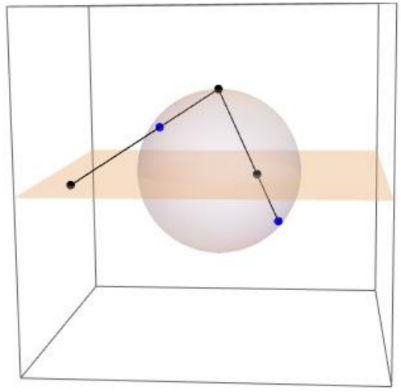
\includegraphics[width=0.5\linewidth]{images/stereographic-projection-map.png}
\caption{The stereographic projection map}
\end{figure}

We remark that the same formula can be written in the alternative form
\[S(z)=\frac{1}{1+|z|^2}\brac{2\Re(z),2\Im(z),|z|^2-1}.\]
As we have seen, $\CC$ may be identified with $\SSS\setminus\{N\}$ by stereographic projection. The set $\SSS\setminus\{N\}$ has a natural metric, namely the one induced from the Euclidean metric on $\RR^3$. This induces a metric $d$ on $\CC$, the unique metric on $\CC$ such that $\SSS$ is an isometry. To spell it out,
\[d(z,w)\coloneqq\norm{S(z)-S(w)}.\]
Here is a formula for this metric.
\begin{lemma}
For any $z,w\in\CC$ we have
\[d(z,w)=\frac{2|z-w|}{\sqrt{1+|z|^2}\sqrt{1+|w|^2}}.\]
\end{lemma}

\begin{proof}
Since $\norm{S(z)}=\norm{S(w)}=1$ we have $\norm{S(z)-S(w)}^2=2-2\langle S(z),S(w)\rangle$, where $\langle,\rangle$ is the usual Euclidean inner product on $\RR^3$. Using the formulae (and after a little computation),
\[\langle S(z),S(w)\rangle=1-\frac{2|z-w|^2}{(1+|z|^2)(1+|w|^2)}.\]
Therefore
\[\norm{S(z)-S(w)}^2=\frac{4|z-w|^2}{(1+|z|^2)(1+|w|^2)}\]
as required.
\end{proof}

\subsection{Adding in $\infty$}
Now it is time to add in the point at infinity, which we will call $\infty$ (note this is just a symbol).

Now (exercise) as $|z|\to\infty$, $S(z)\to N$. Therefore, once we have identified $\CC$ with $\SSS\setminus\{N\}$, it is natural to identify $\infty$ with $N$, and hence $\CC_\infty=\CC\cup\{\infty\}$ with the whole sphere $\SSS$. We extend the map $S$ to a map $S:\CC_\infty\to\SSS$ by defining $S(\infty)=N$.

Using, once again, the Euclidean metric on $S$, we can extend $d$ to a metric on $\CC_\infty$, the unique metric for which the map $S$ is an isometry.

\begin{lemma}
For any $z\in\CC$ we have
\[d(z,\infty)=\frac{2}{\sqrt{1+|z|^2}}.\]
\end{lemma}

\begin{proof}
By definition, $d(z,\infty)=\norm{S(z)-S(\infty)}=\norm{S(z)-N}$, where $N$ is the north pole on the sphere. We may now proceed in much the same way as before, except the calculation is easier this time. The details are left as an exercise.
\end{proof}

We turn now to a few examples, which show that adding $\infty$ to $\CC$ in this way leads to a space with nice analytic properties.

\begin{example}[Translations]
Let $a\in\CC$. Define $f:\CC_\infty\to\CC_\infty$ by $f(z)=z+a$ for $z\in\CC$ and $f(\infty)=\infty$. Then $f$ is a continuous bijection.
\end{example}

\begin{proof}
Clearly $f$ is continuous with respect to the usual metric on $\CC$. Therefore, restricted to $\CC$, it is also continuous with respect to $d$, since $d$ is equivalent to the usual metric.

It remains to check continuity at $\infty$. Let $\epsilon>0$. Now if $\delta>0$ and if $d(z,\infty)<\delta$ then $|z|>\sqrt{\frac{4}{\delta^2}-1}$ and so $|f(z)|>\sqrt{\frac{4}{\delta^2}-1}-|a|$. This tends to $\infty$ as $\delta\to0$, so by choosing $\delta$ small enough in terms of $\epsilon$ it will follows that
\[d\brac{f(z),\infty}=\frac{2}{\sqrt{1+|f(z)|^2}}<\epsilon.\]
\end{proof}

\begin{example}[Dilations]
Let $b\in\CC$. Define $f:\CC_\infty\to\CC_\infty$ by $f(z)=bz$ for $z\in\CC$ and $f(\infty)=\infty$. Then $f$ is a continuous bijection.
\end{example}

\begin{proof}
This is very similar to the argument for translations and we leave the details as an exercise.
\end{proof}

The final example is the most interesting one.

\begin{example}[Inversion]
Define $f:\CC_\infty\to\CC_\infty$ by $f(z)=\frac{1}{z}$ for $z\in\CC\setminus\{0\}$, $f(0)=\infty$ and $f(\infty)=0$. Then $f$ is a continuous bijection.
\end{example}

\begin{proof}
As before, the equivalence of $d$ and the usual metric on $\CC$ means that $f$ is continuous except possibly at $0$ and $\infty$.

We prove that $f$ is continuous at $0$, leaving the continuity at $\infty$ as an exercise (similar to the example on translations).

Let $\epsilon>0$ be small. Then there is $\delta$ such that $\frac{2t}{\sqrt{1+t^2}}\le\epsilon$ for all $t\in[0,\delta]$. If $|z|<\delta$ then
\[d\brac{f(z),f(0)}=d\brac{\frac{1}{z},\infty}=\frac{2}{\sqrt{1+\frac{1}{|z|^2}}}=\frac{2|z|}{\sqrt{1+|z|^2}}\le\epsilon.\]
This indeed shows that $f$ is continuous at $0$.
\end{proof}

\subsection{M\"{o}bius maps}
In this subsection and subsequent ones we look at an important class of maps from $\CC_\infty$ to itself, the M\"{o}bius maps.

\subsection{The complex projective line $\PP^1(\CC)$}
\subsection{Decomposing M\"{o}bius maps}
\subsection{Basic geometry of M\"{o}bius maps}
    \chapter{Complex Functions}\label{chap:complex-functions}
\section{Complex Differentiability}
\begin{definition} \
Suppose $a\in\CC$, $U\subseteq\CC$.
\begin{enumerate}[label=(\roman*)]
\item The \vocab{open ball} of radius $r>0$ centred at $a$ is defined as
\[B_r(a)\coloneqq\{z\in\CC\mid |z-a|<r\}.\]
For the \vocab{closed ball}, we use the condition $|z-a|\le r$ instead.
\item $U$ is \vocab{open} if for every $z\in U$ there exists an open ball $B_r(z)\subset U$.
\item $a$ is a \vocab{boundary point} of $U$ if every $B_r(a)$ contains both points of $U$ and points not in $U$.
%\item $a$ is \vocab{adherent} to $U$ if every $B_r(a)$ contains some element of $U$.
\item $a$ is an \vocab{interior point} of $U$ if there exists $B_r(a)\subset U$.
\item $U$ is \vocab{closed} if it contains all its boundary points. The complement of a closed set is then open.
\item The closure of $U$ is defined to be the union of $U$ and all its boundary points.
\item $U$ is \vocab{bounded} if there exists $C>0$ such that $|z|\le C$ for all $z\in U$.
\end{enumerate}
\end{definition}

\begin{definition}[Limit]
For $f:U\setminus\{a\}\to\CC$, we say that $\displaystyle\lim_{z\to a}f(z)=w$ if $\forall\epsilon>0$, $\exists\delta>0$ such that $\forall z\in U$,
\[0<|z-a|<\delta\implies |f(z)-w|<\epsilon.\]
\end{definition}

\begin{definition}[Continuity]
Let $a\in U$. We say that $f$ is \vocab{continuous} at $a$ if
\[\lim_{z\to a}f(z)=f(a).\]
\end{definition}

\begin{definition}[Convergence]
Given a sequence of complex numbers $(z_n)_{n\in\NN}$, we say that $\displaystyle w=\lim_{n\to\infty}z_n$ if $\forall\epsilon>0$, $\exists N\in\NN\suchthat\forall n\ge N$, $|z_n-w|<\epsilon$.
\end{definition}

\begin{definition}[Cauchy sequence]
$(z_n)$ is a \vocab{Cauchy sequence} if $\forall\epsilon>0$, $\exists N\in\NN\suchthat\forall m,n\ge N$, $|z_n-z_m|<\epsilon$.
\end{definition}

%pg21 of Serge Lang

\begin{definition}[Complex differentiability]
Let $a\in\CC$, and suppose that $f:U\to\CC$ is a function, where $U$ is a neighbourhood of $a$. In particular, $f$ is defined on some ball $B_r(a)$. Then we say that $f$ is (complex) differentiable at $a$ if
\[\lim_{z\to a}\frac{f(z)-f(a)}{z-a}\]
exists. If the limit exists, we write $f^\prime(a)$ for it and call this the derivative of $f$ at $a$.
\end{definition}

Since we will be talking exclusively about functions on $\CC$, we just use the terms differentiable/derivative and omit the word ``complex''. The following lemma collects the basic facts about derivatives. We omit the proof, which is essentially identical to the real case.

\begin{lemma}
Let $a\in\CC$, let $U$ be a neighbourhood of $a$ and let $f,g:U\to\CC$.
\begin{enumerate}[label=(\arabic*)]
\item (Sums, products) If $f,g$ are differentiable at $a$, then $f+g$ and $fg$ are differeitnable at $a$, and
\[(f+g)^\prime(a)=f^\prime(a)+g^\prime(a)\]
and
\[(fg)^\prime(a)=f^\prime(a)g(a)+f(a)g^\prime(a).\]
\item (Quotients) If $f,g$ are differentiable at $a$ and $g(a)\neq0$ then $f/g$ is differentiable at $a$ and
\[\brac{\frac{f}{g}}^\prime(a)=\frac{f^\prime(a)g(a)-f(a)g^\prime(a)}{g(a)^2}.\]
\item (Chain rule) If $U$ and $V$ are open subsets of $\CC$ and $f:V\to U$, $g:U\to\CC$, where $f$ is differentiable at $a\in V$ and $g$ is differeitnable at $f(a)\in U$, then $g\circ f$ is differentiable at $a$, with
\[(g\circ f)^\prime(a)=g^\prime(f(a))f^\prime(a).\]
\end{enumerate}
\end{lemma}

\begin{example}
$f(z)=1$ and $f(z)=z$ are analytic functions from $\CC$ to $\CC$, with derivatives $f^\prime(z)=0$ and $f^\prime(z)=1$ respectively.

Therefore, all polynomials $f(z)=a_nz^n+\cdots+a_1z+a_0$ are analytic, with $f^\prime(z)=na_nz^{n-1}+\cdots+a_1$.
\end{example}

Just as in the real-variable case one can formulate complex differentiability in the following form, which is in fact the better form to use in most instances.

\begin{lemma}
Let $a\in\CC$, let $U$ be a neighbourhood of $a$ and let $f:U\to\CC$. Then $f$ is differentiable at $a$, with derivative $f^\prime(a)$, if and only if we have
\begin{equation}
f(z)=f(a)+f^\prime(a)(z-a)+\epsilon(z)(z-a)
\end{equation}
where $\epsilon(z)\to0$ as $z\to a$.
\end{lemma}

It is an easy exercise to check that this definition is indeed equivalent to (really just a reformulation of) the previous one.

Finally, we give an important definition.

\begin{definition}[Holomorphic function]
Let $U\subseteq\CC$ be an open set (for example, a domain). Let $f:U\to\CC$ be a function. If $f$ is complex differentiable at every $a\in U$, we say that $f$ is \vocab{holomorphic} on $U$.
\end{definition}

\begin{comment}
\begin{definition}[Continuity]
$f:\Omega\to\CC$ for $\Omega\subset\CC$ open is \vocab{continuous} at $z_0$ if $\displaystyle\lim_{z\to z_0}=f(z_0)$.
\end{definition}

\begin{proposition}
$f$ is continuous if and only if $f$ is continuous at all $a\in\Omega$.
\end{proposition}

\begin{proposition}
If $f,g:\Omega\to\CC$ are continuous, then so are $f+g$, $fg$ and $f/g$ (where the last one is defined over $\Omega\setminus\{x\mid g(x)=0\}$).
\end{proposition}

\begin{proposition}
An analytic function is continuous.
\end{proposition}

\begin{proof}
Suppose $f:\Omega\to\CC$ is analytic with derivative 
\[f^\prime(z)=\lim_{h\to0}\frac{f(z+h)-f(z)}{h}.\]
Then
\[\lim_{h\to0}\brac{f(z+h)-f(z)}=f^\prime(z)\lim_{h\to0}h=0.\]
\end{proof}
\end{comment}

\subsection{Cauchy--Riemann Equations}
A function from $\CC$ to $\CC$ may also be thought of as a function from $\RR^2$ to $\RR^2$, and it is useful to study what differentiability means in this language.

Let $a\in\CC$, and let $U$ be a neighbourhood of $a$. Let $f:U\to\CC$ be a function. We abuse notation and identify $\CC\cong\RR^2$ in the usual way, and identify $a$ with $(a_1,a_2)$ (thus $a=a_1+ia_2$). Then (again with some abuse of notation) we may think of $U$ as an open subset of $\RR^2$ and write $f=(u,v)$, where $u,v:\RR^2\to\RR$ (the letters $u,v$ are quite traditional in this context, and sometimes we call these the components of $f$). Another way to think of this is that $f(x+iy)=u(x,y)+iv(x,y)$.

\begin{example}
Consider the function $f(z)=z^2$ (which is holomorphic on all of $\CC$). Since $(x+iy)^2=(x^2-y^2)+2ixy$, we see that the components of $f$ are given by $u(x,y)=x^2-y^2$, $v(x,y)=2xy$.
\end{example}

We have the partial derivatives
\[\pdv{u(a)}{x}\coloneqq\lim_{h\to0}\frac{u(a_1+h,a_2)-u(a_1,a_2)}{h}\]
(if the limit exists) and
\[\pdv{u(a)}{y}\coloneqq\lim_{k\to0}\frac{u(a_1,a_2+k)-u(a_1,a_2)}{k},\]
and similarly for $v$. It is important to note that $h, k$ in these limits are real.

An important fact is that if $f$ is differentiable then these partial derivatives do exist, and moreover they are subject to a constraint.

\begin{theorem}[Cauchy--Riemann equations]
Let $a\in\CC$, let $U$ be a neighbourhood of $a$, and let $f:U\to\CC$ be a function which is complex differentiable at $a$. Let $u,v:\RR^2\to\RR$ be the components of $f$. Then the four partial derivatives $\displaystyle\pdv{u}{x}, \pdv{u}{y}, \pdv{v}{x}, \pdv{v}{y}$ exist at $a$. Moreover, we have the Cauchy--Riemann equations
\begin{equation}
\pdv{u}{x}=\pdv{v}{y}\quad\text{and}\quad\pdv{v}{x}=-\pdv{u}{y}
\end{equation}
and $\displaystyle f^\prime(a)=\pdv{u(a)}{x}+i\pdv{v(a)}{x}$.
\end{theorem}

\begin{proof}
Write $f(z)=u(z)+iv(z)$, where $u,v:\Omega\to\RR$ are real-valued functions. Suppose $f$ is analytic. We compare two ways of taking the limit $f^\prime(z)$:

First take $h$ to be a real number approaching $0$. Then
\[f^\prime(z)=\pdv{f}{x}=\pdv{u}{x}+i\pdv{v}{x}.\]
Next, take $h$ to be purely imaginary, i.e., let $h=ik$ for some $k\in\RR$. Then
\[f^\prime(z)=\lim_{k\to0}\frac{f(z+ik)-f(z)}{ik}=-i\pdv{f}{y}=-i\pdv{u}{y}+\pdv{v}{y}.\]
Comparing real and imaginary parts, we obtain
\[\pdv{f}{x}=-i\pdv{f}{y},\]
or, equivalently,
\[\pdv{u}{x}=\pdv{v}{y}\quad\text{and}\quad\pdv{v}{x}=-\pdv{u}{y}.\]
\end{proof}

Assuming for the time being that $u,v$ have continuous partial derivatives of all orders (and in particular the mixed partials are equal), we can show that
\[\Delta u=\pdv[2]{u}{x}+\pdv[2]{u}{y}=0,\quad\Delta v=\pdv[2]{v}{x}+\pdv[2]{v}{y}=0.\]
Such an equation $\Delta u=0$ is called Laplace's equation and its solution is said to be a harmonic function.

Let us pause to give a simple example using the Cauchy-Riemann equations, which shows that complex differentiation is a much more rigid property than one might think at first sight.

\begin{example}
The function $f(z)=\bar{z}$ is not (complex) differentiable anywhere.
\end{example}

\begin{proof}
Let $u,v:\RR^2\to\RR$ be the components of $f$. Then clearly $u(x,y) = x$, $v(x,y)=-y$ and so $\partial_x u=1,\partial_y u=0, \partial_x v=0, \partial_y v=-1$. Thus $\partial_xu$ is never equal to $\partial_yv$, so the Cauchy--Riemann equations are never satisfied.
\end{proof}

\begin{comment}
$\CC$ is $\RR^2$ with a multiplication. Note that each map $f:\CC\to\CC$ induces a map $f_R:\RR^2\to\RR^2$ (and vice versa).
\begin{example}
Consider $f:\CC\to\CC$, $z\mapsto z^2$.

This is equivalent to $x+iy\mapsto (x+iy)^2=(x^2-y^2)+(2xy)i$.

Thus the mapping is the same as $f_R:\RR^2\to\RR^2$, $(x,y)\mapsto(x^2-y^2,2xy)$.
\end{example}
We want to form a connection between differentiability in $\CC$ and $\RR^2$.
\begin{definition}
A map $f_R:\RR^2\to\RR^2$ is called (totally) differentiable at $\begin{pmatrix}x_0\\ y_0\end{pmatrix}$ if there is a matrix $J\in\RR^{2\times2}$ and a map $\phi:\RR^2\to\RR^2$
\[f_R\brac{\begin{pmatrix}x\\y\end{pmatrix}}=\underbrace{f_R\brac{\begin{pmatrix}x_0\\y_0\end{pmatrix}}+J\brac{\begin{pmatrix}x\\y\end{pmatrix}-\begin{pmatrix}x_0\\ y_0\end{pmatrix}}}_{\text{linear approximation}}+\underbrace{\phi\brac{\begin{pmatrix}x\\ y\end{pmatrix}}}_{\text{error term}}\]
where $\frac{\phi\brac{\begin{pmatrix}x\\ y\end{pmatrix}}}{\norm{\begin{pmatrix}x\\y\end{pmatrix}-\begin{pmatrix}x_0\\ y_0\end{pmatrix}}}\to0$ as $\begin{pmatrix}x\\y\end{pmatrix}\to\begin{pmatrix}x_0\\ y_0\end{pmatrix}$.

$J$ is called the \textbf{Jacobian matrix} of $f_R$ at $\begin{pmatrix}x_0\\y_0\end{pmatrix}\in\RR^2$:
\[J=\begin{pmatrix}
\vdots&\vdots\\
\frac{\partial f_R}{\partial x}&\frac{\partial f_R}{\partial y}\\
\vdots&\vdots
\end{pmatrix}\]
\end{definition}
\begin{example}
Considering the above example, 
\[J=\begin{pmatrix}
2x&-2y\\
2y&2x
\end{pmatrix}.\]
\end{example}
\end{comment}
\else

\fi

%%%%%%%%%%%%%%% TOPOLOGY
\iftop
    \part{Topology}\label{part:topology}
    \chapter{Topological Spaces and Continuous Functions}
\section{Topological Spaces}
\begin{definition}[Topological space]
A \vocab{topological space} $(X,\mathcal{T})$ consists of a non-mepty set $X$ together with a family $\mathcal{T}$ of subsets of $X$ satisfying:
\begin{enumerate}[label=(\arabic*)]
\item $X,\emptyset\in\mathcal{T}$;
\item if $U,V\in\mathcal{T}$, then $U\cap V\in\mathcal{T}$;
\item If $U_i\in\mathcal{T}$ for all $i\in I$, then $\bigcup_{i\in I}U_i\in\mathcal{T}$.
\end{enumerate}
The family $\mathcal{T}$ is called a \vocab{topology} for $X$. The sets in $\mathcal{T}$ are called the \vocab{open sets} of $X$. When $\mathcal{T}$ is understood we talk about the topological space $X$.
\end{definition}

\begin{remark}
A consequence of (2) is that if $U_1,\dots,U_n$ is a collection of open sets, then $U_1\cap\cdots\cap U_n$ is open. But the intersection of infinitely many open sets need not be open!

On the other hand, in (3), the indexing set $I$ is allowed to be infinite. It may even be uncountable.
\end{remark}

\begin{proposition}\label{prop:topo-metrisable}
Let $(X,d)$ be a metric space. Then the open subsets of $X$ form a topology, denoted by $\mathcal{T}_d$.
\end{proposition}

\begin{proof}
Check through the conditions in the definition for a topological space:
\begin{enumerate}[label=(\arabic*)]
\item Trivial.
\item Let $U$ and $V$ be open subsets of $X$. Consider an arbitrary point $x\in U\cap V$.

As $U$ is open, there exists $r_1>0$ such that $B_{r_1}(x)\subseteq U$. Likewise, as $x\in V$ and $V$ is open, there exists $r_2>0$ such that $B_{r_2}(x)\subseteq V$.

Take $r\coloneqq\min\{r_1,r_2\}$. Then $B_r(x)\subseteq B_{r_1}(x)\subseteq U$ and $B_r(x)\subseteq B_{r_2}(x)\subseteq V$. Hence $B_r(x)\subseteq U\cap V$.

\item For every $x\in\bigcup_{i\in I}U_i$ there exists $k\in I$ such that $x\in U_k$. Since $U_k$ is open, there exists $r>0$ such that $B_r(x)\subseteq U_k\subseteq\bigcup_{i\in I}U_i$.
\end{enumerate}
\end{proof}

\begin{example}
The following are some other examples of topological spaces.
\begin{itemize}
\item (Discrete spaces) Let $X$ be any non-empty set. The \textbf{discrete topology} on $X$ is
the set of all subsets of $X$.
\item (Indiscrete spaces) Let $X$ be any non-empty set. The \textbf{indiscrete topology} on $X$ is the family of subsets $\{X,\emptyset\}$.
\item Let $X$ be any non-empty set. The \textbf{co-finite topology} on $X$ consists of the empty set together with every subset $U$ of $X$ such that $X\setminus U$ is finite.
\end{itemize}
\end{example}

\begin{definition}
A topological space $(X,\mathcal{T})$ is \vocab{metrisable} if it arises from (at least oe) metric space $(X,d)$, i.e. there is at least one metric $d$ on $X$ such that $\mathcal{T}=\mathcal{T}_d$.
\end{definition}

\begin{definition}
Two metrics on a set are \vocab{topologically equivalent} if they give rise to the same topology.
\end{definition}

\begin{example} \
\begin{itemize}
\item The metrics $d_1$, $d_2$, $d_\infty$ on $\RR^n$ are all topologically equivalent. (Recall that $d_1$, $d_2$, $d_\infty$ are the metrics arising from the norms $\norm{\cdot}_1$, $\norm{\cdot}_2$, $\norm{\cdot}_\infty$, respectively.)
We shall call the topology defined by the above metrics the \textbf{standard} (or canonical) topology on $\RR^n$.
\item The discrete topology on a non-empty set $X$ is metrisable, using the metric
\[d(x,y)=\begin{cases}
0&\text{if }x=y,\\
1&\text{if }x\neq y.
\end{cases}\]
It is easy to check that this is a metric. To see that is gives the discrete topology, consider any subset $U\subseteq X$. Then for every $x\in U$, $B_\frac{1}{2}(x)\subseteq U$.
\end{itemize}
\end{example}

\begin{definition}
Given two topologies $\mathcal{T}_1$ and $\mathcal{T}_2$ on the same set, we say $\mathcal{T}_1$ is \vocab{coarser} than $\mathcal{T}_2$ if $\mathcal{T}_1\subseteq\mathcal{T}2$.
\end{definition}

\begin{remark}
For any space $(X,\mathcal{T})$, the indiscrete topology on $X$ is coarser than $\mathcal{T}$ which in turn is coarser than the discrete topology on $X$.
\end{remark}

\begin{definition}
Let $(X,\mathcal{T})$ be a topological space. A subset $V$ of $X$ is \vocab{closed} in $X$ if $X\setminus V$ is open in X (i.e. $X\setminus V\in\mathcal{T}$).
\end{definition}

\begin{example} \
\begin{itemize}
\item In the space $[0,1)$ with the usual topology coming from the Euclidean metric, $[1/2,1)$ is closed.
\item In a discrete space, all subsets are closed since their complements are open.
\item In the co-finite topology on a set $X$, a subset is closed if and only if it is finite or all of $X$.
\end{itemize}
\end{example}

\begin{proposition}
Let $X$ be a topological space. Then
\begin{enumerate}[label=(\arabic*)]
\item $X$, $\emptyset$ are closed in $X$;
\item if $V_1$, $V_2$ are closed in $X$ then $V_1\cup V_2$ is closed in $X$;
\item if $V_i$ is closed in $X$ for all $i\in I$ then $\bigcap_{i\in I}Vi$ is closed in $X$.
\end{enumerate}
\end{proposition}

\begin{proof}
These properties follow from (1), (2), (3) of definition of topological space, and from the De Morgan laws.
\end{proof}

\begin{definition}[Convergent sequence]
A sequence $\{x_n\}_{n\in\NN}$ in a topological space $X$ converges to a point $x\in X$ if given any open set $U$ containing $x$ there exists $N\in\NN$ such that $x_n\in U$ for all $n>N$.
\end{definition}

\begin{example} \
\begin{itemize}
\item In a metric space this is equivalent to the metric definition of convergence.
\item In an indiscrete topological space $X$ any sequence converges to any point $x\in X$.
\item In an infinite space $X$ with the co-finite topology any sequence $\{x_n\}$ of pairwise distinct elements (i.e. such that $x_n\neq x_m$ when $n\neq m$) converges to any point $x\in X$.
\end{itemize}
\end{example}



% clear this first https://courses.maths.ox.ac.uk/pluginfile.php/93920/mod_resource/content/1/toplectnotes17%20%281%29.pdf

%https://www.uio.no/studier/emner/matnat/math/MAT4500/h19/rognes-notes-2018.pdf
\else

\fi

%%%%%%%%%%%%%%% MISC
\ifmisc
    \part{Miscellaneous Topics}
    \chapter{Graph Theory}
% ASO: https://courses.maths.ox.ac.uk/pluginfile.php/93815/mod_resource/content/3/GraphTheoryPartA-notes-2023.pdf
% Part B: https://courses.maths.ox.ac.uk/pluginfile.php/25887/mod_resource/content/3/Graph%20Theory%20Lecture%20Notes.pdf

A very early theorem of Graph Theory, perhaps even the first, was proved in 1766 by Euler, concerning a popular problem of the time called ``the bridges of K\"{o}nigsberg''. K\"{o}nigsberg is divided into 4 districts by the river Pregel and has 7 bridges. The problem was to decide whether it is possible to take a walk that crosses every bridge exactly once. To formulate this problem mathematically, we construct a graph in which there is a vertex for each district and an edge representing each bridge.

\section{Introduction to Graphs}
\begin{notation}
$[n]$ denotes the set $\{1,2,\dots,n\}$.
\end{notation}

\begin{notation}
For any set $S$, $\binom{n}{k}$ denotes the set of subsets of $S$ of size $k$; that is,
\[\binom{n}{k}=\{A\subseteq S\mid|A|=k\}.\]
\end{notation}

\begin{definition}[Graph]
A \vocab{graph} is a pair $G=(V(G),E(G))$. The elements of $V(G)$ are called the \vocab{vertices} of $G$; the elements of $E(G)$ are called the \vocab{edges} of $G$.
\end{definition}

$G$ can be represented visually by drawing a point for each vertex and a line between any pair of points that form an edge.

\begin{notation}
$|G|=|V(G)|$ denotes the number of vertices; $e(G)=|E(G)|$ denotes the number of edges.
\end{notation}

\begin{definition}
The \vocab{order} of a graph $G$ is $|V(G)|$. The \vocab{size} of $G$ is $|E(G)|$.
\end{definition}

\begin{definition}
The \vocab{complement} of $G$, denoted by $\overline{G}$, is a graph with the same vertex set as $G$ and $E(\overline{G}) = \{e \notin E(G)\}$; that is, $\overline{G}$ has edges exactly where there are no edges in $G$.
\end{definition}

\begin{notation}
We write $uv=\{u,v\}=vu$ for the (unordered) pair representing an edge between $u$ and $v$.
\end{notation}

\begin{definition}[Simple graph]
A \vocab{loop} is an edge $vv$ for some $v \in V$. An edge $uv$ is a \vocab{multiple edge} if it appears more than once in $E$. 

A graph is \vocab{simple} if it has no loops or multiple edges.
\end{definition}

\begin{remark}
Unless explicitly stated otherwise, we will only consider simple graphs. General (potentially non-simple) graphs are also called multigraphs.
\end{remark}

\begin{definition}
Vertices $u$ and $v$ are \vocab{neighbours} if $uv\in E(G)$; we also say that $u$ and $v$ are \emph{adjacent}. An edge $e\in E(G)$ is \vocab{incident} to a vertex $v \in V(G)$ if $v\in e$. Edges $e$ and $e^\prime$ are \vocab{incident} if $e\cap e^\prime=\emptyset$.
\end{definition}

\begin{definition}
Given a vertex $v$, the \vocab{degree} of $v$, denoted by $d(v)$, is the number of neighbours of $v$ in $G$. If the degree of each vertex is the same, we can call that the degree of the graph.

A \vocab{leaf} is a vertex of degree one, i.e.\ with a unique neighbour.
\end{definition}

\begin{remark}
A trivial graph is a graph with order $1$. An empty graph is a graph of size $0$. Note that a graph must have at least one vertex by definition. But a graph can certainly have no edges!
\end{remark}

\begin{definition}[Subgraph]
$H$ is a \vocab{subgraph} of $G$ if $V(H) \subseteq V(G)$ and $E(H) \subseteq E(G)$.
\begin{itemize}
\item $H$ is a \vocab{spanning subgraph} if $V(H)=V(G)$.
\item $H$ is an \vocab{induced subgraph} if $uv\in E(H)\iff uv\in E(G)$ for all $u,v\in V(H)$.
\end{itemize}
\end{definition}

\begin{definition}[Walk]
A \vocab{$u-v$ walk} in $G$, denoted by $W$, is a finite sequence of vertices 
\[u=v_0,v_1,\dots,v_k=v\]
such that $v_i v_{i+1} \in E(G)$ for all $0 \le i < k-1$.
\begin{itemize}
\item If the vertices in $W$ are distinct, we call it a \vocab{path}.
\item If $u=v$, we call $W$ a \vocab{closed walk}; otherwise, it is an \vocab{open walk}.
\item A \vocab{trail} is an open walk without repeating vertices.
\item A \vocab{path} is an open walk without repeating edges. Note that paths are trails, but not vice-versa.
\item A \vocab{circuit} is a closed walk without repeating edges, i.e. $u=v$, it begins and ends with the same vertex.
\item A \vocab{cycle} is a closed walk without repeating vertices, other than the initial and terminal vertices, i.e. $u=v$ but the vertices are otherwise distinct and $W$ has at least 3 vertices. If a graph $G$ has no cycle we call it \vocab{acyclic}.
\item A \vocab{trail} is a walk in which no two vertices appear consecutively (in either order) more than once; that is, no edge is used more than once. A \vocab{tour} is a closed trail.
\end{itemize}
\end{definition}

\begin{definition}[Connectedness]
A graph $G$ is \vocab{connected} if there exists a $u-v$ path for all $u,v\in V(G)$.

Vertices $u,v\in V(G)$ \vocab{lie in the same component} if they are joined by a $u-v$ walk. Clearly this forms an equivalence relation and the partition of $V(G)$ into equivalence classes expresses $G$ as a union of disjoint connected graphs called its \vocab{components}.
\end{definition}

\begin{definition}[Diameter]
The \vocab{diameter} of a connected graph $G$, denoted by $\diam G$, is defined as
\[\diam G=\max_{u\neq v}d(u,v).\]
By construction, $d(u,v) \le \diam G$ for all $u,v \in V(G)$.
\end{definition}

\begin{definition}[Complete graph]
$G$ is \vocab{complete} if every pair of vertices in $G$ is joined by an edge. A complete graph on $n$ vertices is denoted by $K_n$.
\end{definition}

\begin{definition}
A graph $G$ is \vocab{planar} if it can be drawn such that a pair of edges can only cross at a vertex.
\end{definition}

\begin{theorem}[Euler's Characteristic Formula]
For any connected planar graph, with $V$ vertices, $E$ edges and $F$ faces (regions bounded by edges, including the outer, infinitely large region), then
\begin{equation}
V-E+F=2.
\end{equation}
\end{theorem}

\begin{proof}
We prove by induction.

If $G$ has zero edges, that is $E=0$, then $V=1$ and $F=1$. Then $V-E+F=1-0+1=2$.

Suppose Euler's formula holds for a graph with $n$ edges.

For a graph $G$ with $n+1$ edges, we now consider two cases:

\textbf{Case 1}: If $G$ is a tree and does not contain any cycle. It can be easily proven by induction for trees with any number of edges.

\textbf{Case 2}: If $G$ is not a tree and contains at least one cycle. Choose an edge $e_1$ in $G$ which divides the given region into two different parts and remove that edge $e_1$ to get another graph $G^\prime$. Note that $F>F^\prime$.

Now, $G$ has $n+1$ edges, then $G^\prime$ has $n$ edges so by the hypothesis $G^\prime$ satisfies the Euler's formula. For $G^\prime$, $V^\prime-E^\prime+F^\prime=2$ where $V^\prime=V$, $E^\prime=E-1$ and $F^\prime=F-1$.

Substituting these values gives
\begin{align*}
V^\prime-E^\prime+F^\prime&=2\\
V-E+1+F-1&=2\\
V-E+F&=2
\end{align*}

Hence, Euler's formula is applicable for $n+1$ edges.

This proves the Euler's formula.
\end{proof}

\subsection{Trees}
\begin{definition}[Tree]
A \vocab{tree} is a connected graph that does not contain any cycles; that is, it is a minimally connected graph.
\end{definition}

\begin{proposition}\label{prop:tree-acyclic}
Any tree is acyclic.
\end{proposition}

\begin{proof}
Let $G$ be a tree, i.e. $G$ is minimally connected.

Suppose, for a contradiction, that $G$ contains a cycle $C$. Let $e \in E(C)$. We will obtain our contradiction by showing that $G-e \coloneqq (V(G),E(G)\setminus\{e\})$ is connected. 

Let $P$ be the path obtained by deleting $e$ from $C$. Consider any $u,v$ in $V(G)$. As $G$ is connected, there is an $u-v$ walk $W$ in $G$. Replacing any use of $e$ in $W$ by $P$ gives an $u-v$ walk in $G-e$. Thus $G-e$ is connected, a contradiction.
\end{proof}

The following are equivalent characterisations of trees.
\begin{lemma}[Characterisation of trees]\label{lemma:tree-char} \
\begin{enumerate}[label=(\roman*)]
\item $G$ is a tree if and only if $G$ is connected and acyclic.
\item Any two vertices in a tree are joined by a unique path.
\end{enumerate}
\end{lemma}

\begin{proof} \
\begin{enumerate}[label=(\roman*)]
\item If $G$ is a tree then $G$ is connected and acyclic.

Conversely, let $G$ be connected and acyclic. Suppose for a contradiction that $G-e$ is connected for some $e = (u,v) \in E(G)$.

Let $W$ be a shortest $u-v$ walk in $G-e$. Then $W$ must be a path, i.e. have no repeated vertices, otherwise we would find a shorter walk by deleting a segment of $W$ between two visits to the same vertex. Combining $W$ with $(u,v)$ gives a cycle, which is a contradiction.

\item Suppose for a contradiction that this fails for some tree $G$. 

Choose $u,v$ in $V(G)$ so that there are distinct $u-v$ paths P1, P2, and P1 is as short as possible over all such choices of $u$ and $v$.

Then P1 and P2 only intersect in $u$ and $v$, so their union is a cycle, contradicting \cref{prop:tree-acyclic}.
\end{enumerate}
\end{proof}

\begin{remark}
The fact that a shortest walk between two points is a path is often useful. More generally, considering an extremal (shortest, longest, minimal, maximal, \dots) object is often a useful proof technique.
\end{remark}

\begin{lemma}\label{tree_leaves}
Any tree with at least two vertices has at least two leaves.
\end{lemma}
\begin{proof}
Consider any tree $G$. Let $P$ be a longest path in $G$. The two ends of $P$ must be leaves. Indeed, an end cannot have a neighbour in $V(G) \setminus V(P)$, or we could make $P$ longer, and cannot have any neighbour in $V(P)$ other than the next in the sequence of $P$, or we would have a cycle.

The existence of leaves in trees is useful for inductive arguments, via the following lemma. Given $v \in V(G)$, let $G-v$ be the graph with $V(G-v) = V(G)\setminus\{v\}$ and $E(G-v) = \{(u,v) \in E(G) \mid v \notin \{u,v\}\}$.
\end{proof}

\begin{lemma}\label{tree_leaf}
If $G$ is a tree and $v$ is a leaf of $G$ then $G-v$ is a tree.
\end{lemma}
\begin{proof}
By \cref{lemma:tree-char} (i), it suffices to show that $G-v$ is connected and acyclic. Acyclicity is immediate from \cref{prop:tree-acyclic}. Connectedness follows by noting for any $u,v \in V(G)\setminus\{v\}$ that the unique $u-v$ path in $G$ is contained in $G-v$.
\end{proof}

\begin{lemma}\label{tree_edges}
Any tree on $n$ vertices has $n-1$ edges.
\end{lemma}
\begin{proof}
By induction. A tree with 1 vertex has 0 edges. Let $G$ be a tree on $n>1$ vertices. By \cref{tree_leaves}, $G$ has a leaf $v$. By \cref{tree_leaf}, $G-v$ is a tree. By induction hypothesis, $G-v$ has $n-2$ edges. Replacing $v$ gives $n-1$ edges in $G$.
\end{proof}

We conclude this section with another characterisation of trees. First we note that any connected graph $G$ contains a minimally connected subgraph (i.e. a tree) with the same vertex set, which we call a \vocab{spanning tree} of $G$.

\begin{lemma}
A graph $G$ is a tree on $n$ vertices if and only if $G$ is connected and has $n-1$ edges.
\end{lemma}

\begin{proof}
If $G$ is a tree then $G$ is connected by definition and has $n-1$ edges by \cref{tree_edges}. 

Conversely, suppose that $G$ is connected and has $n-1$ edges. Let $H$ be a spanning tree of $G$. Then $H$ has $n-1$ edges by \cref{tree_edges}, so $H = G$, so $G$ is a tree.
\end{proof}

\subsection{Bipartite Graphs, Matching}
\begin{definition}[Bipartite graph]
A graph $G$ is \vocab{bipartite} if $V(G)$ can be partitioned into two non-empty disjoint sets $A$ and $B$ such that no edge has both endpoints in the same set.

$G$ is said to be \vocab{complete bipartite} if $G$ is bipartite and all possible edges between the two sets $A$ and $B$ are drawn. In the case where $|A|=m, |B|=n$, such a graph is denoted by $K_{m,n}$.

Let $k \ge 2$. A graph $G$ is said to be \vocab{$k$-partite} if $V(G)$ can be partitioned into $k$ pairwise disjoint sets $A_1, \dots, A_k$ such that no edge has both endpoints in the same set.

A \vocab{complete $k$-partite} graph is defined similarly as a complete bipartite. In the case where $|A_i| = n_i$, such a graph is denoted by $K_{n_1,n_2,\dots,n_k}$.
\end{definition}

The Marriage Problem is as follows:

\begin{quote}
Given $n$ men and $n$ women, under what conditions is it possible to pair each man with a woman such that every pair know each other?
\end{quote}

We now mathematically formulate this problem. Let $G$ be a graph. We say $M\subseteq E(G)$ is a \emph{matching} if the edges in $M$ are pairwise disjoint. We say $M$ is \emph{perfect} if every vertex belongs to some edge of $M$. 
In this terminology, the marriage problem asks when a bipartite graph has a perfect matching.

We will return to this question later. First we consider the algorithmic question of how to find a matching of maximum size.

\begin{theorem}[K\"{o}nig's Theorem]
In any bipartite graph, the size of a maximum matching equals the size of a minimum cover.
\end{theorem}

\begin{theorem}[Hall's Theorem]
Let $G$ be a bipartite graph with parts $A$ and $B$. Then $G$ has a matching covering $A$ if and only if $|N(S)|\ge|S|$ for every $S\subseteq A$.
\end{theorem}

\subsection{Isomorphism}
\begin{definition}[Isomorphism]
Let $G_1 = (V_1, E_1)$ and $G_2 = (V_2, E_2)$ be graphs. An isomorphism $\phi : G_1 \to G_2$ is a bijection (a one-to-one correspondence) from $V_1$ to $V_2$ such that $(u,v) \in E_1$ if and only if $(\phi(u),\phi(v)) \in E_2$. We say $G_1$ is isomorphic to $G_2$ if there is an isomorphism between them.
\end{definition}

\subsection{Minimum Cost Spanning Trees}
$G$ is a connected graph and we have some cost $c(e)>0$ for every edge $e\in E(G)$. For any $S\subseteq E(G)$ we call $c(S)=\sum_{e\in S}c(e)$ the cost of $S$. The problem we wish to solve is:

\begin{quote}
Find $S\subseteq E(G)$ with minimum possible $c(S)$ such that $(V(G),S)$ is a connected graph.
\end{quote}

A solution is necessarily a spanning tree for $G$. Recall that this is a tree $T=(V(G),S)$ where $S\subseteq E(G)$. We say that $T$ is a minimum cost spanning tree of $G$ if any other spanning tree $T^\prime$ satisfies $c(T^\prime)\ge c(T)$. How can we find one efficiently?

One natural method to try is the ``greedy algorithm'': choose edges one at a time, each time choosing the cheapest edge that does not create a cycle. There are various versions of this algorithm; we will describe the one due to Kruskal.

\begin{theorem}[Kruskal's Algorithm]
At step $i\ge0$, keep track of a subset $A_i\subseteq E(G)$. This will have the property that $(V(G),A_i)$ is acyclic. Start with $A_0=\emptyset$. At step $i\ge0$, is there an edge $e\in E(G)\setminus A_i$ such that $(V(G),A_i\cup\{e\})$ is acyclic? If no, then output $A=A_i$ and stop. If yes, then set $A_{i+1}=A_i\cup\{e\}$ for one such $e$ such that $c(e)$ is minimal, and proceed to step $i+1$.
\end{theorem}

You should try a few examples on small graphs to understand the algorithm and check that it does find minimum cost spanning trees in your examples. However, it is not obvious that it will always work, and indeed there are different problems in graph theory for which greedy algorithms don't always work. Fortunately, the greedy algorithm always works for the minimum cost spanning tree problem, as shown by the following theorem.

\begin{theorem}
$(V(G),A)$ is a minimum cost spanning tree of $G$.
\end{theorem}

\begin{proof}

\end{proof}

\subsection{Euler Tours and Trails}
\begin{definition}
Let $W$ be a walk in a graph $G$. We call $W$ an \vocab{Euler trail} if every edge of $G$ appears exactly once in $W$. 

We call $W$ an \vocab{Euler tour} if it is closed, i.e. it starts and ends at the same vertex.
\end{definition}

For a graph $G$ with an Euler tour $W$, clearly $G$ must be connected after we delete all isolated vertices (i.e. vertices of degree zero). We also note that each visit of $W$ to a vertex v uses two edges at v (one to arrive and one to leave). This is also true of the start and end vertex of W if we consider them to be a single visit. (Or we can think of the vertex sequence of W as being written around a circle rather than along a line, so that there is no start or end, and each visit uses two edges.) As every edge is used exactly once, we deduce that every vertex has even degree; we call a graph with this property \vocab{Eulerian}.

\begin{lemma}
In any graph, there are an even number of vertices with odd degree.
\end{lemma}

\begin{proof}
Since every edge has two endpoints,
\[\sum_{v\in V(G)}d(v)=2|E(G)|.\]
Therefore, in the sum, there must be an even number of occurrences of $d(v)$ for which $d(v)$ is odd.
\end{proof}

An Euler tour can be found efficiently using \vocab{Fleury's Algorithm}:
\begin{quote}
Start at any vertex. We will follow a walk, erasing each edge after it is used (erased edges cannot be used again). At each stage, ensure that the following holds:
\begin{enumerate}[label=(\roman*)]
\item when the edge is removed, the resulting graph is connected once isolated vertices are removed, and
\item we do not run along an edge to a leaf, unless this is the only edge of the graph.
\end{enumerate}
\end{quote}

\begin{theorem}[Euler]
Let $G$ be a connected Eulerian graph. Then $G$ has an Euler tour.
\end{theorem}

\subsection{Hamiltonian Cycles}
In the previous section, we investigated graphs that admit an Euler tour, which is a closed walk that traverses every edge exactly once. There is a seemingly related question that one can ask about a graph: does there exists a closed walk that visits every vertex exactly once?

\begin{definition}[Hamiltonian cycle]
A \vocab{Hamiltonian cycle} is a closed walk that visits every vertex of a graph $G$ once.

When a graph $G$ contains such a cycle, it is said to be \vocab{Hamiltonian}.
\end{definition}

\begin{theorem}[Ore's Theorem]
Let $G$ be a connected graph with $n\ge3$ vertices. Suppose that for every pair of non-adjacent vertices $x$ and $y$, $d(x)+d(y)\ge n$. Then $G$ is Hamiltonian.
\end{theorem}

\begin{proof}

\end{proof}

\begin{corollary}[Dirac's Theorem]
If $G$ is connected with $n\ge3$ vertices and for every vertex $v$, $d(v)\ge\frac{n}{2}$, then $G$ is Hamiltonian.
\end{corollary}

\subsection{Shortest Paths}
How do you find the quickest route from A to B? Maybe you ask your satnav, but how does your satnav find the route? It doesn't check all options, as there are too many: it uses an efficient algorithm. We formulate the problem mathematically as follows:

\begin{quote}
Let $G$ be a connected graph. Let $\ell(e)>0$ be the ``length'' of the edge $e$ for $e\in E(G)$. The $\ell$-length of a path $P$ is $\ell(P)=\sum_{e\in E(P)}\ell(e)$.

Given $x,y\in V(G)$, an $\ell$-shortest $xy$-path is an $xy$-path $P$ that minimises $\ell(P)$.
\end{quote}

The \vocab{Dijkstra's Algorithm} is a method of finding a $\ell$-shortest $xy$-path. The idea of the algorithm is to maintain a ``tentative distance from $x$'' called $D(v)$ for each $v\in V(G)$. At each step of the algorithm we finalise $D(u)$ for some vertex $u$. At the end of the algorithm all $D(u)$ will be equal to the correct value, i.e. $D(u)=\ell(P_u^*)$ for some $\ell$-shortest $xu$-path $P_u^*$.

\subsection{Chinese Postman Problem}

\subsection{Colouring}
vertex/edge colouring and Ramsey Theory
graph colouring and the four-colour theorem; Ramsey theory; 

\subsection{Tur\'{a}n graph}


Menger's theorem, network flows; complete subgraphs and Turán's theorem, and the Erdös-Stone theorem; probabilistic methods in graph theory
\pagebreak

\section*{Exercises}
Problems can include tournament, matching, and scheduling problems.
\begin{prbm}[K\"{o}nigsberg Bridge Problem]
K\"{o}nigsberg was a small town in Prussia. There is a river running through the town and there were seven bridges across the river. The inhabitants of K\"{o}nigsberg liked to walk around the town and cross all of the bridges:

Is it possible to walk around the town and cross every bridge, once and once only?
\end{prbm}

\begin{solution}
We replace every landmass by a vertex and every bridge by an edge to give the following graph.
\end{solution}

\begin{prbm}(Moser's circle problem) 
Determine the number of regions into which a circle is divided if $n$ points on its circumference are joined by chords with no three internally concurrent.
\end{prbm}

\begin{proof}[Solution]
Consider the graph which has points on the circumference and intersection points between chords as its vertices.

Let $V, E, F$ denote the number of vertices, edges, regions respectively.

To count the number of intersection points, note that $4$ points on the circumference give one unique intersection point between the two non-parallel chords formed by connecting two pairs of points which intersect inside the circle. Hence, number of intersection points is $\dbinom{n}{4}$. 
\[ V = n + \binom{n}{4} \]
Total number of edges includes $n$ circular arcs, number of original chords formed from connecting pairs of points on the circumference
E = no. of original lines + 2 x no. of intersection points
E = n choose 2 + 2 x n choose 4 + n
since there are n circular arcs

Using Euler's Characteristic Formula, we have 
\begin{align*}
F &= E - V - 1 \\
\Aboxed{F &= 1 + \binom{n}{2} + \binom{n}{4}}
\end{align*}
\end{proof}

\begin{comment}
\chapter{Game Theory}
\textbf{Recommended readings:} \href{https://mathematicalolympiads.files.wordpress.com/2012/08/martin_j-_osborne-an_introduction_to_game_theory-oxford_university_press_usa2003.pdf}{``An Introduction to Game Theory" by Osborne}
%http://www.matt-versaggi.com/mit_open_courseware/GameAI/MathematicalGameTheoryandApplications.pdf

% games of normal form and extensive form, and their applications in economics, relations between game theory and decision making; games of complete information: static games with finite or infinite strategy spaces, Nash equilibrium of pure and mixed strategy, dynamic games, backward induction solutions, information sets, subgame-perfect equilibrium, finitely and infinitely-repeated games; games of incomplete information: Bayesian equilibrium, first price sealed auction, second price sealed auction, and other auctions, dynamic Bayesian games, perfect Bayesian equilibrium, signaling games; cooperative games: bargaining theory, cores of n-person cooperative games, the Shapley value and its applications in voting, cost sharing, etc.

\section{Strict Dominance}
\subsection{Prisoner's Dilemma}
To start off, we will take a look at the \vocab{Prisoner's Dilemma}, which goes as follows:

\begin{quote}
Two thieves plan to rob a store, but the police arrest them for trespassing. The police suspect that they planned to break in but lack the evidence to support such an accusation. They require a confession to charge the suspects. The police offer them the following deal:
\begin{itemize}
\item If no one confesses, both are charged a one month jail sentence each for trespassing.
\item If a rat confesses and the other does not, the rat is not charged but the other is charged a twelve month jail sentence for robbery.
\item If both confess, both are charged an eight month jail sentence each.
\end{itemize}
If both criminals are self-interested and only care about minimising their jail time, should they take the interrogator's deal?
\end{quote}

We condense the above information into a \vocab{payoff matrix} as shown below, where we have two players, A and B. The horizontal rows represent A's choices, while the vertical columns represent B's choices, and each cell contains a combination of their payoffs.

\begin{table}[H]
\centering
\begin{tabular}{rcc}
\multicolumn{1}{l}{}         & quiet                       & confess                     \\ \cline{2-3} 
\multicolumn{1}{r|}{quiet}   & \multicolumn{1}{c|}{$-1$, $-1$} & \multicolumn{1}{c|}{$-12$, $0$} \\ \cline{2-3} 
\multicolumn{1}{r|}{confess} & \multicolumn{1}{c|}{$0$, $-12$} & \multicolumn{1}{c|}{$-8$, $-8$} \\ \cline{2-3} 
\end{tabular}
\end{table}

\subsection{Split or Steal}
The game goes as follows:
\begin{quote}
Each of two players, Sarah and Steve, has to pick one of two balls: inside one ball appears the word ``\textbf{split}'' and inside the other the word ``\textbf{steal}'' (each player is first asked to secretly check which of the two balls in front of him/her is the split ball and which is the steal ball). They make their decisions simultaneously. 
\end{quote}

The possible outcomes are shown in the figure below, where each row is labelled with a possible choice for Sarah and each column with a possible choice for Steven. Each cell in the table thus corresponds to a possible pair of choices and the resulting outcome is written inside the cell.

\begin{figure}[H]
    \centering
    \includegraphics[width=12cm]{images/Split_or_steal.png}
\end{figure}

\section{Nash Equilibrium}
\vocab{Nash Equilibrium} is a set of optimal strategies that work against \textit{all} counter-steategies. This means that if any given player were told the strategies of all their opponents, they still would choose to retain their original strategy. 

\subsection{Matrix games}

\section{Fair Division}
\subsection{Rental harmony problem}
Sperner's lemma

%https://www.cs.cmu.edu/~arielpro/15896/docs/paper19b.pdf
\end{comment}
    \chapter{Logic}
Mathematical logic is about providing a uniform, unambiguous language for mathematics, making precise what a proof is, explaining and guaranteeing exactness, rigour and certainty in mathematics, as well as establishing the foundations of mathematics.

\section{Propositional Calculus}
This section is basically a recap of \cref{chap:logic-proofs}.

The alphabet of propositional calculus consists of the following (abstract) symbols:
\begin{itemize}
\item the \vocab{propositional variables} $p_0,p_1,\dots,p_n,\dots$
\item \vocab{negation} $\lnot$ - the unary connective not
\item four binary connectives $\rightarrow,\land,\lor,\leftrightarrow$ which mean implies, and, or, if and only if respectively
\item two punctuation marks $($ and $)$ which are left parenthesis and right parenthesis respectively.
\end{itemize}

This alphabet is denoted by $\mathcal{L}$.

\begin{notation}
Note also that we use $\rightarrow$, and not $\implies$.
\end{notation}

\begin{definition}[String]
A \vocab{string} (from $\mathcal{L}$) is any finite sequence of symbols from $\mathcal{L}$.
\end{definition}

\begin{example} \
\begin{itemize}
\item $\rightarrow p_{17}()$
\item $((p_0\land p_1)\rightarrow\lnot p_2)$
\item $))\lnot)p_{32}$
\end{itemize}
\end{example}

The \vocab{length} of a string is the number of symbols in it. So the strings in the examples have length 4, 10, 5 respectively. (A propositional variable has length 1.)

We now single out from all strings those which make grammatical sense (formulas).

\begin{definition}[Formula]
The notion of a \vocab{formula} of $\mathcal{L}$ is defined (recursively) by the following rules:
\begin{enumerate}[label=(\roman*)]
\item every propositional variable is a formula
\item if the string $A$ is a formula then so is $\lnot A$
\item if the strings $A$ and $B$ are both formulas then so are the strings
\begin{align*}
(A\rightarrow B)&\text{ read $A$ implies $B$}\\
(A\land B)&\text{ read $A$ and $B$}\\
(A\lor B)&\text{ read $A$ or $B$}\\
(A\leftrightarrow B)&\text{ read $A$ if and only if $B$}
\end{align*}
\item Nothing else is a formula, i.e. a string $\phi$ is a formula if and only if $\phi$ can be obtained from propositional variables by finitely many applications of the formation rules (ii) and (iii)
\end{enumerate}
\end{definition}
\else

\fi
\pagebreak

\backmatter
\printbibliography[title={Bibliography}]

\printindex
\end{document}